% Options for packages loaded elsewhere
\PassOptionsToPackage{unicode}{hyperref}
\PassOptionsToPackage{hyphens}{url}
%
\documentclass[
]{book}
\usepackage{amsmath,amssymb}
\usepackage{lmodern}
\usepackage{iftex}
\ifPDFTeX
  \usepackage[T1]{fontenc}
  \usepackage[utf8]{inputenc}
  \usepackage{textcomp} % provide euro and other symbols
\else % if luatex or xetex
  \usepackage{unicode-math}
  \defaultfontfeatures{Scale=MatchLowercase}
  \defaultfontfeatures[\rmfamily]{Ligatures=TeX,Scale=1}
\fi
% Use upquote if available, for straight quotes in verbatim environments
\IfFileExists{upquote.sty}{\usepackage{upquote}}{}
\IfFileExists{microtype.sty}{% use microtype if available
  \usepackage[]{microtype}
  \UseMicrotypeSet[protrusion]{basicmath} % disable protrusion for tt fonts
}{}
\makeatletter
\@ifundefined{KOMAClassName}{% if non-KOMA class
  \IfFileExists{parskip.sty}{%
    \usepackage{parskip}
  }{% else
    \setlength{\parindent}{0pt}
    \setlength{\parskip}{6pt plus 2pt minus 1pt}}
}{% if KOMA class
  \KOMAoptions{parskip=half}}
\makeatother
\usepackage{xcolor}
\usepackage{color}
\usepackage{fancyvrb}
\newcommand{\VerbBar}{|}
\newcommand{\VERB}{\Verb[commandchars=\\\{\}]}
\DefineVerbatimEnvironment{Highlighting}{Verbatim}{commandchars=\\\{\}}
% Add ',fontsize=\small' for more characters per line
\usepackage{framed}
\definecolor{shadecolor}{RGB}{248,248,248}
\newenvironment{Shaded}{\begin{snugshade}}{\end{snugshade}}
\newcommand{\AlertTok}[1]{\textcolor[rgb]{0.94,0.16,0.16}{#1}}
\newcommand{\AnnotationTok}[1]{\textcolor[rgb]{0.56,0.35,0.01}{\textbf{\textit{#1}}}}
\newcommand{\AttributeTok}[1]{\textcolor[rgb]{0.77,0.63,0.00}{#1}}
\newcommand{\BaseNTok}[1]{\textcolor[rgb]{0.00,0.00,0.81}{#1}}
\newcommand{\BuiltInTok}[1]{#1}
\newcommand{\CharTok}[1]{\textcolor[rgb]{0.31,0.60,0.02}{#1}}
\newcommand{\CommentTok}[1]{\textcolor[rgb]{0.56,0.35,0.01}{\textit{#1}}}
\newcommand{\CommentVarTok}[1]{\textcolor[rgb]{0.56,0.35,0.01}{\textbf{\textit{#1}}}}
\newcommand{\ConstantTok}[1]{\textcolor[rgb]{0.00,0.00,0.00}{#1}}
\newcommand{\ControlFlowTok}[1]{\textcolor[rgb]{0.13,0.29,0.53}{\textbf{#1}}}
\newcommand{\DataTypeTok}[1]{\textcolor[rgb]{0.13,0.29,0.53}{#1}}
\newcommand{\DecValTok}[1]{\textcolor[rgb]{0.00,0.00,0.81}{#1}}
\newcommand{\DocumentationTok}[1]{\textcolor[rgb]{0.56,0.35,0.01}{\textbf{\textit{#1}}}}
\newcommand{\ErrorTok}[1]{\textcolor[rgb]{0.64,0.00,0.00}{\textbf{#1}}}
\newcommand{\ExtensionTok}[1]{#1}
\newcommand{\FloatTok}[1]{\textcolor[rgb]{0.00,0.00,0.81}{#1}}
\newcommand{\FunctionTok}[1]{\textcolor[rgb]{0.00,0.00,0.00}{#1}}
\newcommand{\ImportTok}[1]{#1}
\newcommand{\InformationTok}[1]{\textcolor[rgb]{0.56,0.35,0.01}{\textbf{\textit{#1}}}}
\newcommand{\KeywordTok}[1]{\textcolor[rgb]{0.13,0.29,0.53}{\textbf{#1}}}
\newcommand{\NormalTok}[1]{#1}
\newcommand{\OperatorTok}[1]{\textcolor[rgb]{0.81,0.36,0.00}{\textbf{#1}}}
\newcommand{\OtherTok}[1]{\textcolor[rgb]{0.56,0.35,0.01}{#1}}
\newcommand{\PreprocessorTok}[1]{\textcolor[rgb]{0.56,0.35,0.01}{\textit{#1}}}
\newcommand{\RegionMarkerTok}[1]{#1}
\newcommand{\SpecialCharTok}[1]{\textcolor[rgb]{0.00,0.00,0.00}{#1}}
\newcommand{\SpecialStringTok}[1]{\textcolor[rgb]{0.31,0.60,0.02}{#1}}
\newcommand{\StringTok}[1]{\textcolor[rgb]{0.31,0.60,0.02}{#1}}
\newcommand{\VariableTok}[1]{\textcolor[rgb]{0.00,0.00,0.00}{#1}}
\newcommand{\VerbatimStringTok}[1]{\textcolor[rgb]{0.31,0.60,0.02}{#1}}
\newcommand{\WarningTok}[1]{\textcolor[rgb]{0.56,0.35,0.01}{\textbf{\textit{#1}}}}
\usepackage{longtable,booktabs,array}
\usepackage{calc} % for calculating minipage widths
% Correct order of tables after \paragraph or \subparagraph
\usepackage{etoolbox}
\makeatletter
\patchcmd\longtable{\par}{\if@noskipsec\mbox{}\fi\par}{}{}
\makeatother
% Allow footnotes in longtable head/foot
\IfFileExists{footnotehyper.sty}{\usepackage{footnotehyper}}{\usepackage{footnote}}
\makesavenoteenv{longtable}
\usepackage{graphicx}
\makeatletter
\def\maxwidth{\ifdim\Gin@nat@width>\linewidth\linewidth\else\Gin@nat@width\fi}
\def\maxheight{\ifdim\Gin@nat@height>\textheight\textheight\else\Gin@nat@height\fi}
\makeatother
% Scale images if necessary, so that they will not overflow the page
% margins by default, and it is still possible to overwrite the defaults
% using explicit options in \includegraphics[width, height, ...]{}
\setkeys{Gin}{width=\maxwidth,height=\maxheight,keepaspectratio}
% Set default figure placement to htbp
\makeatletter
\def\fps@figure{htbp}
\makeatother
\setlength{\emergencystretch}{3em} % prevent overfull lines
\providecommand{\tightlist}{%
  \setlength{\itemsep}{0pt}\setlength{\parskip}{0pt}}
\setcounter{secnumdepth}{5}
\usepackage{booktabs}
\usepackage{booktabs}
\usepackage{longtable}
\usepackage{array}
\usepackage{multirow}
\usepackage{wrapfig}
\usepackage{float}
\usepackage{colortbl}
\usepackage{pdflscape}
\usepackage{tabu}
\usepackage{threeparttable}
\usepackage{threeparttablex}
\usepackage[normalem]{ulem}
\usepackage{makecell}
\usepackage{xcolor}
\ifLuaTeX
  \usepackage{selnolig}  % disable illegal ligatures
\fi
\usepackage[]{natbib}
\bibliographystyle{plainnat}
\IfFileExists{bookmark.sty}{\usepackage{bookmark}}{\usepackage{hyperref}}
\IfFileExists{xurl.sty}{\usepackage{xurl}}{} % add URL line breaks if available
\urlstyle{same} % disable monospaced font for URLs
\hypersetup{
  pdftitle={Interactions et modifications d'effet   en Epidémiologie},
  pdfauthor={CERPOP, INSERM, EQUITY Team},
  hidelinks,
  pdfcreator={LaTeX via pandoc}}

\title{Interactions et modifications d'effet en Epidémiologie}
\author{CERPOP, INSERM, EQUITY Team}
\date{Last compiled on 09 June, 2023}

\begin{document}
\maketitle

{
\setcounter{tocdepth}{1}
\tableofcontents
}
\hypertarget{pruxe9sentation}{%
\chapter{Présentation}\label{pruxe9sentation}}

Ce document a été rédigé en tant que document de synthèse du travail du groupe ``Interaction'' de l'équipe EQUITY, CERPOP.
Ce travail a consisté en une revue de la littérature et en une application détaillée des méthodes sur des analyses illustratives, dans un but d'auto-formation et pédagogique.

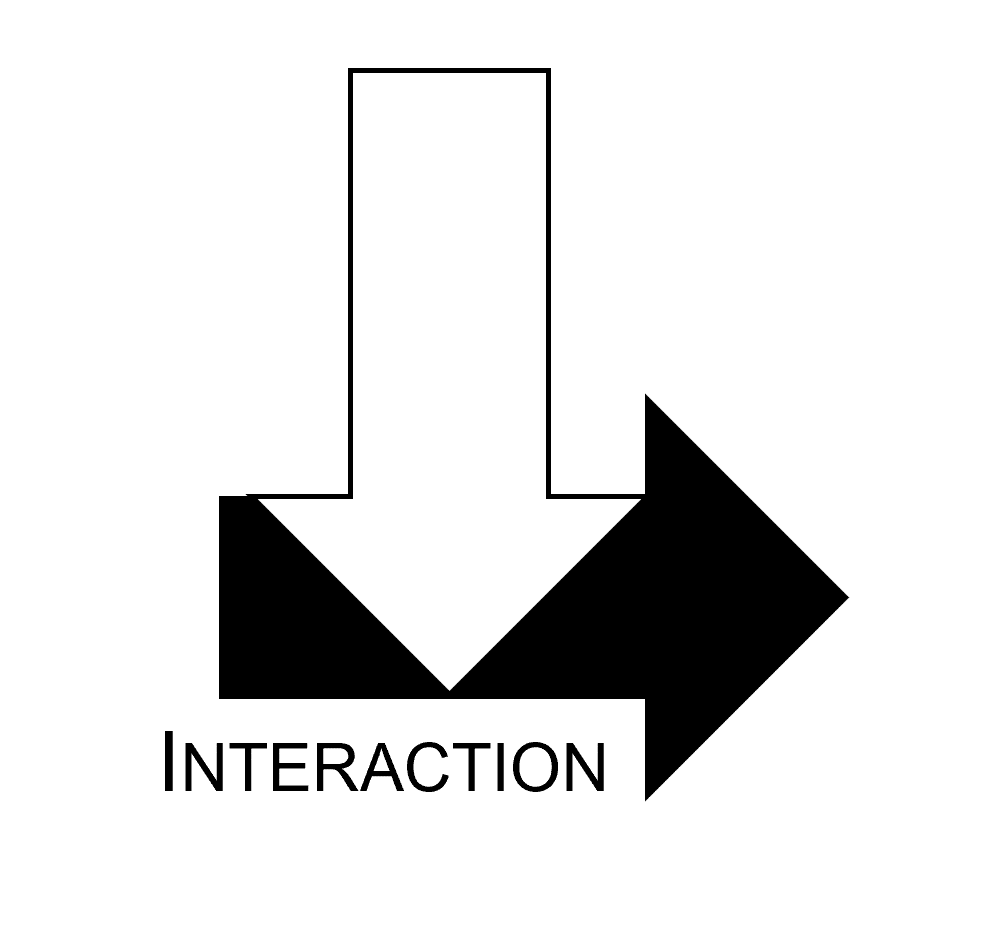
\includegraphics[width=0\textwidth,height=\textheight]{img/Image0.png}

Les participant.e.s du groupe de travail sont :

\begin{itemize}
\tightlist
\item
  Hélène COLINEAUX\\
\item
  Léna BONIN
\item
  Camille JOANNES
\item
  Benoit LEPAGE
\item
  Lola NEUFCOURT
\item
  Ainhoa UGARTECHE
\end{itemize}


\includegraphics[width=0.1\textwidth,height=\textheight]{img/by-nc-sa.png}

The online version of this book is licensed under the \href{https://creativecommons.org/licenses/by-nc-sa/4.0/}{Creative Commons Attribution-NonCommercial-ShareAlike 4.0 International License}.

\hypertarget{introduction}{%
\chapter{Introduction}\label{introduction}}

Comment telle prédisposition génétique et telle exposition environnementale \emph{inter-agissent}-elles ? L'effet de tel traitement varie-t-il selon les circonstances ? Selon les caractéristiques du patient ? Telle intervention peut-elle être bénéfique pour un groupe social et délétère pour un autre ?

De nombreuses questions épidémiologiques impliquent des mécanismes d'interactions ou de modifications d'effet. Pourtant, étudier ces mécanismes restent encore complexe aujourd'hui sur le plan méthodologique : quelle démarche adopter ? sur quelle échelle mesurer cette interaction ? comment interpréter les coefficients ? et cetera.

Dans ce document, nous proposons une synthèse de la littérature et une démarche progressive et appliquée pour explorer ces questions.

\hypertarget{quand-uxe9tudier-les-interactions}{%
\section{Quand étudier les interactions ?}\label{quand-uxe9tudier-les-interactions}}

\hypertarget{prediction-versus-causalituxe9}{%
\subsection{\texorpdfstring{\emph{Prediction} versus \emph{causalité}}{Prediction versus causalité}}\label{prediction-versus-causalituxe9}}

La science des données cherche à répondre à 3 types d'objectifs \citet{hernan2019second} :

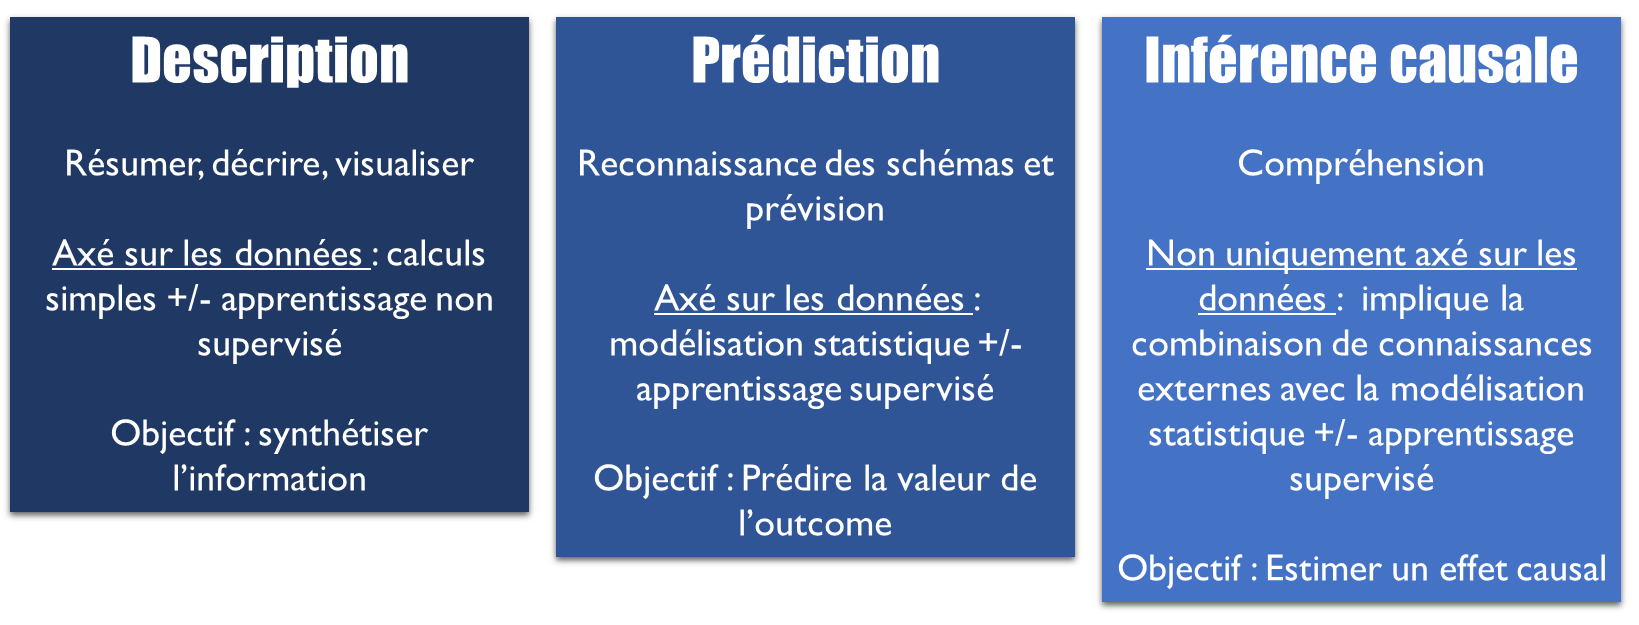
\includegraphics[width=1\textwidth,height=\textheight]{img/threetask.png}

Selon le type d'objectif, la démarche d'analyse et les enjeux méthodologiques ne vont pas être les mêmes. Si l'objectif est prédictif, la démarche va être centrée sur la \emph{prédiction de l'outcome}, à partir de covariables sélectionnées afin d'optimiser les performances de la prédiction, tout en prenant en compte leur disponibilité en pratique et la parcimonie du modèle.

Dans une démarche explicative, ou \emph{étiologique}, au contraire, la démarche va être centrée sur l'\emph{estimation d'un effet causal}, en prenant en compte les covariables en fonction de leur rôle vis-à-vis de l'effet d'intérêt (facteurs de confusion, colliders, médiateurs\ldots).

En épidémiologie, à l'exception des cas où l'on souhaite développer un test ou score diagnostique ou pronostique, les objectifs sont le plus souvent explicatifs. On cherche en effet, la plupart du temps, à identifier des liens de cause à effet, afin de pouvoir agir sur les causes pour modifier les effets.

Finalement, pour répondre à la question ``quand doit-on prendre en compte les interactions ?'', il est d'abord nécessaire d'identifier dans quel type de démarche l'on s'inscrit :

\begin{itemize}
\tightlist
\item
  \textbf{Démarche prédictive} : on ajoutera alors les interactions dans le modèle de prédiction, pour le rendre plus \emph{flexible}, si cela améliore les performances de la prédiction \citet{vanderweele_tutorial_2014}.
\item
  \textbf{Démarche explicative/étiologique} : on étudiera les interactions ou modifications d'effet, si cela répond directement à l'objectif. Par exemple :

  \begin{itemize}
  \tightlist
  \item
    Si l'objectif est du type ``l'effet de \(X\) sur \(Y\) varie-t-il en fonction de \(V\) ?'', on prendra en compte l'interaction entre \(X\) et \(V\).
  \item
    Les objectifs qui nécessitent la prise en compte de l'interaction peuvent aussi être du type : ``Quel est l'effet conjoint de \(X\) et \(V\) sur \(Y\) ?'' ou ``Quel part de l'effet de \(X\) sur \(Y\) disparaît quand \(V\) est modifié ?'', etc.
  \item
    Par contre, si l'objectif est simplement d'estimer l'effet de \(X\) sur \(Y\), ou l'effet médié par un médiateur \(M\), la prise en compte des interactions entre \(X\) et des covariables (facteurs de confusion ou médiateurs) n'est pas indispensable pour répondre à la question scientifique. Un effet ``moyen'' pourra être estimé. Des termes d'interactions peuvent cependant être ajoutés (mais non interprétés), si cela améliore la précision de l'estimation (enjeu d'optimisation du modèle).
  \end{itemize}
\end{itemize}

\hypertarget{types-dobjectifs}{%
\subsection{Types d'objectifs}\label{types-dobjectifs}}

Dans ce document, nous nous intéresserons principalement aux interactions et modifications d'effet dans une démarche étiologique/ explicative.

Les objectifs pouvant nécessiter l'étude de l'interaction/modification d'effet sont \citet{vanderweele_tutorial_2014} :

\begin{itemize}
\tightlist
\item
  \textbf{Cibler des sous-groupes}. Par exemple, identifier des sous-groupes pour lesquels l'intervention aura le plus d'effet afin de pouvoir cibler l'intervention en cas de ressources limitées, ou s'assurer que l'intervention est bénéfique pour tous les groupes et pas délétères pour certains groupes.
\item
  \textbf{Explorer les mécanismes d'un effet}. Par exemple, en cas d'intervention qui n'a d'effet qu'en présence ou absence d'une caractéristiques particulière (définition mécanistique de l'interaction) ou seulement conjointement à une autre intervention.
\item
  \textbf{Etudier l'effet d'une intervention pour éliminer une partie de l'effet d'une exposition non modifiable}. Par exemple, quelle part de l'effet du niveau d'éducation des parents sur la mortalité disparaîtrait si on intervenait sur le tabagisme à l'adolescence ? Ce type d'objectif est proche d'un objectif ciblant la \emph{médiation} d'un effet, par exemple la médiation de l'effet du niveau d'éducation des parents \emph{par} le tabagisme, mais les mécanismes envisagés et explorés ne sont pas exactement les mêmes. Explorer ces deux types de mécanismes peut nécessiter des approches spécifiques (voir chapitre \ref{plusloin})
\end{itemize}

\hypertarget{les-points-les-plus-importants}{%
\section{Les points les plus importants}\label{les-points-les-plus-importants}}

La première étape importante consiste donc à \textbf{définir précisément l'objectif} :

\begin{itemize}
\tightlist
\item
  L'objectif est-il de type descriptif, prédictif ou explicatif ?
\item
  Si l'on est dans une démarche explicative, d'inférence causale, est-ce que la mesure d'un effet d'interaction est nécessaire pour y répondre ? (identifier précisément l'effet que l'on cherche à estimer, ou \emph{estimand}).
\end{itemize}

Ensuite, de \textbf{nombreuses questions} se posent pour réaliser une analyse d'interaction, auxquelles nous tentons de répondre dans ce document :

\begin{itemize}
\tightlist
\item
  S'agit-il d'une interaction ou une modification d'effet ? (Chapitre \ref{intmodif})
\item
  Sur quelle échelle la mesure-t-on ? Un effet d'interaction peut en effet être défini sur une échelle multiplicative ou additive, et les résultats entre ces échelles peuvent être contradictoires. (Chapitre \ref{echelle})
\item
  Quels paramètres présenter et comment les interpréter ? (Chapitre \ref{param})
\item
  Comment estimer ces paramètres ? (Chapitre \ref{regression} et Chapitre \ref{conf})
\item
  Comment représenter cette interaction graphiquement ? (Chapitre \ref{graph})
\end{itemize}

\hypertarget{avertissements}{%
\section{Avertissements}\label{avertissements}}

\textbf{Puissance/sample size}

\hypertarget{part-synthuxe8se-de-la-littuxe9rature}{%
\part{Synthèse de la littérature}\label{part-synthuxe8se-de-la-littuxe9rature}}

\hypertarget{duxe9finitions-pruxe9alables}{%
\chapter{Définitions préalables}\label{duxe9finitions-pruxe9alables}}

\hypertarget{variables-et-probabilituxe9s}{%
\section{Variables et probabilités}\label{variables-et-probabilituxe9s}}

On note :

\begin{itemize}
\tightlist
\item
  un outcome : \(\small Y\),
\item
  deux expositions : \(\small X\) et \(\small V\)
\end{itemize}

La probabilité de l'outcome \(\small Y\) dans chaque strate définie par les 2 expositions est notée :

\begin{itemize}
\tightlist
\item
  \(\small p_{xv} = P(Y = 1|X = x,V = v)\)
\end{itemize}

\begin{quote}
Exemple

On a deux expositions \(\small X\), le tabagisme actif à 20 ans, et \(\small V\), le fait d'avoir vécu un évènement traumatique pendant l'enfance. L'outcome \(\small Y\) est binaire et représente le fait d'avoir au moins une pathologie chronique à 60 ans (\(\small Y=1\)) ou aucune (\(\small Y=0\)).

On décrit (données complètement fictives) :

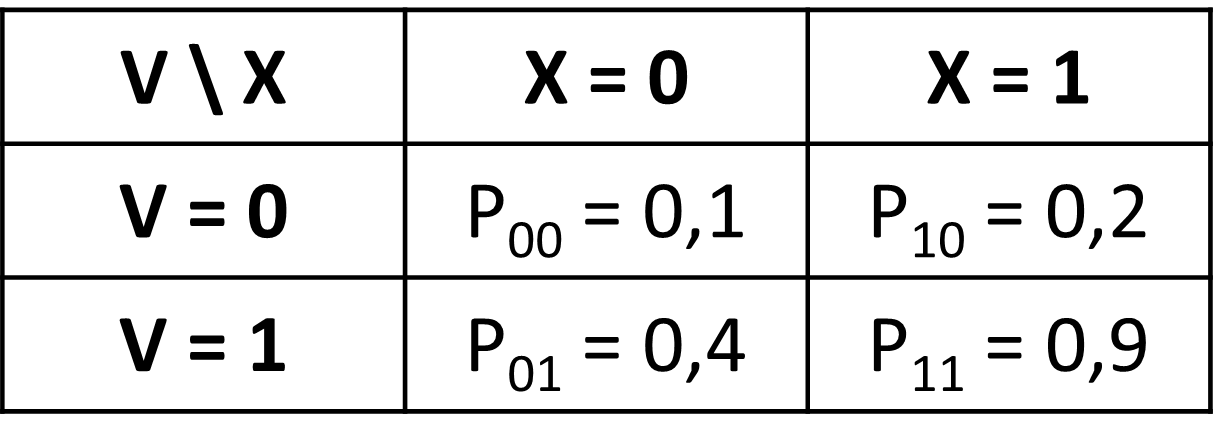
\includegraphics[width=0.4\textwidth,height=\textheight]{img/Image1.png}

Interprétation : La probabilité d'avoir au moins une pathologie chronique à 60 ans quand on n'a pas vécu d'événement traumatique pendant l'enfance et pas fumé à 20 ans est de 10\%, tandis qu'elle est de 90\% quand on a vécu un événement traumatique et fumé.
\end{quote}

\hypertarget{mesures-deffets}{%
\section{Mesures d'effets}\label{mesures-deffets}}

L'effet d'une variable \(\small X\) sur \(\small Y\) peut être mesuré sur deux échelles : additive (différence de risques ou de probabilités) ou multiplicative (rapport de risques ou de probabilités).

\hypertarget{concernant-les-diffuxe9rences-de-risques-dr-effets-additifs}{%
\subsection*{Concernant les différences de risques (DR, effets additifs)}\label{concernant-les-diffuxe9rences-de-risques-dr-effets-additifs}}
\addcontentsline{toc}{subsection}{Concernant les différences de risques (DR, effets additifs)}

On va noter \(\small P(Y = 1|do(X = 1))\) la probabilité d'observer \(\small Y=1\) sous une intervention contrefactuelle où la totalité de la population étudiée est exposée à \(\small X=1\) (notée \(\small do(X=1)\)).

De même, on va noter \(\small P(Y = 1|do(X=1,V=1))\) la probabilité d'observer \(\small Y=1\) sous une intervention contrefactuelle conjointe à la fois sur \(\small X\) et sur \(\small V\) où la totalité de la population étudiée est exposée à \(\small X=1\) et \(\small V=1\) (notée \(\small do(X=1,V=1)\)).

\begin{itemize}
\tightlist
\item
  L'effet d'une exposition \(X\) binaire sur \(Y\) est : \(\small DR(X) = P(Y = 1|do(X = 1)) - P(Y = 1|do(X = 0))\)

  \begin{itemize}
  \tightlist
  \item
    qu'on peut estimer, si les conditions d'identifiabilité sont réunies,
  \item
    par \(\small P(Y = 1|X = 1) - P(Y = 1|X = 0) = p_1-p_0\)
  \end{itemize}
\item
  L'effet conjoint de \(\small X\) et \(\small V\) est : \(\small DR(X,V) = p_{11}-p_{00}\)
\item
  L'effet de \(\small X\) sur \(\small Y\) pour chaque valeur fixée de \(\small V\) est : \(\small DR(X,V=0) = p_{10}-p_{00}\) et \(\small DR(X,V=1) = p_{11}-p_{01}\)
\end{itemize}

\begin{quote}
Exemple

Différences de risques pour l'exemple 1

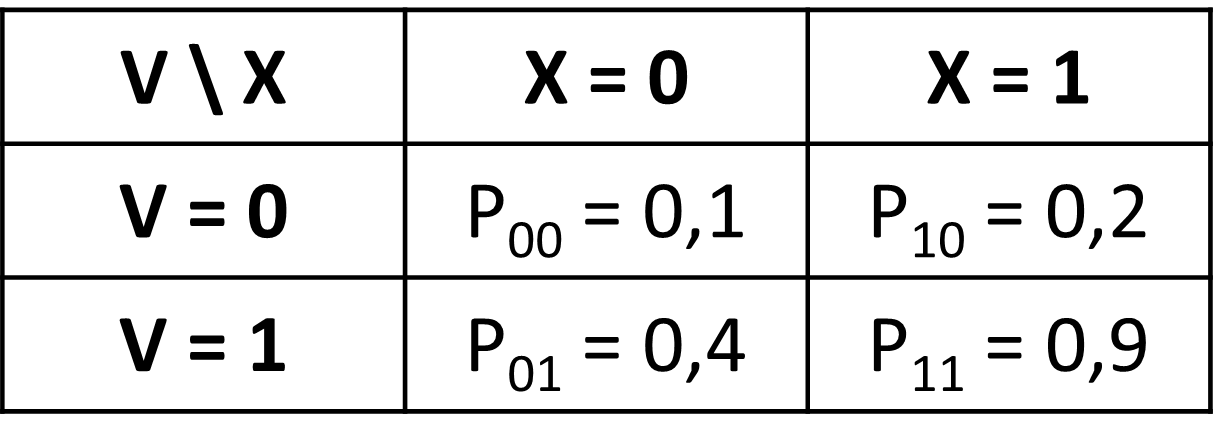
\includegraphics[width=0.3\textwidth,height=\textheight]{img/Image1.png}

\begin{itemize}
\tightlist
\item
  \(\small DR(X,V) = p_{11}-p_{00} = 0,90 - 0,10 = +0,80\)
\item
  \(\small DR (X,V=0) = p_{10}-p_{00} = 0,40 - 0,10 = +0,30\)
\item
  \(\small DR (X,V=1) = p_{11}-p_{01} = 0,90 - 0,20 = +0,70\)
\end{itemize}

Le fait d'être doublement exposé (tabagisme + événement traumatique) par rapport à pas du tout augmente le risque d'avoir au moins une pathologie chronique à 60 ans de +80\%. Dans une population n'ayant pas vécu d'événement traumatique, le fait de fumer à 20 ans augmente le risque d'avoir au moins une pathologie chronique à 60 ans de +30\%, alors que dans une population ayant vécu un événement traumatique, il est augmenté de +70\%.
\end{quote}

\hypertarget{concernant-les-rapports-de-risques-effets-multiplicatifs}{%
\subsection*{Concernant, les rapports de risques (effets multiplicatifs)}\label{concernant-les-rapports-de-risques-effets-multiplicatifs}}
\addcontentsline{toc}{subsection}{Concernant, les rapports de risques (effets multiplicatifs)}

on peut notamment utiliser les \textbf{risques relatifs} (RR). On donc :

\begin{itemize}
\tightlist
\item
  L'effet d'une exposition \(\small X\) binaire sur \(\small Y\) est :

  \begin{itemize}
  \tightlist
  \item
    \(\small RR(X) = \frac{P(Y = 1| do(X = 1)) }{ P(Y = 1|do(X = 0))}\)
  \item
    qu'on peut estimer, si les conditions d'identifiabilité sont réunies, par :
  \item
    \(\small \frac{P(Y = 1| do(X = 1)) }{ P(Y = 1|do(X = 0))} = \frac{p_1}{p_0}\)
  \end{itemize}
\item
  L'effet conjoint de \(\small X\) et \(\small V\) est : \(\small RR(X,V) = \frac{p_{11}}{p_{00}}\)
\item
  L'effet de \(\small X\) sur \(\small Y\) pour chaque valeur fixée de \(\small V\) est :

  \begin{itemize}
  \tightlist
  \item
    \(\small RR(X,V=0) = \frac{p_{10}}{p_{00}}\)
  \item
    et \(\small RR(X,V=1) = \frac{p_{11}}{p_{01}}\)
  \end{itemize}
\end{itemize}

\begin{quote}
Exemple

Risques relatifs pour l'exemple 1

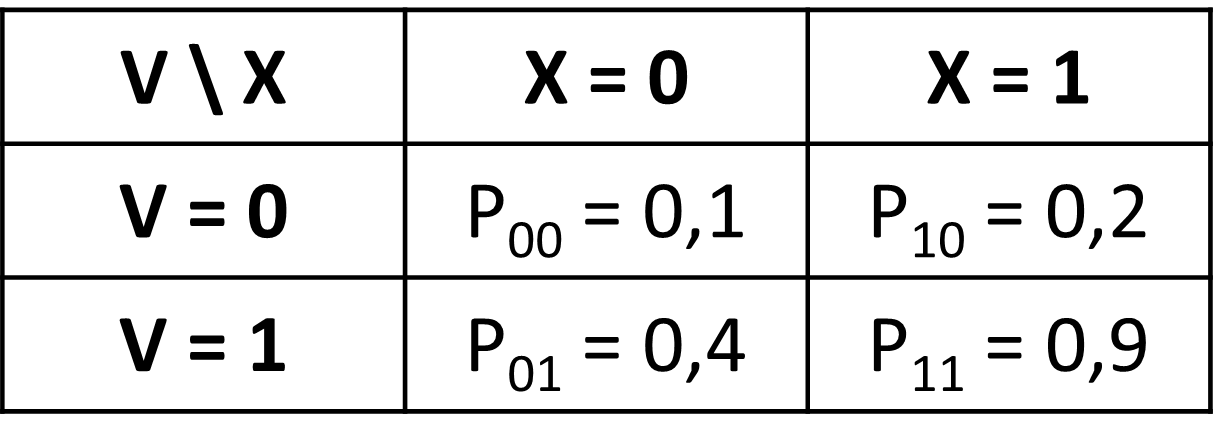
\includegraphics[width=0.3\textwidth,height=\textheight]{img/Image1.png}

\begin{itemize}
\tightlist
\item
  \(\small RR(X,V) = \frac{0,9}{0,1} = \times 9\)
\item
  \(\small RR(X,V=0) = \frac{0,4}{0,1} = \times 4\)
\item
  \(\small RR(X,V=1) = \frac{0,9}{0,2} = \times 4,5\)
\end{itemize}

Le risque d'avoir au moins une pathologie chronique à 60 ans quand on est doublement exposé (tabagisme + événement traumatique) par rapport à pas du tout est multiplié par 9. Dans une population n'ayant pas vécu d'événement traumatique, le fait de fumer à 20 ans multiplie le risque par 4, alors que dans une population ayant vécu un événement traumatique, il est multiplié par 4,5.
\end{quote}

\hypertarget{effets-conditionnels-et-marginaux}{%
\section{Effets conditionnels et marginaux}\label{effets-conditionnels-et-marginaux}}

\textbf{A compléter}

\hypertarget{intmodif}{%
\chapter{Interaction ou modification d'effets}\label{intmodif}}

Dans le champ des analyses d'interaction, deux termes peuvent être rencontrés : ``interaction'' et ``modification d'effet''. Quel est la différence entre ces deux termes ?

\hypertarget{modification-deffets}{%
\section{Modification d'effets}\label{modification-deffets}}

La question de la modification d'effet consiste à identifier si un scénario contrefactuel modifiant le traitement ou l'exposition \(\small X\) donne un résultat différent dans différents groupes \(\small V\) de patients (estimer l'effet d'une exposition séparément en fonction d'une autre variable) \citet{corraini_effect_2017}.

Si l'on compare avec un essai d'intervention, c'est comme s'il y avait une seule intervention \(\small X\) et que l'analyse était stratifiée sur \(\small V\). On analyse donc l'effet du scénario \(\small do(X)\) dans chaque groupe de \(\small V\).

En observationnel, l'effet causal qui nous intéresse est donc celui de \(\small X\) mais pas celui de \(\small V\).
On ajustera sur les facteurs de confusion de la relation \(\small X \rightarrow Y\).

On ne fait pas d'hypothèse sur les mécanismes de la modification d'effet, qui peut être causale (de façon directe ou indirecte), ou non-causale (présence d'une modification d'effet par proxy ou cause commune, sans qu'il existe d'effet direct ou indirect du modificateur d'effet vers le critère de jugement, comme dans la figure en bas de page) \citet{vanderweele_four_2007}.

\begin{quote}
Exemples d'objectifs : identifier des groupes pour lesquels le traitement ne serait pas utile, ou explorer si l'effet du traitement est homogène/hétérogène en fonction de l'âge, du sexe, etc.
\end{quote}

On a une modification de l'effet de \(\small X\) par \(\small V\) si l'effet de \(\small X\) est différent dans deux strates définies par \(\small V\):

\begin{itemize}
\tightlist
\item
  en additif : \(\small DR(X | V=0) \neq DR(X | V=1)\)

  \begin{itemize}
  \tightlist
  \item
    soit \(\small p_{10}-p_{00} \neq p_{11}-p_{01}\)\\
  \end{itemize}
\item
  en multiplicatif : \(\small RR(X | V=0) \neq RR(X | V=1)\)

  \begin{itemize}
  \tightlist
  \item
    soit \(\small \frac{p_{10}}{p_{00}} \neq \frac{p_{11}}{p_{01}}\)
  \end{itemize}
\end{itemize}

\begin{quote}
Exemple

Modification d'effet dans l'exemple 1

En additif :

\begin{itemize}
\tightlist
\item
  effet dans le groupe \(\small V=0\) : \(\small DR (X | V=0) = 0,40 - 0,10 = +0,30\)
\item
  effet dans le groupe \(\small V=1\) : \(\small DR (X | V=1) = 0,90 - 0,20 = +0,70\)
\item
  donc \(\small DR (X | V=0) \neq DR (X | V=1)\)
\end{itemize}

En multiplicatif :

\begin{itemize}
\tightlist
\item
  effet dans le groupe \(\small V=0\) : \(\small RR(X | V=0) = \frac{0,40}{0,10} = \times 4,0\)
\item
  effet dans le groupe \(\small V=1\) : \(\small RR(X | V=1) = \frac{0,90}{0,20} = \times 4,5\)
\item
  donc \(\small RR(X | V=0) \neq RR(X | V=1)\)
\end{itemize}

Ici l'effet du tabagisme est différent selon que les personnes ont vécu un événement traumatique ou non, sur l'échelle additive et multiplicative (données fictives). On peut donc dire que le fait d'avoir vécu un événement traumatique modifie l'effet du tabac. Attention, dans cet exemple, on fait l'hypothèse de l'absence de facteurs de confusion entre le tabagisme et l'outcome, ce qui est en réalité peu probable.
\end{quote}

Lorsqu'on utilise les approches causales pour estimer l'effet de \(\small X\) sur \(\small Y\), on va intervenir seulement sur X. En G-computation, le code serait :

\hypertarget{interaction}{%
\section{Interaction}\label{interaction}}

Quand on s'intéresse à l'interaction, on s'intéresse plutôt à l'effet conjoint de 2 expositions (ou plus) sur un outcome. Il y a une interaction synergique si l'effet conjoint est supérieur à la somme de l'effet individuels. Il y a une interaction antagoniste lorsque l'effet conjoint est inférieur à la somme des effets individuels \citet{corraini_effect_2017}.

Si l'on compare avec un essai d'intervention, c'est comme s'il y avait plusieurs interventions, selon le nombre de combinaisons. On analyse donc l'effet du scénario \(\small do(X, V)\). Ici l'effet causal d'intérêt est vraiment l'effet conjoint des deux variables.

Dans un schéma observationnel, l'effet causal qui nous intéresse est donc celui de l'interaction \(\small X*V\). On ajustera sur les facteurs de confusion des deux relations \(\small X \rightarrow Y\) et \(\small V \rightarrow Y\).
On fait l'hypothèse que les mécanismes de l'effet conjoint de \(\small X\) et \(\small V\) sont causaux.

Par définition, on a une interaction si l'effet conjoint de \(\small X\) et \(\small V\) sur \(\small Y\) (\(\small DR(X,V)\)) est différent de la somme (ou du produit sur l'échelle multiplicative) :

\begin{itemize}
\tightlist
\item
  de l'effet isolé de \(\small X\) sur \(\small Y\) (où \(\small V\) est constant, fixé à \(\small V=0\)), noté \(\small DR(X,V=0)\) (ou \(\small RR(X,V=0)\))
\item
  et de l'effet isolé de \(\small V\) sur \(\small Y\) (où \(\small X\) est constant, fixé à \(\small X=0\)), noté \(\small DR(V,X=0)\) (ou \(\small RR(V,X=0)\))
\end{itemize}

On a ainsi,

\begin{itemize}
\tightlist
\item
  en additif : \(\small DR(X,V) \neq DR(X,V=0) + DR(V,X=0)\)

  \begin{itemize}
  \tightlist
  \item
    \(\small p_{11}-p_{00} \neq (p_{10}-p_{00})+(p_{01}-p_{00})\)
  \item
    \(\small p_{11} \neq p_{10} + p_{01} - p_{00}\)
  \item
    \(\small p_{11} - p_{10} - p_{01} + p_{00} \neq 0\)
  \end{itemize}
\item
  en multiplicatif \(\small RR(X,V) \neq RR(X,V=0) \times RR(V,X=0)\)

  \begin{itemize}
  \tightlist
  \item
    \(\small \frac{p_{11}}{p_{00}} \neq \frac{p_{10}}{p_{00}} \times \frac{p_{01}}{p_{00}}\)
  \item
    \(\small p_{11} \neq \frac{\frac{p_{10}}{p_{01}}}{p_{00}}\)
  \item
    \(\small \frac{p_{00} \times p_{11}}{p_{10} \times p_{01}} \neq 1\)
  \end{itemize}
\end{itemize}

\begin{quote}
Exemple

Interaction dans l'exemple 1

En additif :

\begin{itemize}
\tightlist
\item
  effet joint : \(\small DR(X,V) = 0,90 - 0,10 = +0.80\)
\item
  somme des effets individuels : \(\small DR(X,V=0) + DR(V,X=0) = +0,30 +0,10 = +0,40\)
\item
  donc \(\small DR(X,V) \neq DR(X,V=0) + DR(V,X=0)\)
\end{itemize}

En multiplicatif :

\begin{itemize}
\tightlist
\item
  effet joint : \(\small RR(X,V) = \frac{0,9}{0,1} = \times 9\)
\item
  produit des effets individuels : \(\small RR(X,V=0) \times RR(V,X=0) = 4 \times 2 = \times 8\)
\item
  donc \(\small DR(X,V) \neq DR(X,V=0) \times DR(V,X=0)\)
\end{itemize}

Ici l'effet joint des 2 expositions est supérieur à la somme ou au produit des effets individuels, il y a donc une interaction synergique entre les deux expositions. On peut conclure que l'expérience d'un événement traumatique et le tabagisme se potentialise pour aboutir à une augmentation du risque de maladies chroniques : ces expositions ont un effet plus fort lorsqu'elles sont présentes toutes les deux.
\end{quote}

Lorsqu'on utilise les approches causales pour estimer l'effet de \(\small X\) sur \(\small Y\), on va intervenir seulement sur X. En G-computation, le code serait :

\begin{Shaded}
\begin{Highlighting}[]
       \CommentTok{\#modèle}
\NormalTok{       Q.model }\OtherTok{\textless{}{-}} \FunctionTok{glm}\NormalTok{(}\AttributeTok{data=}\NormalTok{bootData, }\AttributeTok{formula =}\NormalTok{ Y }\SpecialCharTok{\textasciitilde{}}\NormalTok{ X }\SpecialCharTok{+}\NormalTok{ V }\SpecialCharTok{+}\NormalTok{ X}\SpecialCharTok{*}\NormalTok{V ,}\AttributeTok{family =}\NormalTok{ binomial)}
       
       \CommentTok{\# Scénarios \#}
\NormalTok{       data.X0V0 }\OtherTok{\textless{}{-}}\NormalTok{  data.X0V1 }\OtherTok{\textless{}{-}}\NormalTok{  data.X1V0 }\OtherTok{\textless{}{-}}\NormalTok{  data.X1V1 }\OtherTok{\textless{}{-}}\NormalTok{ bootData}
\NormalTok{       data.X0V0}\SpecialCharTok{$}\NormalTok{X }\OtherTok{\textless{}{-}}\NormalTok{  data.X0V1}\SpecialCharTok{$}\NormalTok{X }\OtherTok{\textless{}{-}} \DecValTok{0}
\NormalTok{       data.X1V0}\SpecialCharTok{$}\NormalTok{X }\OtherTok{\textless{}{-}}\NormalTok{  data.X1V1}\SpecialCharTok{$}\NormalTok{X }\OtherTok{\textless{}{-}} \DecValTok{1}
\NormalTok{       data.X0V0}\SpecialCharTok{$}\NormalTok{V }\OtherTok{\textless{}{-}}\NormalTok{  data.X1V0}\SpecialCharTok{$}\NormalTok{V }\OtherTok{\textless{}{-}} \DecValTok{0}
\NormalTok{       data.X0V1}\SpecialCharTok{$}\NormalTok{V }\OtherTok{\textless{}{-}}\NormalTok{  data.X1V1}\SpecialCharTok{$}\NormalTok{V }\OtherTok{\textless{}{-}} \DecValTok{1}

       \CommentTok{\# Y contrefactuel}
\NormalTok{       Y.X0V0.pred }\OtherTok{\textless{}{-}} \FunctionTok{predict}\NormalTok{(Q.model, }\AttributeTok{newdata =}\NormalTok{ data.X0V0, }\AttributeTok{type =} \StringTok{"response"}\NormalTok{)}
\NormalTok{       Y.X1V0.pred }\OtherTok{\textless{}{-}} \FunctionTok{predict}\NormalTok{(Q.model, }\AttributeTok{newdata =}\NormalTok{ data.X1V0, }\AttributeTok{type =} \StringTok{"response"}\NormalTok{)}
\NormalTok{       Y.X0V1.pred }\OtherTok{\textless{}{-}} \FunctionTok{predict}\NormalTok{(Q.model, }\AttributeTok{newdata =}\NormalTok{ data.X0V1, }\AttributeTok{type =} \StringTok{"response"}\NormalTok{)}
\NormalTok{       Y.X1V1.pred }\OtherTok{\textless{}{-}} \FunctionTok{predict}\NormalTok{(Q.model, }\AttributeTok{newdata =}\NormalTok{ data.X1V1, }\AttributeTok{type =} \StringTok{"response"}\NormalTok{)}
       
       \CommentTok{\# Interaction}

\NormalTok{         simu.base}\SpecialCharTok{$}\NormalTok{est.Y0\_30[simu.base}\SpecialCharTok{$}\NormalTok{i.simu}\SpecialCharTok{==}\NormalTok{i] }\OtherTok{=} \FunctionTok{round}\NormalTok{(}\FunctionTok{mean}\NormalTok{(Y.S2A30.pred),}\DecValTok{4}\NormalTok{)}
\end{Highlighting}
\end{Shaded}

\hypertarget{synthuxe8se}{%
\section{Synthèse}\label{synthuxe8se}}

Mathématiquement, les formulations sont équivalentes :

\begin{itemize}
\tightlist
\item
  échelle additive: \(\small p_{10} -p_{00} \neq p_{11}- p_{01} \iff p_{11} \neq (p_{10}+p_{01})- p_{00}\)
\item
  échelle multiplicative : \(\small p_{10} /p_{00} \neq p_{11}/ p_{01} \iff p_{11} \neq (p_{10} \times p_{01})/p_{00}\)
\end{itemize}

La différence se joue plutôt sur :

\begin{itemize}
\tightlist
\item
  la façon dont la question est posée (effet de \(\small X\) selon \(\small V\), \emph{versus} effet conjoint de \(\small X\) et \(\small V\)),
\item
  les hypothèses causales formulées (scénario \(\small do(X)|V\) \emph{versus} \(\small do(X,V)\))
\item
  et donc sur les sets de facteurs de confusion à considérer (seulement sur la relation \(\small X \rightarrow Y\) \emph{versus} les deux relations \(\small X \rightarrow Y\) et \(\small V \rightarrow Y\)).
\end{itemize}

Il existe des cas où l'identification d'une interaction ou d'une modification d'effet ne conduira pas à la même démarche et donc au même résultat \citet{vanderweele_distinction_2009}. Prenons le DAG suivant :

\begin{quote}
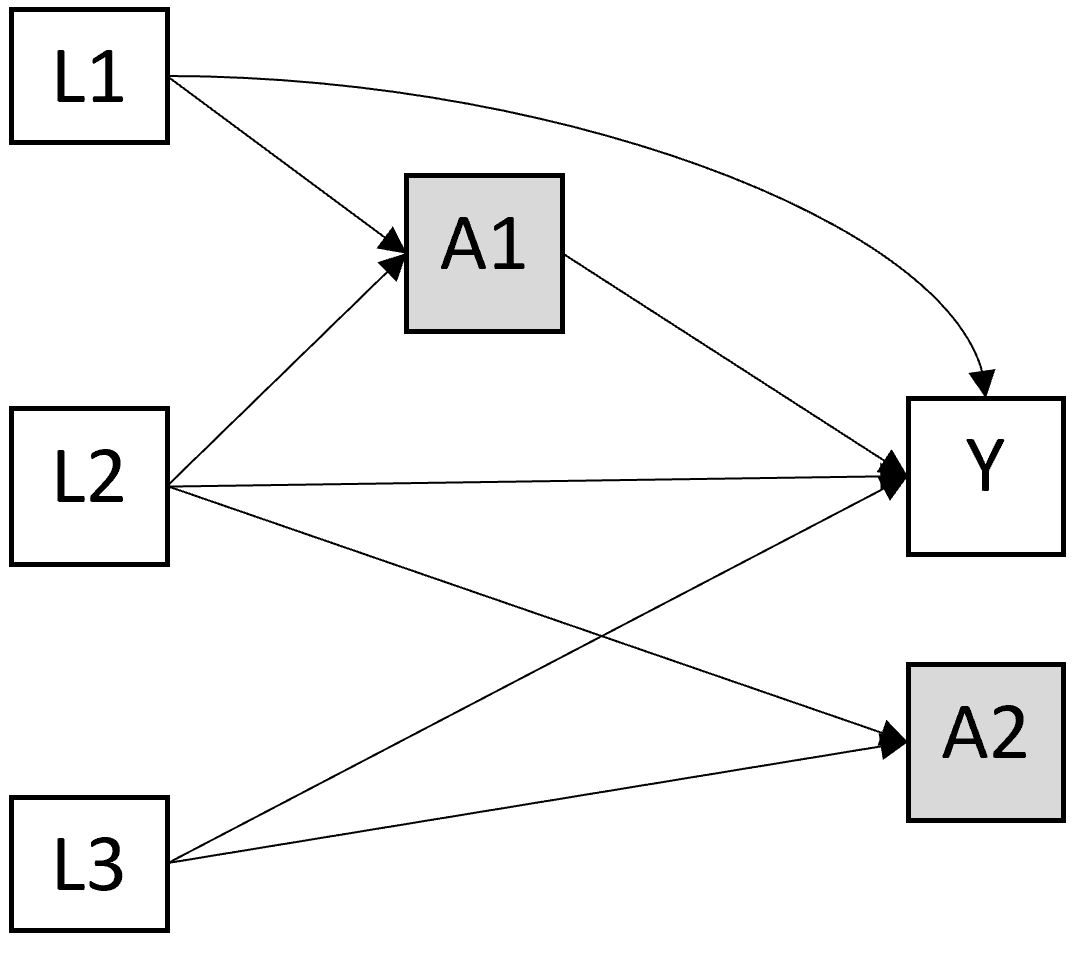
\includegraphics[width=0.3\textwidth,height=\textheight]{img/Image12.png}
\end{quote}

Dans ce cas, il n'y a pas d'interaction entre \(\small A1\) et \(\small A2\), car il n'y a pas d'effet direct ni indirect de \(\small A2 \rightarrow Y\). L'effet de \(\small A1 \rightarrow Y\) restera le même quelle que soit la valeur que l'on pourrait attribuer à \(\small A2\) :

\begin{multline*}
\scriptsize P\left[Y=1|do(A1=1, A2=0)\right] - P\left[Y=1|do(A1=0, A2=0)\right] = P\left[Y=1|do(A1=1, A2=1)\right] \\
\scriptsize - P\left[Y=1|do(A1=0, A2=1)\right]
\end{multline*}

Par contre, il peut y avoir une modification de l'effet de \(\small A1\) par \(\small A2\), en particulier s'il existe une interaction \(\small A1 * L2 \rightarrow Y\) ou \(\small A1 * L3 \rightarrow Y\), on s'attend à ce que les contrastes suivants soient différents :

\begin{multline*}
\scriptsize P[Y=1|do(A1=1),A2=1] - P[Y=1|do(A1=2),A2=1] \neq P[Y=1|do(A1=1),A2=0] \\
\scriptsize - P[Y=1|do(A1=2),A2=0]
\end{multline*}

\hypertarget{echelle}{%
\chapter{La question des échelles}\label{echelle}}

\hypertarget{mesures-des-interactions}{%
\section{Mesures des interactions}\label{mesures-des-interactions}}

\hypertarget{echelle-additive}{%
\subsection*{Echelle additive}\label{echelle-additive}}
\addcontentsline{toc}{subsection}{Echelle additive}

Une façon simple de mesurer l'interaction est de mesurer à quel point l'effet conjoint de deux facteurs est différents de la somme de leurs effets individuels \citet{vanderweele_tutorial_2014} :

\begin{itemize}
\tightlist
\item
  \(\small AI = DR(X,V) - [DR(X|V=0) + DR(V|X=0)]\)
\item
  \(\small AI = (p_{11} - p_{00}) - [(p_{10} - p_{00}) + (p_{01} - p_{00})]\)
\item
  soit \(\small AI =p_{11} - p_{10} - p_{01} + p_{00}\)
\end{itemize}

\begin{quote}
Exemple

Mesure de l'interaction dans l'exemple 1

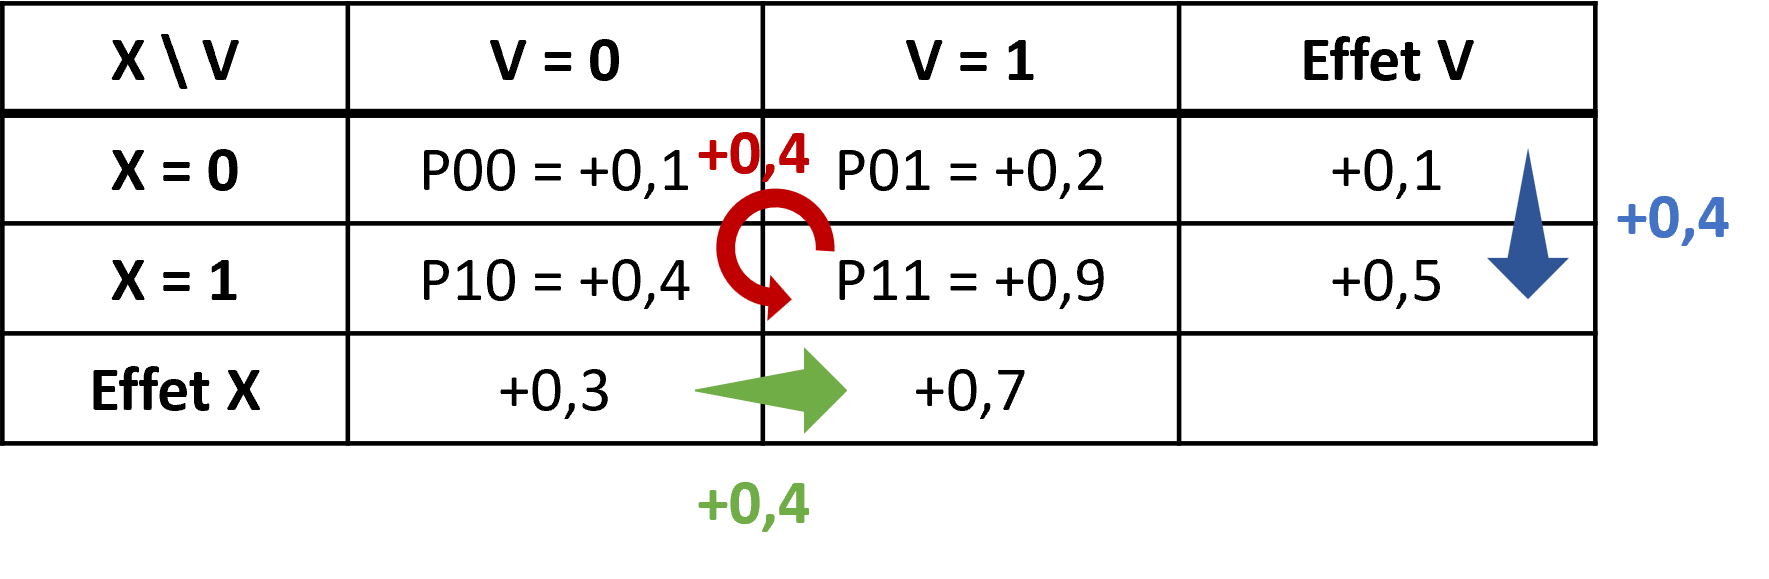
\includegraphics[width=0.65\textwidth,height=\textheight]{img/Image2.png}

On retrouve l'effet d'interaction, calculé/exprimé de différentes façon,

Soit :

\begin{itemize}
\tightlist
\item
  \(\small DR(X, V) - [DR(X|V=0) + DR(V|X=0)] = 0.8 - (0,3 + 0,1) = +0,4\)
\item
  \(\small p_{11} - p_{10} - p_{01} + p_{00} = 0,9 - 0,4 - 0,2 + 0,1 = +0,4\)
\item
  la différence entre l'effet joint et la somme des effets individuels (flèche rouge)
\end{itemize}

Soit :

\begin{itemize}
\tightlist
\item
  \(\small (p_{11} - p_{01}) - (p_{10} - p_{00}) = (0,9 - 0,2) - (0,4 - 0,1) = 0,7 - 0,3 = +0,4\)\\
\item
  la différence entre l'effet de X quand V = 1 et quand V = 0 (flèche verte)
\end{itemize}

Soit :

\begin{itemize}
\tightlist
\item
  \(\small (p_{11} - p_{10}) - (p_{01} - p_{00}) = (0,9 - 0,4) - (0,2 - 0,1) = 0,5 - 0,1 = +0,4\)\\
\item
  la différence entre l'effet de V quand X = 1 et quand X = 0 (flèche bleue)
\end{itemize}
\end{quote}

\hypertarget{echelle-multiplicative}{%
\subsection*{Echelle multiplicative}\label{echelle-multiplicative}}
\addcontentsline{toc}{subsection}{Echelle multiplicative}

En cas d'outcome binaire, c'est souvent le RR ou l'OR qui est utilisé pour mesurer les effets. La mesure de l'interaction sur une échelle multiplicative serait donc \citet{vanderweele_tutorial_2014} :

\begin{itemize}
\tightlist
\item
  \(\small MI = \frac{RR_{11}}{RR_{10} \times RR_{01}}\)
\item
  soit \(\small MI = \frac{p_{11} / p_{00}}{(p_{10} / p_{00}) \times (p_{01} / p_{00})}\)
\item
  soit \(\small MI = \frac{p_{11} \times p_{00}}{p_{10} \times p_{01}}\)
\end{itemize}

\begin{quote}
Exemple

Mesure de l'nteraction dans l'exemple 1

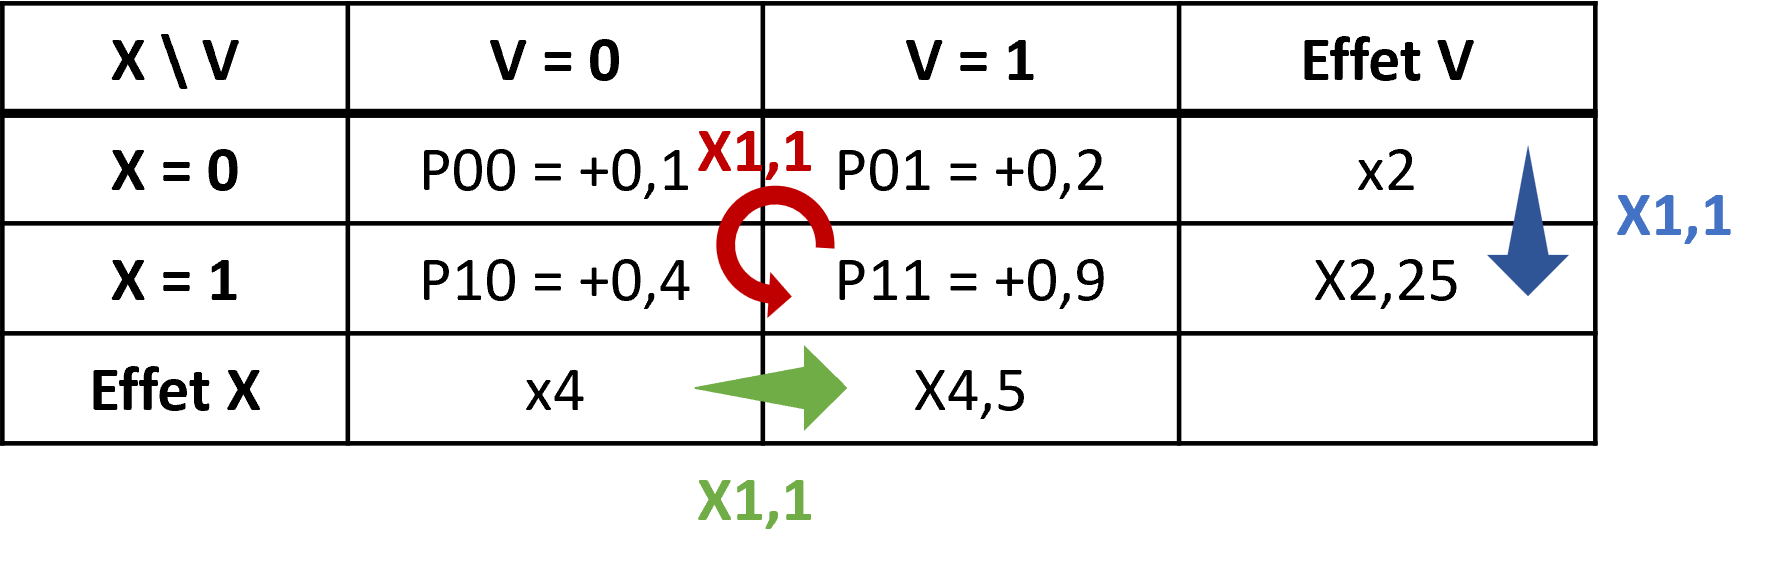
\includegraphics[width=0.65\textwidth,height=\textheight]{img/Image3.png}

On retrouve l'effet d'interaction, calculé/exprimé de différentes façon,

Soit :

\begin{itemize}
\tightlist
\item
  \(\small \frac{RR(X, V)}{RR(X| V=0)*RR(V|X=0)} = \frac{9}{4 \times 2} = \times 1,1\)
\item
  \(\small\frac{p_{11} / p_{00}}{(p_{10} + p_{01}) / p_{00}} = \frac{0,9 / 0,1}{(0,4 \times 0,2) / 0,1} = \times 1,1\)
\item
  le rapport entre l'effet joint et le produit des effets individuels (flèche rouge)
\end{itemize}

Soit :

\begin{itemize}
\tightlist
\item
  \(\small \frac{p_{11} / p_{01}}{p_{10} / p_{00}} = \frac{0,9 / 0,2}{0,4 / 0,1} = \frac{\times 4,5 }{\times 4} = \times 1,1\)
\item
  le produit de l'effet de X quand V = 1 et quand V = 0 (flèche verte)
\end{itemize}

Soit :

\begin{itemize}
\tightlist
\item
  ou \(\small \frac{p_{11} / p_{10}}{p_{01} / p_{00}} = \frac{0,9 / 0,4}{0,2 / 0,1} = \frac{\times 2,25}{\times 2} = \times 1,1\)
\item
  le produit de l'effet de V quand X = 1 et quand X = 0 (flèche bleue)
\end{itemize}
\end{quote}

\hypertarget{lien-entre-les-deux-uxe9chelles}{%
\section{Lien entre les deux échelles}\label{lien-entre-les-deux-uxe9chelles}}

\hypertarget{un-apparent-paradoxe}{%
\subsection*{Un apparent paradoxe}\label{un-apparent-paradoxe}}
\addcontentsline{toc}{subsection}{Un apparent paradoxe}

Mesurer l'interaction sur une seule échelle peut être trompeur \citet{mathur2018r}. On peut régulièrement observer une interaction positive dans une échelle (par exemple \(\small p11 - p10 - p01 + p00 > 0\)) et négative dans l'autre (par exemple \(\small (p11 \times p00) / (p10 \times p01) <1\)).

\begin{quote}
Exemple

Dans cet exemple (on modifie seulement la probabilité \(\small p_{11}\), en jaune dans le tableau), on observe une interaction additive positive (l'effet de \(\small X\) augmente de +20\% quand \(\small V=1\) par rapport à \(\small V=0\)) mais une interaction multiplicative négative (l'effet de \(\small X\) est multiplié par 0,9 - donc diminue - quand \(\small V=1\) par rapport à \(\small V=0\)).

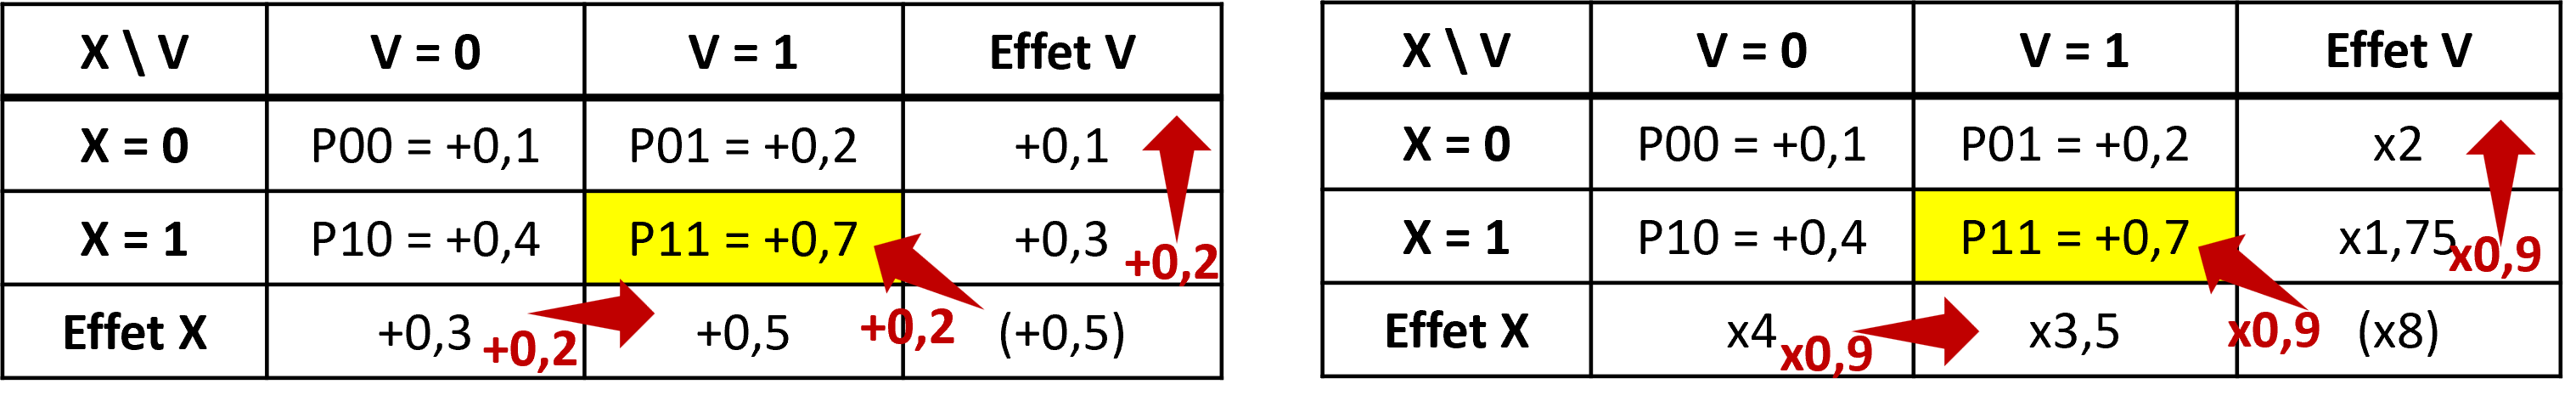
\includegraphics[width=0.9\textwidth,height=\textheight]{img/Image4.png}

\emph{Remarque : on retrouverait les mêmes résultats en comparant les effets de V dans les strates de X ou les effets conjoints et somme/produit des effets individuels.}
\end{quote}

Il a même été démontré que si on n'observe pas d'interaction sur une échelle, alors on en observera obligatoirement sur l'autre échelle\ldots{} \citet{vanderweele_tutorial_2014}.

\begin{quote}
Exemple

Dans cet exemple, il n'y a pas d'interaction multiplicative (effet de \(\small X\) identique quelque soit \(\small V\)), mais sur l'echelle additive, on observe une interaction positive.

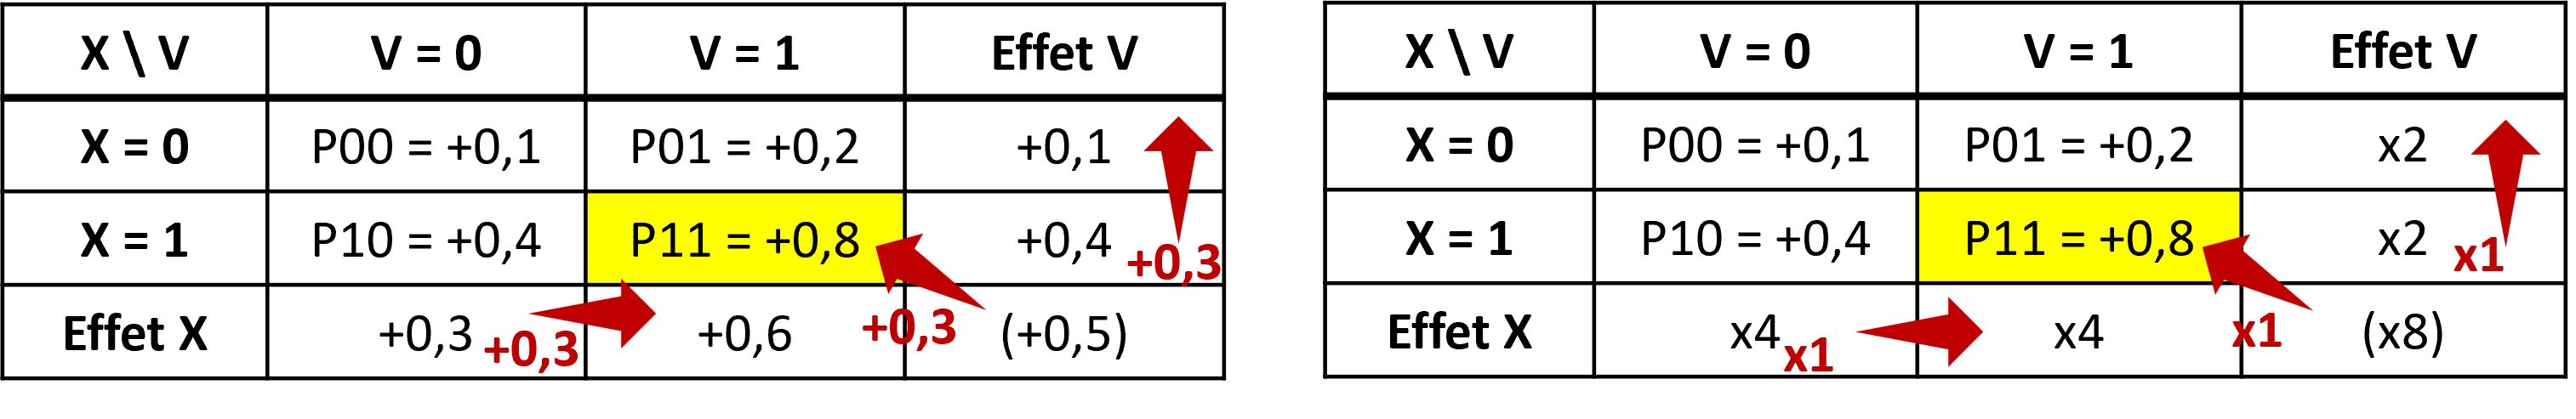
\includegraphics[width=0.9\textwidth,height=\textheight]{img/Image5.png}

Dans cet autre exemple, il n'y a pas d'interaction additive (effet de \(\small X\) identique quelque soit \(\small V\)), mais sur l'echelle multiplicative, on observe une interaction négative.

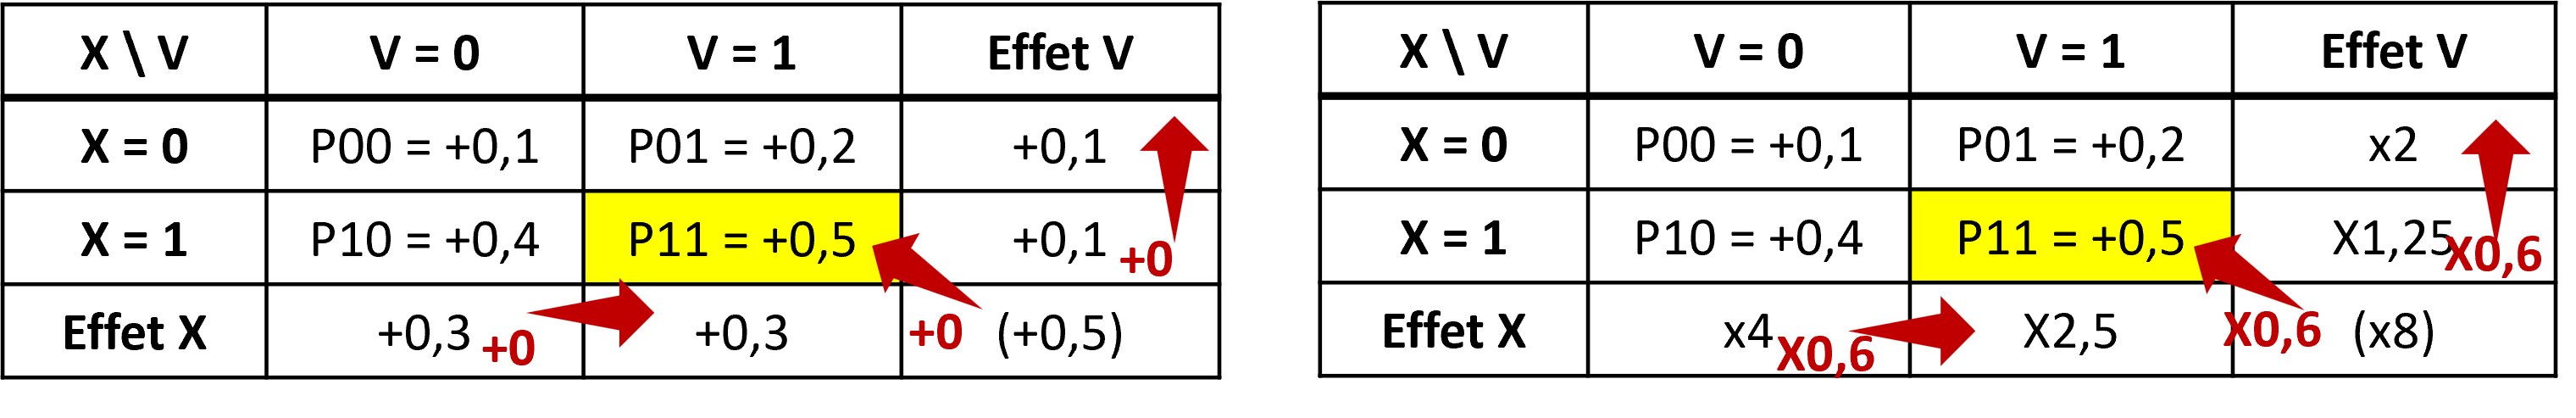
\includegraphics[width=0.9\textwidth,height=\textheight]{img/Image5b.png}
\end{quote}

\hypertarget{le-continuum}{%
\subsection*{Le continuum}\label{le-continuum}}
\addcontentsline{toc}{subsection}{Le continuum}

Dans un article de 2019 \citet{vanderweele_interaction_2019}, Vanderweele décrit le continuum existant entre les 2 échelles.

\begin{quote}
Par exemple, dans l'exemple 1, l'interaction additive et multiplicative sont positives. Mais si l'on fait varier la probabilité \(\small p_{11}\) en la diminuant, l'interaction multiplicative devient négative alors que l'interaction additive reste positive. Puis, lorsque la probabilité diminue encore, l'interaction devient négative sur les deux échelles :

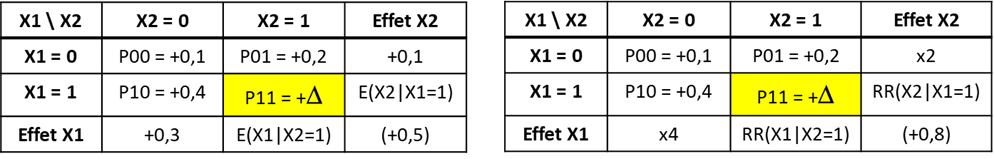
\includegraphics[width=1\textwidth,height=\textheight]{img/Image6.png}
\end{quote}

\hypertarget{interactions-pures-et-qualitatives-interactions-inversuxe9es}{%
\subsection*{Interactions pures et qualitatives, interactions inversées}\label{interactions-pures-et-qualitatives-interactions-inversuxe9es}}
\addcontentsline{toc}{subsection}{Interactions pures et qualitatives, interactions inversées}

Dans ce continuum, si l'on continue à faire varier \(\small p_{11}\), des cas particuliers d'interaction peuvent être retrouvés :

\begin{quote}
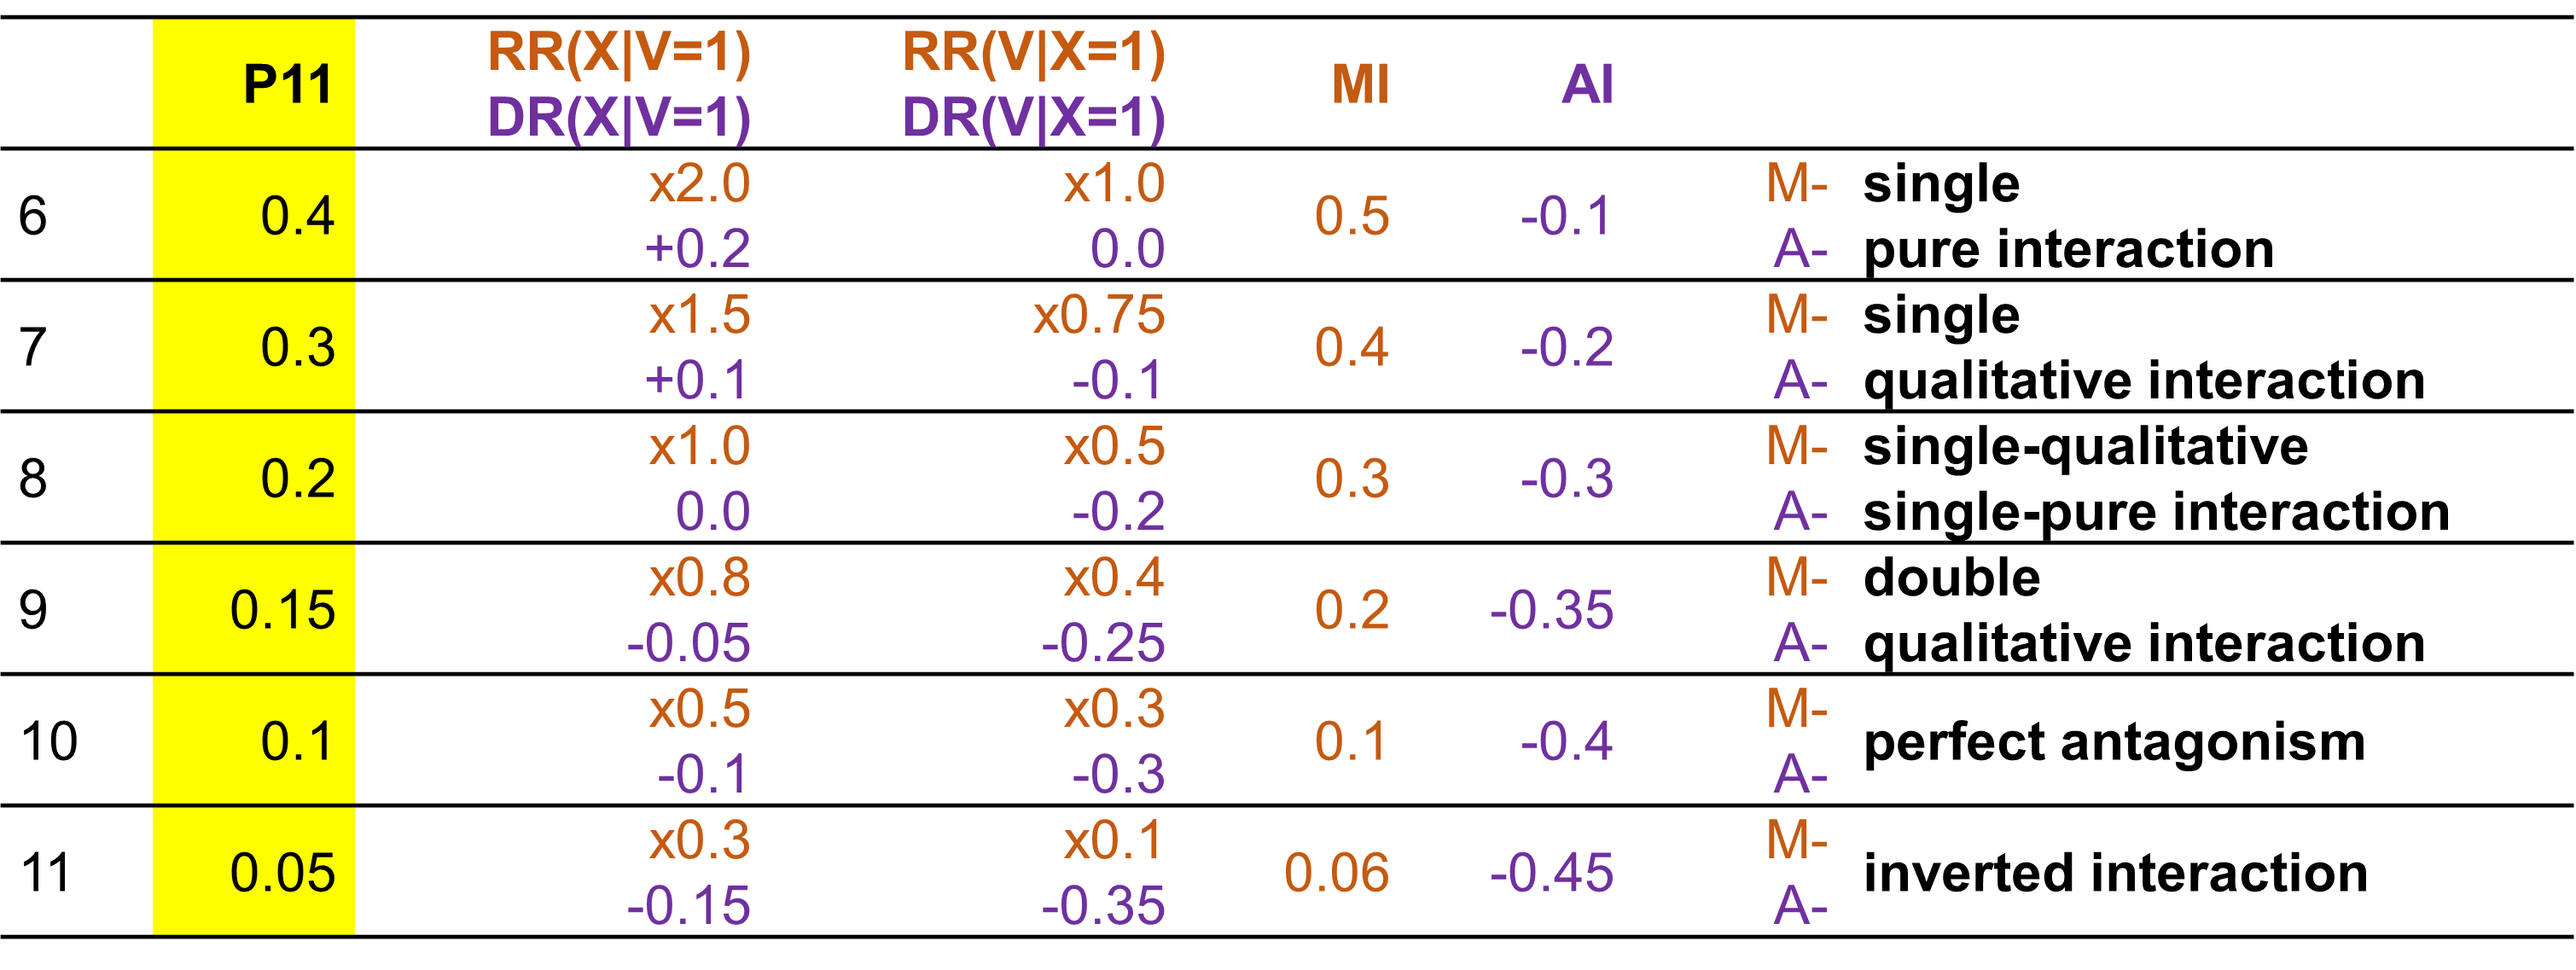
\includegraphics[width=1\textwidth,height=\textheight]{img/Image7.png}
\end{quote}

\begin{itemize}
\tightlist
\item
  \textbf{Interaction pure} de \(\small X\) en fonction de \(\small V\), si \(\small X\) n'a un effet que dans une seule strate de \(\small V\). Par exemple, \(\small p_{10} = p_{00}\) et \(\small p_{11} \neq p_{01}\).
\end{itemize}

\begin{quote}
Par exemple (ligne 6) ici, \(\small V\) a un effet (sur les deux échelles) si \(\small X=0\) mais pas si \(\small X=1\) :

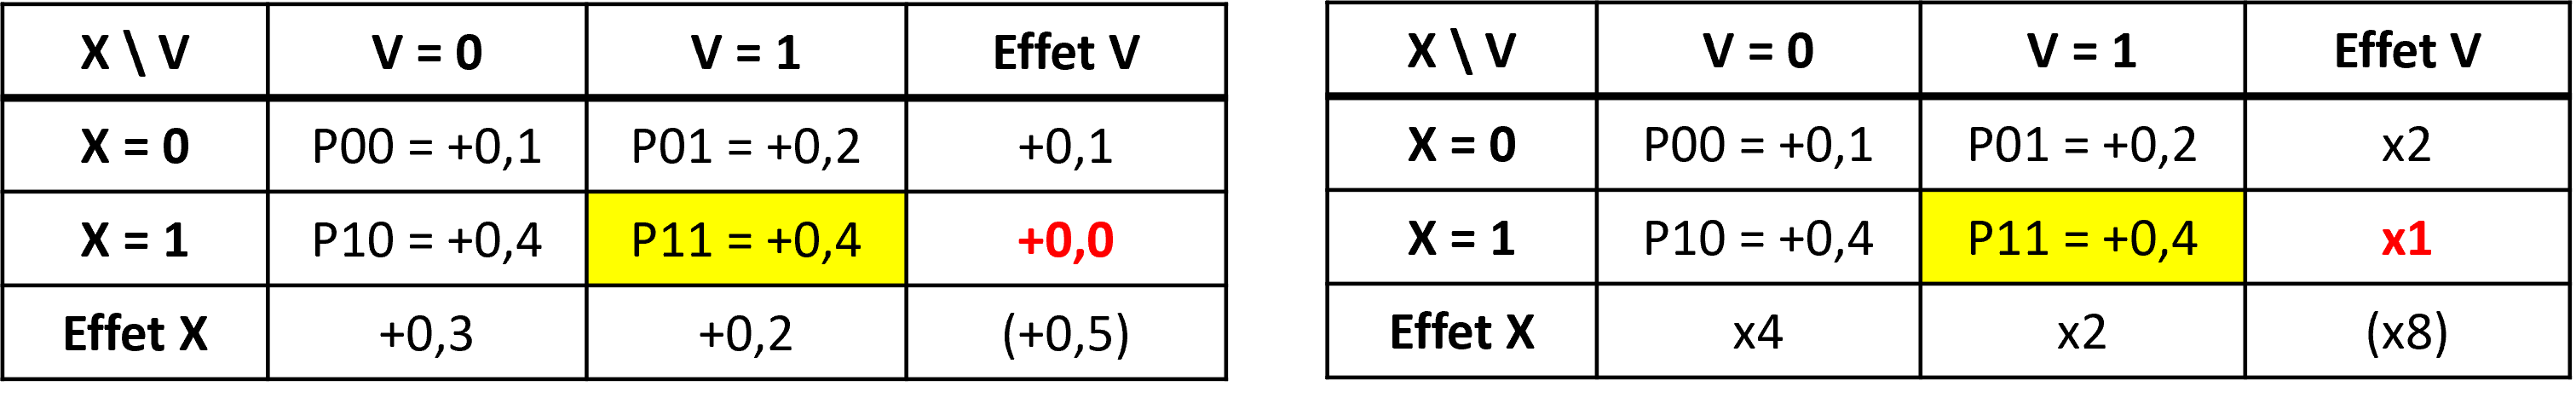
\includegraphics[width=0.9\textwidth,height=\textheight]{img/Image8.png}
\end{quote}

\begin{itemize}
\tightlist
\item
  \textbf{Interaction qualitative} de \(\small X\) en fonction de V, si l'effet de \(\small X\) dans une strate de \(\small V\) va dans la direction opposée de l'autre strate de \(\small V\).
\end{itemize}

\begin{quote}
Par exemple (ligne 7), \(\small V\) a un effet positif si \(\small X=0\) mais négatif si \(\small X=1\) :

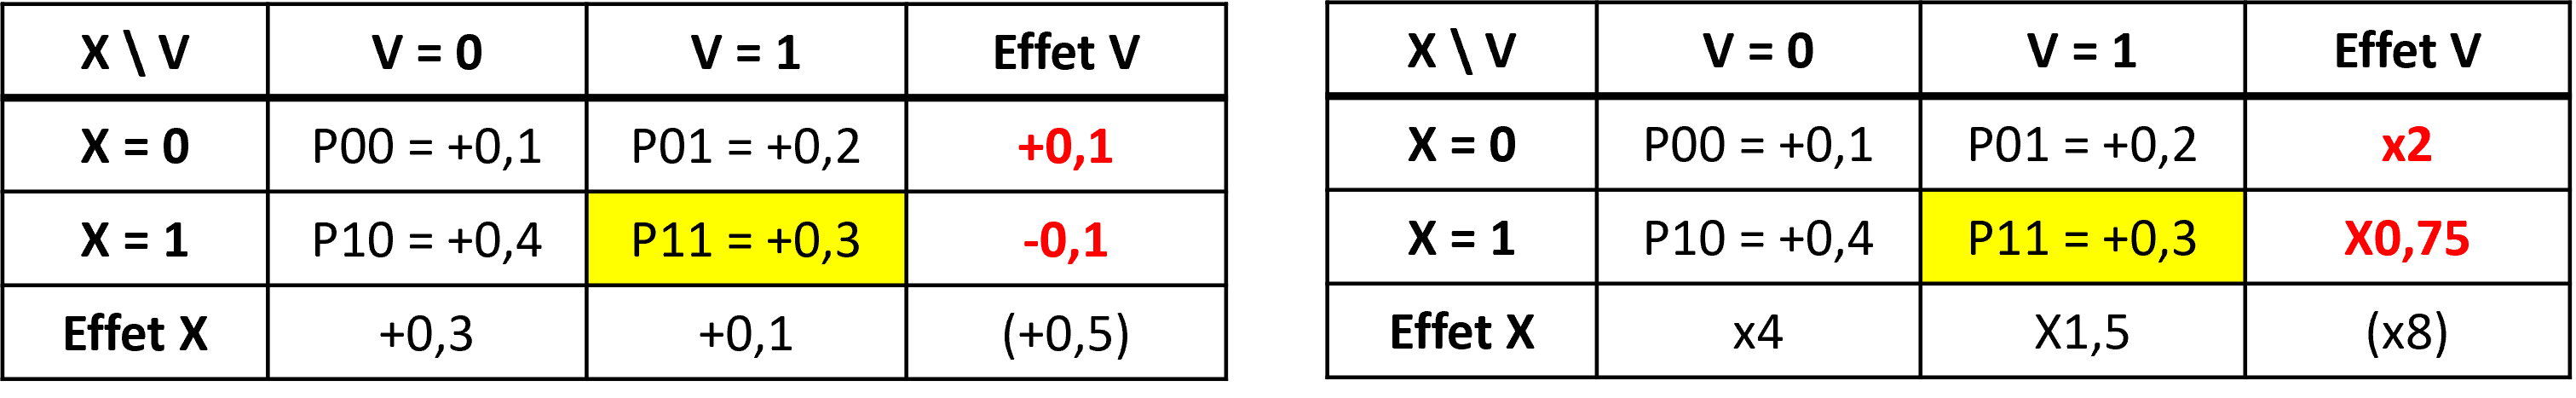
\includegraphics[width=0.9\textwidth,height=\textheight]{img/Image9.png}
\end{quote}

\begin{itemize}
\tightlist
\item
  \textbf{Antagonisme parfait} : l'effet joint est nul \(\small p_{11} - p_{00} = 0\), alors que les effets individuels sont positifs.
\end{itemize}

\begin{quote}
Par exemple (ligne 10), \(\small p_{11} - p_{00} = 0\) alors que \(\small p_{01} - p_{00} > 0\) et \(\small p_{10} - p_{00} > 0\)

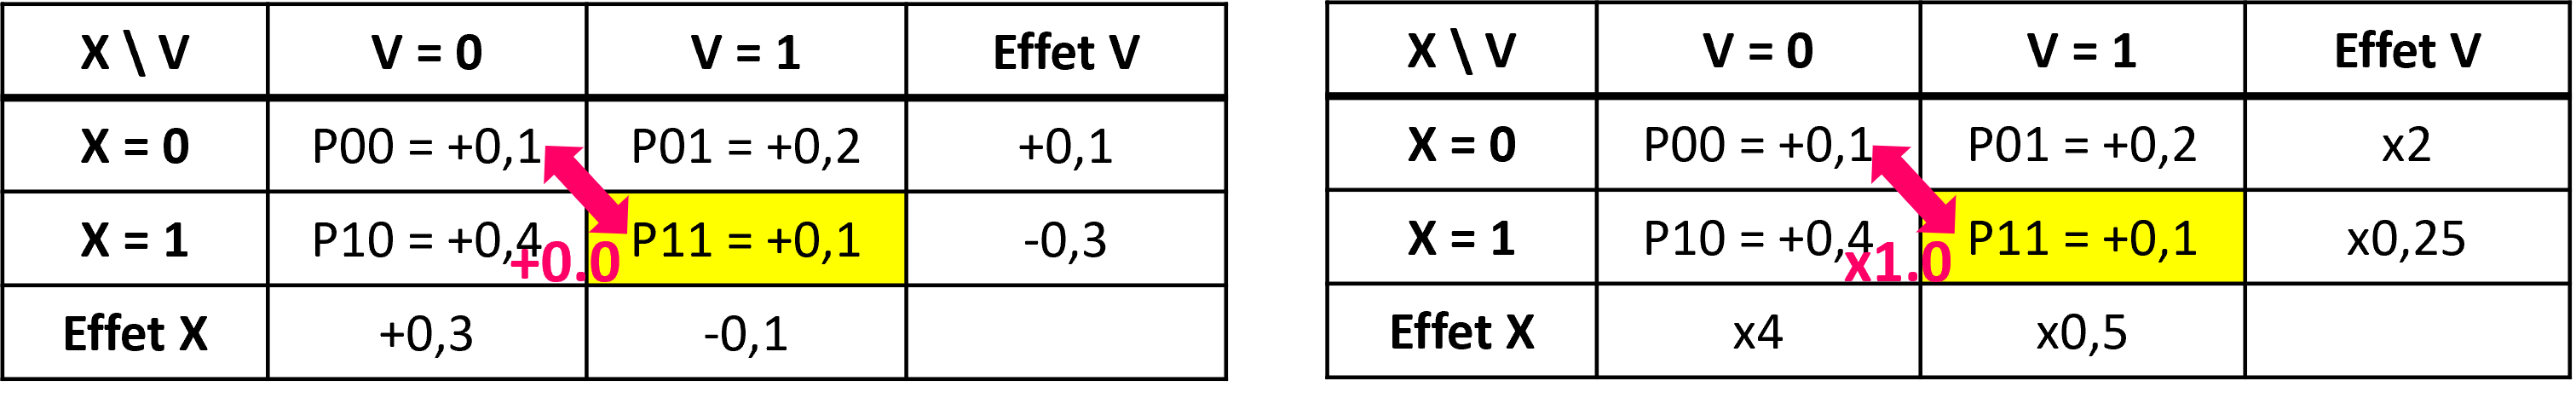
\includegraphics[width=0.9\textwidth,height=\textheight]{img/Image9b.png}
\end{quote}

\begin{itemize}
\tightlist
\item
  \textbf{Interaction inversée} (ligne 11): l'effet joint est négatif, alors que les effets individuels sont positifs.
\end{itemize}

\begin{quote}
Par exemple (ligne 10), \(\small p_{11} - p_{00} < 0\) alors que \(\small p_{01} - p_{00} > 0\) et \(\small p_{10} - p_{00} > 0\)

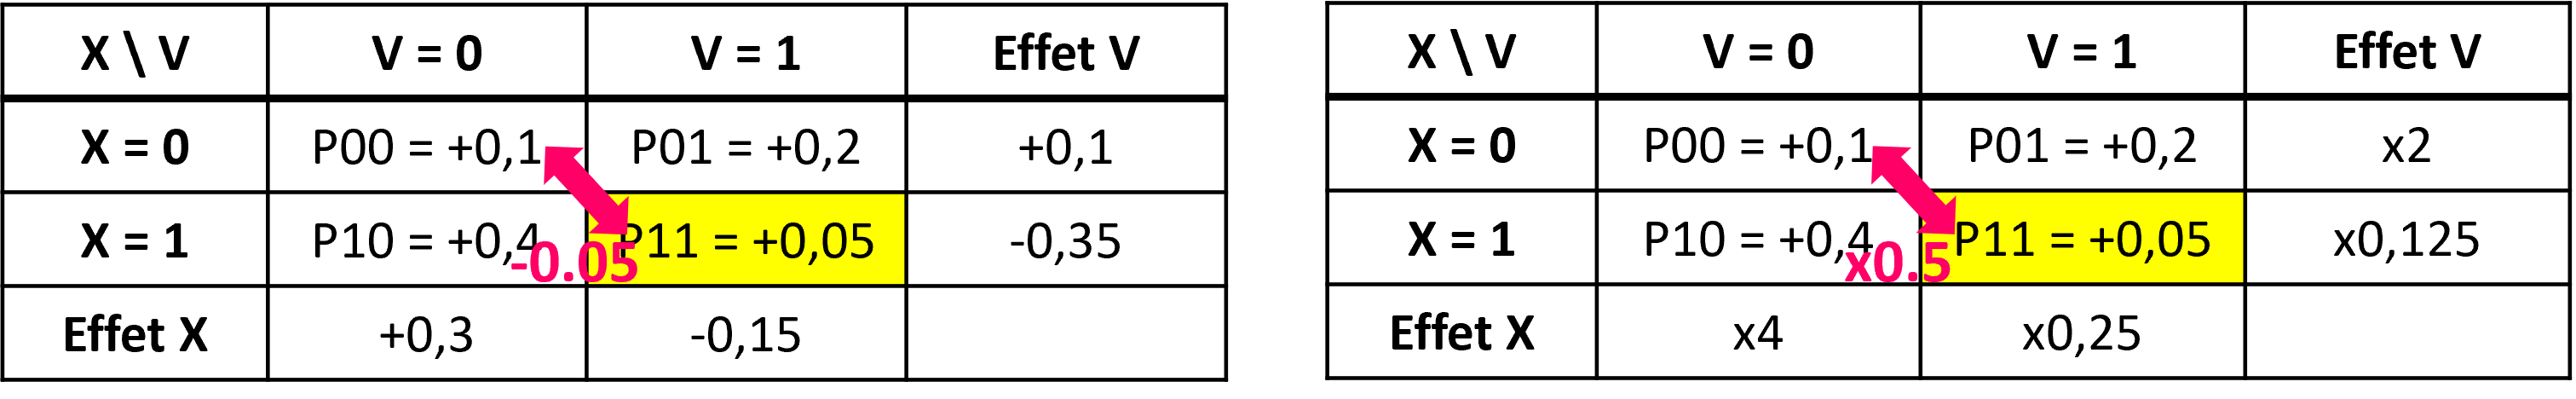
\includegraphics[width=0.9\textwidth,height=\textheight]{img/Image9c.png}
\end{quote}

\hypertarget{synthuxe8se-1}{%
\section{Synthèse}\label{synthuxe8se-1}}

Quelle échelle choisir pour mesurer un effet d'interaction ?

Même si en pratique l'échelle multiplicative est plus utilisée, car les outcomes sont souvent binaires en épidémiologie et donc les modèles logistiques sont souvent utilisés \citet{knol_recommendations_2012}, il semble y avoir un consensus pour privilégier plutôt l'échelle additive, plus appropriée pour évaluer l'utilité en santé publique \citet{vanderweele_tutorial_2014} \citet{knol_recommendations_2012}.

\begin{quote}
Si on reprend l'exemple ci dessous :

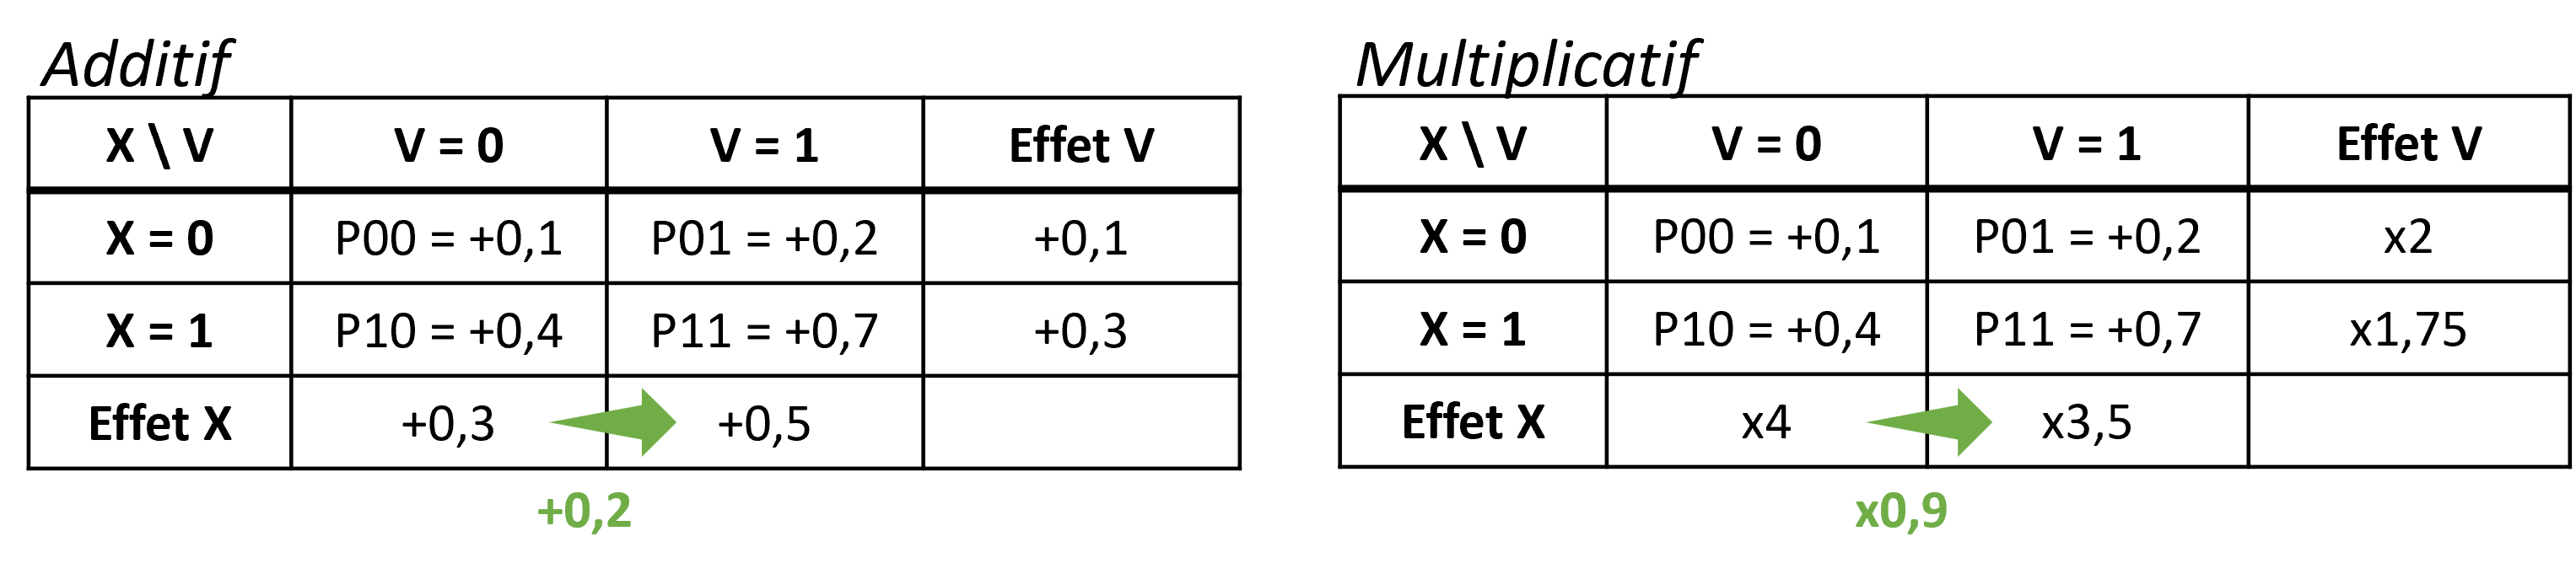
\includegraphics[width=0.9\textwidth,height=\textheight]{img/Image4b.png}

\(\small X\) représente un traitement dont on ne dispose que de 100 doses et \(\small Y\) un outcome de santé favorable (guérison).
Il faut choisir si on donne 100 doses au groupe \(\small V = 0\) ou au groupe \(\small V = 1\).

Si on donne 100 doses :

\begin{itemize}
\tightlist
\item
  au groupe \(\small V = 0\), 40 personnes seront guéries, soit 30 personnes de plus que l'évolution naturelle (40 - 10)
\item
  au groupe \(\small V = 1\), 70 personnes seront guéries, soit 50 personnes de plus que l'évolution naturelle (70 - 20).
\end{itemize}

Il semble donc préférable d'allouer les doses au groupe \(\small V=1\), car on guéri 20 personnes de plus (50 - 30).

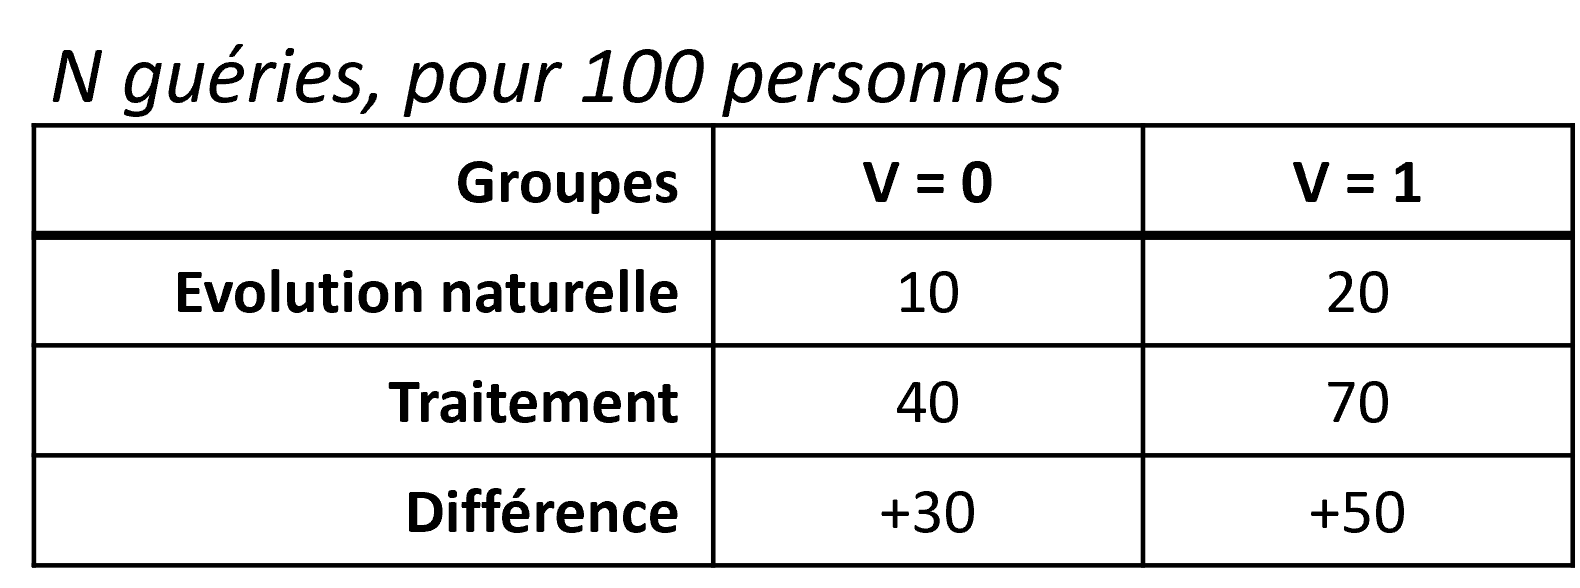
\includegraphics[width=0.4\textwidth,height=\textheight]{img/Image4c.png}

Pourtant si on avait réfléchi à partir de l'échelle multiplicative, on aurait choisi le groupe \(\small V=0\) car :

\begin{itemize}
\tightlist
\item
  l'effet du traitement est de RR=4 dans le groupe \(\small V = 0\) (\(\small \frac{40}{10} =4\)x plus de personnes guéries par rapport à l'évolution naturelle)
\item
  et de RR=3,5 dans le groupe \(\small V = 1\) (\(\small \frac{70}{20}) =3.5\)x plus de personnes guéries par rapport à l'évolution naturelle.
\end{itemize}

On peut donc conclure à un effet multiplicatif plus fort d'un traitement dans un groupe alors qu'en terme d'utilité (nombre de personnes favorablement impactées), l'échelle additive nous conduirait à choisir l'autre groupe\ldots{}
\end{quote}

Idéalement, les interactions devraient cependant être reportées sur les 2 échelles \citet{knol_recommendations_2012} \citet{vanderweele_tutorial_2014}.

\hypertarget{param}{%
\chapter{Types de paramètres}\label{param}}

Plusieurs paramètres peuvent être utilisés pour décrire une interaction, sur l'échelle additive ou multiplicative.

\hypertarget{avec-les-diffuxe9rences-de-risques-dr}{%
\section{Avec les différences de risques (DR)}\label{avec-les-diffuxe9rences-de-risques-dr}}

On a déjà défini un paramètre d'interaction sur l'échelle additive (AI) à partir des différences d'effets \citet{vanderweele_tutorial_2014} :

\begin{itemize}
\tightlist
\item
  \(\small AI = DR(X, V) - [DR(X|V=0) + DR(V|X=0)]\)
\item
  \(\small AI = (p_{11} - p_{00}) - [(p_{10} - p_{00}) + (p_{01} - p_{00})]\)
\item
  soit \(\small AI =p_{11} - p_{10} - p_{01} + p_{00}\)
\end{itemize}

\hypertarget{avec-les-risques-relatifs-rr}{%
\section{Avec les risques relatifs (RR)}\label{avec-les-risques-relatifs-rr}}

On a aussi défini un paramètre d'interaction sur l'échelle multiplicative (MI) à partir des risques relatifs \citet{vanderweele_tutorial_2014} :

\begin{itemize}
\tightlist
\item
  \(\small MI = \frac{RR_{11}}{RR_{10} \times RR_{01}}\)
\item
  soit \(\small MI = \frac{p_{11} / p_{00}}{(p_{10} / p_{00}) \times (p_{01} / p_{00})}\)
\item
  soit \(\small MI = \frac{p_{11} \times p_{00}}{p_{10} \times p_{01}}\)
\end{itemize}

\hypertarget{avec-les-odds-ratio-or}{%
\section{Avec les Odds Ratio (OR)}\label{avec-les-odds-ratio-or}}

Souvent en épidémiologie, lorsque l'outcome Y est binaire, les effets sont mesurés par des odds ratios estimés à partir de modèles de régression logistique.

Un paramètre d'interaction sur l'echelle multiplicative (\(\small MI_{OR}\)) peut être estimé à partir de ces OR \citet{vanderweele_tutorial_2014} :

\begin{itemize}
\tightlist
\item
  \(\small MI_{OR} = \frac{OR_{11}}{OR_{10} \times OR_{01}}\)
\end{itemize}

En général, la mesure \(\small MI_{OR}\) et \(\small MI_{RR}\) seront proches si l'outcome est rare \citet{vanderweele_tutorial_2014}.

\hypertarget{excuxe8s-de-risque-uxe0-partir-des-rr-reri}{%
\section{Excès de risque à partir des RR (RERI)}\label{excuxe8s-de-risque-uxe0-partir-des-rr-reri}}

Lorsque seulement les risques relatifs sont donnés mais que l'on souhaite évaluer l'interaction sur l'échelle additive, ``l'excès de risque du à l'interaction'' (RERI) ou ``interaction contrast ratio'' (ICR), peut être estimé à partir des risques relatifs \citet{vanderweele_tutorial_2014} :

\begin{align*}\small
RERI =& \frac{AI}{p_{00}} = \frac{p_{11} - p_{10} - p_{01} + p_{00}}{p_{00}}\\ 
\small RERI =& RR_{11} - RR_{10} - RR_{01} + 1
\end{align*}

On voit que le RERI correspond à l'interaction mesurée sur l'échelle additive, rapportée au risque de base \(p_{00}\).

Il faut noter que, bien que le RERI donne la direction (positive, négative ou nulle) de l'interaction additive, nous ne pouvons pas utiliser le RERI pour évaluer l'ampleur de l'interaction additive, à moins de connaître au moins \(\small p_{00}\).

Si l'on a seulement l'OR et que l'outcome est rare, les OR peuvent approximer les RR, on a donc :

\begin{itemize}
\tightlist
\item
  \(\small RERI_{OR} = OR_{11} - OR_{10} - OR_{01} + 1 \approx RERI_{RR}\)
\end{itemize}

\hypertarget{autres}{%
\section{Autres}\label{autres}}

D'autres paramètres ont aussi été proposés \citet{vanderweele_tutorial_2014}, tels que :

\hypertarget{le-synergie-index-si}{%
\subsection*{Le ``Synergie index'' (SI)}\label{le-synergie-index-si}}
\addcontentsline{toc}{subsection}{Le ``Synergie index'' (SI)}

Il s'agit d'un paramètre explorant l'interaction additive :

\begin{itemize}
\tightlist
\item
  \(\small S = \frac{RR_{11} - 1}{(RR_{10} - 1) + (RR_{01}-1)}\).
\end{itemize}

Il mesure l'augmentation relative du risque liée à l'exposition jointe, rapportée à la somme des augmentations relatives du risque liées à la 1ère et la 2ème exposition.

Pour rappel, l'augmentation relative du risque liée à l'exposition jointe correspond à l'augmentation absolue du risque (différence de risques), exprimée en pourcentage par rapport au risque de base \(p_{00}\).

\(\small ARR(X,V) = \frac{DR(X,V)}{p_{00}} = \frac{p_{11}-p_{00}}{p_{00}}= RR_{11}-1\)

L'augmentation relative du risque liée à l'exposition \(\small X\) ou \(\small V\), exprimées en pourcentage par rapport au risque de base \(p_{00}\) sont respectivement :

\begin{itemize}
\tightlist
\item
  \(\small ARR(X|V=0) = \frac{p_{10}-p_{00}}{p_{00}}= RR_{10}-1\)
\item
  et \(\small ARR(V|X=0) = \frac{p_{01}-p_{00}}{p_{00}}= RR_{01}-1\)
\end{itemize}

Une autre façon d'interpréter le ``Synergie index'' est d'indiquer que la différence liée à l'effet joint \(\small DR(X,V)\) est égale à \(S\) fois la somme des différences liées aux effets individuels \(\small DR(X|V=0) + DR(V|X=0)\) :

\(\small S = \frac{p_{11}-p_{00}}{(p_{10}-p_{00}) + (p_{01} - p_{00})}\)

Si le dénominateur est positif:

\begin{itemize}
\tightlist
\item
  si \(\small S > 1\), alors \(\small AI > 0\) et \(\small RERI_{RR} > 0\)
\item
  si \(\small S < 1\), alors \(\small AI < 0\) et \(\small RERI_{RR} < 0\)
\end{itemize}

L'interprétation de l'indice de synergie devient difficile dans les cas où l'effet de l'une des expositions a un effet négatif et que le dénominateur de \(S\) est inférieur à 1.

\hypertarget{proportion-attribuable-ap}{%
\subsection{Proportion attribuable (AP)}\label{proportion-attribuable-ap}}

Il s'agit aussi d'un paramètre explorant l'interaction additive :

\begin{itemize}
\tightlist
\item
  \(\small AP = \frac{RR_{11} - RR_{10} - RR_{01} + 1}{RR_{11}}\).
\end{itemize}

Ce paramètre mesure la proportion du risque dans le groupe doublement exposé qui est due à l'interaction.

L'AP est en lien avec le \(\small RERI_{RR}\) :

\begin{itemize}
\tightlist
\item
  AP \textgreater{} 0 si et seulement si \(\small RERI_{RR}\) \textgreater{} 0
\item
  AP \textless{} 0 si et seulement si \(\small RERI_{RR}\) \textless{} 0.
\end{itemize}

En fait \(\small AP = \frac{RERI_{RR}}{RR_{11}-1}\).

\hypertarget{part-estimations-interpruxe9tations-pruxe9sentations}{%
\part{Estimations, Interprétations, Présentations}\label{part-estimations-interpruxe9tations-pruxe9sentations}}

\hypertarget{pruxe9sentation-des-ruxe9sultats}{%
\chapter{Présentation des résultats}\label{pruxe9sentation-des-ruxe9sultats}}

\hypertarget{recommandations}{%
\section{Recommandations}\label{recommandations}}

Knol et VanderWeele ont émis des recommandations concernant la présentation des résultats d'une analyse d'interaction \citet{knol_recommendations_2012}. Ces recommandations sont :

\hypertarget{pour-une-analyse-dune-modification-deffet-de-small-x-sur-small-y-par-small-v}{%
\subsection*{\texorpdfstring{Pour une analyse d'une modification d'effet de \(\small X\) sur \(\small Y\) par \(\small V\)}{Pour une analyse d'une modification d'effet de \textbackslash small X sur \textbackslash small Y par \textbackslash small V}}\label{pour-une-analyse-dune-modification-deffet-de-small-x-sur-small-y-par-small-v}}
\addcontentsline{toc}{subsection}{Pour une analyse d'une modification d'effet de \(\small X\) sur \(\small Y\) par \(\small V\)}

\begin{itemize}
\tightlist
\item
  Présenter les effectifs dans chaque catégorie

  \begin{itemize}
  \tightlist
  \item
    avec et sans l'outcome (\(\small N_{x,v}(Y=1)\) et \(\small N_{x,v}(Y=0)\))
  \end{itemize}
\item
  Présenter les risques relatifs (RR), les OR ou les différences de risques (RD)

  \begin{itemize}
  \tightlist
  \item
    avec les intervalles de confiance (IC)
  \item
    pour chaque strate de \(\small X\) et de \(\small V\) avec une seule catégorie de référence
  \item
    (éventuellement prise comme la strate \(\small X \cap V\) présentant le plus faible risque de \(\small Y\)).
  \end{itemize}
\item
  Présenter les RR, OR ou RD avec les IC

  \begin{itemize}
  \tightlist
  \item
    de l'effet de \(\small X\) sur \(\small Y\) dans les strates de \(\small V\)
  \end{itemize}
\item
  Présenter les mesures de la modification de l'effet avec les IC, sur des échelles

  \begin{itemize}
  \tightlist
  \item
    additives (par exemple, RERI)
  \item
    et multiplicatives.
  \end{itemize}
\item
  Énumérer les facteurs de confusion pour lesquels la relation entre \(\small X\) et \(\small Y\) a été ajustée.
\end{itemize}

\hypertarget{interaction-small-xv-sur-small-y}{%
\subsection*{\texorpdfstring{Interaction \(\small X*V\) sur \(\small Y\)}{Interaction \textbackslash small X*V sur \textbackslash small Y}}\label{interaction-small-xv-sur-small-y}}
\addcontentsline{toc}{subsection}{Interaction \(\small X*V\) sur \(\small Y\)}

\begin{itemize}
\tightlist
\item
  Présenter les effectifs dans chaque catégorie

  \begin{itemize}
  \tightlist
  \item
    avec et sans l'outcome (\(\small N_{x,v}(Y=1)\) et \(\small N_{x,v}(Y=0)\))
  \end{itemize}
\item
  Présenter les risques relatifs (RR), les OR ou les différences de risques (RD)

  \begin{itemize}
  \tightlist
  \item
    avec les intervalles de confiance (IC)
  \item
    pour chaque strate de \(\small X\) et de \(\small V\) avec une seule catégorie de référence
  \item
    (éventuellement prise comme la strate \(\small X \cap V\) présentant le plus faible risque de \(\small Y\)).
  \end{itemize}
\item
  Présenter les RR, OR ou RD avec les IC

  \begin{itemize}
  \tightlist
  \item
    de l'effet de \(\small X\) sur \(\small Y\) dans les strates de \(\small V\)
  \item
    \textbf{et de \(\small V\) sur \(\small Y\) dans les strates de \(\small X\)}.
  \end{itemize}
\item
  Présenter les mesures de la modification de l'effet d'interaction avec les IC sur des échelles

  \begin{itemize}
  \tightlist
  \item
    additives (par exemple, RERI)
  \item
    et multiplicatives.
  \end{itemize}
\item
  Énumérer les facteurs de confusion pour lesquels la relation entre \(\small X\) et \(\small Y\) \textbf{et la relation entre \(\small V\) et \(\small Y\)} ont été ajustées.
\end{itemize}

\hypertarget{proposition}{%
\section{Proposition}\label{proposition}}

Ces recommandations sont très utiles lorsque les interactions ont été évaluées à partir de modèles de régression (logistiques, log-linéaires ou linéaires) permettant d'estimer directement des OR, des RR ou des DR, condionnellement aux facteurs de confusion.

En inférence causale, des assocations marginales plutôt que conditionnelles sont souvent estimées (que ce soit en termes de difference de risques, de risques relatifs ou d'odds ratio). Dans la suite de ce document, nous proposons une variante des recommandations de Knol et VanderWeele, adaptée à des estimations marginales. Nous proposons en effet :

\begin{itemize}
\tightlist
\item
  De présenter les effets marginaux ou proportions prédites de \(\small Y\) dans chaque strate \(\small X \cap V\),

  \begin{itemize}
  \tightlist
  \item
    plutôt les effectifs avec et sans l'outcome
  \end{itemize}
\item
  Ne pas forcément présenter une différence de risques ou un rapport de risques

  \begin{itemize}
  \tightlist
  \item
    pour chaque strate de \(\small X\) et de \(\small V\) avec une seule catégorie de référence
  \end{itemize}
\item
  Mais présenter les effets

  \begin{itemize}
  \tightlist
  \item
    de \(\small X\) dans chaque strate de \(\small V\)
  \item
    et de \(\small V\) dans chaque strate de \(\small X\) (si analyse d'interaction)
  \item
    sur une échelle multiplicative \textbf{et} additive.
  \end{itemize}
\end{itemize}

\hypertarget{simulations}{%
\chapter{Simulations}\label{simulations}}

Pour la description des différents types d'estimation, on a simulé des données selon le DAG suivant (toutes les variables sont binaires):

\begin{quote}
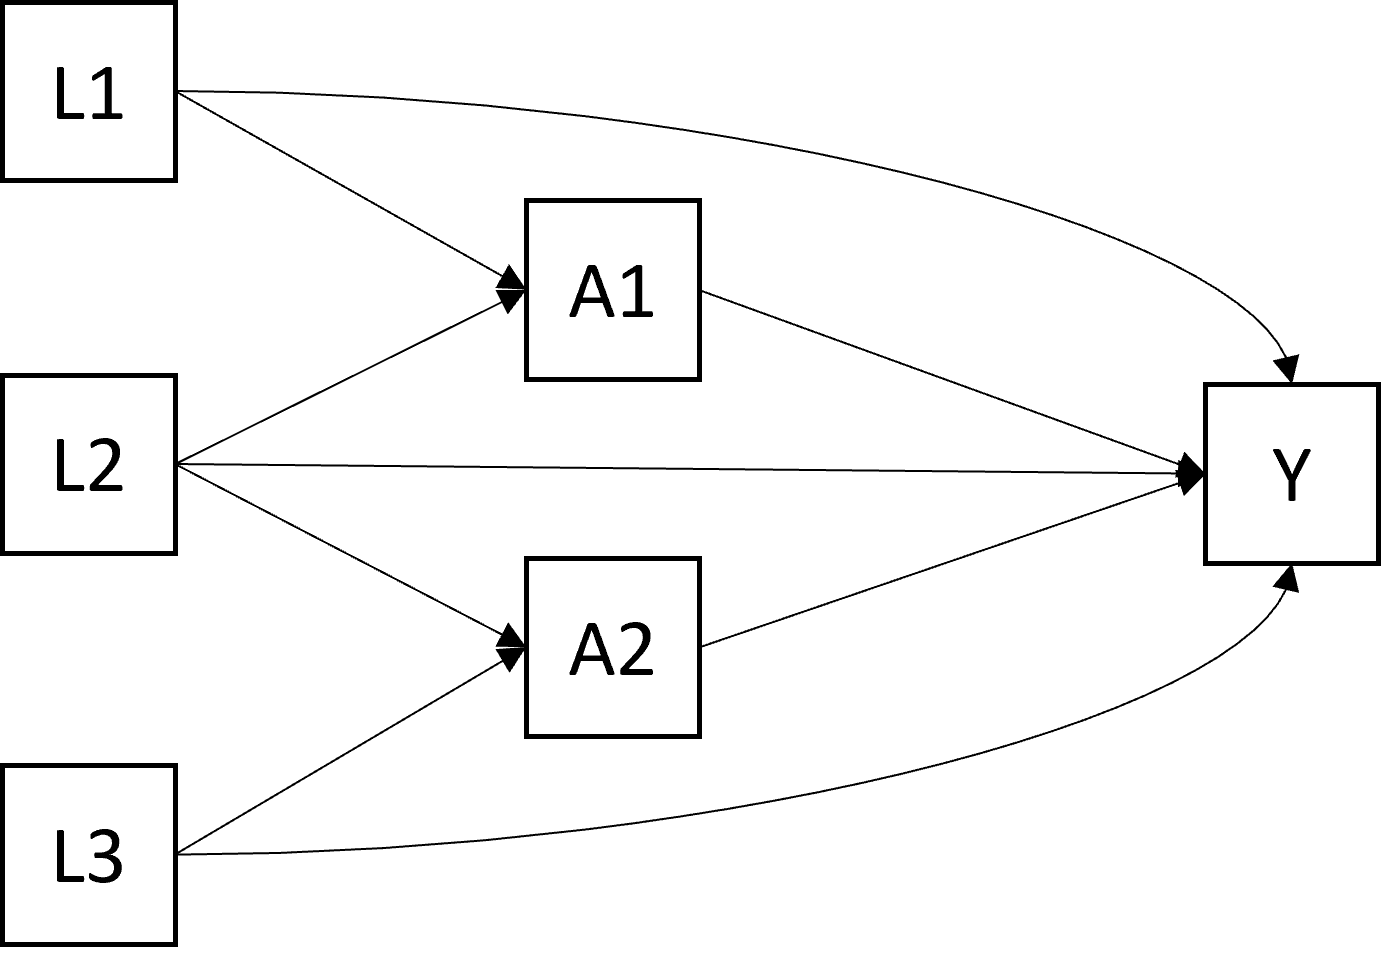
\includegraphics[width=0.5\textwidth,height=\textheight]{img/Image10.png}
\end{quote}

Les équations structurelles associées au DAG sont décrites ci-dessous, les paramètres correspondent aux paramètres renseignés dans le code de simulation.
\begin{align*}
\small P(L1 = 1) =& p_{L_1} \\
\small P(L2 = 1) =& p_{L_2} \\
\small P(L3 = 1) =& p_{L_3} \\
\small P(A1 = 1 \mid L1, L2) =& \beta_{A_1} + \beta_{L_1,A_1} L1 + \beta_{L_2,A_1} L2 \\
\small P(A2 = 1 \mid L1, L3) =& \beta_{A_2} + \beta_{L_1,A_2} L1 + \beta_{L_3,A_2} L3 \\
\small P(Y = 1 \mid L1, L2, L3, A1, A2) =& \beta_{Y} + \beta_{L_1,Y} L1 + \beta_{L_2,Y} L2 + \beta_{L_3,Y} L3 \\
                  & + \beta_{A_1,Y} A1 + \beta_{A_2,Y} A2 + \beta_{A_1 \ast A_2,Y} (A1 \ast A2)
\end{align*}

Le code ayant permis de simuler les données est le suivant :

\begin{Shaded}
\begin{Highlighting}[]
  \FunctionTok{rm}\NormalTok{(}\AttributeTok{list=}\FunctionTok{ls}\NormalTok{())}

\NormalTok{  param.causal.model }\OtherTok{\textless{}{-}} \ControlFlowTok{function}\NormalTok{(}\AttributeTok{p\_L1 =} \FloatTok{0.50}\NormalTok{, }\CommentTok{\# baseline confounders}
                                 \AttributeTok{p\_L2 =} \FloatTok{0.20}\NormalTok{, }\CommentTok{\# baseline confounders}
                                 \AttributeTok{p\_L3 =} \FloatTok{0.70}\NormalTok{, }\CommentTok{\# baseline confounders}
                                 \AttributeTok{b\_A1 =} \FloatTok{0.10}\NormalTok{,    }\CommentTok{\# modèle de A1}
                                 \AttributeTok{b\_L1\_A1 =} \FloatTok{0.15}\NormalTok{, }\CommentTok{\# modèle de A1}
                                 \AttributeTok{b\_L2\_A1 =} \FloatTok{0.25}\NormalTok{, }\CommentTok{\# modèle de A1}
                                 \AttributeTok{b\_A2 =} \FloatTok{0.15}\NormalTok{,    }\CommentTok{\# modèle de A2}
                                 \AttributeTok{b\_L1\_A2 =} \FloatTok{0.20}\NormalTok{, }\CommentTok{\# modèle de A2 }
                                 \AttributeTok{b\_L3\_A2 =} \FloatTok{0.20}\NormalTok{, }\CommentTok{\# modèle de A2}
                                 \AttributeTok{b\_Y =} \FloatTok{0.10}\NormalTok{,      }\CommentTok{\# modèle de Y}
                                 \AttributeTok{b\_L1\_Y =} \FloatTok{0.02}\NormalTok{,   }\CommentTok{\# modèle de Y}
                                 \AttributeTok{b\_L2\_Y =} \FloatTok{0.02}\NormalTok{,   }\CommentTok{\# modèle de Y}
                                 \AttributeTok{b\_L3\_Y =} \SpecialCharTok{{-}}\FloatTok{0.02}\NormalTok{,  }\CommentTok{\# modèle de Y}
                                 \AttributeTok{b\_A1\_Y =} \FloatTok{0.3}\NormalTok{,    }\CommentTok{\# modèle de Y}
                                 \AttributeTok{b\_A2\_Y =} \FloatTok{0.1}\NormalTok{,    }\CommentTok{\# modèle de Y}
                                 \AttributeTok{b\_A1A2\_Y =} \FloatTok{0.4}\NormalTok{ ) \{ }\CommentTok{\# \textless{}{-} effet d\textquotesingle{}interaction Delta)}

  \CommentTok{\# coefficients pour simuler l\textquotesingle{}exposition}
  \CommentTok{\# exposition A1  \# vérif}
  \FunctionTok{try}\NormalTok{(}\ControlFlowTok{if}\NormalTok{(b\_A1 }\SpecialCharTok{+}\NormalTok{ b\_L1\_A1 }\SpecialCharTok{+}\NormalTok{ b\_L1\_A1 }\SpecialCharTok{\textgreater{}} \DecValTok{1}\NormalTok{) }
    \FunctionTok{stop}\NormalTok{(}\StringTok{"la somme des coefficient du modèle A1 dépasse 100\%"}\NormalTok{))}
  
  \CommentTok{\# exposition A2  \# vérif}
  \FunctionTok{try}\NormalTok{(}\ControlFlowTok{if}\NormalTok{(b\_A2 }\SpecialCharTok{+}\NormalTok{ b\_L1\_A2 }\SpecialCharTok{+}\NormalTok{ b\_L3\_A2 }\SpecialCharTok{\textgreater{}} \DecValTok{1}\NormalTok{) }
    \FunctionTok{stop}\NormalTok{(}\StringTok{"la somme des coefficients du modèle A2 dépasse 100\%"}\NormalTok{))}
  
  \CommentTok{\# coefficients pour simuler l\textquotesingle{}outcome, vérif}
  \FunctionTok{try}\NormalTok{(}\ControlFlowTok{if}\NormalTok{(b\_Y }\SpecialCharTok{+}\NormalTok{ b\_L1\_Y }\SpecialCharTok{+}\NormalTok{ b\_L2\_Y }\SpecialCharTok{+}\NormalTok{ b\_L3\_Y }\SpecialCharTok{+}\NormalTok{ b\_A1\_Y }\SpecialCharTok{+}\NormalTok{ b\_A2\_Y }\SpecialCharTok{+}\NormalTok{ b\_A1A2\_Y }\SpecialCharTok{\textgreater{}} \DecValTok{1}\NormalTok{) }
    \FunctionTok{stop}\NormalTok{(}\StringTok{"la somme des coefficients du modèle Y dépasse 100\%"}\NormalTok{))}
  \FunctionTok{try}\NormalTok{(}\ControlFlowTok{if}\NormalTok{(b\_Y }\SpecialCharTok{+}\NormalTok{ b\_L1\_Y }\SpecialCharTok{+}\NormalTok{ b\_L2\_Y }\SpecialCharTok{+}\NormalTok{ b\_L3\_Y }\SpecialCharTok{+}\NormalTok{ b\_A1\_Y }\SpecialCharTok{+}\NormalTok{ b\_A2\_Y }\SpecialCharTok{+}\NormalTok{ b\_A1A2\_Y }\SpecialCharTok{\textless{}} \DecValTok{0}\NormalTok{) }
    \FunctionTok{stop}\NormalTok{(}\StringTok{"la somme des coefficients du modèle Y est inférieure à 0\%"}\NormalTok{))}
  
\NormalTok{  coef }\OtherTok{\textless{}{-}} \FunctionTok{list}\NormalTok{(}\FunctionTok{c}\NormalTok{(}\AttributeTok{p\_L1 =}\NormalTok{ p\_L1, }\AttributeTok{p\_L2 =}\NormalTok{ p\_L2, }\AttributeTok{p\_L3 =}\NormalTok{ p\_L3),}
               \FunctionTok{c}\NormalTok{(}\AttributeTok{b\_A1 =}\NormalTok{ b\_A1, }\AttributeTok{b\_L1\_A1 =}\NormalTok{ b\_L1\_A1, }\AttributeTok{b\_L2\_A1 =}\NormalTok{ b\_L2\_A1),}
               \FunctionTok{c}\NormalTok{(}\AttributeTok{b\_A2 =}\NormalTok{ b\_A2, }\AttributeTok{b\_L1\_A2 =}\NormalTok{ b\_L1\_A2, }\AttributeTok{b\_L3\_A2 =}\NormalTok{ b\_L3\_A2),}
               \FunctionTok{c}\NormalTok{(}\AttributeTok{b\_Y =}\NormalTok{ b\_Y, }\AttributeTok{b\_L1\_Y =}\NormalTok{ b\_L1\_Y, }\AttributeTok{b\_L2\_Y =}\NormalTok{ b\_L2\_Y, }\AttributeTok{b\_L3\_Y =}\NormalTok{ b\_L3\_Y,}
                 \AttributeTok{b\_A1\_Y =}\NormalTok{ b\_A1\_Y, }\AttributeTok{b\_A2\_Y =}\NormalTok{ b\_A2\_Y, }\AttributeTok{b\_A1A2\_Y =}\NormalTok{ b\_A1A2\_Y))}
  \FunctionTok{return}\NormalTok{(coef)}
\NormalTok{\}}

\NormalTok{generate.data }\OtherTok{\textless{}{-}} \ControlFlowTok{function}\NormalTok{(N, }\AttributeTok{b =}  \FunctionTok{param.causal.model}\NormalTok{()) \{}
  
\NormalTok{  L1 }\OtherTok{\textless{}{-}} \FunctionTok{rbinom}\NormalTok{(N, }\AttributeTok{size =} \DecValTok{1}\NormalTok{, }\AttributeTok{prob =}\NormalTok{ b[[}\DecValTok{1}\NormalTok{]][}\StringTok{"p\_L1"}\NormalTok{]) }
\NormalTok{  L2 }\OtherTok{\textless{}{-}} \FunctionTok{rbinom}\NormalTok{(N, }\AttributeTok{size =} \DecValTok{1}\NormalTok{, }\AttributeTok{prob =}\NormalTok{ b[[}\DecValTok{1}\NormalTok{]][}\StringTok{"p\_L2"}\NormalTok{])}
\NormalTok{  L3 }\OtherTok{\textless{}{-}} \FunctionTok{rbinom}\NormalTok{(N, }\AttributeTok{size =} \DecValTok{1}\NormalTok{, }\AttributeTok{prob =}\NormalTok{ b[[}\DecValTok{1}\NormalTok{]][}\StringTok{"p\_L3"}\NormalTok{])}
\NormalTok{  A1 }\OtherTok{\textless{}{-}} \FunctionTok{rbinom}\NormalTok{(N, }\AttributeTok{size =} \DecValTok{1}\NormalTok{, }\AttributeTok{prob =}\NormalTok{ b[[}\DecValTok{2}\NormalTok{]][}\StringTok{"b\_A1"}\NormalTok{] }\SpecialCharTok{+} 
\NormalTok{                 (b[[}\DecValTok{2}\NormalTok{]][}\StringTok{"b\_L1\_A1"}\NormalTok{] }\SpecialCharTok{*}\NormalTok{ L1) }\SpecialCharTok{+}\NormalTok{ (b[[}\DecValTok{2}\NormalTok{]][}\StringTok{"b\_L2\_A1"}\NormalTok{] }\SpecialCharTok{*}\NormalTok{ L2))}
\NormalTok{  A2 }\OtherTok{\textless{}{-}} \FunctionTok{rbinom}\NormalTok{(N, }\AttributeTok{size =} \DecValTok{1}\NormalTok{, }\AttributeTok{prob =}\NormalTok{ b[[}\DecValTok{3}\NormalTok{]][}\StringTok{"b\_A2"}\NormalTok{] }\SpecialCharTok{+} 
\NormalTok{                 (b[[}\DecValTok{3}\NormalTok{]][}\StringTok{"b\_L1\_A2"}\NormalTok{] }\SpecialCharTok{*}\NormalTok{ L1) }\SpecialCharTok{+}\NormalTok{ (b[[}\DecValTok{3}\NormalTok{]][}\StringTok{"b\_L3\_A2"}\NormalTok{] }\SpecialCharTok{*}\NormalTok{ L3))}
\NormalTok{  Y }\OtherTok{\textless{}{-}} \FunctionTok{rbinom}\NormalTok{(N, }\AttributeTok{size =} \DecValTok{1}\NormalTok{, }\AttributeTok{prob =}\NormalTok{ (b[[}\DecValTok{4}\NormalTok{]][}\StringTok{"b\_Y"}\NormalTok{] }\SpecialCharTok{+} 
\NormalTok{                                     (b[[}\DecValTok{4}\NormalTok{]][}\StringTok{"b\_L1\_Y"}\NormalTok{] }\SpecialCharTok{*}\NormalTok{ L1) }\SpecialCharTok{+} 
\NormalTok{                                     (b[[}\DecValTok{4}\NormalTok{]][}\StringTok{"b\_L2\_Y"}\NormalTok{] }\SpecialCharTok{*}\NormalTok{ L2) }\SpecialCharTok{+}
\NormalTok{                                     (b[[}\DecValTok{4}\NormalTok{]][}\StringTok{"b\_L3\_Y"}\NormalTok{] }\SpecialCharTok{*}\NormalTok{ L3) }\SpecialCharTok{+}  
\NormalTok{                                     (b[[}\DecValTok{4}\NormalTok{]][}\StringTok{"b\_A1\_Y"}\NormalTok{] }\SpecialCharTok{*}\NormalTok{ A1) }\SpecialCharTok{+} 
\NormalTok{                                     (b[[}\DecValTok{4}\NormalTok{]][}\StringTok{"b\_A2\_Y"}\NormalTok{] }\SpecialCharTok{*}\NormalTok{ A2) }\SpecialCharTok{+} 
\NormalTok{                                     (b[[}\DecValTok{4}\NormalTok{]][}\StringTok{"b\_A1A2\_Y"}\NormalTok{] }\SpecialCharTok{*}\NormalTok{ A1 }\SpecialCharTok{*}\NormalTok{ A2)) )}
\NormalTok{  data.sim }\OtherTok{\textless{}{-}} \FunctionTok{data.frame}\NormalTok{(L1, L2, L3, A1, A2, Y)}
  \FunctionTok{return}\NormalTok{(data.sim)}
\NormalTok{\}}

\DocumentationTok{\#\#\#\# On simule une base de données}
  \FunctionTok{set.seed}\NormalTok{(}\DecValTok{12345}\NormalTok{)}
  \CommentTok{\# b =  param.causal.model(b\_A1A2\_Y = {-}0.45)}
\NormalTok{  b }\OtherTok{=} \FunctionTok{param.causal.model}\NormalTok{()}
\NormalTok{  df }\OtherTok{\textless{}{-}} \FunctionTok{generate.data}\NormalTok{(}\AttributeTok{N =} \DecValTok{10000}\NormalTok{, }\AttributeTok{b =}\NormalTok{ b)}
  \FunctionTok{summary}\NormalTok{(df)}
  \FunctionTok{prop.table}\NormalTok{(}\FunctionTok{table}\NormalTok{(df}\SpecialCharTok{$}\NormalTok{Y, df}\SpecialCharTok{$}\NormalTok{A1, df}\SpecialCharTok{$}\NormalTok{A2, }\AttributeTok{deparse.level =} \DecValTok{2}\NormalTok{))}
\end{Highlighting}
\end{Shaded}

Au final, les probabilités de l'outcome P(Y=1), dans chaque catégorie sont :

\begin{table}
\centering
\begin{tabular}{lrlr}
\toprule
A2 & label & levels & value\\
\midrule
0 & A1 & 0 & 0.10 (0.30)\\
0 &  & 1 & 0.41 (0.49)\\
1 & A1 & 0 & 0.20 (0.40)\\
1 &  & 1 & 0.90 (0.30)\\
\bottomrule
\end{tabular}
\end{table}

Les paramètres utilisés pour simuler les données ont été choisis de sorte que les ``vraies'' valeurs des paramètres de la distribution correspondent au tableau présenté au paragraphe \ref{echelle} ``Mesure des interactions''.

\hypertarget{regression}{%
\chapter{A partir de modèles de régression}\label{regression}}

Dans une première étape exploratoire, on peut simplement utiliser les modèles de régression habituels : les modèles de régression logistique et linéaire.

\hypertarget{ruxe9gression-logistique}{%
\section{Régression logistique}\label{ruxe9gression-logistique}}

Lorsque l'on étudie un outcome binaire, on utilise souvent les modèles de régression logistique.

\begin{verbatim}
## 
## Call:
## glm(formula = Y ~ as.factor(A1) + as.factor(A2) + as.factor(A1) * 
##     as.factor(A2) + as.factor(L1) + as.factor(L2) + as.factor(L3), 
##     family = binomial, data = df_f)
## 
## Coefficients:
##                               Estimate Std. Error z value Pr(>|z|)    
## (Intercept)                   -2.16540    0.06708 -32.281  < 2e-16 ***
## as.factor(A1)1                 1.75607    0.07604  23.093  < 2e-16 ***
## as.factor(A2)1                 0.75332    0.06831  11.028  < 2e-16 ***
## as.factor(L1)1                 0.15753    0.05702   2.763  0.00573 ** 
## as.factor(L2)1                 0.14128    0.06878   2.054  0.03996 *  
## as.factor(L3)1                -0.14926    0.06141  -2.431  0.01507 *  
## as.factor(A1)1:as.factor(A2)1  1.78587    0.14131  12.638  < 2e-16 ***
## ---
## Signif. codes:  0 '***' 0.001 '**' 0.01 '*' 0.05 '.' 0.1 ' ' 1
## 
## (Dispersion parameter for binomial family taken to be 1)
## 
##     Null deviance: 11037.7  on 9999  degrees of freedom
## Residual deviance:  8460.4  on 9993  degrees of freedom
## AIC: 8474.4
## 
## Number of Fisher Scoring iterations: 4
\end{verbatim}

A partir de cette sortie, on peut extraire :

\begin{itemize}
\tightlist
\item
  \textbf{A1\textbar A2=0}

  \begin{itemize}
  \tightlist
  \item
    à partir du coefficient \texttt{as.factor(A1)1}
  \item
    qui correspond à l'effet de A1 dans la catégorie de référence de A2,
  \item
    soit \(\small OR_{A1|A2=0} = exp(1.756) =\) 5.789.
  \end{itemize}
\item
  \textbf{A1\textbar A2=1}

  \begin{itemize}
  \tightlist
  \item
    à partir du coefficient \texttt{as.factor(A1)1:as.factor(A2)1},
  \item
    qui correspond à la différence d'effet de A1 quand on passe dans l'autre catégorie de A2.
  \item
    L'effet de A1 dans la catégorie A2=1 est donc
  \item
    \(\small OR_{A1|A2=1} = exp(1.756+1.786) =\) 34.536.
  \end{itemize}
\item
  \textbf{L'interaction multiplicative (IM)}

  \begin{itemize}
  \tightlist
  \item
    peut être estimée à partir du coefficient \texttt{as.factor(A1)1:as.factor(A2)1}
  \item
    par \(\small IM = exp(1.786) =\) 5.966,
  \item
    qu'on peut retrouver en faisant \(\small OR_{A1|A2=1}/ OR_{A1|A2=0}\).
  \item
    Ici l'interaction est significative (p-value \textgreater0.05).
  \end{itemize}
\item
  \textbf{A2\textbar A1=0} et \textbf{A2\textbar A1=1}

  \begin{itemize}
  \tightlist
  \item
    On aurait aussi pu décrire l'interaction à partir de l'effet d'A2 dans chaque strate de A1
  \item
    à partir de \texttt{as.factor(A2)1} et \texttt{as.factor(A1)1:as.factor(A2)1},
  \item
    avec : \(\small OR_{A2|A1=0} = exp(0.753) =\) 2.123
  \item
    et \(\small OR_{A2|A1=1} = exp(0.753+1.786) =\) 12.667
  \end{itemize}
\item
  \textbf{L'interaction additive}

  \begin{itemize}
  \tightlist
  \item
    On peut explorer l'interaction sur l'échelle additive en estimant le RERI par
  \item
    \(\small RERI \approx OR_{11} - OR_{10} - OR_{01} + 1 =\)
  \item
    \(\small OR_{A1,A2} - OR_{A1|A2=0} - OR_{A2|A1=0} + 1 =\)
  \item
    \(\small exp(1.786+0.753+1.786) - exp(1.786) - exp(0.753) + 1 =\) 68.477.
  \end{itemize}
\end{itemize}

En résumé, (le package \texttt{finalfit} permet de sortir quelques résultats proprement) :

\begin{Shaded}
\begin{Highlighting}[]
\NormalTok{explanatory }\OtherTok{=} \FunctionTok{c}\NormalTok{(}\StringTok{"as.factor(A1)"}\NormalTok{,}
                \StringTok{"as.factor(A2)"}\NormalTok{,}
                \StringTok{"as.factor(A1)*as.factor(A2)"}\NormalTok{, }
                \StringTok{"as.factor(L1)"}\NormalTok{,}
                \StringTok{"as.factor(L2)"}\NormalTok{, }
                \StringTok{"as.factor(L3)"}\NormalTok{)}
\NormalTok{dependent }\OtherTok{=} \StringTok{"Y"}

\NormalTok{df\_f }\SpecialCharTok{\%\textgreater{}\%}
  \FunctionTok{finalfit}\NormalTok{(dependent, explanatory)}\OtherTok{{-}\textgreater{}}\NormalTok{ t}

\CommentTok{\# le tableau t entier peut être imprimé, mais ici je sélectionne seulement les effets d\textquotesingle{}intéret }
\CommentTok{\# pour éviter la table 2 fallacy (les coefficient des facteurs de confusion L ne sont pas interprétables)}

\FunctionTok{cbind}\NormalTok{(}\AttributeTok{names =} \FunctionTok{c}\NormalTok{(}\StringTok{"A1|A2=0"}\NormalTok{, }\StringTok{"A2|A1=0"}\NormalTok{, }\StringTok{"Interaction"}\NormalTok{), }
      \AttributeTok{OR =}\NormalTok{ t[}\FunctionTok{c}\NormalTok{(}\DecValTok{12}\NormalTok{,}\DecValTok{14}\NormalTok{,}\DecValTok{13}\NormalTok{),}\DecValTok{6}\NormalTok{]) }\SpecialCharTok{\%\textgreater{}\%}
\NormalTok{  as.data.frame }\SpecialCharTok{\%\textgreater{}\%} 
      \FunctionTok{kbl}\NormalTok{() }\SpecialCharTok{\%\textgreater{}\%}
      \FunctionTok{kable\_classic}\NormalTok{() }
\end{Highlighting}
\end{Shaded}

\begin{table}
\centering
\begin{tabular}[t]{l|l}
\hline
names & OR\\
\hline
A1|A2=0 & 5.79 (4.99-6.72, p<0.001)\\
\hline
A2|A1=0 & 2.12 (1.86-2.43, p<0.001)\\
\hline
Interaction & 5.96 (4.54-7.90, p<0.001)\\
\hline
\end{tabular}
\end{table}

Attention, les modèles de régressions logistiques sont ici biaisés car les données sont générées à partir de modèles additifs.

\hypertarget{ruxe9gression-lineaire}{%
\section{Régression lineaire}\label{ruxe9gression-lineaire}}

Même si l'outcome binaire, on peut en théorie utiliser un modèle de régression linéaire et explorer les effets sur une échelle additive. Si l'outcome est quantitatif, on utilise aussi, en général, les modèles de régression linéaire.

\begin{verbatim}
## 
## Call:
## lm(formula = Y ~ as.factor(A1) + as.factor(A2) + as.factor(A1) * 
##     as.factor(A2) + as.factor(L1) + as.factor(L2) + as.factor(L3), 
##     data = df)
## 
## Residuals:
##      Min       1Q   Median       3Q      Max 
## -0.93110 -0.19602 -0.10494 -0.08426  0.91574 
## 
## Coefficients:
##                                Estimate Std. Error t value Pr(>|t|)    
## (Intercept)                    0.103835   0.008146  12.746  < 2e-16 ***
## as.factor(A1)1                 0.300796   0.011592  25.948  < 2e-16 ***
## as.factor(A2)1                 0.092280   0.008671  10.642  < 2e-16 ***
## as.factor(L1)1                 0.020677   0.007495   2.759  0.00581 ** 
## as.factor(L2)1                 0.019476   0.009410   2.070  0.03851 *  
## as.factor(L3)1                -0.019574   0.008085  -2.421  0.01549 *  
## as.factor(A1)1:as.factor(A2)1  0.394034   0.017854  22.070  < 2e-16 ***
## ---
## Signif. codes:  0 '***' 0.001 '**' 0.01 '*' 0.05 '.' 0.1 ' ' 1
## 
## Residual standard error: 0.3615 on 9993 degrees of freedom
## Multiple R-squared:  0.2856, Adjusted R-squared:  0.2852 
## F-statistic: 665.8 on 6 and 9993 DF,  p-value: < 2.2e-16
\end{verbatim}

A partir de cette sortie, on peut extraire :

\begin{itemize}
\tightlist
\item
  \textbf{A1\textbar A2=0}

  \begin{itemize}
  \tightlist
  \item
    à partir du coefficient \texttt{as.factor(A1)1}
  \item
    qui correspond à l'effet de A1 dans la catégorie de référence de A2,
  \item
    soit \(\small DR = +30,08 \%\).
  \end{itemize}
\item
  \textbf{A1\textbar A2=1}

  \begin{itemize}
  \tightlist
  \item
    à partir du coefficient \texttt{as.factor(A1)1:as.factor(A2)1},
  \item
    qui correspond à la différence d'effet de A1 quand on passe dans l'autre catégorie de A2.
  \item
    L'effet de A1 dans la catégorie A2=1 est donc
  \item
    \(\small DR = 30.08+39.40 =\) 69.48 \%.
  \end{itemize}
\item
  \textbf{L'interaction additive}

  \begin{itemize}
  \tightlist
  \item
    à partir du coefficient \texttt{as.factor(A1)1:as.factor(A2)1}
  \item
    avec \(\small AI = +39.40 \%\),
  \item
    qu'on peut retrouver en faisant \(\small DR(A1|A2=1) - DR(A1|A2=0)\).
  \item
    Ici l'interaction est significative (p-value \textgreater0.05).
  \end{itemize}
\item
  \textbf{A2\textbar A1=0} et \textbf{A2\textbar A1=1}

  \begin{itemize}
  \tightlist
  \item
    On aurait aussi pu décrire cette interaction à partir de l'effet d'A2 dans chaque strate de A1
  \item
    à partir de \texttt{as.factor(A2)1} et \texttt{as.factor(A1)1:as.factor(A2)1},
  \item
    avec : \(\small DR_{A1|A2=0} = +9.23\%\)
  \item
    et \(\small DR_{A1|A2=1} = 9.23+39.40 =\) 48.63\%.
  \end{itemize}
\end{itemize}

En résumé, (le package \texttt{finalfit} permet de sortir quelques résultats proprement) :

\begin{Shaded}
\begin{Highlighting}[]
\NormalTok{explanatory }\OtherTok{=} \FunctionTok{c}\NormalTok{(}\StringTok{"as.factor(A1)"}\NormalTok{,}
                \StringTok{"as.factor(A2)"}\NormalTok{,}
                \StringTok{"as.factor(A1)*as.factor(A2)"}\NormalTok{, }
                \StringTok{"as.factor(L1)"}\NormalTok{,}
                \StringTok{"as.factor(L2)"}\NormalTok{, }
                \StringTok{"as.factor(L3)"}\NormalTok{)}
\NormalTok{dependent }\OtherTok{=} \StringTok{"Y"}
\NormalTok{df }\SpecialCharTok{\%\textgreater{}\%}
  \FunctionTok{finalfit}\NormalTok{(dependent, explanatory)}\OtherTok{{-}\textgreater{}}\NormalTok{ t}

\FunctionTok{cbind}\NormalTok{(}\AttributeTok{names =} \FunctionTok{c}\NormalTok{(}\StringTok{"A1|A2=0"}\NormalTok{, }\StringTok{"A2|A1=0"}\NormalTok{, }\StringTok{"Interaction"}\NormalTok{), }\AttributeTok{DR =}\NormalTok{ t[}\FunctionTok{c}\NormalTok{(}\DecValTok{12}\NormalTok{,}\DecValTok{14}\NormalTok{,}\DecValTok{13}\NormalTok{),}\DecValTok{6}\NormalTok{]) }\SpecialCharTok{\%\textgreater{}\%}
\NormalTok{  as.data.frame }\SpecialCharTok{\%\textgreater{}\%} 
      \FunctionTok{kbl}\NormalTok{() }\SpecialCharTok{\%\textgreater{}\%}
      \FunctionTok{kable\_classic}\NormalTok{() }
\end{Highlighting}
\end{Shaded}

\begin{table}
\centering
\begin{tabular}[t]{l|l}
\hline
names & DR\\
\hline
A1|A2=0 & 0.30 (0.28 to 0.32, p<0.001)\\
\hline
A2|A1=0 & 0.09 (0.08 to 0.11, p<0.001)\\
\hline
Interaction & 0.39 (0.36 to 0.43, p<0.001)\\
\hline
\end{tabular}
\end{table}

\hypertarget{conf}{%
\chapter{Analyses confirmatoires}\label{conf}}

\hypertarget{estimation-par-g-computation}{%
\section{Estimation par G-computation}\label{estimation-par-g-computation}}

Il s'agit d'une ``G-method'' qui peut être décrite comme une ``standardisation'' par régression (Hernàn \citet{hernan2020causal}). Le principe est le suivant :

\begin{Shaded}
\begin{Highlighting}[]
\DocumentationTok{\#\# 1.a) on crée 4 tables correspondant aux 4 interventions contrefactuelles}
\NormalTok{    df.A1\_0.A2\_0 }\OtherTok{\textless{}{-}}\NormalTok{ df.A1\_1.A2\_0 }\OtherTok{\textless{}{-}}\NormalTok{ df.A1\_0.A2\_1 }\OtherTok{\textless{}{-}}\NormalTok{ df.A1\_1.A2\_1 }\OtherTok{\textless{}{-}}\NormalTok{ df}

    \CommentTok{\# scénario do(A1 = 0, A2 = 0) pour toute la population}
\NormalTok{    df.A1\_0.A2\_0}\SpecialCharTok{$}\NormalTok{A1 }\OtherTok{\textless{}{-}}\NormalTok{ df.A1\_0.A2\_0}\SpecialCharTok{$}\NormalTok{A2 }\OtherTok{\textless{}{-}} \FunctionTok{rep}\NormalTok{(}\DecValTok{0}\NormalTok{, }\FunctionTok{nrow}\NormalTok{(df))}
    
    \CommentTok{\# scénario do(A1 = 1, A2 = 0) pour toute la population}
\NormalTok{    df.A1\_1.A2\_0}\SpecialCharTok{$}\NormalTok{A1 }\OtherTok{\textless{}{-}} \FunctionTok{rep}\NormalTok{(}\DecValTok{1}\NormalTok{, }\FunctionTok{nrow}\NormalTok{(df))}
\NormalTok{    df.A1\_1.A2\_0}\SpecialCharTok{$}\NormalTok{A2 }\OtherTok{\textless{}{-}} \FunctionTok{rep}\NormalTok{(}\DecValTok{0}\NormalTok{, }\FunctionTok{nrow}\NormalTok{(df))}
    
    \CommentTok{\# scénario do(A1 = 0, A2 = 1) pour toute la population}
\NormalTok{    df.A1\_0.A2\_1}\SpecialCharTok{$}\NormalTok{A1 }\OtherTok{\textless{}{-}} \FunctionTok{rep}\NormalTok{(}\DecValTok{0}\NormalTok{, }\FunctionTok{nrow}\NormalTok{(df))}
\NormalTok{    df.A1\_0.A2\_1}\SpecialCharTok{$}\NormalTok{A2 }\OtherTok{\textless{}{-}} \FunctionTok{rep}\NormalTok{(}\DecValTok{1}\NormalTok{, }\FunctionTok{nrow}\NormalTok{(df))}

    \CommentTok{\# scénario do(A1 = 1, A2 = 1) pour toute la population}
\NormalTok{    df.A1\_1.A2\_1}\SpecialCharTok{$}\NormalTok{A1 }\OtherTok{\textless{}{-}}\NormalTok{ df.A1\_1.A2\_1}\SpecialCharTok{$}\NormalTok{A2 }\OtherTok{\textless{}{-}} \FunctionTok{rep}\NormalTok{(}\DecValTok{1}\NormalTok{, }\FunctionTok{nrow}\NormalTok{(df))}

\DocumentationTok{\#\# 1.b) on modélise le critère de jugement}
    \CommentTok{\# model.Y \textless{}{-} glm(Y \textasciitilde{} L1 + L2 + L3 + A1 + A2 + A1:A2, data = df, family = "binomial")}
    \CommentTok{\# modèle logistique biaisé (il y a des interactions avec les baseline)}
\NormalTok{    model.Y }\OtherTok{\textless{}{-}} \FunctionTok{glm}\NormalTok{(Y }\SpecialCharTok{\textasciitilde{}}\NormalTok{ L1 }\SpecialCharTok{+}\NormalTok{ L2 }\SpecialCharTok{+}\NormalTok{ L3 }\SpecialCharTok{+}\NormalTok{ A1 }\SpecialCharTok{+}\NormalTok{ A2 }\SpecialCharTok{+}\NormalTok{ A1}\SpecialCharTok{:}\NormalTok{A2, }\AttributeTok{data =}\NormalTok{ df,}
                   \AttributeTok{family =} \StringTok{"gaussian"}\NormalTok{) }\CommentTok{\# modèle non biaisé}
    \CommentTok{\# en pratique la régression logistique n\textquotesingle{}est pas tellement biaisée,}
    \CommentTok{\# mais peut être car il n\textquotesingle{}y a pas la place de mettre beaucoup de confusion}
    \CommentTok{\# par rapport aux effets importants de A1 et A2 ? (10 fois plus grands)}

\DocumentationTok{\#\# 1.c) on prédit le critère de jugement sous les interventions contrefactuelles}
\NormalTok{    Y.A1\_0.A2\_0 }\OtherTok{\textless{}{-}} \FunctionTok{predict}\NormalTok{(model.Y, }\AttributeTok{newdata =}\NormalTok{ df.A1\_0.A2\_0, }\AttributeTok{type =} \StringTok{"response"}\NormalTok{)}
\NormalTok{    Y.A1\_1.A2\_0 }\OtherTok{\textless{}{-}} \FunctionTok{predict}\NormalTok{(model.Y, }\AttributeTok{newdata =}\NormalTok{ df.A1\_1.A2\_0, }\AttributeTok{type =} \StringTok{"response"}\NormalTok{)}
\NormalTok{    Y.A1\_0.A2\_1 }\OtherTok{\textless{}{-}} \FunctionTok{predict}\NormalTok{(model.Y, }\AttributeTok{newdata =}\NormalTok{ df.A1\_0.A2\_1, }\AttributeTok{type =} \StringTok{"response"}\NormalTok{)}
\NormalTok{    Y.A1\_1.A2\_1 }\OtherTok{\textless{}{-}} \FunctionTok{predict}\NormalTok{(model.Y, }\AttributeTok{newdata =}\NormalTok{ df.A1\_1.A2\_1, }\AttributeTok{type =} \StringTok{"response"}\NormalTok{)}

\DocumentationTok{\#\# 1.d) on va enregistrer l\textquotesingle{}ensemble des résultats pertinents dans une table de longueur k1 x k2}
\NormalTok{    int.r }\OtherTok{\textless{}{-}} \FunctionTok{matrix}\NormalTok{(}\ConstantTok{NA}\NormalTok{,}
                    \AttributeTok{ncol =} \DecValTok{26}\NormalTok{,}
                    \AttributeTok{nrow =} \FunctionTok{nlevels}\NormalTok{(}\FunctionTok{as.factor}\NormalTok{(df}\SpecialCharTok{$}\NormalTok{A1)) }\SpecialCharTok{*} \FunctionTok{nlevels}\NormalTok{(}\FunctionTok{as.factor}\NormalTok{(df}\SpecialCharTok{$}\NormalTok{A2)))}
\NormalTok{    int.r }\OtherTok{\textless{}{-}} \FunctionTok{as.data.frame}\NormalTok{(int.r)}
    \FunctionTok{names}\NormalTok{(int.r) }\OtherTok{\textless{}{-}} \FunctionTok{c}\NormalTok{(}\StringTok{"A1"}\NormalTok{,}\StringTok{"A2"}\NormalTok{,}\StringTok{"p"}\NormalTok{,}\StringTok{"p.lo"}\NormalTok{,}\StringTok{"p.up"}\NormalTok{,}
                      \StringTok{"RD.A1"}\NormalTok{,}\StringTok{"RD.A1.lo"}\NormalTok{,}\StringTok{"RD.A1.up"}\NormalTok{,}\StringTok{"RD.A2"}\NormalTok{,}\StringTok{"RD.A2.lo"}\NormalTok{,}\StringTok{"RD.A2.up"}\NormalTok{,}
                      \StringTok{"RR.A1"}\NormalTok{,}\StringTok{"RR.A1.lo"}\NormalTok{,}\StringTok{"RR.A1.up"}\NormalTok{,}\StringTok{"RR.A2"}\NormalTok{,}\StringTok{"RR.A2.lo"}\NormalTok{,}\StringTok{"RR.A2.up"}\NormalTok{,}
                      \StringTok{"a.INT"}\NormalTok{, }\StringTok{"a.INT.lo"}\NormalTok{, }\StringTok{"a.INT.up"}\NormalTok{,}\StringTok{"RERI"}\NormalTok{,}\StringTok{"RERI.lo"}\NormalTok{,}\StringTok{"RERI.up"}\NormalTok{,}
                      \StringTok{"m.INT"}\NormalTok{, }\StringTok{"m.INT.lo"}\NormalTok{, }\StringTok{"m.INT.up"}\NormalTok{ )}
\NormalTok{    int.r[,}\FunctionTok{c}\NormalTok{(}\StringTok{"A1"}\NormalTok{,}\StringTok{"A2"}\NormalTok{)] }\OtherTok{\textless{}{-}} \FunctionTok{expand.grid}\NormalTok{(}\FunctionTok{c}\NormalTok{(}\DecValTok{0}\NormalTok{,}\DecValTok{1}\NormalTok{), }\FunctionTok{c}\NormalTok{(}\DecValTok{0}\NormalTok{,}\DecValTok{1}\NormalTok{))}

\CommentTok{\# marginal effects (Y moyen dans chaque scénario) in the k1 x k2 table}
    \CommentTok{\# A1 = 0 et A2 = 0}
\NormalTok{    int.r}\SpecialCharTok{$}\NormalTok{p[int.r}\SpecialCharTok{$}\NormalTok{A1 }\SpecialCharTok{==} \DecValTok{0} \SpecialCharTok{\&}\NormalTok{ int.r}\SpecialCharTok{$}\NormalTok{A2 }\SpecialCharTok{==} \DecValTok{0}\NormalTok{] }\OtherTok{\textless{}{-}} \FunctionTok{mean}\NormalTok{(Y.A1\_0.A2\_0)}
    \CommentTok{\# A1 = 1 et A2 = 0}
\NormalTok{    int.r}\SpecialCharTok{$}\NormalTok{p[int.r}\SpecialCharTok{$}\NormalTok{A1 }\SpecialCharTok{==} \DecValTok{1} \SpecialCharTok{\&}\NormalTok{ int.r}\SpecialCharTok{$}\NormalTok{A2 }\SpecialCharTok{==} \DecValTok{0}\NormalTok{] }\OtherTok{\textless{}{-}} \FunctionTok{mean}\NormalTok{(Y.A1\_1.A2\_0)}
    \CommentTok{\# A1 = 0 et A2 = 1}
\NormalTok{    int.r}\SpecialCharTok{$}\NormalTok{p[int.r}\SpecialCharTok{$}\NormalTok{A1 }\SpecialCharTok{==} \DecValTok{0} \SpecialCharTok{\&}\NormalTok{ int.r}\SpecialCharTok{$}\NormalTok{A2 }\SpecialCharTok{==} \DecValTok{1}\NormalTok{] }\OtherTok{\textless{}{-}} \FunctionTok{mean}\NormalTok{(Y.A1\_0.A2\_1)}
    \CommentTok{\# A1 = 1 et A2 = 1}
\NormalTok{    int.r}\SpecialCharTok{$}\NormalTok{p[int.r}\SpecialCharTok{$}\NormalTok{A1 }\SpecialCharTok{==} \DecValTok{1} \SpecialCharTok{\&}\NormalTok{ int.r}\SpecialCharTok{$}\NormalTok{A2 }\SpecialCharTok{==} \DecValTok{1}\NormalTok{] }\OtherTok{\textless{}{-}} \FunctionTok{mean}\NormalTok{(Y.A1\_1.A2\_1)}

\CommentTok{\# risk difference (contrastes entre Y contrefactuels)}
    \CommentTok{\# RD.A1.A2is0}
\NormalTok{    int.r}\SpecialCharTok{$}\NormalTok{RD.A1[int.r}\SpecialCharTok{$}\NormalTok{A1 }\SpecialCharTok{==} \DecValTok{1} \SpecialCharTok{\&}\NormalTok{ int.r}\SpecialCharTok{$}\NormalTok{A2 }\SpecialCharTok{==} \DecValTok{0}\NormalTok{] }\OtherTok{\textless{}{-}} \FunctionTok{mean}\NormalTok{(Y.A1\_1.A2\_0) }\SpecialCharTok{{-}} \FunctionTok{mean}\NormalTok{(Y.A1\_0.A2\_0)}
    \CommentTok{\# RD.A1.A2is1}
\NormalTok{    int.r}\SpecialCharTok{$}\NormalTok{RD.A1[int.r}\SpecialCharTok{$}\NormalTok{A1 }\SpecialCharTok{==} \DecValTok{1} \SpecialCharTok{\&}\NormalTok{ int.r}\SpecialCharTok{$}\NormalTok{A2 }\SpecialCharTok{==} \DecValTok{1}\NormalTok{] }\OtherTok{\textless{}{-}} \FunctionTok{mean}\NormalTok{(Y.A1\_1.A2\_1) }\SpecialCharTok{{-}} \FunctionTok{mean}\NormalTok{(Y.A1\_0.A2\_1)}
    \CommentTok{\# RD.A2.A1is0}
\NormalTok{    int.r}\SpecialCharTok{$}\NormalTok{RD.A2[int.r}\SpecialCharTok{$}\NormalTok{A1 }\SpecialCharTok{==} \DecValTok{0} \SpecialCharTok{\&}\NormalTok{ int.r}\SpecialCharTok{$}\NormalTok{A2 }\SpecialCharTok{==} \DecValTok{1}\NormalTok{] }\OtherTok{\textless{}{-}} \FunctionTok{mean}\NormalTok{(Y.A1\_0.A2\_1) }\SpecialCharTok{{-}} \FunctionTok{mean}\NormalTok{(Y.A1\_0.A2\_0)}
    \CommentTok{\# RD.A2.A1is1}
\NormalTok{    int.r}\SpecialCharTok{$}\NormalTok{RD.A2[int.r}\SpecialCharTok{$}\NormalTok{A1 }\SpecialCharTok{==} \DecValTok{1} \SpecialCharTok{\&}\NormalTok{ int.r}\SpecialCharTok{$}\NormalTok{A2 }\SpecialCharTok{==} \DecValTok{1}\NormalTok{] }\OtherTok{\textless{}{-}} \FunctionTok{mean}\NormalTok{(Y.A1\_1.A2\_1) }\SpecialCharTok{{-}} \FunctionTok{mean}\NormalTok{(Y.A1\_1.A2\_0)}

\CommentTok{\# relative risk (rapports entre Y contrefactuels)}
    \CommentTok{\# RR.A1.A2is0}
\NormalTok{    int.r}\SpecialCharTok{$}\NormalTok{RR.A1[int.r}\SpecialCharTok{$}\NormalTok{A1 }\SpecialCharTok{==} \DecValTok{1} \SpecialCharTok{\&}\NormalTok{ int.r}\SpecialCharTok{$}\NormalTok{A2 }\SpecialCharTok{==} \DecValTok{0}\NormalTok{] }\OtherTok{\textless{}{-}} \FunctionTok{mean}\NormalTok{(Y.A1\_1.A2\_0) }\SpecialCharTok{/} \FunctionTok{mean}\NormalTok{(Y.A1\_0.A2\_0)}
    \CommentTok{\# RR.A1.A2is1}
\NormalTok{    int.r}\SpecialCharTok{$}\NormalTok{RR.A1[int.r}\SpecialCharTok{$}\NormalTok{A1 }\SpecialCharTok{==} \DecValTok{1} \SpecialCharTok{\&}\NormalTok{ int.r}\SpecialCharTok{$}\NormalTok{A2 }\SpecialCharTok{==} \DecValTok{1}\NormalTok{] }\OtherTok{\textless{}{-}} \FunctionTok{mean}\NormalTok{(Y.A1\_1.A2\_1) }\SpecialCharTok{/} \FunctionTok{mean}\NormalTok{(Y.A1\_0.A2\_1)}
    \CommentTok{\# RR.A2.A1is0}
\NormalTok{    int.r}\SpecialCharTok{$}\NormalTok{RR.A2[int.r}\SpecialCharTok{$}\NormalTok{A1 }\SpecialCharTok{==} \DecValTok{0} \SpecialCharTok{\&}\NormalTok{ int.r}\SpecialCharTok{$}\NormalTok{A2 }\SpecialCharTok{==} \DecValTok{1}\NormalTok{] }\OtherTok{\textless{}{-}} \FunctionTok{mean}\NormalTok{(Y.A1\_0.A2\_1) }\SpecialCharTok{/} \FunctionTok{mean}\NormalTok{(Y.A1\_0.A2\_0)}
    \CommentTok{\# RR.A2.A1is1}
\NormalTok{    int.r}\SpecialCharTok{$}\NormalTok{RR.A2[int.r}\SpecialCharTok{$}\NormalTok{A1 }\SpecialCharTok{==} \DecValTok{1} \SpecialCharTok{\&}\NormalTok{ int.r}\SpecialCharTok{$}\NormalTok{A2 }\SpecialCharTok{==} \DecValTok{1}\NormalTok{] }\OtherTok{\textless{}{-}} \FunctionTok{mean}\NormalTok{(Y.A1\_1.A2\_1) }\SpecialCharTok{/} \FunctionTok{mean}\NormalTok{(Y.A1\_1.A2\_0)}

\CommentTok{\# additive interaction}
\NormalTok{    int.r}\SpecialCharTok{$}\NormalTok{a.INT[int.r}\SpecialCharTok{$}\NormalTok{A1 }\SpecialCharTok{==} \DecValTok{1} \SpecialCharTok{\&}\NormalTok{ int.r}\SpecialCharTok{$}\NormalTok{A2 }\SpecialCharTok{==} \DecValTok{1}\NormalTok{] }\OtherTok{\textless{}{-}} \FunctionTok{mean}\NormalTok{(Y.A1\_1.A2\_1) }\SpecialCharTok{{-}}
                                                  \FunctionTok{mean}\NormalTok{(Y.A1\_1.A2\_0) }\SpecialCharTok{{-}}
                                                  \FunctionTok{mean}\NormalTok{(Y.A1\_0.A2\_1) }\SpecialCharTok{+}
                                                  \FunctionTok{mean}\NormalTok{(Y.A1\_0.A2\_0)}
    \CommentTok{\# RERI}
\NormalTok{    int.r}\SpecialCharTok{$}\NormalTok{RERI[int.r}\SpecialCharTok{$}\NormalTok{A1 }\SpecialCharTok{==} \DecValTok{1} \SpecialCharTok{\&}\NormalTok{ int.r}\SpecialCharTok{$}\NormalTok{A2 }\SpecialCharTok{==} \DecValTok{1}\NormalTok{] }\OtherTok{\textless{}{-}}\NormalTok{ (}\FunctionTok{mean}\NormalTok{(Y.A1\_1.A2\_1) }\SpecialCharTok{{-}}
                                                    \FunctionTok{mean}\NormalTok{(Y.A1\_1.A2\_0) }\SpecialCharTok{{-}}
                                                    \FunctionTok{mean}\NormalTok{(Y.A1\_0.A2\_1) }\SpecialCharTok{+}
                                                    \FunctionTok{mean}\NormalTok{(Y.A1\_0.A2\_0)) }\SpecialCharTok{/}
                                                    \FunctionTok{mean}\NormalTok{(Y.A1\_0.A2\_0)}
    \CommentTok{\# multiplicative interaction}
\NormalTok{    int.r}\SpecialCharTok{$}\NormalTok{m.INT[int.r}\SpecialCharTok{$}\NormalTok{A1 }\SpecialCharTok{==} \DecValTok{1} \SpecialCharTok{\&}\NormalTok{ int.r}\SpecialCharTok{$}\NormalTok{A2 }\SpecialCharTok{==} \DecValTok{1}\NormalTok{] }\OtherTok{\textless{}{-}}\NormalTok{ (}\FunctionTok{mean}\NormalTok{(Y.A1\_1.A2\_1) }\SpecialCharTok{*}
                                                   \FunctionTok{mean}\NormalTok{(Y.A1\_0.A2\_0)) }\SpecialCharTok{/}
\NormalTok{                                                   (}\FunctionTok{mean}\NormalTok{(Y.A1\_1.A2\_0) }\SpecialCharTok{*}
                                                    \FunctionTok{mean}\NormalTok{(Y.A1\_0.A2\_1))}


\DocumentationTok{\#\# 1.e) Intervalles de confiance par bootstrap}
    \FunctionTok{set.seed}\NormalTok{(}\DecValTok{5678}\NormalTok{)}
\NormalTok{    B }\OtherTok{\textless{}{-}} \DecValTok{1000}
\NormalTok{    bootstrap.est }\OtherTok{\textless{}{-}} \FunctionTok{data.frame}\NormalTok{(}\FunctionTok{matrix}\NormalTok{(}\ConstantTok{NA}\NormalTok{, }\AttributeTok{nrow =}\NormalTok{ B, }\AttributeTok{ncol =} \DecValTok{15}\NormalTok{))}
    \FunctionTok{colnames}\NormalTok{(bootstrap.est) }\OtherTok{\textless{}{-}} \FunctionTok{c}\NormalTok{(}\StringTok{"p.A1is0.A2is0"}\NormalTok{, }\StringTok{"p.A1is1.A2is0"}\NormalTok{, }\StringTok{"p.A1is0.A2is1"}\NormalTok{, }\StringTok{"p.A1is1.A2is1"}\NormalTok{,}
                                 \StringTok{"RD.A1.A2is0"}\NormalTok{, }\StringTok{"RD.A1.A2is1"}\NormalTok{, }\StringTok{"RD.A2.A1is0"}\NormalTok{, }\StringTok{"RD.A2.A1is1"}\NormalTok{,}
                                 \StringTok{"lnRR.A1.A2is0"}\NormalTok{, }\StringTok{"lnRR.A1.A2is1"}\NormalTok{, }\StringTok{"lnRR.A2.A1is0"}\NormalTok{, }\StringTok{"lnRR.A2.A1is1"}\NormalTok{,}
                                 \StringTok{"INT.a"}\NormalTok{, }\StringTok{"lnRERI"}\NormalTok{, }\StringTok{"lnINT.m"}\NormalTok{)}

    \ControlFlowTok{for}\NormalTok{ (b }\ControlFlowTok{in} \DecValTok{1}\SpecialCharTok{:}\NormalTok{B)\{}
      \CommentTok{\# sample the indices 1 to n with replacement}
\NormalTok{      bootIndices }\OtherTok{\textless{}{-}} \FunctionTok{sample}\NormalTok{(}\DecValTok{1}\SpecialCharTok{:}\FunctionTok{nrow}\NormalTok{(df), }\AttributeTok{replace=}\NormalTok{T)}
\NormalTok{      bootData }\OtherTok{\textless{}{-}}\NormalTok{ df[bootIndices,]}

      \ControlFlowTok{if}\NormalTok{ ( }\FunctionTok{round}\NormalTok{(b}\SpecialCharTok{/}\DecValTok{100}\NormalTok{, }\DecValTok{0}\NormalTok{) }\SpecialCharTok{==}\NormalTok{ b}\SpecialCharTok{/}\DecValTok{100}\NormalTok{ ) }\FunctionTok{print}\NormalTok{(}\FunctionTok{paste0}\NormalTok{(}\StringTok{"bootstrap number "}\NormalTok{,b))}

      \CommentTok{\# model (unbiased in this case)}
\NormalTok{      model.Y }\OtherTok{\textless{}{-}} \FunctionTok{glm}\NormalTok{(Y }\SpecialCharTok{\textasciitilde{}}\NormalTok{ L1 }\SpecialCharTok{+}\NormalTok{ L2 }\SpecialCharTok{+}\NormalTok{ L3 }\SpecialCharTok{+}\NormalTok{ A1 }\SpecialCharTok{+}\NormalTok{ A2 }\SpecialCharTok{+}\NormalTok{ A1}\SpecialCharTok{:}\NormalTok{A2,}
                     \AttributeTok{data =}\NormalTok{ bootData,                    }\CommentTok{\# use BootData here +++}
                     \AttributeTok{family =} \StringTok{"gaussian"}\NormalTok{)}

      \CommentTok{\# conterfactual data sets}
\NormalTok{      boot.A1\_0.A2\_0 }\OtherTok{\textless{}{-}}\NormalTok{ boot.A1\_1.A2\_0 }\OtherTok{\textless{}{-}}\NormalTok{ boot.A1\_0.A2\_1 }\OtherTok{\textless{}{-}}\NormalTok{ boot.A1\_1.A2\_1 }\OtherTok{\textless{}{-}}\NormalTok{ bootData}
\NormalTok{      boot.A1\_0.A2\_0}\SpecialCharTok{$}\NormalTok{A1 }\OtherTok{\textless{}{-}}\NormalTok{ boot.A1\_0.A2\_0}\SpecialCharTok{$}\NormalTok{A2 }\OtherTok{\textless{}{-}} \FunctionTok{rep}\NormalTok{(}\DecValTok{0}\NormalTok{, }\FunctionTok{nrow}\NormalTok{(df))}
\NormalTok{      boot.A1\_1.A2\_0}\SpecialCharTok{$}\NormalTok{A1 }\OtherTok{\textless{}{-}} \FunctionTok{rep}\NormalTok{(}\DecValTok{1}\NormalTok{, }\FunctionTok{nrow}\NormalTok{(df))}
\NormalTok{      boot.A1\_1.A2\_0}\SpecialCharTok{$}\NormalTok{A2 }\OtherTok{\textless{}{-}} \FunctionTok{rep}\NormalTok{(}\DecValTok{0}\NormalTok{, }\FunctionTok{nrow}\NormalTok{(df))}
\NormalTok{      boot.A1\_0.A2\_1}\SpecialCharTok{$}\NormalTok{A1 }\OtherTok{\textless{}{-}} \FunctionTok{rep}\NormalTok{(}\DecValTok{0}\NormalTok{, }\FunctionTok{nrow}\NormalTok{(df))}
\NormalTok{      boot.A1\_0.A2\_1}\SpecialCharTok{$}\NormalTok{A2 }\OtherTok{\textless{}{-}} \FunctionTok{rep}\NormalTok{(}\DecValTok{1}\NormalTok{, }\FunctionTok{nrow}\NormalTok{(df))}
\NormalTok{      boot.A1\_1.A2\_1}\SpecialCharTok{$}\NormalTok{A1 }\OtherTok{\textless{}{-}}\NormalTok{ boot.A1\_1.A2\_1}\SpecialCharTok{$}\NormalTok{A2 }\OtherTok{\textless{}{-}} \FunctionTok{rep}\NormalTok{(}\DecValTok{1}\NormalTok{, }\FunctionTok{nrow}\NormalTok{(df))}

      \CommentTok{\# predict potential outcomes under counterfactual scenarios}
\NormalTok{      Y.A1\_0.A2\_0 }\OtherTok{\textless{}{-}} \FunctionTok{predict}\NormalTok{(model.Y, }\AttributeTok{newdata =}\NormalTok{ boot.A1\_0.A2\_0, }\AttributeTok{type =} \StringTok{"response"}\NormalTok{)}
\NormalTok{      Y.A1\_1.A2\_0 }\OtherTok{\textless{}{-}} \FunctionTok{predict}\NormalTok{(model.Y, }\AttributeTok{newdata =}\NormalTok{ boot.A1\_1.A2\_0, }\AttributeTok{type =} \StringTok{"response"}\NormalTok{)}
\NormalTok{      Y.A1\_0.A2\_1 }\OtherTok{\textless{}{-}} \FunctionTok{predict}\NormalTok{(model.Y, }\AttributeTok{newdata =}\NormalTok{ boot.A1\_0.A2\_1, }\AttributeTok{type =} \StringTok{"response"}\NormalTok{)}
\NormalTok{      Y.A1\_1.A2\_1 }\OtherTok{\textless{}{-}} \FunctionTok{predict}\NormalTok{(model.Y, }\AttributeTok{newdata =}\NormalTok{ boot.A1\_1.A2\_1, }\AttributeTok{type =} \StringTok{"response"}\NormalTok{)}

      \CommentTok{\# save results in the bootstrap table}
\NormalTok{      bootstrap.est[b,}\StringTok{"p.A1is0.A2is0"}\NormalTok{] }\OtherTok{\textless{}{-}} \FunctionTok{mean}\NormalTok{(Y.A1\_0.A2\_0)}
\NormalTok{      bootstrap.est[b,}\StringTok{"p.A1is1.A2is0"}\NormalTok{] }\OtherTok{\textless{}{-}} \FunctionTok{mean}\NormalTok{(Y.A1\_1.A2\_0)}
\NormalTok{      bootstrap.est[b,}\StringTok{"p.A1is0.A2is1"}\NormalTok{] }\OtherTok{\textless{}{-}} \FunctionTok{mean}\NormalTok{(Y.A1\_0.A2\_1)}
\NormalTok{      bootstrap.est[b,}\StringTok{"p.A1is1.A2is1"}\NormalTok{] }\OtherTok{\textless{}{-}} \FunctionTok{mean}\NormalTok{(Y.A1\_1.A2\_1)}

\NormalTok{      bootstrap.est[b,}\StringTok{"RD.A1.A2is0"}\NormalTok{] }\OtherTok{\textless{}{-}} \FunctionTok{mean}\NormalTok{(Y.A1\_1.A2\_0) }\SpecialCharTok{{-}} \FunctionTok{mean}\NormalTok{(Y.A1\_0.A2\_0)}
\NormalTok{      bootstrap.est[b,}\StringTok{"RD.A1.A2is1"}\NormalTok{] }\OtherTok{\textless{}{-}} \FunctionTok{mean}\NormalTok{(Y.A1\_1.A2\_1) }\SpecialCharTok{{-}} \FunctionTok{mean}\NormalTok{(Y.A1\_0.A2\_1)}
\NormalTok{      bootstrap.est[b,}\StringTok{"RD.A2.A1is0"}\NormalTok{] }\OtherTok{\textless{}{-}} \FunctionTok{mean}\NormalTok{(Y.A1\_0.A2\_1) }\SpecialCharTok{{-}} \FunctionTok{mean}\NormalTok{(Y.A1\_0.A2\_0)}
\NormalTok{      bootstrap.est[b,}\StringTok{"RD.A2.A1is1"}\NormalTok{] }\OtherTok{\textless{}{-}} \FunctionTok{mean}\NormalTok{(Y.A1\_1.A2\_1) }\SpecialCharTok{{-}} \FunctionTok{mean}\NormalTok{(Y.A1\_1.A2\_0)}

\NormalTok{      bootstrap.est[b,}\StringTok{"lnRR.A1.A2is0"}\NormalTok{] }\OtherTok{\textless{}{-}} \FunctionTok{log}\NormalTok{(}\FunctionTok{mean}\NormalTok{(Y.A1\_1.A2\_0) }\SpecialCharTok{/} \FunctionTok{mean}\NormalTok{(Y.A1\_0.A2\_0))}
\NormalTok{      bootstrap.est[b,}\StringTok{"lnRR.A1.A2is1"}\NormalTok{] }\OtherTok{\textless{}{-}} \FunctionTok{log}\NormalTok{(}\FunctionTok{mean}\NormalTok{(Y.A1\_1.A2\_1) }\SpecialCharTok{/} \FunctionTok{mean}\NormalTok{(Y.A1\_0.A2\_1))}
\NormalTok{      bootstrap.est[b,}\StringTok{"lnRR.A2.A1is0"}\NormalTok{] }\OtherTok{\textless{}{-}} \FunctionTok{log}\NormalTok{(}\FunctionTok{mean}\NormalTok{(Y.A1\_0.A2\_1) }\SpecialCharTok{/} \FunctionTok{mean}\NormalTok{(Y.A1\_0.A2\_0))}
\NormalTok{      bootstrap.est[b,}\StringTok{"lnRR.A2.A1is1"}\NormalTok{] }\OtherTok{\textless{}{-}} \FunctionTok{log}\NormalTok{(}\FunctionTok{mean}\NormalTok{(Y.A1\_1.A2\_1) }\SpecialCharTok{/} \FunctionTok{mean}\NormalTok{(Y.A1\_1.A2\_0))}

\NormalTok{      bootstrap.est[b,}\StringTok{"INT.a"}\NormalTok{] }\OtherTok{\textless{}{-}} \FunctionTok{mean}\NormalTok{(Y.A1\_1.A2\_1) }\SpecialCharTok{{-}}
        \FunctionTok{mean}\NormalTok{(Y.A1\_1.A2\_0) }\SpecialCharTok{{-}} \FunctionTok{mean}\NormalTok{(Y.A1\_0.A2\_1) }\SpecialCharTok{+} \FunctionTok{mean}\NormalTok{(Y.A1\_0.A2\_0)}
\NormalTok{      bootstrap.est[b,}\StringTok{"lnRERI"}\NormalTok{] }\OtherTok{\textless{}{-}} \FunctionTok{log}\NormalTok{((}\FunctionTok{mean}\NormalTok{(Y.A1\_1.A2\_1) }\SpecialCharTok{{-}}
        \FunctionTok{mean}\NormalTok{(Y.A1\_1.A2\_0) }\SpecialCharTok{{-}} \FunctionTok{mean}\NormalTok{(Y.A1\_0.A2\_1) }\SpecialCharTok{+} \FunctionTok{mean}\NormalTok{(Y.A1\_0.A2\_0)) }\SpecialCharTok{/} \FunctionTok{mean}\NormalTok{(Y.A1\_0.A2\_0))}
\NormalTok{      bootstrap.est[b,}\StringTok{"lnINT.m"}\NormalTok{] }\OtherTok{\textless{}{-}} \FunctionTok{log}\NormalTok{( (}\FunctionTok{mean}\NormalTok{(Y.A1\_1.A2\_1) }\SpecialCharTok{*}
        \FunctionTok{mean}\NormalTok{(Y.A1\_0.A2\_0)) }\SpecialCharTok{/}\NormalTok{ (}\FunctionTok{mean}\NormalTok{(Y.A1\_1.A2\_0) }\SpecialCharTok{*} \FunctionTok{mean}\NormalTok{(Y.A1\_0.A2\_1)))}
\NormalTok{    \}}

    \CommentTok{\# head(bootstrap.est)}
    \CommentTok{\# summary(bootstrap.est)}
    \CommentTok{\# par(mfrow = c(4,4))}
    \CommentTok{\# for(c in 1:ncol(bootstrap.est)) \{}
    \CommentTok{\#   hist(bootstrap.est[,c], freq = FALSE, main = names(bootstrap.est)[c])}
    \CommentTok{\#   lines(density(bootstrap.est[,c]), col = 2, lwd = 3)}
    \CommentTok{\#   curve(1/sqrt(var(bootstrap.est[,c]) * 2 * pi) *}
    \CommentTok{\#           exp({-}1/2 * ((x{-}mean(bootstrap.est[,c])) / sd(bootstrap.est[,c]))\^{}2),}
    \CommentTok{\#         col = 1, lwd = 2, lty = 2, add = TRUE)}
    \CommentTok{\# par(mfrow = c(1,1))}
    \CommentTok{\# ok, on a des belles lois normales dans les distributions bootstrap, tout va bien !}
    \CommentTok{\# pour les IC95\%, je peux utiliser la déviation standard des distributions}
    \CommentTok{\# pour des distributions plus asymétriques, on utiliserait plutôt les percentiles 2.5\% et 97.5\%}
    \CommentTok{\# \}}

\CommentTok{\# marginal effects in the k1 x k2 table}
    \CommentTok{\# A1 = 0 et A2 = 0}
\NormalTok{    int.r}\SpecialCharTok{$}\NormalTok{p.lo[int.r}\SpecialCharTok{$}\NormalTok{A1 }\SpecialCharTok{==} \DecValTok{0} \SpecialCharTok{\&}\NormalTok{ int.r}\SpecialCharTok{$}\NormalTok{A2 }\SpecialCharTok{==} \DecValTok{0}\NormalTok{] }\OtherTok{\textless{}{-}}\NormalTok{ int.r}\SpecialCharTok{$}\NormalTok{p[int.r}\SpecialCharTok{$}\NormalTok{A1 }\SpecialCharTok{==} \DecValTok{0} \SpecialCharTok{\&}\NormalTok{ int.r}\SpecialCharTok{$}\NormalTok{A2 }\SpecialCharTok{==} \DecValTok{0}\NormalTok{] }\SpecialCharTok{{-}}
      \FunctionTok{qnorm}\NormalTok{(}\FloatTok{0.975}\NormalTok{) }\SpecialCharTok{*} \FunctionTok{sd}\NormalTok{(bootstrap.est}\SpecialCharTok{$}\NormalTok{p.A1is0.A2is0)}
\NormalTok{    int.r}\SpecialCharTok{$}\NormalTok{p.up[int.r}\SpecialCharTok{$}\NormalTok{A1 }\SpecialCharTok{==} \DecValTok{0} \SpecialCharTok{\&}\NormalTok{ int.r}\SpecialCharTok{$}\NormalTok{A2 }\SpecialCharTok{==} \DecValTok{0}\NormalTok{] }\OtherTok{\textless{}{-}}\NormalTok{ int.r}\SpecialCharTok{$}\NormalTok{p[int.r}\SpecialCharTok{$}\NormalTok{A1 }\SpecialCharTok{==} \DecValTok{0} \SpecialCharTok{\&}\NormalTok{ int.r}\SpecialCharTok{$}\NormalTok{A2 }\SpecialCharTok{==} \DecValTok{0}\NormalTok{] }\SpecialCharTok{+}
      \FunctionTok{qnorm}\NormalTok{(}\FloatTok{0.975}\NormalTok{) }\SpecialCharTok{*} \FunctionTok{sd}\NormalTok{(bootstrap.est}\SpecialCharTok{$}\NormalTok{p.A1is0.A2is0)}
    \CommentTok{\# A1 = 1 et A2 = 0}
\NormalTok{    int.r}\SpecialCharTok{$}\NormalTok{p.lo[int.r}\SpecialCharTok{$}\NormalTok{A1 }\SpecialCharTok{==} \DecValTok{1} \SpecialCharTok{\&}\NormalTok{ int.r}\SpecialCharTok{$}\NormalTok{A2 }\SpecialCharTok{==} \DecValTok{0}\NormalTok{] }\OtherTok{\textless{}{-}}\NormalTok{ int.r}\SpecialCharTok{$}\NormalTok{p[int.r}\SpecialCharTok{$}\NormalTok{A1 }\SpecialCharTok{==} \DecValTok{1} \SpecialCharTok{\&}\NormalTok{ int.r}\SpecialCharTok{$}\NormalTok{A2 }\SpecialCharTok{==} \DecValTok{0}\NormalTok{] }\SpecialCharTok{{-}}
      \FunctionTok{qnorm}\NormalTok{(}\FloatTok{0.975}\NormalTok{) }\SpecialCharTok{*} \FunctionTok{sd}\NormalTok{(bootstrap.est}\SpecialCharTok{$}\NormalTok{p.A1is1.A2is0)}
\NormalTok{    int.r}\SpecialCharTok{$}\NormalTok{p.up[int.r}\SpecialCharTok{$}\NormalTok{A1 }\SpecialCharTok{==} \DecValTok{1} \SpecialCharTok{\&}\NormalTok{ int.r}\SpecialCharTok{$}\NormalTok{A2 }\SpecialCharTok{==} \DecValTok{0}\NormalTok{] }\OtherTok{\textless{}{-}}\NormalTok{ int.r}\SpecialCharTok{$}\NormalTok{p[int.r}\SpecialCharTok{$}\NormalTok{A1 }\SpecialCharTok{==} \DecValTok{1} \SpecialCharTok{\&}\NormalTok{ int.r}\SpecialCharTok{$}\NormalTok{A2 }\SpecialCharTok{==} \DecValTok{0}\NormalTok{] }\SpecialCharTok{+}
      \FunctionTok{qnorm}\NormalTok{(}\FloatTok{0.975}\NormalTok{) }\SpecialCharTok{*} \FunctionTok{sd}\NormalTok{(bootstrap.est}\SpecialCharTok{$}\NormalTok{p.A1is1.A2is0)}
    \CommentTok{\# A1 = 0 et A2 = 1}
\NormalTok{    int.r}\SpecialCharTok{$}\NormalTok{p.lo[int.r}\SpecialCharTok{$}\NormalTok{A1 }\SpecialCharTok{==} \DecValTok{0} \SpecialCharTok{\&}\NormalTok{ int.r}\SpecialCharTok{$}\NormalTok{A2 }\SpecialCharTok{==} \DecValTok{1}\NormalTok{] }\OtherTok{\textless{}{-}}\NormalTok{ int.r}\SpecialCharTok{$}\NormalTok{p[int.r}\SpecialCharTok{$}\NormalTok{A1 }\SpecialCharTok{==} \DecValTok{0} \SpecialCharTok{\&}\NormalTok{ int.r}\SpecialCharTok{$}\NormalTok{A2 }\SpecialCharTok{==} \DecValTok{1}\NormalTok{] }\SpecialCharTok{{-}}
      \FunctionTok{qnorm}\NormalTok{(}\FloatTok{0.975}\NormalTok{) }\SpecialCharTok{*} \FunctionTok{sd}\NormalTok{(bootstrap.est}\SpecialCharTok{$}\NormalTok{p.A1is0.A2is1)}
\NormalTok{    int.r}\SpecialCharTok{$}\NormalTok{p.up[int.r}\SpecialCharTok{$}\NormalTok{A1 }\SpecialCharTok{==} \DecValTok{0} \SpecialCharTok{\&}\NormalTok{ int.r}\SpecialCharTok{$}\NormalTok{A2 }\SpecialCharTok{==} \DecValTok{1}\NormalTok{] }\OtherTok{\textless{}{-}}\NormalTok{ int.r}\SpecialCharTok{$}\NormalTok{p[int.r}\SpecialCharTok{$}\NormalTok{A1 }\SpecialCharTok{==} \DecValTok{0} \SpecialCharTok{\&}\NormalTok{ int.r}\SpecialCharTok{$}\NormalTok{A2 }\SpecialCharTok{==} \DecValTok{1}\NormalTok{] }\SpecialCharTok{+}
      \FunctionTok{qnorm}\NormalTok{(}\FloatTok{0.975}\NormalTok{) }\SpecialCharTok{*} \FunctionTok{sd}\NormalTok{(bootstrap.est}\SpecialCharTok{$}\NormalTok{p.A1is0.A2is1)}
    \CommentTok{\# A1 = 1 et A2 = 1}
\NormalTok{    int.r}\SpecialCharTok{$}\NormalTok{p.lo[int.r}\SpecialCharTok{$}\NormalTok{A1 }\SpecialCharTok{==} \DecValTok{1} \SpecialCharTok{\&}\NormalTok{ int.r}\SpecialCharTok{$}\NormalTok{A2 }\SpecialCharTok{==} \DecValTok{1}\NormalTok{] }\OtherTok{\textless{}{-}}\NormalTok{ int.r}\SpecialCharTok{$}\NormalTok{p[int.r}\SpecialCharTok{$}\NormalTok{A1 }\SpecialCharTok{==} \DecValTok{1} \SpecialCharTok{\&}\NormalTok{ int.r}\SpecialCharTok{$}\NormalTok{A2 }\SpecialCharTok{==} \DecValTok{1}\NormalTok{] }\SpecialCharTok{{-}}
      \FunctionTok{qnorm}\NormalTok{(}\FloatTok{0.975}\NormalTok{) }\SpecialCharTok{*} \FunctionTok{sd}\NormalTok{(bootstrap.est}\SpecialCharTok{$}\NormalTok{p.A1is1.A2is1)}
\NormalTok{    int.r}\SpecialCharTok{$}\NormalTok{p.up[int.r}\SpecialCharTok{$}\NormalTok{A1 }\SpecialCharTok{==} \DecValTok{1} \SpecialCharTok{\&}\NormalTok{ int.r}\SpecialCharTok{$}\NormalTok{A2 }\SpecialCharTok{==} \DecValTok{1}\NormalTok{] }\OtherTok{\textless{}{-}}\NormalTok{ int.r}\SpecialCharTok{$}\NormalTok{p[int.r}\SpecialCharTok{$}\NormalTok{A1 }\SpecialCharTok{==} \DecValTok{1} \SpecialCharTok{\&}\NormalTok{ int.r}\SpecialCharTok{$}\NormalTok{A2 }\SpecialCharTok{==} \DecValTok{1}\NormalTok{] }\SpecialCharTok{+}
      \FunctionTok{qnorm}\NormalTok{(}\FloatTok{0.975}\NormalTok{) }\SpecialCharTok{*} \FunctionTok{sd}\NormalTok{(bootstrap.est}\SpecialCharTok{$}\NormalTok{p.A1is1.A2is1)}

\CommentTok{\# risk difference}
    \CommentTok{\# RD.A1.A2is0}
\NormalTok{    int.r}\SpecialCharTok{$}\NormalTok{RD.A1.lo[int.r}\SpecialCharTok{$}\NormalTok{A1 }\SpecialCharTok{==} \DecValTok{1} \SpecialCharTok{\&}\NormalTok{ int.r}\SpecialCharTok{$}\NormalTok{A2 }\SpecialCharTok{==} \DecValTok{0}\NormalTok{] }\OtherTok{\textless{}{-}}\NormalTok{ int.r}\SpecialCharTok{$}\NormalTok{RD.A1[int.r}\SpecialCharTok{$}\NormalTok{A1 }\SpecialCharTok{==} \DecValTok{1} \SpecialCharTok{\&}\NormalTok{ int.r}\SpecialCharTok{$}\NormalTok{A2 }\SpecialCharTok{==} \DecValTok{0}\NormalTok{] }\SpecialCharTok{{-}}
      \FunctionTok{qnorm}\NormalTok{(}\FloatTok{0.975}\NormalTok{) }\SpecialCharTok{*} \FunctionTok{sd}\NormalTok{(bootstrap.est}\SpecialCharTok{$}\NormalTok{RD.A1.A2is0)}
\NormalTok{    int.r}\SpecialCharTok{$}\NormalTok{RD.A1.up[int.r}\SpecialCharTok{$}\NormalTok{A1 }\SpecialCharTok{==} \DecValTok{1} \SpecialCharTok{\&}\NormalTok{ int.r}\SpecialCharTok{$}\NormalTok{A2 }\SpecialCharTok{==} \DecValTok{0}\NormalTok{] }\OtherTok{\textless{}{-}}\NormalTok{ int.r}\SpecialCharTok{$}\NormalTok{RD.A1[int.r}\SpecialCharTok{$}\NormalTok{A1 }\SpecialCharTok{==} \DecValTok{1} \SpecialCharTok{\&}\NormalTok{ int.r}\SpecialCharTok{$}\NormalTok{A2 }\SpecialCharTok{==} \DecValTok{0}\NormalTok{] }\SpecialCharTok{+}
      \FunctionTok{qnorm}\NormalTok{(}\FloatTok{0.975}\NormalTok{) }\SpecialCharTok{*} \FunctionTok{sd}\NormalTok{(bootstrap.est}\SpecialCharTok{$}\NormalTok{RD.A1.A2is0)}
    \CommentTok{\# RD.A1.A2is1}
\NormalTok{    int.r}\SpecialCharTok{$}\NormalTok{RD.A1.lo[int.r}\SpecialCharTok{$}\NormalTok{A1 }\SpecialCharTok{==} \DecValTok{1} \SpecialCharTok{\&}\NormalTok{ int.r}\SpecialCharTok{$}\NormalTok{A2 }\SpecialCharTok{==} \DecValTok{1}\NormalTok{] }\OtherTok{\textless{}{-}}\NormalTok{ int.r}\SpecialCharTok{$}\NormalTok{RD.A1[int.r}\SpecialCharTok{$}\NormalTok{A1 }\SpecialCharTok{==} \DecValTok{1} \SpecialCharTok{\&}\NormalTok{ int.r}\SpecialCharTok{$}\NormalTok{A2 }\SpecialCharTok{==} \DecValTok{1}\NormalTok{] }\SpecialCharTok{{-}}
      \FunctionTok{qnorm}\NormalTok{(}\FloatTok{0.975}\NormalTok{) }\SpecialCharTok{*} \FunctionTok{sd}\NormalTok{(bootstrap.est}\SpecialCharTok{$}\NormalTok{RD.A1.A2is1)}
\NormalTok{    int.r}\SpecialCharTok{$}\NormalTok{RD.A1.up[int.r}\SpecialCharTok{$}\NormalTok{A1 }\SpecialCharTok{==} \DecValTok{1} \SpecialCharTok{\&}\NormalTok{ int.r}\SpecialCharTok{$}\NormalTok{A2 }\SpecialCharTok{==} \DecValTok{1}\NormalTok{] }\OtherTok{\textless{}{-}}\NormalTok{ int.r}\SpecialCharTok{$}\NormalTok{RD.A1[int.r}\SpecialCharTok{$}\NormalTok{A1 }\SpecialCharTok{==} \DecValTok{1} \SpecialCharTok{\&}\NormalTok{ int.r}\SpecialCharTok{$}\NormalTok{A2 }\SpecialCharTok{==} \DecValTok{1}\NormalTok{] }\SpecialCharTok{+}
      \FunctionTok{qnorm}\NormalTok{(}\FloatTok{0.975}\NormalTok{) }\SpecialCharTok{*} \FunctionTok{sd}\NormalTok{(bootstrap.est}\SpecialCharTok{$}\NormalTok{RD.A1.A2is1)}
    \CommentTok{\# RD.A2.A1is0}
\NormalTok{    int.r}\SpecialCharTok{$}\NormalTok{RD.A2.lo[int.r}\SpecialCharTok{$}\NormalTok{A1 }\SpecialCharTok{==} \DecValTok{0} \SpecialCharTok{\&}\NormalTok{ int.r}\SpecialCharTok{$}\NormalTok{A2 }\SpecialCharTok{==} \DecValTok{1}\NormalTok{] }\OtherTok{\textless{}{-}}\NormalTok{ int.r}\SpecialCharTok{$}\NormalTok{RD.A2[int.r}\SpecialCharTok{$}\NormalTok{A1 }\SpecialCharTok{==} \DecValTok{0} \SpecialCharTok{\&}\NormalTok{ int.r}\SpecialCharTok{$}\NormalTok{A2 }\SpecialCharTok{==} \DecValTok{1}\NormalTok{] }\SpecialCharTok{{-}}
      \FunctionTok{qnorm}\NormalTok{(}\FloatTok{0.975}\NormalTok{) }\SpecialCharTok{*} \FunctionTok{sd}\NormalTok{(bootstrap.est}\SpecialCharTok{$}\NormalTok{RD.A2.A1is0)}
\NormalTok{    int.r}\SpecialCharTok{$}\NormalTok{RD.A2.up[int.r}\SpecialCharTok{$}\NormalTok{A1 }\SpecialCharTok{==} \DecValTok{0} \SpecialCharTok{\&}\NormalTok{ int.r}\SpecialCharTok{$}\NormalTok{A2 }\SpecialCharTok{==} \DecValTok{1}\NormalTok{] }\OtherTok{\textless{}{-}}\NormalTok{ int.r}\SpecialCharTok{$}\NormalTok{RD.A2[int.r}\SpecialCharTok{$}\NormalTok{A1 }\SpecialCharTok{==} \DecValTok{0} \SpecialCharTok{\&}\NormalTok{ int.r}\SpecialCharTok{$}\NormalTok{A2 }\SpecialCharTok{==} \DecValTok{1}\NormalTok{] }\SpecialCharTok{+}
      \FunctionTok{qnorm}\NormalTok{(}\FloatTok{0.975}\NormalTok{) }\SpecialCharTok{*} \FunctionTok{sd}\NormalTok{(bootstrap.est}\SpecialCharTok{$}\NormalTok{RD.A2.A1is0)}
    \CommentTok{\# RD.A2.A1is1}
\NormalTok{    int.r}\SpecialCharTok{$}\NormalTok{RD.A2.lo[int.r}\SpecialCharTok{$}\NormalTok{A1 }\SpecialCharTok{==} \DecValTok{1} \SpecialCharTok{\&}\NormalTok{ int.r}\SpecialCharTok{$}\NormalTok{A2 }\SpecialCharTok{==} \DecValTok{1}\NormalTok{] }\OtherTok{\textless{}{-}}\NormalTok{ int.r}\SpecialCharTok{$}\NormalTok{RD.A2[int.r}\SpecialCharTok{$}\NormalTok{A1 }\SpecialCharTok{==} \DecValTok{1} \SpecialCharTok{\&}\NormalTok{ int.r}\SpecialCharTok{$}\NormalTok{A2 }\SpecialCharTok{==} \DecValTok{1}\NormalTok{] }\SpecialCharTok{{-}}
      \FunctionTok{qnorm}\NormalTok{(}\FloatTok{0.975}\NormalTok{) }\SpecialCharTok{*} \FunctionTok{sd}\NormalTok{(bootstrap.est}\SpecialCharTok{$}\NormalTok{RD.A2.A1is1)}
\NormalTok{    int.r}\SpecialCharTok{$}\NormalTok{RD.A2.up[int.r}\SpecialCharTok{$}\NormalTok{A1 }\SpecialCharTok{==} \DecValTok{1} \SpecialCharTok{\&}\NormalTok{ int.r}\SpecialCharTok{$}\NormalTok{A2 }\SpecialCharTok{==} \DecValTok{1}\NormalTok{] }\OtherTok{\textless{}{-}}\NormalTok{ int.r}\SpecialCharTok{$}\NormalTok{RD.A2[int.r}\SpecialCharTok{$}\NormalTok{A1 }\SpecialCharTok{==} \DecValTok{1} \SpecialCharTok{\&}\NormalTok{ int.r}\SpecialCharTok{$}\NormalTok{A2 }\SpecialCharTok{==} \DecValTok{1}\NormalTok{] }\SpecialCharTok{+}
      \FunctionTok{qnorm}\NormalTok{(}\FloatTok{0.975}\NormalTok{) }\SpecialCharTok{*} \FunctionTok{sd}\NormalTok{(bootstrap.est}\SpecialCharTok{$}\NormalTok{RD.A2.A1is1)}

\CommentTok{\# relative risk}
    \CommentTok{\# RR.A1.A2is0}
\NormalTok{    int.r}\SpecialCharTok{$}\NormalTok{RR.A1.lo[int.r}\SpecialCharTok{$}\NormalTok{A1 }\SpecialCharTok{==} \DecValTok{1} \SpecialCharTok{\&}\NormalTok{ int.r}\SpecialCharTok{$}\NormalTok{A2 }\SpecialCharTok{==} \DecValTok{0}\NormalTok{] }\OtherTok{\textless{}{-}} \FunctionTok{exp}\NormalTok{(}\FunctionTok{log}\NormalTok{(int.r}\SpecialCharTok{$}\NormalTok{RR.A1[int.r}\SpecialCharTok{$}\NormalTok{A1 }\SpecialCharTok{==} \DecValTok{1} \SpecialCharTok{\&}\NormalTok{ int.r}\SpecialCharTok{$}\NormalTok{A2 }\SpecialCharTok{==} \DecValTok{0}\NormalTok{]) }\SpecialCharTok{{-}}
                                                           \FunctionTok{qnorm}\NormalTok{(}\FloatTok{0.975}\NormalTok{) }\SpecialCharTok{*} \FunctionTok{sd}\NormalTok{(bootstrap.est}\SpecialCharTok{$}\NormalTok{lnRR.A1.A2is0))}
\NormalTok{    int.r}\SpecialCharTok{$}\NormalTok{RR.A1.up[int.r}\SpecialCharTok{$}\NormalTok{A1 }\SpecialCharTok{==} \DecValTok{1} \SpecialCharTok{\&}\NormalTok{ int.r}\SpecialCharTok{$}\NormalTok{A2 }\SpecialCharTok{==} \DecValTok{0}\NormalTok{] }\OtherTok{\textless{}{-}} \FunctionTok{exp}\NormalTok{(}\FunctionTok{log}\NormalTok{(int.r}\SpecialCharTok{$}\NormalTok{RR.A1[int.r}\SpecialCharTok{$}\NormalTok{A1 }\SpecialCharTok{==} \DecValTok{1} \SpecialCharTok{\&}\NormalTok{ int.r}\SpecialCharTok{$}\NormalTok{A2 }\SpecialCharTok{==} \DecValTok{0}\NormalTok{]) }\SpecialCharTok{+}
                                                           \FunctionTok{qnorm}\NormalTok{(}\FloatTok{0.975}\NormalTok{) }\SpecialCharTok{*} \FunctionTok{sd}\NormalTok{(bootstrap.est}\SpecialCharTok{$}\NormalTok{lnRR.A1.A2is0))}
    \CommentTok{\# RR.A1.A2is1}
\NormalTok{    int.r}\SpecialCharTok{$}\NormalTok{RR.A1.lo[int.r}\SpecialCharTok{$}\NormalTok{A1 }\SpecialCharTok{==} \DecValTok{1} \SpecialCharTok{\&}\NormalTok{ int.r}\SpecialCharTok{$}\NormalTok{A2 }\SpecialCharTok{==} \DecValTok{1}\NormalTok{] }\OtherTok{\textless{}{-}} \FunctionTok{exp}\NormalTok{(}\FunctionTok{log}\NormalTok{(int.r}\SpecialCharTok{$}\NormalTok{RR.A1[int.r}\SpecialCharTok{$}\NormalTok{A1 }\SpecialCharTok{==} \DecValTok{1} \SpecialCharTok{\&}\NormalTok{ int.r}\SpecialCharTok{$}\NormalTok{A2 }\SpecialCharTok{==} \DecValTok{1}\NormalTok{]) }\SpecialCharTok{{-}}
                                                           \FunctionTok{qnorm}\NormalTok{(}\FloatTok{0.975}\NormalTok{) }\SpecialCharTok{*} \FunctionTok{sd}\NormalTok{(bootstrap.est}\SpecialCharTok{$}\NormalTok{lnRR.A1.A2is1))}
\NormalTok{    int.r}\SpecialCharTok{$}\NormalTok{RR.A1.up[int.r}\SpecialCharTok{$}\NormalTok{A1 }\SpecialCharTok{==} \DecValTok{1} \SpecialCharTok{\&}\NormalTok{ int.r}\SpecialCharTok{$}\NormalTok{A2 }\SpecialCharTok{==} \DecValTok{1}\NormalTok{] }\OtherTok{\textless{}{-}} \FunctionTok{exp}\NormalTok{(}\FunctionTok{log}\NormalTok{(int.r}\SpecialCharTok{$}\NormalTok{RR.A1[int.r}\SpecialCharTok{$}\NormalTok{A1 }\SpecialCharTok{==} \DecValTok{1} \SpecialCharTok{\&}\NormalTok{ int.r}\SpecialCharTok{$}\NormalTok{A2 }\SpecialCharTok{==} \DecValTok{1}\NormalTok{]) }\SpecialCharTok{+}
                                                           \FunctionTok{qnorm}\NormalTok{(}\FloatTok{0.975}\NormalTok{) }\SpecialCharTok{*} \FunctionTok{sd}\NormalTok{(bootstrap.est}\SpecialCharTok{$}\NormalTok{lnRR.A1.A2is1))}
    \CommentTok{\# RR.A2.A1is0}
\NormalTok{    int.r}\SpecialCharTok{$}\NormalTok{RR.A2.lo[int.r}\SpecialCharTok{$}\NormalTok{A1 }\SpecialCharTok{==} \DecValTok{0} \SpecialCharTok{\&}\NormalTok{ int.r}\SpecialCharTok{$}\NormalTok{A2 }\SpecialCharTok{==} \DecValTok{1}\NormalTok{] }\OtherTok{\textless{}{-}} \FunctionTok{exp}\NormalTok{(}\FunctionTok{log}\NormalTok{(int.r}\SpecialCharTok{$}\NormalTok{RR.A2[int.r}\SpecialCharTok{$}\NormalTok{A1 }\SpecialCharTok{==} \DecValTok{0} \SpecialCharTok{\&}\NormalTok{ int.r}\SpecialCharTok{$}\NormalTok{A2 }\SpecialCharTok{==} \DecValTok{1}\NormalTok{]) }\SpecialCharTok{{-}}
                                                           \FunctionTok{qnorm}\NormalTok{(}\FloatTok{0.975}\NormalTok{) }\SpecialCharTok{*} \FunctionTok{sd}\NormalTok{(bootstrap.est}\SpecialCharTok{$}\NormalTok{lnRR.A2.A1is0))}
\NormalTok{    int.r}\SpecialCharTok{$}\NormalTok{RR.A2.up[int.r}\SpecialCharTok{$}\NormalTok{A1 }\SpecialCharTok{==} \DecValTok{0} \SpecialCharTok{\&}\NormalTok{ int.r}\SpecialCharTok{$}\NormalTok{A2 }\SpecialCharTok{==} \DecValTok{1}\NormalTok{] }\OtherTok{\textless{}{-}} \FunctionTok{exp}\NormalTok{(}\FunctionTok{log}\NormalTok{(int.r}\SpecialCharTok{$}\NormalTok{RR.A2[int.r}\SpecialCharTok{$}\NormalTok{A1 }\SpecialCharTok{==} \DecValTok{0} \SpecialCharTok{\&}\NormalTok{ int.r}\SpecialCharTok{$}\NormalTok{A2 }\SpecialCharTok{==} \DecValTok{1}\NormalTok{]) }\SpecialCharTok{+}
                                                           \FunctionTok{qnorm}\NormalTok{(}\FloatTok{0.975}\NormalTok{) }\SpecialCharTok{*} \FunctionTok{sd}\NormalTok{(bootstrap.est}\SpecialCharTok{$}\NormalTok{lnRR.A2.A1is0))}
    \CommentTok{\# RR.A2.A1is1}
\NormalTok{    int.r}\SpecialCharTok{$}\NormalTok{RR.A2.lo[int.r}\SpecialCharTok{$}\NormalTok{A1 }\SpecialCharTok{==} \DecValTok{1} \SpecialCharTok{\&}\NormalTok{ int.r}\SpecialCharTok{$}\NormalTok{A2 }\SpecialCharTok{==} \DecValTok{1}\NormalTok{] }\OtherTok{\textless{}{-}} \FunctionTok{exp}\NormalTok{(}\FunctionTok{log}\NormalTok{(int.r}\SpecialCharTok{$}\NormalTok{RR.A2[int.r}\SpecialCharTok{$}\NormalTok{A1 }\SpecialCharTok{==} \DecValTok{1} \SpecialCharTok{\&}\NormalTok{ int.r}\SpecialCharTok{$}\NormalTok{A2 }\SpecialCharTok{==} \DecValTok{1}\NormalTok{]) }\SpecialCharTok{{-}}
                                                           \FunctionTok{qnorm}\NormalTok{(}\FloatTok{0.975}\NormalTok{) }\SpecialCharTok{*} \FunctionTok{sd}\NormalTok{(bootstrap.est}\SpecialCharTok{$}\NormalTok{lnRR.A2.A1is1))}
\NormalTok{    int.r}\SpecialCharTok{$}\NormalTok{RR.A2.up[int.r}\SpecialCharTok{$}\NormalTok{A1 }\SpecialCharTok{==} \DecValTok{1} \SpecialCharTok{\&}\NormalTok{ int.r}\SpecialCharTok{$}\NormalTok{A2 }\SpecialCharTok{==} \DecValTok{1}\NormalTok{] }\OtherTok{\textless{}{-}} \FunctionTok{exp}\NormalTok{(}\FunctionTok{log}\NormalTok{(int.r}\SpecialCharTok{$}\NormalTok{RR.A2[int.r}\SpecialCharTok{$}\NormalTok{A1 }\SpecialCharTok{==} \DecValTok{1} \SpecialCharTok{\&}\NormalTok{ int.r}\SpecialCharTok{$}\NormalTok{A2 }\SpecialCharTok{==} \DecValTok{1}\NormalTok{]) }\SpecialCharTok{+}
                                                           \FunctionTok{qnorm}\NormalTok{(}\FloatTok{0.975}\NormalTok{) }\SpecialCharTok{*} \FunctionTok{sd}\NormalTok{(bootstrap.est}\SpecialCharTok{$}\NormalTok{lnRR.A2.A1is1))}

\CommentTok{\# additive interaction}
\NormalTok{    int.r}\SpecialCharTok{$}\NormalTok{a.INT.lo[int.r}\SpecialCharTok{$}\NormalTok{A1 }\SpecialCharTok{==} \DecValTok{1} \SpecialCharTok{\&}\NormalTok{ int.r}\SpecialCharTok{$}\NormalTok{A2 }\SpecialCharTok{==} \DecValTok{1}\NormalTok{] }\OtherTok{\textless{}{-}}\NormalTok{ int.r}\SpecialCharTok{$}\NormalTok{a.INT[int.r}\SpecialCharTok{$}\NormalTok{A1 }\SpecialCharTok{==} \DecValTok{1} \SpecialCharTok{\&}\NormalTok{ int.r}\SpecialCharTok{$}\NormalTok{A2 }\SpecialCharTok{==} \DecValTok{1}\NormalTok{] }\SpecialCharTok{{-}}
      \FunctionTok{qnorm}\NormalTok{(}\FloatTok{0.975}\NormalTok{) }\SpecialCharTok{*} \FunctionTok{sd}\NormalTok{(bootstrap.est}\SpecialCharTok{$}\NormalTok{INT.a)}
\NormalTok{    int.r}\SpecialCharTok{$}\NormalTok{a.INT.up[int.r}\SpecialCharTok{$}\NormalTok{A1 }\SpecialCharTok{==} \DecValTok{1} \SpecialCharTok{\&}\NormalTok{ int.r}\SpecialCharTok{$}\NormalTok{A2 }\SpecialCharTok{==} \DecValTok{1}\NormalTok{] }\OtherTok{\textless{}{-}}\NormalTok{ int.r}\SpecialCharTok{$}\NormalTok{a.INT[int.r}\SpecialCharTok{$}\NormalTok{A1 }\SpecialCharTok{==} \DecValTok{1} \SpecialCharTok{\&}\NormalTok{ int.r}\SpecialCharTok{$}\NormalTok{A2 }\SpecialCharTok{==} \DecValTok{1}\NormalTok{] }\SpecialCharTok{+}
      \FunctionTok{qnorm}\NormalTok{(}\FloatTok{0.975}\NormalTok{) }\SpecialCharTok{*} \FunctionTok{sd}\NormalTok{(bootstrap.est}\SpecialCharTok{$}\NormalTok{INT.a)}
    \CommentTok{\# RERI}
\NormalTok{    int.r}\SpecialCharTok{$}\NormalTok{RERI.lo[int.r}\SpecialCharTok{$}\NormalTok{A1 }\SpecialCharTok{==} \DecValTok{1} \SpecialCharTok{\&}\NormalTok{ int.r}\SpecialCharTok{$}\NormalTok{A2 }\SpecialCharTok{==} \DecValTok{1}\NormalTok{] }\OtherTok{\textless{}{-}} \FunctionTok{exp}\NormalTok{(}\FunctionTok{log}\NormalTok{(int.r}\SpecialCharTok{$}\NormalTok{RERI[int.r}\SpecialCharTok{$}\NormalTok{A1 }\SpecialCharTok{==} \DecValTok{1} \SpecialCharTok{\&}\NormalTok{ int.r}\SpecialCharTok{$}\NormalTok{A2 }\SpecialCharTok{==} \DecValTok{1}\NormalTok{]) }\SpecialCharTok{{-}}
                                                          \FunctionTok{qnorm}\NormalTok{(}\FloatTok{0.975}\NormalTok{) }\SpecialCharTok{*} \FunctionTok{sd}\NormalTok{(bootstrap.est}\SpecialCharTok{$}\NormalTok{lnRERI))}
\NormalTok{    int.r}\SpecialCharTok{$}\NormalTok{RERI.up[int.r}\SpecialCharTok{$}\NormalTok{A1 }\SpecialCharTok{==} \DecValTok{1} \SpecialCharTok{\&}\NormalTok{ int.r}\SpecialCharTok{$}\NormalTok{A2 }\SpecialCharTok{==} \DecValTok{1}\NormalTok{] }\OtherTok{\textless{}{-}} \FunctionTok{exp}\NormalTok{(}\FunctionTok{log}\NormalTok{(int.r}\SpecialCharTok{$}\NormalTok{RERI[int.r}\SpecialCharTok{$}\NormalTok{A1 }\SpecialCharTok{==} \DecValTok{1} \SpecialCharTok{\&}\NormalTok{ int.r}\SpecialCharTok{$}\NormalTok{A2 }\SpecialCharTok{==} \DecValTok{1}\NormalTok{]) }\SpecialCharTok{+}
                                                          \FunctionTok{qnorm}\NormalTok{(}\FloatTok{0.975}\NormalTok{) }\SpecialCharTok{*} \FunctionTok{sd}\NormalTok{(bootstrap.est}\SpecialCharTok{$}\NormalTok{lnRERI))}
    \CommentTok{\# multiplicative interaction}
\NormalTok{    int.r}\SpecialCharTok{$}\NormalTok{m.INT.lo[int.r}\SpecialCharTok{$}\NormalTok{A1 }\SpecialCharTok{==} \DecValTok{1} \SpecialCharTok{\&}\NormalTok{ int.r}\SpecialCharTok{$}\NormalTok{A2 }\SpecialCharTok{==} \DecValTok{1}\NormalTok{] }\OtherTok{\textless{}{-}} \FunctionTok{exp}\NormalTok{(}\FunctionTok{log}\NormalTok{(int.r}\SpecialCharTok{$}\NormalTok{m.INT[int.r}\SpecialCharTok{$}\NormalTok{A1 }\SpecialCharTok{==} \DecValTok{1} \SpecialCharTok{\&}\NormalTok{ int.r}\SpecialCharTok{$}\NormalTok{A2 }\SpecialCharTok{==} \DecValTok{1}\NormalTok{]) }\SpecialCharTok{{-}}
                                                           \FunctionTok{qnorm}\NormalTok{(}\FloatTok{0.975}\NormalTok{) }\SpecialCharTok{*} \FunctionTok{sd}\NormalTok{(bootstrap.est}\SpecialCharTok{$}\NormalTok{lnINT.m))}
\NormalTok{    int.r}\SpecialCharTok{$}\NormalTok{m.INT.up[int.r}\SpecialCharTok{$}\NormalTok{A1 }\SpecialCharTok{==} \DecValTok{1} \SpecialCharTok{\&}\NormalTok{ int.r}\SpecialCharTok{$}\NormalTok{A2 }\SpecialCharTok{==} \DecValTok{1}\NormalTok{] }\OtherTok{\textless{}{-}} \FunctionTok{exp}\NormalTok{(}\FunctionTok{log}\NormalTok{(int.r}\SpecialCharTok{$}\NormalTok{m.INT[int.r}\SpecialCharTok{$}\NormalTok{A1 }\SpecialCharTok{==} \DecValTok{1} \SpecialCharTok{\&}\NormalTok{ int.r}\SpecialCharTok{$}\NormalTok{A2 }\SpecialCharTok{==} \DecValTok{1}\NormalTok{]) }\SpecialCharTok{+}
                                                           \FunctionTok{qnorm}\NormalTok{(}\FloatTok{0.975}\NormalTok{) }\SpecialCharTok{*} \FunctionTok{sd}\NormalTok{(bootstrap.est}\SpecialCharTok{$}\NormalTok{lnINT.m))}
\end{Highlighting}
\end{Shaded}

Au final, on a :

\begin{table}
\centering
\begin{tabular}[t]{l|l|l|l|l}
\hline
  & A2=0 & A2=1 & RD.A2|A1 & RR.A2|A1\\
\hline
A1=0 & \$p\_\{00\}\$=0.104 [0.095,0.114] & \$p\_\{01\}\$=0.197 [0.182,0.211] & 0.092 [0.075,0.109] & 1.89 [1.68,2.11]\\
\hline
A1=1 & \$p\_\{10\}\$=0.405 [0.379,0.431] & \$p\_\{11\}\$=0.891 [0.87,0.913] & 0.486 [0.453,0.52] & 2.2 [2.05,2.36]\\
\hline
RD.A1|A2 & 0.301 [0.272,0.329] & 0.695 [0.669,0.721] &  & \\
\hline
RR.A1|A2 & 3.89 [3.47,4.35] & 4.54 [4.19,4.91] &  & \\
\hline
\multicolumn{5}{l}{\rule{0pt}{1em}\textit{Note: }}\\
\multicolumn{5}{l}{\rule{0pt}{1em}additive Interaction = 0.394 [0.357;0.431]}\\
\multicolumn{5}{l}{\rule{0pt}{1em}RERI = 3.78 [3.36;4.25]}\\
\multicolumn{5}{l}{\rule{0pt}{1em}multiplicative Interaction = 1.17 [1.02;1.33]}\\
\end{tabular}
\end{table}

\hypertarget{estimation-par-moduxe8le-structurel-marginal}{%
\section{Estimation par Modèle Structurel Marginal}\label{estimation-par-moduxe8le-structurel-marginal}}

\begin{Shaded}
\begin{Highlighting}[]
 \CommentTok{\# On récupère les Y prédit précédents, que l\textquotesingle{}on fusionne}
\NormalTok{    Y }\OtherTok{\textless{}{-}} \FunctionTok{c}\NormalTok{(Y.A1\_0.A2\_0, Y.A1\_1.A2\_0, Y.A1\_0.A2\_1, Y.A1\_1.A2\_1)}
    \FunctionTok{length}\NormalTok{(Y)}
    \CommentTok{\# on aura une base de données de 40000 lignes}

\CommentTok{\# On récupère les valeurs d\textquotesingle{}exposition qui ont servi dans les scénarios contrefactuels}
    \CommentTok{\# (garder le même ordre que pour les Y.A1.A2)}
\NormalTok{    X }\OtherTok{\textless{}{-}} \FunctionTok{rbind}\NormalTok{(}\FunctionTok{subset}\NormalTok{(df.A1\_0.A2\_0, }\AttributeTok{select =} \FunctionTok{c}\NormalTok{(}\StringTok{"A1"}\NormalTok{, }\StringTok{"A2"}\NormalTok{)),}
               \FunctionTok{subset}\NormalTok{(df.A1\_1.A2\_0, }\AttributeTok{select =} \FunctionTok{c}\NormalTok{(}\StringTok{"A1"}\NormalTok{, }\StringTok{"A2"}\NormalTok{)),}
               \FunctionTok{subset}\NormalTok{(df.A1\_0.A2\_1, }\AttributeTok{select =} \FunctionTok{c}\NormalTok{(}\StringTok{"A1"}\NormalTok{, }\StringTok{"A2"}\NormalTok{)),}
               \FunctionTok{subset}\NormalTok{(df.A1\_1.A2\_1, }\AttributeTok{select =} \FunctionTok{c}\NormalTok{(}\StringTok{"A1"}\NormalTok{, }\StringTok{"A2"}\NormalTok{)))}
   \CommentTok{\#  dim(X)}

\DocumentationTok{\#\# Modèle structurel marginal}
\NormalTok{    msm.RD }\OtherTok{\textless{}{-}} \FunctionTok{glm}\NormalTok{(Y }\SpecialCharTok{\textasciitilde{}}\NormalTok{ A1 }\SpecialCharTok{+}\NormalTok{ A2 }\SpecialCharTok{+}\NormalTok{ A1}\SpecialCharTok{:}\NormalTok{A2,}
                  \AttributeTok{data =} \FunctionTok{data.frame}\NormalTok{(Y,X),}
                  \AttributeTok{family =} \StringTok{"gaussian"}\NormalTok{) }\CommentTok{\# ne pas ajuster sur les facteurs de confusion}
\NormalTok{    msm.RD}

\DocumentationTok{\#\# tableau des effets marignaux}
\NormalTok{    results.MSM }\OtherTok{\textless{}{-}} \FunctionTok{matrix}\NormalTok{(}\ConstantTok{NA}\NormalTok{, }\AttributeTok{ncol =} \DecValTok{4}\NormalTok{, }\AttributeTok{nrow =} \DecValTok{4}\NormalTok{)}
    \FunctionTok{colnames}\NormalTok{(results.MSM) }\OtherTok{\textless{}{-}} \FunctionTok{c}\NormalTok{(}\StringTok{"A2 = 0"}\NormalTok{, }\StringTok{"A2 = 1"}\NormalTok{,}
                               \StringTok{"RD within strata of A1"}\NormalTok{,}
                               \StringTok{"RR within strata of A1"}\NormalTok{)}
    \FunctionTok{rownames}\NormalTok{(results.MSM) }\OtherTok{\textless{}{-}} \FunctionTok{c}\NormalTok{(}\StringTok{"A1 = 0"}\NormalTok{, }\StringTok{"A1 = 1"}\NormalTok{,}
                               \StringTok{"RD within strata of A2"}\NormalTok{,}
                               \StringTok{"RR within strata of A2"}\NormalTok{)}

\CommentTok{\# 4 risques marginaux}
\NormalTok{    results.MSM[}\StringTok{"A1 = 0"}\NormalTok{,}\StringTok{"A2 = 0"}\NormalTok{] }\OtherTok{\textless{}{-}}\NormalTok{ msm.RD}\SpecialCharTok{$}\NormalTok{coefficients[}\StringTok{"(Intercept)"}\NormalTok{]}
\NormalTok{    results.MSM[}\StringTok{"A1 = 0"}\NormalTok{,}\StringTok{"A2 = 1"}\NormalTok{] }\OtherTok{\textless{}{-}}\NormalTok{ msm.RD}\SpecialCharTok{$}\NormalTok{coefficients[}\StringTok{"(Intercept)"}\NormalTok{] }\SpecialCharTok{+}
\NormalTok{      msm.RD}\SpecialCharTok{$}\NormalTok{coefficients[}\StringTok{"A2"}\NormalTok{]}
\NormalTok{    results.MSM[}\StringTok{"A1 = 1"}\NormalTok{,}\StringTok{"A2 = 0"}\NormalTok{] }\OtherTok{\textless{}{-}}\NormalTok{ msm.RD}\SpecialCharTok{$}\NormalTok{coefficients[}\StringTok{"(Intercept)"}\NormalTok{] }\SpecialCharTok{+}
\NormalTok{      msm.RD}\SpecialCharTok{$}\NormalTok{coefficients[}\StringTok{"A1"}\NormalTok{]}
\NormalTok{    results.MSM[}\StringTok{"A1 = 1"}\NormalTok{,}\StringTok{"A2 = 1"}\NormalTok{] }\OtherTok{\textless{}{-}}\NormalTok{ msm.RD}\SpecialCharTok{$}\NormalTok{coefficients[}\StringTok{"(Intercept)"}\NormalTok{] }\SpecialCharTok{+}
\NormalTok{      msm.RD}\SpecialCharTok{$}\NormalTok{coefficients[}\StringTok{"A2"}\NormalTok{] }\SpecialCharTok{+}\NormalTok{ msm.RD}\SpecialCharTok{$}\NormalTok{coefficients[}\StringTok{"A1"}\NormalTok{] }\SpecialCharTok{+}\NormalTok{ msm.RD}\SpecialCharTok{$}\NormalTok{coefficients[}\StringTok{"A1:A2"}\NormalTok{]}

\CommentTok{\# within strata of A2}
\NormalTok{    results.MSM[}\StringTok{"RR within strata of A2"}\NormalTok{, }\StringTok{"A2 = 0"}\NormalTok{] }\OtherTok{\textless{}{-}}\NormalTok{ results.MSM[}\StringTok{"A1 = 1"}\NormalTok{,}\StringTok{"A2 = 0"}\NormalTok{] }\SpecialCharTok{/}
\NormalTok{      results.MSM[}\StringTok{"A1 = 0"}\NormalTok{,}\StringTok{"A2 = 0"}\NormalTok{]}
\NormalTok{    results.MSM[}\StringTok{"RD within strata of A2"}\NormalTok{, }\StringTok{"A2 = 0"}\NormalTok{] }\OtherTok{\textless{}{-}}\NormalTok{ results.MSM[}\StringTok{"A1 = 1"}\NormalTok{,}\StringTok{"A2 = 0"}\NormalTok{] }\SpecialCharTok{{-}}
\NormalTok{      results.MSM[}\StringTok{"A1 = 0"}\NormalTok{,}\StringTok{"A2 = 0"}\NormalTok{]}
\NormalTok{    results.MSM[}\StringTok{"RR within strata of A2"}\NormalTok{, }\StringTok{"A2 = 1"}\NormalTok{] }\OtherTok{\textless{}{-}}\NormalTok{ results.MSM[}\StringTok{"A1 = 1"}\NormalTok{,}\StringTok{"A2 = 1"}\NormalTok{] }\SpecialCharTok{/}
\NormalTok{      results.MSM[}\StringTok{"A1 = 0"}\NormalTok{,}\StringTok{"A2 = 1"}\NormalTok{]}
\NormalTok{    results.MSM[}\StringTok{"RD within strata of A2"}\NormalTok{, }\StringTok{"A2 = 1"}\NormalTok{] }\OtherTok{\textless{}{-}}\NormalTok{ results.MSM[}\StringTok{"A1 = 1"}\NormalTok{,}\StringTok{"A2 = 1"}\NormalTok{] }\SpecialCharTok{{-}}
\NormalTok{      results.MSM[}\StringTok{"A1 = 0"}\NormalTok{,}\StringTok{"A2 = 1"}\NormalTok{]}

\CommentTok{\# within strata of A1}
\NormalTok{    results.MSM[}\StringTok{"A1 = 0"}\NormalTok{, }\StringTok{"RR within strata of A1"}\NormalTok{] }\OtherTok{\textless{}{-}}\NormalTok{ results.MSM[}\StringTok{"A1 = 0"}\NormalTok{,}\StringTok{"A2 = 1"}\NormalTok{] }\SpecialCharTok{/}
\NormalTok{      results.MSM[}\StringTok{"A1 = 0"}\NormalTok{,}\StringTok{"A2 = 0"}\NormalTok{]}
\NormalTok{    results.MSM[}\StringTok{"A1 = 0"}\NormalTok{, }\StringTok{"RD within strata of A1"}\NormalTok{] }\OtherTok{\textless{}{-}}\NormalTok{ results.MSM[}\StringTok{"A1 = 0"}\NormalTok{,}\StringTok{"A2 = 1"}\NormalTok{] }\SpecialCharTok{{-}}
\NormalTok{      results.MSM[}\StringTok{"A1 = 0"}\NormalTok{,}\StringTok{"A2 = 0"}\NormalTok{]}
\NormalTok{    results.MSM[}\StringTok{"A1 = 1"}\NormalTok{, }\StringTok{"RR within strata of A1"}\NormalTok{] }\OtherTok{\textless{}{-}}\NormalTok{ results.MSM[}\StringTok{"A1 = 1"}\NormalTok{,}\StringTok{"A2 = 1"}\NormalTok{] }\SpecialCharTok{/}
\NormalTok{      results.MSM[}\StringTok{"A1 = 1"}\NormalTok{,}\StringTok{"A2 = 0"}\NormalTok{]}
\NormalTok{    results.MSM[}\StringTok{"A1 = 1"}\NormalTok{, }\StringTok{"RD within strata of A1"}\NormalTok{] }\OtherTok{\textless{}{-}}\NormalTok{ results.MSM[}\StringTok{"A1 = 1"}\NormalTok{,}\StringTok{"A2 = 1"}\NormalTok{] }\SpecialCharTok{{-}}
\NormalTok{      results.MSM[}\StringTok{"A1 = 1"}\NormalTok{,}\StringTok{"A2 = 0"}\NormalTok{]}

\NormalTok{    results.MSM }\OtherTok{\textless{}{-}} \FunctionTok{round}\NormalTok{(results.MSM,}\DecValTok{3}\NormalTok{)}
\NormalTok{    RD.interaction }\OtherTok{\textless{}{-}}\NormalTok{ msm.RD}\SpecialCharTok{$}\NormalTok{coefficients[}\StringTok{"A1:A2"}\NormalTok{]}
\NormalTok{    RR.interaction }\OtherTok{\textless{}{-}}\NormalTok{ (results.MSM[}\StringTok{"A1 = 1"}\NormalTok{,}\StringTok{"A2 = 1"}\NormalTok{] }\SpecialCharTok{*}
\NormalTok{                         results.MSM[}\StringTok{"A1 = 0"}\NormalTok{,}\StringTok{"A2 = 0"}\NormalTok{]) }\SpecialCharTok{/}
\NormalTok{                      ( results.MSM[}\StringTok{"A1 = 0"}\NormalTok{,}\StringTok{"A2 = 1"}\NormalTok{] }\SpecialCharTok{*}
\NormalTok{                          results.MSM[}\StringTok{"A1 = 1"}\NormalTok{,}\StringTok{"A2 = 0"}\NormalTok{] )}
\end{Highlighting}
\end{Shaded}

Au final, on a (sans les IC):

\begin{table}
\centering
\begin{tabular}[t]{l|r|r|r|r}
\hline
  & A2 = 0 & A2 = 1 & RD within strata of A1 & RR within strata of A1\\
\hline
A1 = 0 & 0.107 & 0.198 & 0.091 & 1.851\\
\hline
A1 = 1 & 0.411 & 0.889 & 0.478 & 2.164\\
\hline
RD within strata of A2 & 0.303 & 0.690 & NA & NA\\
\hline
RR within strata of A2 & 3.834 & 4.483 & NA & NA\\
\hline
\multicolumn{5}{l}{\rule{0pt}{1em}\textit{Note: }}\\
\multicolumn{5}{l}{\rule{0pt}{1em}additive Interaction = 0.387}\\
\multicolumn{5}{l}{\rule{0pt}{1em}multiplicative Interaction = 1.17}\\
\end{tabular}
\end{table}

\hypertarget{estimation-avec-tmle}{%
\section{Estimation avec TMLE}\label{estimation-avec-tmle}}

\begin{Shaded}
\begin{Highlighting}[]
\DocumentationTok{\#\# 3{-} int.ltmleMSM()          pour estimer les différentes quantités d\textquotesingle{}intérêt,}
\DocumentationTok{\#\#\#                           par gcomputation, IPTW ou tmle}

\NormalTok{int.ltmleMSM }\OtherTok{\textless{}{-}} \ControlFlowTok{function}\NormalTok{(}\AttributeTok{data =}\NormalTok{ data,}
                         \AttributeTok{Q\_formulas =}\NormalTok{ Q\_formulas,}
                         \AttributeTok{g\_formulas =}\NormalTok{ g\_formulas,}
                         \AttributeTok{Anodes =}\NormalTok{ Anodes,}
                         \AttributeTok{Lnodes =}\NormalTok{ Lnodes,}
                         \AttributeTok{Ynodes =}\NormalTok{ Ynodes,}
                         \AttributeTok{final.Ynodes =}\NormalTok{ final.Ynodes,}
                         \AttributeTok{SL.library =} \FunctionTok{list}\NormalTok{(}\AttributeTok{Q=}\StringTok{"SL.glm"}\NormalTok{,}
                                           \AttributeTok{g=}\StringTok{"SL.glm"}\NormalTok{),}
                         \AttributeTok{gcomp =}\NormalTok{ gcomp,}
                         \AttributeTok{iptw.only =}\NormalTok{ iptw.only,}
                         \AttributeTok{survivalOutcome =} \ConstantTok{FALSE}\NormalTok{,}
                         \AttributeTok{variance.method =} \StringTok{"ic"}\NormalTok{,}
                         \AttributeTok{B =} \DecValTok{2000}\NormalTok{,}
                         \AttributeTok{boot.seed =} \DecValTok{12345}\NormalTok{) \{}
  \CommentTok{\# regime=}
  \CommentTok{\# binary array: n x numAnodes x numRegimes of counterfactual treatment or a list of \textquotesingle{}rule\textquotesingle{} functions}
\NormalTok{  regimes.MSM }\OtherTok{\textless{}{-}} \FunctionTok{array}\NormalTok{(}\ConstantTok{NA}\NormalTok{, }\AttributeTok{dim =} \FunctionTok{c}\NormalTok{(}\FunctionTok{nrow}\NormalTok{(data), }\DecValTok{2}\NormalTok{, }\DecValTok{4}\NormalTok{)) }\CommentTok{\# 2 variables d\textquotesingle{}exposition (A1, A2), 4 régimes d\textquotesingle{}exposition (0,0) (1,0) (0,1) (1,1)}
\NormalTok{  regimes.MSM[,,}\DecValTok{1}\NormalTok{] }\OtherTok{\textless{}{-}} \FunctionTok{matrix}\NormalTok{(}\FunctionTok{c}\NormalTok{(}\DecValTok{0}\NormalTok{,}\DecValTok{0}\NormalTok{), }\AttributeTok{ncol =} \DecValTok{2}\NormalTok{, }\AttributeTok{nrow =} \FunctionTok{nrow}\NormalTok{(data), }\AttributeTok{byrow =} \ConstantTok{TRUE}\NormalTok{) }\CommentTok{\# exposé ni à A1, ni à A2}
\NormalTok{  regimes.MSM[,,}\DecValTok{2}\NormalTok{] }\OtherTok{\textless{}{-}} \FunctionTok{matrix}\NormalTok{(}\FunctionTok{c}\NormalTok{(}\DecValTok{1}\NormalTok{,}\DecValTok{0}\NormalTok{), }\AttributeTok{ncol =} \DecValTok{2}\NormalTok{, }\AttributeTok{nrow =} \FunctionTok{nrow}\NormalTok{(data), }\AttributeTok{byrow =} \ConstantTok{TRUE}\NormalTok{) }\CommentTok{\# exposé à A1 uniquement}
\NormalTok{  regimes.MSM[,,}\DecValTok{3}\NormalTok{] }\OtherTok{\textless{}{-}} \FunctionTok{matrix}\NormalTok{(}\FunctionTok{c}\NormalTok{(}\DecValTok{0}\NormalTok{,}\DecValTok{1}\NormalTok{), }\AttributeTok{ncol =} \DecValTok{2}\NormalTok{, }\AttributeTok{nrow =} \FunctionTok{nrow}\NormalTok{(data), }\AttributeTok{byrow =} \ConstantTok{TRUE}\NormalTok{) }\CommentTok{\# exposé à A2 uniquement}
\NormalTok{  regimes.MSM[,,}\DecValTok{4}\NormalTok{] }\OtherTok{\textless{}{-}} \FunctionTok{matrix}\NormalTok{(}\FunctionTok{c}\NormalTok{(}\DecValTok{1}\NormalTok{,}\DecValTok{1}\NormalTok{), }\AttributeTok{ncol =} \DecValTok{2}\NormalTok{, }\AttributeTok{nrow =} \FunctionTok{nrow}\NormalTok{(data), }\AttributeTok{byrow =} \ConstantTok{TRUE}\NormalTok{) }\CommentTok{\# exposé à A1 et à A2}

  \CommentTok{\# summary.measures = valeurs des coefficients du MSM associés à chaque régime}
  \CommentTok{\# array: num.regimes x num.summary.measures x num.final.Ynodes {-}}
  \CommentTok{\# measures summarizing the regimes that will be used on the right hand side of working.msm}
  \CommentTok{\# (baseline covariates may also be used in the right hand side of working.msm and do not need to be included in summary.measures)}
\NormalTok{  summary.measures.reg }\OtherTok{\textless{}{-}} \FunctionTok{array}\NormalTok{(}\ConstantTok{NA}\NormalTok{, }\AttributeTok{dim =} \FunctionTok{c}\NormalTok{(}\DecValTok{4}\NormalTok{, }\DecValTok{3}\NormalTok{, }\DecValTok{1}\NormalTok{))}
\NormalTok{  summary.measures.reg[,,}\DecValTok{1}\NormalTok{] }\OtherTok{\textless{}{-}} \FunctionTok{matrix}\NormalTok{(}\FunctionTok{c}\NormalTok{(}\DecValTok{0}\NormalTok{, }\DecValTok{0}\NormalTok{, }\DecValTok{0}\NormalTok{, }\CommentTok{\# aucun effet ni de A1, ni de A2}
                                        \DecValTok{1}\NormalTok{, }\DecValTok{0}\NormalTok{, }\DecValTok{0}\NormalTok{, }\CommentTok{\# effet de A1 isolé}
                                        \DecValTok{0}\NormalTok{, }\DecValTok{1}\NormalTok{, }\DecValTok{0}\NormalTok{, }\CommentTok{\# effet de A2 isolé}
                                        \DecValTok{1}\NormalTok{, }\DecValTok{1}\NormalTok{, }\DecValTok{1}\NormalTok{), }\CommentTok{\# effet de A1 + A2 + A1:A2}
                                      \AttributeTok{ncol =} \DecValTok{3}\NormalTok{, }\AttributeTok{nrow =} \DecValTok{4}\NormalTok{, }\AttributeTok{byrow =} \ConstantTok{TRUE}\NormalTok{)}
  \FunctionTok{colnames}\NormalTok{(summary.measures.reg) }\OtherTok{\textless{}{-}} \FunctionTok{c}\NormalTok{(}\StringTok{"A1"}\NormalTok{, }\StringTok{"A2"}\NormalTok{, }\StringTok{"A1:A2"}\NormalTok{)}

  \ControlFlowTok{if}\NormalTok{(gcomp }\SpecialCharTok{==} \ConstantTok{TRUE}\NormalTok{) \{}
    \CommentTok{\# test length SL.library$Q}
\NormalTok{    SL.library}\SpecialCharTok{$}\NormalTok{Q }\OtherTok{\textless{}{-}} \FunctionTok{ifelse}\NormalTok{(}\FunctionTok{length}\NormalTok{(SL.library}\SpecialCharTok{$}\NormalTok{Q) }\SpecialCharTok{\textgreater{}} \DecValTok{1}\NormalTok{, }\StringTok{"SL.glm"}\NormalTok{, SL.library}\SpecialCharTok{$}\NormalTok{Q)}

    \CommentTok{\# simplify SL.library$g because g functions are useless with g{-}computation}
\NormalTok{    SL.library}\SpecialCharTok{$}\NormalTok{g }\OtherTok{\textless{}{-}} \StringTok{"SL.mean"}

\NormalTok{    iptw.only }\OtherTok{\textless{}{-}} \ConstantTok{FALSE}
\NormalTok{  \}}


\NormalTok{  ltmle\_MSM }\OtherTok{\textless{}{-}} \FunctionTok{ltmleMSM}\NormalTok{(}\AttributeTok{data =}\NormalTok{ data,}
                        \AttributeTok{Anodes =}\NormalTok{ Anodes,}
                        \AttributeTok{Lnodes =}\NormalTok{ Lnodes,}
                        \AttributeTok{Ynodes =}\NormalTok{ Ynodes,}
                        \AttributeTok{Qform =}\NormalTok{ Q\_formulas,}
                        \AttributeTok{gform =}\NormalTok{ g\_formulas,}
                        \CommentTok{\#deterministic.g.function = det.g,}
                        \AttributeTok{regimes =}\NormalTok{ regimes.MSM, }\CommentTok{\# à la place de abar}
                        \AttributeTok{working.msm=} \StringTok{"Y \textasciitilde{} A1 + A2 + A1:A2"}\NormalTok{,}
                        \AttributeTok{summary.measures =}\NormalTok{ summary.measures.reg,}
                        \AttributeTok{final.Ynodes =}\NormalTok{ final.Ynodes,}
                        \AttributeTok{msm.weights =} \ConstantTok{NULL}\NormalTok{,}
                        \AttributeTok{SL.library =}\NormalTok{ SL.library,}
                        \AttributeTok{gcomp =}\NormalTok{ gcomp,}
                        \AttributeTok{iptw.only =}\NormalTok{ iptw.only,}
                        \AttributeTok{survivalOutcome =}\NormalTok{ survivalOutcome,}
                        \AttributeTok{estimate.time =} \ConstantTok{FALSE}\NormalTok{,}
                        \AttributeTok{variance.method =}\NormalTok{ variance.method)}

\NormalTok{  bootstrap.res }\OtherTok{\textless{}{-}} \FunctionTok{data.frame}\NormalTok{(}\StringTok{"beta.Intercept"} \OtherTok{=} \FunctionTok{rep}\NormalTok{(}\ConstantTok{NA}\NormalTok{, B),}
                              \StringTok{"beta.A1"} \OtherTok{=} \FunctionTok{rep}\NormalTok{(}\ConstantTok{NA}\NormalTok{, B),}
                              \StringTok{"beta.A2"} \OtherTok{=} \FunctionTok{rep}\NormalTok{(}\ConstantTok{NA}\NormalTok{, B),}
                              \StringTok{"beta.A1A2"} \OtherTok{=} \FunctionTok{rep}\NormalTok{(}\ConstantTok{NA}\NormalTok{, B))}

  \ControlFlowTok{if}\NormalTok{(gcomp }\SpecialCharTok{==} \ConstantTok{TRUE}\NormalTok{) \{}
\NormalTok{    set.seed }\OtherTok{\textless{}{-}}\NormalTok{ boot.seed}

    \ControlFlowTok{for}\NormalTok{ (b }\ControlFlowTok{in} \DecValTok{1}\SpecialCharTok{:}\NormalTok{B)\{}
      \CommentTok{\# sample the indices 1 to n with replacement}
\NormalTok{      bootIndices }\OtherTok{\textless{}{-}} \FunctionTok{sample}\NormalTok{(}\DecValTok{1}\SpecialCharTok{:}\FunctionTok{nrow}\NormalTok{(data), }\AttributeTok{replace=}\NormalTok{T)}
\NormalTok{      bootData }\OtherTok{\textless{}{-}}\NormalTok{ data[bootIndices,]}

      \ControlFlowTok{if}\NormalTok{ ( }\FunctionTok{round}\NormalTok{(b}\SpecialCharTok{/}\DecValTok{100}\NormalTok{, }\DecValTok{0}\NormalTok{) }\SpecialCharTok{==}\NormalTok{ b}\SpecialCharTok{/}\DecValTok{100}\NormalTok{ ) }\FunctionTok{print}\NormalTok{(}\FunctionTok{paste0}\NormalTok{(}\StringTok{"bootstrap number "}\NormalTok{,b))}

\NormalTok{      boot\_ltmle\_MSM }\OtherTok{\textless{}{-}} \FunctionTok{ltmleMSM}\NormalTok{(}\AttributeTok{data =}\NormalTok{ bootData,}
                                 \AttributeTok{Anodes =}\NormalTok{ Anodes,}
                                 \AttributeTok{Lnodes =}\NormalTok{ Lnodes,}
                                 \AttributeTok{Ynodes =}\NormalTok{ Ynodes,}
                                 \AttributeTok{Qform =}\NormalTok{ Q\_formulas,}
                                 \AttributeTok{gform =}\NormalTok{ g\_formulas,}
                                 \CommentTok{\#deterministic.g.function = det.g,}
                                 \AttributeTok{regimes =}\NormalTok{ regimes.MSM, }\CommentTok{\# à la place de abar}
                                 \AttributeTok{working.msm=} \StringTok{"Y \textasciitilde{} A1 + A2 + A1:A2"}\NormalTok{,}
                                 \AttributeTok{summary.measures =}\NormalTok{ summary.measures.reg,}
                                 \AttributeTok{final.Ynodes =}\NormalTok{ final.Ynodes,}
                                 \AttributeTok{msm.weights =} \ConstantTok{NULL}\NormalTok{,}
                                 \AttributeTok{SL.library =}\NormalTok{ SL.library,}
                                 \AttributeTok{gcomp =}\NormalTok{ gcomp,}
                                 \AttributeTok{iptw.only =}\NormalTok{ iptw.only,}
                                 \AttributeTok{survivalOutcome =}\NormalTok{ survivalOutcome,}
                                 \AttributeTok{estimate.time =} \ConstantTok{FALSE}\NormalTok{,}
                                 \AttributeTok{variance.method =}\NormalTok{ variance.method)}

\NormalTok{      bootstrap.res}\SpecialCharTok{$}\NormalTok{beta.Intercept[b] }\OtherTok{\textless{}{-}}\NormalTok{ boot\_ltmle\_MSM}\SpecialCharTok{$}\NormalTok{beta[}\StringTok{"(Intercept)"}\NormalTok{]}
\NormalTok{      bootstrap.res}\SpecialCharTok{$}\NormalTok{beta.A1[b] }\OtherTok{\textless{}{-}}\NormalTok{ boot\_ltmle\_MSM}\SpecialCharTok{$}\NormalTok{beta[}\StringTok{"A1"}\NormalTok{]}
\NormalTok{      bootstrap.res}\SpecialCharTok{$}\NormalTok{beta.A2[b] }\OtherTok{\textless{}{-}}\NormalTok{ boot\_ltmle\_MSM}\SpecialCharTok{$}\NormalTok{beta[}\StringTok{"A2"}\NormalTok{]}
\NormalTok{      bootstrap.res}\SpecialCharTok{$}\NormalTok{beta.A1A2[b] }\OtherTok{\textless{}{-}}\NormalTok{ boot\_ltmle\_MSM}\SpecialCharTok{$}\NormalTok{beta[}\StringTok{"A1:A2"}\NormalTok{]}
\NormalTok{    \}}
\NormalTok{  \}}

  \FunctionTok{return}\NormalTok{(}\FunctionTok{list}\NormalTok{(}\AttributeTok{ltmle\_MSM =}\NormalTok{ ltmle\_MSM,}
              \AttributeTok{bootstrap.res =}\NormalTok{ bootstrap.res))}
\NormalTok{\}}


\DocumentationTok{\#\#\# 4{-} summary.int()    pour enregistrer l\textquotesingle{}ensemble des estimations}

\NormalTok{summary.int }\OtherTok{\textless{}{-}} \ControlFlowTok{function}\NormalTok{(}\AttributeTok{data =}\NormalTok{ data,}
                        \AttributeTok{ltmle\_MSM =}\NormalTok{ ltmle\_MSM,}
                        \AttributeTok{estimator =} \FunctionTok{c}\NormalTok{(}\StringTok{"gcomp"}\NormalTok{, }\StringTok{"iptw"}\NormalTok{, }\StringTok{"tmle"}\NormalTok{)) \{}

  \ControlFlowTok{if}\NormalTok{(estimator }\SpecialCharTok{==} \StringTok{"gcomp"}\NormalTok{) \{}
    \FunctionTok{try}\NormalTok{(}\ControlFlowTok{if}\NormalTok{(ltmle\_MSM}\SpecialCharTok{$}\NormalTok{ltmle\_MSM}\SpecialCharTok{$}\NormalTok{gcomp }\SpecialCharTok{==} \ConstantTok{FALSE}\NormalTok{)}
      \FunctionTok{stop}\NormalTok{(}\StringTok{"The ltmle function did not use the gcomp estimator, but the iptw +/{-} tmle estimator"}\NormalTok{))}

\NormalTok{    beta }\OtherTok{\textless{}{-}}\NormalTok{ ltmle\_MSM}\SpecialCharTok{$}\NormalTok{ltmle\_MSM}\SpecialCharTok{$}\NormalTok{beta}
\NormalTok{  \}}

  \ControlFlowTok{if}\NormalTok{(estimator }\SpecialCharTok{==} \StringTok{"iptw"}\NormalTok{) \{}
    \FunctionTok{try}\NormalTok{(}\ControlFlowTok{if}\NormalTok{(ltmle\_MSM}\SpecialCharTok{$}\NormalTok{ltmle\_MSM}\SpecialCharTok{$}\NormalTok{gcomp }\SpecialCharTok{==} \ConstantTok{TRUE}\NormalTok{)}
      \FunctionTok{stop}\NormalTok{(}\StringTok{"The ltmle function used the gcomp estimator, iptw is not available"}\NormalTok{))}

\NormalTok{    beta }\OtherTok{\textless{}{-}}\NormalTok{ ltmle\_MSM}\SpecialCharTok{$}\NormalTok{ltmle\_MSM}\SpecialCharTok{$}\NormalTok{beta.iptw}
\NormalTok{    IC }\OtherTok{\textless{}{-}}\NormalTok{ ltmle\_MSM}\SpecialCharTok{$}\NormalTok{ltmle\_MSM}\SpecialCharTok{$}\NormalTok{IC.iptw}
\NormalTok{  \}}

  \ControlFlowTok{if}\NormalTok{(estimator }\SpecialCharTok{==} \StringTok{"tmle"}\NormalTok{) \{}
    \FunctionTok{try}\NormalTok{(}\ControlFlowTok{if}\NormalTok{(ltmle\_MSM}\SpecialCharTok{$}\NormalTok{ltmle\_MSM}\SpecialCharTok{$}\NormalTok{gcomp }\SpecialCharTok{==} \ConstantTok{TRUE}\NormalTok{) }\FunctionTok{stop}\NormalTok{(}\StringTok{"The ltmle function used the gcomp estimator, tmle is not available"}\NormalTok{))}

\NormalTok{    beta }\OtherTok{\textless{}{-}}\NormalTok{ ltmle\_MSM}\SpecialCharTok{$}\NormalTok{ltmle\_MSM}\SpecialCharTok{$}\NormalTok{beta}
\NormalTok{    IC }\OtherTok{\textless{}{-}}\NormalTok{ ltmle\_MSM}\SpecialCharTok{$}\NormalTok{ltmle\_MSM}\SpecialCharTok{$}\NormalTok{IC}
\NormalTok{  \}}

  \CommentTok{\# on va enregitrer l\textquotesingle{}ensemble des résultats pertinent dans une table de longueur k1 x k2}
\NormalTok{  int.r }\OtherTok{\textless{}{-}} \FunctionTok{matrix}\NormalTok{(}\ConstantTok{NA}\NormalTok{,}
                  \AttributeTok{ncol =} \DecValTok{34}\NormalTok{,}
                  \AttributeTok{nrow =} \FunctionTok{nlevels}\NormalTok{(}\FunctionTok{as.factor}\NormalTok{(data}\SpecialCharTok{$}\NormalTok{A1)) }\SpecialCharTok{*} \FunctionTok{nlevels}\NormalTok{(}\FunctionTok{as.factor}\NormalTok{(data}\SpecialCharTok{$}\NormalTok{A2)))}
\NormalTok{  int.r }\OtherTok{\textless{}{-}} \FunctionTok{as.data.frame}\NormalTok{(int.r)}
  \FunctionTok{names}\NormalTok{(int.r) }\OtherTok{\textless{}{-}} \FunctionTok{c}\NormalTok{(}\StringTok{"A1"}\NormalTok{,}\StringTok{"A2"}\NormalTok{,}\StringTok{"p"}\NormalTok{,}\StringTok{"sd.p"}\NormalTok{,}\StringTok{"p.lo"}\NormalTok{,}\StringTok{"p.up"}\NormalTok{,}
                    \StringTok{"RD.A1"}\NormalTok{,}\StringTok{"sd.RD.A1"}\NormalTok{,}\StringTok{"RD.A1.lo"}\NormalTok{,}\StringTok{"RD.A1.up"}\NormalTok{,}
                    \StringTok{"RD.A2"}\NormalTok{,}\StringTok{"sd.RD.A2"}\NormalTok{,}\StringTok{"RD.A2.lo"}\NormalTok{,}\StringTok{"RD.A2.up"}\NormalTok{,}
                    \StringTok{"RR.A1"}\NormalTok{,}\StringTok{"sd.lnRR.A1"}\NormalTok{,}\StringTok{"RR.A1.lo"}\NormalTok{,}\StringTok{"RR.A1.up"}\NormalTok{,}
                    \StringTok{"RR.A2"}\NormalTok{,}\StringTok{"sd.lnRR.A2"}\NormalTok{,}\StringTok{"RR.A2.lo"}\NormalTok{,}\StringTok{"RR.A2.up"}\NormalTok{,}
                    \StringTok{"a.INT"}\NormalTok{, }\StringTok{"sd.a.INT"}\NormalTok{, }\StringTok{"a.INT.lo"}\NormalTok{, }\StringTok{"a.INT.up"}\NormalTok{,}\StringTok{"RERI"}\NormalTok{,}\StringTok{"sd.lnRERI"}\NormalTok{,}\StringTok{"RERI.lo"}\NormalTok{,}\StringTok{"RERI.up"}\NormalTok{,}
                    \StringTok{"m.INT"}\NormalTok{, }\StringTok{"sd.ln.m.INT"}\NormalTok{, }\StringTok{"m.INT.lo"}\NormalTok{, }\StringTok{"m.INT.up"}\NormalTok{ )}
\NormalTok{  int.r[,}\FunctionTok{c}\NormalTok{(}\StringTok{"A1"}\NormalTok{,}\StringTok{"A2"}\NormalTok{)] }\OtherTok{\textless{}{-}} \FunctionTok{expand.grid}\NormalTok{(}\FunctionTok{c}\NormalTok{(}\DecValTok{0}\NormalTok{,}\DecValTok{1}\NormalTok{), }\FunctionTok{c}\NormalTok{(}\DecValTok{0}\NormalTok{,}\DecValTok{1}\NormalTok{))}

  \CommentTok{\# on peut retrouver les IC95\% par delta method}
  \CommentTok{\# A1 = 0 et A2 = 0}
\NormalTok{  int.r}\SpecialCharTok{$}\NormalTok{p[int.r}\SpecialCharTok{$}\NormalTok{A1 }\SpecialCharTok{==} \DecValTok{0} \SpecialCharTok{\&}\NormalTok{ int.r}\SpecialCharTok{$}\NormalTok{A2 }\SpecialCharTok{==} \DecValTok{0}\NormalTok{] }\OtherTok{\textless{}{-}} \FunctionTok{plogis}\NormalTok{(beta[}\StringTok{"(Intercept)"}\NormalTok{])}

  \CommentTok{\# A1 = 1 et A2 = 0}
\NormalTok{  int.r}\SpecialCharTok{$}\NormalTok{p[int.r}\SpecialCharTok{$}\NormalTok{A1 }\SpecialCharTok{==} \DecValTok{1} \SpecialCharTok{\&}\NormalTok{ int.r}\SpecialCharTok{$}\NormalTok{A2 }\SpecialCharTok{==} \DecValTok{0}\NormalTok{] }\OtherTok{\textless{}{-}} \FunctionTok{plogis}\NormalTok{(beta[}\StringTok{"(Intercept)"}\NormalTok{] }\SpecialCharTok{+}
\NormalTok{                                                     beta[}\StringTok{"A1"}\NormalTok{])}

  \CommentTok{\# A1 = 0 et A2 = 1}
\NormalTok{  int.r}\SpecialCharTok{$}\NormalTok{p[int.r}\SpecialCharTok{$}\NormalTok{A1 }\SpecialCharTok{==} \DecValTok{0} \SpecialCharTok{\&}\NormalTok{ int.r}\SpecialCharTok{$}\NormalTok{A2 }\SpecialCharTok{==} \DecValTok{1}\NormalTok{] }\OtherTok{\textless{}{-}} \FunctionTok{plogis}\NormalTok{(beta[}\StringTok{"(Intercept)"}\NormalTok{] }\SpecialCharTok{+}
\NormalTok{                                                     beta[}\StringTok{"A2"}\NormalTok{])}

  \CommentTok{\# A1 = 1 et A2 = 1}
\NormalTok{  int.r}\SpecialCharTok{$}\NormalTok{p[int.r}\SpecialCharTok{$}\NormalTok{A1 }\SpecialCharTok{==} \DecValTok{1} \SpecialCharTok{\&}\NormalTok{ int.r}\SpecialCharTok{$}\NormalTok{A2 }\SpecialCharTok{==} \DecValTok{1}\NormalTok{] }\OtherTok{\textless{}{-}} \FunctionTok{plogis}\NormalTok{(beta[}\StringTok{"(Intercept)"}\NormalTok{] }\SpecialCharTok{+}
\NormalTok{                                                     beta[}\StringTok{"A1"}\NormalTok{] }\SpecialCharTok{+}
\NormalTok{                                                     beta[}\StringTok{"A2"}\NormalTok{] }\SpecialCharTok{+}
\NormalTok{                                                     beta[}\StringTok{"A1:A2"}\NormalTok{])}

  \CommentTok{\# RD.A1.A2is0}
\NormalTok{  int.r}\SpecialCharTok{$}\NormalTok{RD.A1[int.r}\SpecialCharTok{$}\NormalTok{A1 }\SpecialCharTok{==} \DecValTok{1} \SpecialCharTok{\&}\NormalTok{ int.r}\SpecialCharTok{$}\NormalTok{A2 }\SpecialCharTok{==} \DecValTok{0}\NormalTok{] }\OtherTok{\textless{}{-}}\NormalTok{ int.r}\SpecialCharTok{$}\NormalTok{p[int.r}\SpecialCharTok{$}\NormalTok{A1 }\SpecialCharTok{==} \DecValTok{1} \SpecialCharTok{\&}\NormalTok{ int.r}\SpecialCharTok{$}\NormalTok{A2 }\SpecialCharTok{==} \DecValTok{0}\NormalTok{] }\SpecialCharTok{{-}}\NormalTok{ int.r}\SpecialCharTok{$}\NormalTok{p[int.r}\SpecialCharTok{$}\NormalTok{A1 }\SpecialCharTok{==} \DecValTok{0} \SpecialCharTok{\&}\NormalTok{ int.r}\SpecialCharTok{$}\NormalTok{A2 }\SpecialCharTok{==} \DecValTok{0}\NormalTok{]}

  \CommentTok{\# RD.A1.A2is1}
\NormalTok{  int.r}\SpecialCharTok{$}\NormalTok{RD.A1[int.r}\SpecialCharTok{$}\NormalTok{A1 }\SpecialCharTok{==} \DecValTok{1} \SpecialCharTok{\&}\NormalTok{ int.r}\SpecialCharTok{$}\NormalTok{A2 }\SpecialCharTok{==} \DecValTok{1}\NormalTok{] }\OtherTok{\textless{}{-}}\NormalTok{ int.r}\SpecialCharTok{$}\NormalTok{p[int.r}\SpecialCharTok{$}\NormalTok{A1 }\SpecialCharTok{==} \DecValTok{1} \SpecialCharTok{\&}\NormalTok{ int.r}\SpecialCharTok{$}\NormalTok{A2 }\SpecialCharTok{==} \DecValTok{1}\NormalTok{] }\SpecialCharTok{{-}}\NormalTok{ int.r}\SpecialCharTok{$}\NormalTok{p[int.r}\SpecialCharTok{$}\NormalTok{A1 }\SpecialCharTok{==} \DecValTok{0} \SpecialCharTok{\&}\NormalTok{ int.r}\SpecialCharTok{$}\NormalTok{A2 }\SpecialCharTok{==} \DecValTok{1}\NormalTok{]}

  \CommentTok{\# RD.A2.A1is0}
\NormalTok{  int.r}\SpecialCharTok{$}\NormalTok{RD.A2[int.r}\SpecialCharTok{$}\NormalTok{A1 }\SpecialCharTok{==} \DecValTok{0} \SpecialCharTok{\&}\NormalTok{ int.r}\SpecialCharTok{$}\NormalTok{A2 }\SpecialCharTok{==} \DecValTok{1}\NormalTok{] }\OtherTok{\textless{}{-}}\NormalTok{ int.r}\SpecialCharTok{$}\NormalTok{p[int.r}\SpecialCharTok{$}\NormalTok{A1 }\SpecialCharTok{==} \DecValTok{0} \SpecialCharTok{\&}\NormalTok{ int.r}\SpecialCharTok{$}\NormalTok{A2 }\SpecialCharTok{==} \DecValTok{1}\NormalTok{] }\SpecialCharTok{{-}}\NormalTok{ int.r}\SpecialCharTok{$}\NormalTok{p[int.r}\SpecialCharTok{$}\NormalTok{A1 }\SpecialCharTok{==} \DecValTok{0} \SpecialCharTok{\&}\NormalTok{ int.r}\SpecialCharTok{$}\NormalTok{A2 }\SpecialCharTok{==} \DecValTok{0}\NormalTok{]}

  \CommentTok{\# RD.A2.A1is1}
\NormalTok{  int.r}\SpecialCharTok{$}\NormalTok{RD.A2[int.r}\SpecialCharTok{$}\NormalTok{A1 }\SpecialCharTok{==} \DecValTok{1} \SpecialCharTok{\&}\NormalTok{ int.r}\SpecialCharTok{$}\NormalTok{A2 }\SpecialCharTok{==} \DecValTok{1}\NormalTok{] }\OtherTok{\textless{}{-}}\NormalTok{ int.r}\SpecialCharTok{$}\NormalTok{p[int.r}\SpecialCharTok{$}\NormalTok{A1 }\SpecialCharTok{==} \DecValTok{1} \SpecialCharTok{\&}\NormalTok{ int.r}\SpecialCharTok{$}\NormalTok{A2 }\SpecialCharTok{==} \DecValTok{1}\NormalTok{] }\SpecialCharTok{{-}}\NormalTok{ int.r}\SpecialCharTok{$}\NormalTok{p[int.r}\SpecialCharTok{$}\NormalTok{A1 }\SpecialCharTok{==} \DecValTok{1} \SpecialCharTok{\&}\NormalTok{ int.r}\SpecialCharTok{$}\NormalTok{A2 }\SpecialCharTok{==} \DecValTok{0}\NormalTok{]}

  \CommentTok{\# RR.A1.A2is0}
\NormalTok{  int.r}\SpecialCharTok{$}\NormalTok{RR.A1[int.r}\SpecialCharTok{$}\NormalTok{A1 }\SpecialCharTok{==} \DecValTok{1} \SpecialCharTok{\&}\NormalTok{ int.r}\SpecialCharTok{$}\NormalTok{A2 }\SpecialCharTok{==} \DecValTok{0}\NormalTok{] }\OtherTok{\textless{}{-}} \FunctionTok{exp}\NormalTok{(}\FunctionTok{log}\NormalTok{(int.r}\SpecialCharTok{$}\NormalTok{p[int.r}\SpecialCharTok{$}\NormalTok{A1 }\SpecialCharTok{==} \DecValTok{1} \SpecialCharTok{\&}\NormalTok{ int.r}\SpecialCharTok{$}\NormalTok{A2 }\SpecialCharTok{==} \DecValTok{0}\NormalTok{]) }\SpecialCharTok{{-}} \FunctionTok{log}\NormalTok{(int.r}\SpecialCharTok{$}\NormalTok{p[int.r}\SpecialCharTok{$}\NormalTok{A1 }\SpecialCharTok{==} \DecValTok{0} \SpecialCharTok{\&}\NormalTok{ int.r}\SpecialCharTok{$}\NormalTok{A2 }\SpecialCharTok{==} \DecValTok{0}\NormalTok{]))}

  \CommentTok{\# RR.A1.A2is1}
\NormalTok{  int.r}\SpecialCharTok{$}\NormalTok{RR.A1[int.r}\SpecialCharTok{$}\NormalTok{A1 }\SpecialCharTok{==} \DecValTok{1} \SpecialCharTok{\&}\NormalTok{ int.r}\SpecialCharTok{$}\NormalTok{A2 }\SpecialCharTok{==} \DecValTok{1}\NormalTok{] }\OtherTok{\textless{}{-}} \FunctionTok{exp}\NormalTok{(}\FunctionTok{log}\NormalTok{(int.r}\SpecialCharTok{$}\NormalTok{p[int.r}\SpecialCharTok{$}\NormalTok{A1 }\SpecialCharTok{==} \DecValTok{1} \SpecialCharTok{\&}\NormalTok{ int.r}\SpecialCharTok{$}\NormalTok{A2 }\SpecialCharTok{==} \DecValTok{1}\NormalTok{]) }\SpecialCharTok{{-}} \FunctionTok{log}\NormalTok{(int.r}\SpecialCharTok{$}\NormalTok{p[int.r}\SpecialCharTok{$}\NormalTok{A1 }\SpecialCharTok{==} \DecValTok{0} \SpecialCharTok{\&}\NormalTok{ int.r}\SpecialCharTok{$}\NormalTok{A2 }\SpecialCharTok{==} \DecValTok{1}\NormalTok{]))}

  \CommentTok{\# RR.A2.A1is0}
\NormalTok{  int.r}\SpecialCharTok{$}\NormalTok{RR.A2[int.r}\SpecialCharTok{$}\NormalTok{A1 }\SpecialCharTok{==} \DecValTok{0} \SpecialCharTok{\&}\NormalTok{ int.r}\SpecialCharTok{$}\NormalTok{A2 }\SpecialCharTok{==} \DecValTok{1}\NormalTok{] }\OtherTok{\textless{}{-}} \FunctionTok{exp}\NormalTok{(}\FunctionTok{log}\NormalTok{(int.r}\SpecialCharTok{$}\NormalTok{p[int.r}\SpecialCharTok{$}\NormalTok{A1 }\SpecialCharTok{==} \DecValTok{0} \SpecialCharTok{\&}\NormalTok{ int.r}\SpecialCharTok{$}\NormalTok{A2 }\SpecialCharTok{==} \DecValTok{1}\NormalTok{]) }\SpecialCharTok{{-}} \FunctionTok{log}\NormalTok{(int.r}\SpecialCharTok{$}\NormalTok{p[int.r}\SpecialCharTok{$}\NormalTok{A1 }\SpecialCharTok{==} \DecValTok{0} \SpecialCharTok{\&}\NormalTok{ int.r}\SpecialCharTok{$}\NormalTok{A2 }\SpecialCharTok{==} \DecValTok{0}\NormalTok{]))}

  \CommentTok{\# RR.A2.A1is1}
\NormalTok{  int.r}\SpecialCharTok{$}\NormalTok{RR.A2[int.r}\SpecialCharTok{$}\NormalTok{A1 }\SpecialCharTok{==} \DecValTok{1} \SpecialCharTok{\&}\NormalTok{ int.r}\SpecialCharTok{$}\NormalTok{A2 }\SpecialCharTok{==} \DecValTok{1}\NormalTok{] }\OtherTok{\textless{}{-}} \FunctionTok{exp}\NormalTok{(}\FunctionTok{log}\NormalTok{(int.r}\SpecialCharTok{$}\NormalTok{p[int.r}\SpecialCharTok{$}\NormalTok{A1 }\SpecialCharTok{==} \DecValTok{1} \SpecialCharTok{\&}\NormalTok{ int.r}\SpecialCharTok{$}\NormalTok{A2 }\SpecialCharTok{==} \DecValTok{1}\NormalTok{]) }\SpecialCharTok{{-}} \FunctionTok{log}\NormalTok{(int.r}\SpecialCharTok{$}\NormalTok{p[int.r}\SpecialCharTok{$}\NormalTok{A1 }\SpecialCharTok{==} \DecValTok{1} \SpecialCharTok{\&}\NormalTok{ int.r}\SpecialCharTok{$}\NormalTok{A2 }\SpecialCharTok{==} \DecValTok{0}\NormalTok{]))}

  \CommentTok{\# additive interaction}
\NormalTok{  int.r}\SpecialCharTok{$}\NormalTok{a.INT[int.r}\SpecialCharTok{$}\NormalTok{A1 }\SpecialCharTok{==} \DecValTok{1} \SpecialCharTok{\&}\NormalTok{ int.r}\SpecialCharTok{$}\NormalTok{A2 }\SpecialCharTok{==} \DecValTok{1}\NormalTok{] }\OtherTok{\textless{}{-}}\NormalTok{ int.r}\SpecialCharTok{$}\NormalTok{p[int.r}\SpecialCharTok{$}\NormalTok{A1 }\SpecialCharTok{==} \DecValTok{1} \SpecialCharTok{\&}\NormalTok{ int.r}\SpecialCharTok{$}\NormalTok{A2 }\SpecialCharTok{==} \DecValTok{1}\NormalTok{] }\SpecialCharTok{{-}}\NormalTok{ int.r}\SpecialCharTok{$}\NormalTok{p[int.r}\SpecialCharTok{$}\NormalTok{A1 }\SpecialCharTok{==} \DecValTok{1} \SpecialCharTok{\&}\NormalTok{ int.r}\SpecialCharTok{$}\NormalTok{A2 }\SpecialCharTok{==} \DecValTok{0}\NormalTok{] }\SpecialCharTok{{-}}
\NormalTok{    int.r}\SpecialCharTok{$}\NormalTok{p[int.r}\SpecialCharTok{$}\NormalTok{A1 }\SpecialCharTok{==} \DecValTok{0} \SpecialCharTok{\&}\NormalTok{ int.r}\SpecialCharTok{$}\NormalTok{A2 }\SpecialCharTok{==} \DecValTok{1}\NormalTok{] }\SpecialCharTok{+}\NormalTok{ int.r}\SpecialCharTok{$}\NormalTok{p[int.r}\SpecialCharTok{$}\NormalTok{A1 }\SpecialCharTok{==} \DecValTok{0} \SpecialCharTok{\&}\NormalTok{ int.r}\SpecialCharTok{$}\NormalTok{A2 }\SpecialCharTok{==} \DecValTok{0}\NormalTok{]}

  \CommentTok{\# RERI}
\NormalTok{  int.r}\SpecialCharTok{$}\NormalTok{RERI[int.r}\SpecialCharTok{$}\NormalTok{A1 }\SpecialCharTok{==} \DecValTok{1} \SpecialCharTok{\&}\NormalTok{ int.r}\SpecialCharTok{$}\NormalTok{A2 }\SpecialCharTok{==} \DecValTok{1}\NormalTok{] }\OtherTok{\textless{}{-}} \FunctionTok{exp}\NormalTok{(}\FunctionTok{log}\NormalTok{(int.r}\SpecialCharTok{$}\NormalTok{p[int.r}\SpecialCharTok{$}\NormalTok{A1 }\SpecialCharTok{==} \DecValTok{1} \SpecialCharTok{\&}\NormalTok{ int.r}\SpecialCharTok{$}\NormalTok{A2 }\SpecialCharTok{==} \DecValTok{1}\NormalTok{] }\SpecialCharTok{{-}}\NormalTok{ int.r}\SpecialCharTok{$}\NormalTok{p[int.r}\SpecialCharTok{$}\NormalTok{A1 }\SpecialCharTok{==} \DecValTok{1} \SpecialCharTok{\&}\NormalTok{ int.r}\SpecialCharTok{$}\NormalTok{A2 }\SpecialCharTok{==} \DecValTok{0}\NormalTok{] }\SpecialCharTok{{-}}
\NormalTok{                                                         int.r}\SpecialCharTok{$}\NormalTok{p[int.r}\SpecialCharTok{$}\NormalTok{A1 }\SpecialCharTok{==} \DecValTok{0} \SpecialCharTok{\&}\NormalTok{ int.r}\SpecialCharTok{$}\NormalTok{A2 }\SpecialCharTok{==} \DecValTok{1}\NormalTok{] }\SpecialCharTok{+}\NormalTok{ int.r}\SpecialCharTok{$}\NormalTok{p[int.r}\SpecialCharTok{$}\NormalTok{A1 }\SpecialCharTok{==} \DecValTok{0} \SpecialCharTok{\&}\NormalTok{ int.r}\SpecialCharTok{$}\NormalTok{A2 }\SpecialCharTok{==} \DecValTok{0}\NormalTok{]) }\SpecialCharTok{{-}}
                                                     \FunctionTok{log}\NormalTok{(int.r}\SpecialCharTok{$}\NormalTok{p[int.r}\SpecialCharTok{$}\NormalTok{A1 }\SpecialCharTok{==} \DecValTok{0} \SpecialCharTok{\&}\NormalTok{ int.r}\SpecialCharTok{$}\NormalTok{A2 }\SpecialCharTok{==} \DecValTok{0}\NormalTok{]))}

  \CommentTok{\# multiplicative interaction}
\NormalTok{  int.r}\SpecialCharTok{$}\NormalTok{m.INT[int.r}\SpecialCharTok{$}\NormalTok{A1 }\SpecialCharTok{==} \DecValTok{1} \SpecialCharTok{\&}\NormalTok{ int.r}\SpecialCharTok{$}\NormalTok{A2 }\SpecialCharTok{==} \DecValTok{1}\NormalTok{] }\OtherTok{\textless{}{-}} \FunctionTok{exp}\NormalTok{(}\FunctionTok{log}\NormalTok{(int.r}\SpecialCharTok{$}\NormalTok{p[int.r}\SpecialCharTok{$}\NormalTok{A1 }\SpecialCharTok{==} \DecValTok{1} \SpecialCharTok{\&}\NormalTok{ int.r}\SpecialCharTok{$}\NormalTok{A2 }\SpecialCharTok{==} \DecValTok{1}\NormalTok{]) }\SpecialCharTok{{-}} \FunctionTok{log}\NormalTok{(int.r}\SpecialCharTok{$}\NormalTok{p[int.r}\SpecialCharTok{$}\NormalTok{A1 }\SpecialCharTok{==} \DecValTok{1} \SpecialCharTok{\&}\NormalTok{ int.r}\SpecialCharTok{$}\NormalTok{A2 }\SpecialCharTok{==} \DecValTok{0}\NormalTok{]) }\SpecialCharTok{{-}}
                                                      \FunctionTok{log}\NormalTok{(int.r}\SpecialCharTok{$}\NormalTok{p[int.r}\SpecialCharTok{$}\NormalTok{A1 }\SpecialCharTok{==} \DecValTok{0} \SpecialCharTok{\&}\NormalTok{ int.r}\SpecialCharTok{$}\NormalTok{A2 }\SpecialCharTok{==} \DecValTok{1}\NormalTok{]) }\SpecialCharTok{+} \FunctionTok{log}\NormalTok{(int.r}\SpecialCharTok{$}\NormalTok{p[int.r}\SpecialCharTok{$}\NormalTok{A1 }\SpecialCharTok{==} \DecValTok{0} \SpecialCharTok{\&}\NormalTok{ int.r}\SpecialCharTok{$}\NormalTok{A2 }\SpecialCharTok{==} \DecValTok{0}\NormalTok{]))}

  \DocumentationTok{\#\# IC95\%}
  \ControlFlowTok{if}\NormalTok{(estimator }\SpecialCharTok{==} \StringTok{"iptw"} \SpecialCharTok{|}\NormalTok{ estimator }\SpecialCharTok{==} \StringTok{"tmle"}\NormalTok{) \{}
    \CommentTok{\# A1 = 0 et A2 = 0}
\NormalTok{    grad }\OtherTok{\textless{}{-}} \FunctionTok{c}\NormalTok{(int.r}\SpecialCharTok{$}\NormalTok{p[int.r}\SpecialCharTok{$}\NormalTok{A1 }\SpecialCharTok{==} \DecValTok{0} \SpecialCharTok{\&}\NormalTok{ int.r}\SpecialCharTok{$}\NormalTok{A2 }\SpecialCharTok{==} \DecValTok{0}\NormalTok{] }\SpecialCharTok{*}\NormalTok{ (}\DecValTok{1} \SpecialCharTok{{-}}\NormalTok{ int.r}\SpecialCharTok{$}\NormalTok{p[int.r}\SpecialCharTok{$}\NormalTok{A1 }\SpecialCharTok{==} \DecValTok{0} \SpecialCharTok{\&}\NormalTok{ int.r}\SpecialCharTok{$}\NormalTok{A2 }\SpecialCharTok{==} \DecValTok{0}\NormalTok{]),}\DecValTok{0}\NormalTok{,}\DecValTok{0}\NormalTok{,}\DecValTok{0}\NormalTok{)}
\NormalTok{    v }\OtherTok{\textless{}{-}} \FunctionTok{t}\NormalTok{(grad) }\SpecialCharTok{\%*\%} \FunctionTok{var}\NormalTok{(IC) }\SpecialCharTok{\%*\%}\NormalTok{ grad}
\NormalTok{    int.r}\SpecialCharTok{$}\NormalTok{sd.p[int.r}\SpecialCharTok{$}\NormalTok{A1 }\SpecialCharTok{==} \DecValTok{0} \SpecialCharTok{\&}\NormalTok{ int.r}\SpecialCharTok{$}\NormalTok{A2 }\SpecialCharTok{==} \DecValTok{0}\NormalTok{] }\OtherTok{\textless{}{-}} \FunctionTok{sqrt}\NormalTok{(v }\SpecialCharTok{/} \FunctionTok{nrow}\NormalTok{(data))}

\NormalTok{    int.r}\SpecialCharTok{$}\NormalTok{p.lo[int.r}\SpecialCharTok{$}\NormalTok{A1 }\SpecialCharTok{==} \DecValTok{0} \SpecialCharTok{\&}\NormalTok{ int.r}\SpecialCharTok{$}\NormalTok{A2 }\SpecialCharTok{==} \DecValTok{0}\NormalTok{] }\OtherTok{\textless{}{-}}\NormalTok{ int.r}\SpecialCharTok{$}\NormalTok{p[int.r}\SpecialCharTok{$}\NormalTok{A1 }\SpecialCharTok{==} \DecValTok{0} \SpecialCharTok{\&}\NormalTok{ int.r}\SpecialCharTok{$}\NormalTok{A2 }\SpecialCharTok{==} \DecValTok{0}\NormalTok{] }\SpecialCharTok{{-}}
      \FunctionTok{qnorm}\NormalTok{(}\FloatTok{0.975}\NormalTok{) }\SpecialCharTok{*}\NormalTok{ int.r}\SpecialCharTok{$}\NormalTok{sd.p[int.r}\SpecialCharTok{$}\NormalTok{A1 }\SpecialCharTok{==} \DecValTok{0} \SpecialCharTok{\&}\NormalTok{ int.r}\SpecialCharTok{$}\NormalTok{A2 }\SpecialCharTok{==} \DecValTok{0}\NormalTok{]}
\NormalTok{    int.r}\SpecialCharTok{$}\NormalTok{p.up[int.r}\SpecialCharTok{$}\NormalTok{A1 }\SpecialCharTok{==} \DecValTok{0} \SpecialCharTok{\&}\NormalTok{ int.r}\SpecialCharTok{$}\NormalTok{A2 }\SpecialCharTok{==} \DecValTok{0}\NormalTok{] }\OtherTok{\textless{}{-}}\NormalTok{ int.r}\SpecialCharTok{$}\NormalTok{p[int.r}\SpecialCharTok{$}\NormalTok{A1 }\SpecialCharTok{==} \DecValTok{0} \SpecialCharTok{\&}\NormalTok{ int.r}\SpecialCharTok{$}\NormalTok{A2 }\SpecialCharTok{==} \DecValTok{0}\NormalTok{] }\SpecialCharTok{+}
      \FunctionTok{qnorm}\NormalTok{(}\FloatTok{0.975}\NormalTok{) }\SpecialCharTok{*}\NormalTok{ int.r}\SpecialCharTok{$}\NormalTok{sd.p[int.r}\SpecialCharTok{$}\NormalTok{A1 }\SpecialCharTok{==} \DecValTok{0} \SpecialCharTok{\&}\NormalTok{ int.r}\SpecialCharTok{$}\NormalTok{A2 }\SpecialCharTok{==} \DecValTok{0}\NormalTok{]}

    \CommentTok{\# A1 = 1 et A2 = 0}
\NormalTok{    grad }\OtherTok{\textless{}{-}} \FunctionTok{c}\NormalTok{(int.r}\SpecialCharTok{$}\NormalTok{p[int.r}\SpecialCharTok{$}\NormalTok{A1 }\SpecialCharTok{==} \DecValTok{1} \SpecialCharTok{\&}\NormalTok{ int.r}\SpecialCharTok{$}\NormalTok{A2 }\SpecialCharTok{==} \DecValTok{0}\NormalTok{] }\SpecialCharTok{*}\NormalTok{ (}\DecValTok{1} \SpecialCharTok{{-}}\NormalTok{ int.r}\SpecialCharTok{$}\NormalTok{p[int.r}\SpecialCharTok{$}\NormalTok{A1 }\SpecialCharTok{==} \DecValTok{1} \SpecialCharTok{\&}\NormalTok{ int.r}\SpecialCharTok{$}\NormalTok{A2 }\SpecialCharTok{==} \DecValTok{0}\NormalTok{]),}
\NormalTok{              int.r}\SpecialCharTok{$}\NormalTok{p[int.r}\SpecialCharTok{$}\NormalTok{A1 }\SpecialCharTok{==} \DecValTok{1} \SpecialCharTok{\&}\NormalTok{ int.r}\SpecialCharTok{$}\NormalTok{A2 }\SpecialCharTok{==} \DecValTok{0}\NormalTok{] }\SpecialCharTok{*}\NormalTok{ (}\DecValTok{1} \SpecialCharTok{{-}}\NormalTok{ int.r}\SpecialCharTok{$}\NormalTok{p[int.r}\SpecialCharTok{$}\NormalTok{A1 }\SpecialCharTok{==} \DecValTok{1} \SpecialCharTok{\&}\NormalTok{ int.r}\SpecialCharTok{$}\NormalTok{A2 }\SpecialCharTok{==} \DecValTok{0}\NormalTok{]),}\DecValTok{0}\NormalTok{,}\DecValTok{0}\NormalTok{)}
\NormalTok{    v }\OtherTok{\textless{}{-}} \FunctionTok{t}\NormalTok{(grad) }\SpecialCharTok{\%*\%} \FunctionTok{var}\NormalTok{(IC) }\SpecialCharTok{\%*\%}\NormalTok{ grad}
\NormalTok{    int.r}\SpecialCharTok{$}\NormalTok{sd.p[int.r}\SpecialCharTok{$}\NormalTok{A1 }\SpecialCharTok{==} \DecValTok{1} \SpecialCharTok{\&}\NormalTok{ int.r}\SpecialCharTok{$}\NormalTok{A2 }\SpecialCharTok{==} \DecValTok{0}\NormalTok{] }\OtherTok{\textless{}{-}} \FunctionTok{sqrt}\NormalTok{(v }\SpecialCharTok{/} \FunctionTok{nrow}\NormalTok{(data))}

\NormalTok{    int.r}\SpecialCharTok{$}\NormalTok{p.lo[int.r}\SpecialCharTok{$}\NormalTok{A1 }\SpecialCharTok{==} \DecValTok{1} \SpecialCharTok{\&}\NormalTok{ int.r}\SpecialCharTok{$}\NormalTok{A2 }\SpecialCharTok{==} \DecValTok{0}\NormalTok{] }\OtherTok{\textless{}{-}}\NormalTok{ int.r}\SpecialCharTok{$}\NormalTok{p[int.r}\SpecialCharTok{$}\NormalTok{A1 }\SpecialCharTok{==} \DecValTok{1} \SpecialCharTok{\&}\NormalTok{ int.r}\SpecialCharTok{$}\NormalTok{A2 }\SpecialCharTok{==} \DecValTok{0}\NormalTok{] }\SpecialCharTok{{-}}
      \FunctionTok{qnorm}\NormalTok{(}\FloatTok{0.975}\NormalTok{) }\SpecialCharTok{*}\NormalTok{ int.r}\SpecialCharTok{$}\NormalTok{sd.p[int.r}\SpecialCharTok{$}\NormalTok{A1 }\SpecialCharTok{==} \DecValTok{1} \SpecialCharTok{\&}\NormalTok{ int.r}\SpecialCharTok{$}\NormalTok{A2 }\SpecialCharTok{==} \DecValTok{0}\NormalTok{]}
\NormalTok{    int.r}\SpecialCharTok{$}\NormalTok{p.up[int.r}\SpecialCharTok{$}\NormalTok{A1 }\SpecialCharTok{==} \DecValTok{1} \SpecialCharTok{\&}\NormalTok{ int.r}\SpecialCharTok{$}\NormalTok{A2 }\SpecialCharTok{==} \DecValTok{0}\NormalTok{] }\OtherTok{\textless{}{-}}\NormalTok{ int.r}\SpecialCharTok{$}\NormalTok{p[int.r}\SpecialCharTok{$}\NormalTok{A1 }\SpecialCharTok{==} \DecValTok{1} \SpecialCharTok{\&}\NormalTok{ int.r}\SpecialCharTok{$}\NormalTok{A2 }\SpecialCharTok{==} \DecValTok{0}\NormalTok{] }\SpecialCharTok{+}
      \FunctionTok{qnorm}\NormalTok{(}\FloatTok{0.975}\NormalTok{) }\SpecialCharTok{*}\NormalTok{ int.r}\SpecialCharTok{$}\NormalTok{sd.p[int.r}\SpecialCharTok{$}\NormalTok{A1 }\SpecialCharTok{==} \DecValTok{1} \SpecialCharTok{\&}\NormalTok{ int.r}\SpecialCharTok{$}\NormalTok{A2 }\SpecialCharTok{==} \DecValTok{0}\NormalTok{]}

    \CommentTok{\# A1 = 0 et A2 = 1}
\NormalTok{    grad }\OtherTok{\textless{}{-}} \FunctionTok{c}\NormalTok{(int.r}\SpecialCharTok{$}\NormalTok{p[int.r}\SpecialCharTok{$}\NormalTok{A1 }\SpecialCharTok{==} \DecValTok{0} \SpecialCharTok{\&}\NormalTok{ int.r}\SpecialCharTok{$}\NormalTok{A2 }\SpecialCharTok{==} \DecValTok{1}\NormalTok{] }\SpecialCharTok{*}\NormalTok{ (}\DecValTok{1} \SpecialCharTok{{-}}\NormalTok{ int.r}\SpecialCharTok{$}\NormalTok{p[int.r}\SpecialCharTok{$}\NormalTok{A1 }\SpecialCharTok{==} \DecValTok{0} \SpecialCharTok{\&}\NormalTok{ int.r}\SpecialCharTok{$}\NormalTok{A2 }\SpecialCharTok{==} \DecValTok{1}\NormalTok{]), }\DecValTok{0}\NormalTok{,}
\NormalTok{              int.r}\SpecialCharTok{$}\NormalTok{p[int.r}\SpecialCharTok{$}\NormalTok{A1 }\SpecialCharTok{==} \DecValTok{0} \SpecialCharTok{\&}\NormalTok{ int.r}\SpecialCharTok{$}\NormalTok{A2 }\SpecialCharTok{==} \DecValTok{1}\NormalTok{] }\SpecialCharTok{*}\NormalTok{ (}\DecValTok{1} \SpecialCharTok{{-}}\NormalTok{ int.r}\SpecialCharTok{$}\NormalTok{p[int.r}\SpecialCharTok{$}\NormalTok{A1 }\SpecialCharTok{==} \DecValTok{0} \SpecialCharTok{\&}\NormalTok{ int.r}\SpecialCharTok{$}\NormalTok{A2 }\SpecialCharTok{==} \DecValTok{1}\NormalTok{]), }\DecValTok{0}\NormalTok{)}
\NormalTok{    v }\OtherTok{\textless{}{-}} \FunctionTok{t}\NormalTok{(grad) }\SpecialCharTok{\%*\%} \FunctionTok{var}\NormalTok{(IC) }\SpecialCharTok{\%*\%}\NormalTok{ grad}
\NormalTok{    int.r}\SpecialCharTok{$}\NormalTok{sd.p[int.r}\SpecialCharTok{$}\NormalTok{A1 }\SpecialCharTok{==} \DecValTok{0} \SpecialCharTok{\&}\NormalTok{ int.r}\SpecialCharTok{$}\NormalTok{A2 }\SpecialCharTok{==} \DecValTok{1}\NormalTok{] }\OtherTok{\textless{}{-}} \FunctionTok{sqrt}\NormalTok{(v }\SpecialCharTok{/} \FunctionTok{nrow}\NormalTok{(data))}

\NormalTok{    int.r}\SpecialCharTok{$}\NormalTok{p.lo[int.r}\SpecialCharTok{$}\NormalTok{A1 }\SpecialCharTok{==} \DecValTok{0} \SpecialCharTok{\&}\NormalTok{ int.r}\SpecialCharTok{$}\NormalTok{A2 }\SpecialCharTok{==} \DecValTok{1}\NormalTok{] }\OtherTok{\textless{}{-}}\NormalTok{ int.r}\SpecialCharTok{$}\NormalTok{p[int.r}\SpecialCharTok{$}\NormalTok{A1 }\SpecialCharTok{==} \DecValTok{0} \SpecialCharTok{\&}\NormalTok{ int.r}\SpecialCharTok{$}\NormalTok{A2 }\SpecialCharTok{==} \DecValTok{1}\NormalTok{] }\SpecialCharTok{{-}}
      \FunctionTok{qnorm}\NormalTok{(}\FloatTok{0.975}\NormalTok{) }\SpecialCharTok{*}\NormalTok{ int.r}\SpecialCharTok{$}\NormalTok{sd.p[int.r}\SpecialCharTok{$}\NormalTok{A1 }\SpecialCharTok{==} \DecValTok{0} \SpecialCharTok{\&}\NormalTok{ int.r}\SpecialCharTok{$}\NormalTok{A2 }\SpecialCharTok{==} \DecValTok{1}\NormalTok{]}
\NormalTok{    int.r}\SpecialCharTok{$}\NormalTok{p.up[int.r}\SpecialCharTok{$}\NormalTok{A1 }\SpecialCharTok{==} \DecValTok{0} \SpecialCharTok{\&}\NormalTok{ int.r}\SpecialCharTok{$}\NormalTok{A2 }\SpecialCharTok{==} \DecValTok{1}\NormalTok{] }\OtherTok{\textless{}{-}}\NormalTok{ int.r}\SpecialCharTok{$}\NormalTok{p[int.r}\SpecialCharTok{$}\NormalTok{A1 }\SpecialCharTok{==} \DecValTok{0} \SpecialCharTok{\&}\NormalTok{ int.r}\SpecialCharTok{$}\NormalTok{A2 }\SpecialCharTok{==} \DecValTok{1}\NormalTok{] }\SpecialCharTok{+}
      \FunctionTok{qnorm}\NormalTok{(}\FloatTok{0.975}\NormalTok{) }\SpecialCharTok{*}\NormalTok{ int.r}\SpecialCharTok{$}\NormalTok{sd.p[int.r}\SpecialCharTok{$}\NormalTok{A1 }\SpecialCharTok{==} \DecValTok{0} \SpecialCharTok{\&}\NormalTok{ int.r}\SpecialCharTok{$}\NormalTok{A2 }\SpecialCharTok{==} \DecValTok{1}\NormalTok{]}

    \CommentTok{\# A1 = 1 et A2 = 1}
\NormalTok{    grad }\OtherTok{\textless{}{-}} \FunctionTok{rep}\NormalTok{(int.r}\SpecialCharTok{$}\NormalTok{p[int.r}\SpecialCharTok{$}\NormalTok{A1 }\SpecialCharTok{==} \DecValTok{1} \SpecialCharTok{\&}\NormalTok{ int.r}\SpecialCharTok{$}\NormalTok{A2 }\SpecialCharTok{==} \DecValTok{1}\NormalTok{] }\SpecialCharTok{*}\NormalTok{ (}\DecValTok{1} \SpecialCharTok{{-}}\NormalTok{ int.r}\SpecialCharTok{$}\NormalTok{p[int.r}\SpecialCharTok{$}\NormalTok{A1 }\SpecialCharTok{==} \DecValTok{1} \SpecialCharTok{\&}\NormalTok{ int.r}\SpecialCharTok{$}\NormalTok{A2 }\SpecialCharTok{==} \DecValTok{1}\NormalTok{]), }\DecValTok{4}\NormalTok{)}
\NormalTok{    v }\OtherTok{\textless{}{-}} \FunctionTok{t}\NormalTok{(grad) }\SpecialCharTok{\%*\%} \FunctionTok{var}\NormalTok{(IC) }\SpecialCharTok{\%*\%}\NormalTok{ grad}
\NormalTok{    int.r}\SpecialCharTok{$}\NormalTok{sd.p[int.r}\SpecialCharTok{$}\NormalTok{A1 }\SpecialCharTok{==} \DecValTok{1} \SpecialCharTok{\&}\NormalTok{ int.r}\SpecialCharTok{$}\NormalTok{A2 }\SpecialCharTok{==} \DecValTok{1}\NormalTok{] }\OtherTok{\textless{}{-}} \FunctionTok{sqrt}\NormalTok{(v }\SpecialCharTok{/} \FunctionTok{nrow}\NormalTok{(data))}

\NormalTok{    int.r}\SpecialCharTok{$}\NormalTok{p.lo[int.r}\SpecialCharTok{$}\NormalTok{A1 }\SpecialCharTok{==} \DecValTok{1} \SpecialCharTok{\&}\NormalTok{ int.r}\SpecialCharTok{$}\NormalTok{A2 }\SpecialCharTok{==} \DecValTok{1}\NormalTok{] }\OtherTok{\textless{}{-}}\NormalTok{ int.r}\SpecialCharTok{$}\NormalTok{p[int.r}\SpecialCharTok{$}\NormalTok{A1 }\SpecialCharTok{==} \DecValTok{1} \SpecialCharTok{\&}\NormalTok{ int.r}\SpecialCharTok{$}\NormalTok{A2 }\SpecialCharTok{==} \DecValTok{1}\NormalTok{] }\SpecialCharTok{{-}}
      \FunctionTok{qnorm}\NormalTok{(}\FloatTok{0.975}\NormalTok{) }\SpecialCharTok{*}\NormalTok{ int.r}\SpecialCharTok{$}\NormalTok{sd.p[int.r}\SpecialCharTok{$}\NormalTok{A1 }\SpecialCharTok{==} \DecValTok{1} \SpecialCharTok{\&}\NormalTok{ int.r}\SpecialCharTok{$}\NormalTok{A2 }\SpecialCharTok{==} \DecValTok{1}\NormalTok{]}
\NormalTok{    int.r}\SpecialCharTok{$}\NormalTok{p.up[int.r}\SpecialCharTok{$}\NormalTok{A1 }\SpecialCharTok{==} \DecValTok{1} \SpecialCharTok{\&}\NormalTok{ int.r}\SpecialCharTok{$}\NormalTok{A2 }\SpecialCharTok{==} \DecValTok{1}\NormalTok{] }\OtherTok{\textless{}{-}}\NormalTok{ int.r}\SpecialCharTok{$}\NormalTok{p[int.r}\SpecialCharTok{$}\NormalTok{A1 }\SpecialCharTok{==} \DecValTok{1} \SpecialCharTok{\&}\NormalTok{ int.r}\SpecialCharTok{$}\NormalTok{A2 }\SpecialCharTok{==} \DecValTok{1}\NormalTok{] }\SpecialCharTok{+}
      \FunctionTok{qnorm}\NormalTok{(}\FloatTok{0.975}\NormalTok{) }\SpecialCharTok{*}\NormalTok{ int.r}\SpecialCharTok{$}\NormalTok{sd.p[int.r}\SpecialCharTok{$}\NormalTok{A1 }\SpecialCharTok{==} \DecValTok{1} \SpecialCharTok{\&}\NormalTok{ int.r}\SpecialCharTok{$}\NormalTok{A2 }\SpecialCharTok{==} \DecValTok{1}\NormalTok{]}

    \CommentTok{\# RD.A1.A2is0}
\NormalTok{    grad }\OtherTok{\textless{}{-}} \FunctionTok{c}\NormalTok{(int.r}\SpecialCharTok{$}\NormalTok{p[int.r}\SpecialCharTok{$}\NormalTok{A1 }\SpecialCharTok{==} \DecValTok{1} \SpecialCharTok{\&}\NormalTok{ int.r}\SpecialCharTok{$}\NormalTok{A2 }\SpecialCharTok{==} \DecValTok{0}\NormalTok{] }\SpecialCharTok{*}\NormalTok{ (}\DecValTok{1} \SpecialCharTok{{-}}\NormalTok{ int.r}\SpecialCharTok{$}\NormalTok{p[int.r}\SpecialCharTok{$}\NormalTok{A1 }\SpecialCharTok{==} \DecValTok{1} \SpecialCharTok{\&}\NormalTok{ int.r}\SpecialCharTok{$}\NormalTok{A2 }\SpecialCharTok{==} \DecValTok{0}\NormalTok{]) }\SpecialCharTok{{-}}
\NormalTok{                int.r}\SpecialCharTok{$}\NormalTok{p[int.r}\SpecialCharTok{$}\NormalTok{A1 }\SpecialCharTok{==} \DecValTok{0} \SpecialCharTok{\&}\NormalTok{ int.r}\SpecialCharTok{$}\NormalTok{A2 }\SpecialCharTok{==} \DecValTok{0}\NormalTok{] }\SpecialCharTok{*}\NormalTok{ (}\DecValTok{1} \SpecialCharTok{{-}}\NormalTok{ int.r}\SpecialCharTok{$}\NormalTok{p[int.r}\SpecialCharTok{$}\NormalTok{A1 }\SpecialCharTok{==} \DecValTok{0} \SpecialCharTok{\&}\NormalTok{ int.r}\SpecialCharTok{$}\NormalTok{A2 }\SpecialCharTok{==} \DecValTok{0}\NormalTok{]),}
\NormalTok{              int.r}\SpecialCharTok{$}\NormalTok{p[int.r}\SpecialCharTok{$}\NormalTok{A1 }\SpecialCharTok{==} \DecValTok{1} \SpecialCharTok{\&}\NormalTok{ int.r}\SpecialCharTok{$}\NormalTok{A2 }\SpecialCharTok{==} \DecValTok{0}\NormalTok{] }\SpecialCharTok{*}\NormalTok{ (}\DecValTok{1} \SpecialCharTok{{-}}\NormalTok{ int.r}\SpecialCharTok{$}\NormalTok{p[int.r}\SpecialCharTok{$}\NormalTok{A1 }\SpecialCharTok{==} \DecValTok{1} \SpecialCharTok{\&}\NormalTok{ int.r}\SpecialCharTok{$}\NormalTok{A2 }\SpecialCharTok{==} \DecValTok{0}\NormalTok{]), }\DecValTok{0}\NormalTok{, }\DecValTok{0}\NormalTok{)}
\NormalTok{    v }\OtherTok{\textless{}{-}} \FunctionTok{t}\NormalTok{(grad) }\SpecialCharTok{\%*\%} \FunctionTok{var}\NormalTok{(IC) }\SpecialCharTok{\%*\%}\NormalTok{ grad}
\NormalTok{    int.r}\SpecialCharTok{$}\NormalTok{sd.RD.A1[int.r}\SpecialCharTok{$}\NormalTok{A1 }\SpecialCharTok{==} \DecValTok{1} \SpecialCharTok{\&}\NormalTok{ int.r}\SpecialCharTok{$}\NormalTok{A2 }\SpecialCharTok{==} \DecValTok{0}\NormalTok{] }\OtherTok{\textless{}{-}} \FunctionTok{sqrt}\NormalTok{(v }\SpecialCharTok{/} \FunctionTok{nrow}\NormalTok{(data))}

\NormalTok{    int.r}\SpecialCharTok{$}\NormalTok{RD.A1.lo[int.r}\SpecialCharTok{$}\NormalTok{A1 }\SpecialCharTok{==} \DecValTok{1} \SpecialCharTok{\&}\NormalTok{ int.r}\SpecialCharTok{$}\NormalTok{A2 }\SpecialCharTok{==} \DecValTok{0}\NormalTok{] }\OtherTok{\textless{}{-}}\NormalTok{ int.r}\SpecialCharTok{$}\NormalTok{RD.A1[int.r}\SpecialCharTok{$}\NormalTok{A1 }\SpecialCharTok{==} \DecValTok{1} \SpecialCharTok{\&}\NormalTok{ int.r}\SpecialCharTok{$}\NormalTok{A2 }\SpecialCharTok{==} \DecValTok{0}\NormalTok{] }\SpecialCharTok{{-}}
      \FunctionTok{qnorm}\NormalTok{(}\FloatTok{0.975}\NormalTok{) }\SpecialCharTok{*}\NormalTok{ int.r}\SpecialCharTok{$}\NormalTok{sd.RD.A1[int.r}\SpecialCharTok{$}\NormalTok{A1 }\SpecialCharTok{==} \DecValTok{1} \SpecialCharTok{\&}\NormalTok{ int.r}\SpecialCharTok{$}\NormalTok{A2 }\SpecialCharTok{==} \DecValTok{0}\NormalTok{]}
\NormalTok{    int.r}\SpecialCharTok{$}\NormalTok{RD.A1.up[int.r}\SpecialCharTok{$}\NormalTok{A1 }\SpecialCharTok{==} \DecValTok{1} \SpecialCharTok{\&}\NormalTok{ int.r}\SpecialCharTok{$}\NormalTok{A2 }\SpecialCharTok{==} \DecValTok{0}\NormalTok{] }\OtherTok{\textless{}{-}}\NormalTok{ int.r}\SpecialCharTok{$}\NormalTok{RD.A1[int.r}\SpecialCharTok{$}\NormalTok{A1 }\SpecialCharTok{==} \DecValTok{1} \SpecialCharTok{\&}\NormalTok{ int.r}\SpecialCharTok{$}\NormalTok{A2 }\SpecialCharTok{==} \DecValTok{0}\NormalTok{] }\SpecialCharTok{+}
      \FunctionTok{qnorm}\NormalTok{(}\FloatTok{0.975}\NormalTok{) }\SpecialCharTok{*}\NormalTok{ int.r}\SpecialCharTok{$}\NormalTok{sd.RD.A1[int.r}\SpecialCharTok{$}\NormalTok{A1 }\SpecialCharTok{==} \DecValTok{1} \SpecialCharTok{\&}\NormalTok{ int.r}\SpecialCharTok{$}\NormalTok{A2 }\SpecialCharTok{==} \DecValTok{0}\NormalTok{]}

    \CommentTok{\# RD.A1.A2is1}
\NormalTok{    grad }\OtherTok{\textless{}{-}} \FunctionTok{c}\NormalTok{(int.r}\SpecialCharTok{$}\NormalTok{p[int.r}\SpecialCharTok{$}\NormalTok{A1 }\SpecialCharTok{==} \DecValTok{1} \SpecialCharTok{\&}\NormalTok{ int.r}\SpecialCharTok{$}\NormalTok{A2 }\SpecialCharTok{==} \DecValTok{1}\NormalTok{] }\SpecialCharTok{*}\NormalTok{ (}\DecValTok{1} \SpecialCharTok{{-}}\NormalTok{ int.r}\SpecialCharTok{$}\NormalTok{p[int.r}\SpecialCharTok{$}\NormalTok{A1 }\SpecialCharTok{==} \DecValTok{1} \SpecialCharTok{\&}\NormalTok{ int.r}\SpecialCharTok{$}\NormalTok{A2 }\SpecialCharTok{==} \DecValTok{1}\NormalTok{]) }\SpecialCharTok{{-}}
\NormalTok{                int.r}\SpecialCharTok{$}\NormalTok{p[int.r}\SpecialCharTok{$}\NormalTok{A1 }\SpecialCharTok{==} \DecValTok{0} \SpecialCharTok{\&}\NormalTok{ int.r}\SpecialCharTok{$}\NormalTok{A2 }\SpecialCharTok{==} \DecValTok{1}\NormalTok{] }\SpecialCharTok{*}\NormalTok{ (}\DecValTok{1} \SpecialCharTok{{-}}\NormalTok{ int.r}\SpecialCharTok{$}\NormalTok{p[int.r}\SpecialCharTok{$}\NormalTok{A1 }\SpecialCharTok{==} \DecValTok{0} \SpecialCharTok{\&}\NormalTok{ int.r}\SpecialCharTok{$}\NormalTok{A2 }\SpecialCharTok{==} \DecValTok{1}\NormalTok{]),}
\NormalTok{              int.r}\SpecialCharTok{$}\NormalTok{p[int.r}\SpecialCharTok{$}\NormalTok{A1 }\SpecialCharTok{==} \DecValTok{1} \SpecialCharTok{\&}\NormalTok{ int.r}\SpecialCharTok{$}\NormalTok{A2 }\SpecialCharTok{==} \DecValTok{1}\NormalTok{] }\SpecialCharTok{*}\NormalTok{ (}\DecValTok{1} \SpecialCharTok{{-}}\NormalTok{ int.r}\SpecialCharTok{$}\NormalTok{p[int.r}\SpecialCharTok{$}\NormalTok{A1 }\SpecialCharTok{==} \DecValTok{1} \SpecialCharTok{\&}\NormalTok{ int.r}\SpecialCharTok{$}\NormalTok{A2 }\SpecialCharTok{==} \DecValTok{1}\NormalTok{]),}
\NormalTok{              int.r}\SpecialCharTok{$}\NormalTok{p[int.r}\SpecialCharTok{$}\NormalTok{A1 }\SpecialCharTok{==} \DecValTok{1} \SpecialCharTok{\&}\NormalTok{ int.r}\SpecialCharTok{$}\NormalTok{A2 }\SpecialCharTok{==} \DecValTok{1}\NormalTok{] }\SpecialCharTok{*}\NormalTok{ (}\DecValTok{1} \SpecialCharTok{{-}}\NormalTok{ int.r}\SpecialCharTok{$}\NormalTok{p[int.r}\SpecialCharTok{$}\NormalTok{A1 }\SpecialCharTok{==} \DecValTok{1} \SpecialCharTok{\&}\NormalTok{ int.r}\SpecialCharTok{$}\NormalTok{A2 }\SpecialCharTok{==} \DecValTok{1}\NormalTok{]) }\SpecialCharTok{{-}}
\NormalTok{                int.r}\SpecialCharTok{$}\NormalTok{p[int.r}\SpecialCharTok{$}\NormalTok{A1 }\SpecialCharTok{==} \DecValTok{0} \SpecialCharTok{\&}\NormalTok{ int.r}\SpecialCharTok{$}\NormalTok{A2 }\SpecialCharTok{==} \DecValTok{1}\NormalTok{] }\SpecialCharTok{*}\NormalTok{ (}\DecValTok{1} \SpecialCharTok{{-}}\NormalTok{ int.r}\SpecialCharTok{$}\NormalTok{p[int.r}\SpecialCharTok{$}\NormalTok{A1 }\SpecialCharTok{==} \DecValTok{0} \SpecialCharTok{\&}\NormalTok{ int.r}\SpecialCharTok{$}\NormalTok{A2 }\SpecialCharTok{==} \DecValTok{1}\NormalTok{]),}
\NormalTok{              int.r}\SpecialCharTok{$}\NormalTok{p[int.r}\SpecialCharTok{$}\NormalTok{A1 }\SpecialCharTok{==} \DecValTok{1} \SpecialCharTok{\&}\NormalTok{ int.r}\SpecialCharTok{$}\NormalTok{A2 }\SpecialCharTok{==} \DecValTok{1}\NormalTok{] }\SpecialCharTok{*}\NormalTok{ (}\DecValTok{1} \SpecialCharTok{{-}}\NormalTok{ int.r}\SpecialCharTok{$}\NormalTok{p[int.r}\SpecialCharTok{$}\NormalTok{A1 }\SpecialCharTok{==} \DecValTok{1} \SpecialCharTok{\&}\NormalTok{ int.r}\SpecialCharTok{$}\NormalTok{A2 }\SpecialCharTok{==} \DecValTok{1}\NormalTok{]) )}
\NormalTok{    v }\OtherTok{\textless{}{-}} \FunctionTok{t}\NormalTok{(grad) }\SpecialCharTok{\%*\%} \FunctionTok{var}\NormalTok{(IC) }\SpecialCharTok{\%*\%}\NormalTok{ grad}
\NormalTok{    int.r}\SpecialCharTok{$}\NormalTok{sd.RD.A1[int.r}\SpecialCharTok{$}\NormalTok{A1 }\SpecialCharTok{==} \DecValTok{1} \SpecialCharTok{\&}\NormalTok{ int.r}\SpecialCharTok{$}\NormalTok{A2 }\SpecialCharTok{==} \DecValTok{1}\NormalTok{] }\OtherTok{\textless{}{-}} \FunctionTok{sqrt}\NormalTok{(v }\SpecialCharTok{/} \FunctionTok{nrow}\NormalTok{(data))}

\NormalTok{    int.r}\SpecialCharTok{$}\NormalTok{RD.A1.lo[int.r}\SpecialCharTok{$}\NormalTok{A1 }\SpecialCharTok{==} \DecValTok{1} \SpecialCharTok{\&}\NormalTok{ int.r}\SpecialCharTok{$}\NormalTok{A2 }\SpecialCharTok{==} \DecValTok{1}\NormalTok{] }\OtherTok{\textless{}{-}}\NormalTok{ int.r}\SpecialCharTok{$}\NormalTok{RD.A1[int.r}\SpecialCharTok{$}\NormalTok{A1 }\SpecialCharTok{==} \DecValTok{1} \SpecialCharTok{\&}\NormalTok{ int.r}\SpecialCharTok{$}\NormalTok{A2 }\SpecialCharTok{==} \DecValTok{1}\NormalTok{] }\SpecialCharTok{{-}}
      \FunctionTok{qnorm}\NormalTok{(}\FloatTok{0.975}\NormalTok{) }\SpecialCharTok{*}\NormalTok{ int.r}\SpecialCharTok{$}\NormalTok{sd.RD.A1[int.r}\SpecialCharTok{$}\NormalTok{A1 }\SpecialCharTok{==} \DecValTok{1} \SpecialCharTok{\&}\NormalTok{ int.r}\SpecialCharTok{$}\NormalTok{A2 }\SpecialCharTok{==} \DecValTok{1}\NormalTok{]}
\NormalTok{    int.r}\SpecialCharTok{$}\NormalTok{RD.A1.up[int.r}\SpecialCharTok{$}\NormalTok{A1 }\SpecialCharTok{==} \DecValTok{1} \SpecialCharTok{\&}\NormalTok{ int.r}\SpecialCharTok{$}\NormalTok{A2 }\SpecialCharTok{==} \DecValTok{1}\NormalTok{] }\OtherTok{\textless{}{-}}\NormalTok{ int.r}\SpecialCharTok{$}\NormalTok{RD.A1[int.r}\SpecialCharTok{$}\NormalTok{A1 }\SpecialCharTok{==} \DecValTok{1} \SpecialCharTok{\&}\NormalTok{ int.r}\SpecialCharTok{$}\NormalTok{A2 }\SpecialCharTok{==} \DecValTok{1}\NormalTok{] }\SpecialCharTok{+}
      \FunctionTok{qnorm}\NormalTok{(}\FloatTok{0.975}\NormalTok{) }\SpecialCharTok{*}\NormalTok{ int.r}\SpecialCharTok{$}\NormalTok{sd.RD.A1[int.r}\SpecialCharTok{$}\NormalTok{A1 }\SpecialCharTok{==} \DecValTok{1} \SpecialCharTok{\&}\NormalTok{ int.r}\SpecialCharTok{$}\NormalTok{A2 }\SpecialCharTok{==} \DecValTok{1}\NormalTok{]}

    \CommentTok{\# RD.A2.A1is0}
\NormalTok{    grad }\OtherTok{\textless{}{-}} \FunctionTok{c}\NormalTok{(int.r}\SpecialCharTok{$}\NormalTok{p[int.r}\SpecialCharTok{$}\NormalTok{A1 }\SpecialCharTok{==} \DecValTok{0} \SpecialCharTok{\&}\NormalTok{ int.r}\SpecialCharTok{$}\NormalTok{A2 }\SpecialCharTok{==} \DecValTok{1}\NormalTok{] }\SpecialCharTok{*}\NormalTok{ (}\DecValTok{1} \SpecialCharTok{{-}}\NormalTok{ int.r}\SpecialCharTok{$}\NormalTok{p[int.r}\SpecialCharTok{$}\NormalTok{A1 }\SpecialCharTok{==} \DecValTok{0} \SpecialCharTok{\&}\NormalTok{ int.r}\SpecialCharTok{$}\NormalTok{A2 }\SpecialCharTok{==} \DecValTok{1}\NormalTok{]) }\SpecialCharTok{{-}}
\NormalTok{                int.r}\SpecialCharTok{$}\NormalTok{p[int.r}\SpecialCharTok{$}\NormalTok{A1 }\SpecialCharTok{==} \DecValTok{0} \SpecialCharTok{\&}\NormalTok{ int.r}\SpecialCharTok{$}\NormalTok{A2 }\SpecialCharTok{==} \DecValTok{0}\NormalTok{] }\SpecialCharTok{*}\NormalTok{ (}\DecValTok{1} \SpecialCharTok{{-}}\NormalTok{ int.r}\SpecialCharTok{$}\NormalTok{p[int.r}\SpecialCharTok{$}\NormalTok{A1 }\SpecialCharTok{==} \DecValTok{0} \SpecialCharTok{\&}\NormalTok{ int.r}\SpecialCharTok{$}\NormalTok{A2 }\SpecialCharTok{==} \DecValTok{0}\NormalTok{]), }\DecValTok{0}\NormalTok{,}
\NormalTok{              int.r}\SpecialCharTok{$}\NormalTok{p[int.r}\SpecialCharTok{$}\NormalTok{A1 }\SpecialCharTok{==} \DecValTok{0} \SpecialCharTok{\&}\NormalTok{ int.r}\SpecialCharTok{$}\NormalTok{A2 }\SpecialCharTok{==} \DecValTok{1}\NormalTok{] }\SpecialCharTok{*}\NormalTok{ (}\DecValTok{1} \SpecialCharTok{{-}}\NormalTok{ int.r}\SpecialCharTok{$}\NormalTok{p[int.r}\SpecialCharTok{$}\NormalTok{A1 }\SpecialCharTok{==} \DecValTok{0} \SpecialCharTok{\&}\NormalTok{ int.r}\SpecialCharTok{$}\NormalTok{A2 }\SpecialCharTok{==} \DecValTok{1}\NormalTok{]), }\DecValTok{0}\NormalTok{ )}
\NormalTok{    v }\OtherTok{\textless{}{-}} \FunctionTok{t}\NormalTok{(grad) }\SpecialCharTok{\%*\%} \FunctionTok{var}\NormalTok{(IC) }\SpecialCharTok{\%*\%}\NormalTok{ grad}
\NormalTok{    int.r}\SpecialCharTok{$}\NormalTok{sd.RD.A2[int.r}\SpecialCharTok{$}\NormalTok{A1 }\SpecialCharTok{==} \DecValTok{0} \SpecialCharTok{\&}\NormalTok{ int.r}\SpecialCharTok{$}\NormalTok{A2 }\SpecialCharTok{==} \DecValTok{1}\NormalTok{] }\OtherTok{\textless{}{-}} \FunctionTok{sqrt}\NormalTok{(v }\SpecialCharTok{/} \FunctionTok{nrow}\NormalTok{(data))}

\NormalTok{    int.r}\SpecialCharTok{$}\NormalTok{RD.A2.lo[int.r}\SpecialCharTok{$}\NormalTok{A1 }\SpecialCharTok{==} \DecValTok{0} \SpecialCharTok{\&}\NormalTok{ int.r}\SpecialCharTok{$}\NormalTok{A2 }\SpecialCharTok{==} \DecValTok{1}\NormalTok{] }\OtherTok{\textless{}{-}}\NormalTok{ int.r}\SpecialCharTok{$}\NormalTok{RD.A2[int.r}\SpecialCharTok{$}\NormalTok{A1 }\SpecialCharTok{==} \DecValTok{0} \SpecialCharTok{\&}\NormalTok{ int.r}\SpecialCharTok{$}\NormalTok{A2 }\SpecialCharTok{==} \DecValTok{1}\NormalTok{] }\SpecialCharTok{{-}}
      \FunctionTok{qnorm}\NormalTok{(}\FloatTok{0.975}\NormalTok{) }\SpecialCharTok{*}\NormalTok{ int.r}\SpecialCharTok{$}\NormalTok{sd.RD.A2[int.r}\SpecialCharTok{$}\NormalTok{A1 }\SpecialCharTok{==} \DecValTok{0} \SpecialCharTok{\&}\NormalTok{ int.r}\SpecialCharTok{$}\NormalTok{A2 }\SpecialCharTok{==} \DecValTok{1}\NormalTok{]}
\NormalTok{    int.r}\SpecialCharTok{$}\NormalTok{RD.A2.up[int.r}\SpecialCharTok{$}\NormalTok{A1 }\SpecialCharTok{==} \DecValTok{0} \SpecialCharTok{\&}\NormalTok{ int.r}\SpecialCharTok{$}\NormalTok{A2 }\SpecialCharTok{==} \DecValTok{1}\NormalTok{] }\OtherTok{\textless{}{-}}\NormalTok{ int.r}\SpecialCharTok{$}\NormalTok{RD.A2[int.r}\SpecialCharTok{$}\NormalTok{A1 }\SpecialCharTok{==} \DecValTok{0} \SpecialCharTok{\&}\NormalTok{ int.r}\SpecialCharTok{$}\NormalTok{A2 }\SpecialCharTok{==} \DecValTok{1}\NormalTok{] }\SpecialCharTok{+}
      \FunctionTok{qnorm}\NormalTok{(}\FloatTok{0.975}\NormalTok{) }\SpecialCharTok{*}\NormalTok{ int.r}\SpecialCharTok{$}\NormalTok{sd.RD.A2[int.r}\SpecialCharTok{$}\NormalTok{A1 }\SpecialCharTok{==} \DecValTok{0} \SpecialCharTok{\&}\NormalTok{ int.r}\SpecialCharTok{$}\NormalTok{A2 }\SpecialCharTok{==} \DecValTok{1}\NormalTok{]}

    \CommentTok{\# RD.A2.A1is1}
\NormalTok{    grad }\OtherTok{\textless{}{-}} \FunctionTok{c}\NormalTok{(int.r}\SpecialCharTok{$}\NormalTok{p[int.r}\SpecialCharTok{$}\NormalTok{A1 }\SpecialCharTok{==} \DecValTok{1} \SpecialCharTok{\&}\NormalTok{ int.r}\SpecialCharTok{$}\NormalTok{A2 }\SpecialCharTok{==} \DecValTok{1}\NormalTok{] }\SpecialCharTok{*}\NormalTok{ (}\DecValTok{1} \SpecialCharTok{{-}}\NormalTok{ int.r}\SpecialCharTok{$}\NormalTok{p[int.r}\SpecialCharTok{$}\NormalTok{A1 }\SpecialCharTok{==} \DecValTok{1} \SpecialCharTok{\&}\NormalTok{ int.r}\SpecialCharTok{$}\NormalTok{A2 }\SpecialCharTok{==} \DecValTok{1}\NormalTok{]) }\SpecialCharTok{{-}}
\NormalTok{                int.r}\SpecialCharTok{$}\NormalTok{p[int.r}\SpecialCharTok{$}\NormalTok{A1 }\SpecialCharTok{==} \DecValTok{1} \SpecialCharTok{\&}\NormalTok{ int.r}\SpecialCharTok{$}\NormalTok{A2 }\SpecialCharTok{==} \DecValTok{0}\NormalTok{] }\SpecialCharTok{*}\NormalTok{ (}\DecValTok{1} \SpecialCharTok{{-}}\NormalTok{ int.r}\SpecialCharTok{$}\NormalTok{p[int.r}\SpecialCharTok{$}\NormalTok{A1 }\SpecialCharTok{==} \DecValTok{1} \SpecialCharTok{\&}\NormalTok{ int.r}\SpecialCharTok{$}\NormalTok{A2 }\SpecialCharTok{==} \DecValTok{0}\NormalTok{]),}
\NormalTok{              int.r}\SpecialCharTok{$}\NormalTok{p[int.r}\SpecialCharTok{$}\NormalTok{A1 }\SpecialCharTok{==} \DecValTok{1} \SpecialCharTok{\&}\NormalTok{ int.r}\SpecialCharTok{$}\NormalTok{A2 }\SpecialCharTok{==} \DecValTok{1}\NormalTok{] }\SpecialCharTok{*}\NormalTok{ (}\DecValTok{1} \SpecialCharTok{{-}}\NormalTok{ int.r}\SpecialCharTok{$}\NormalTok{p[int.r}\SpecialCharTok{$}\NormalTok{A1 }\SpecialCharTok{==} \DecValTok{1} \SpecialCharTok{\&}\NormalTok{ int.r}\SpecialCharTok{$}\NormalTok{A2 }\SpecialCharTok{==} \DecValTok{1}\NormalTok{]) }\SpecialCharTok{{-}}
\NormalTok{                int.r}\SpecialCharTok{$}\NormalTok{p[int.r}\SpecialCharTok{$}\NormalTok{A1 }\SpecialCharTok{==} \DecValTok{1} \SpecialCharTok{\&}\NormalTok{ int.r}\SpecialCharTok{$}\NormalTok{A2 }\SpecialCharTok{==} \DecValTok{0}\NormalTok{] }\SpecialCharTok{*}\NormalTok{ (}\DecValTok{1} \SpecialCharTok{{-}}\NormalTok{ int.r}\SpecialCharTok{$}\NormalTok{p[int.r}\SpecialCharTok{$}\NormalTok{A1 }\SpecialCharTok{==} \DecValTok{1} \SpecialCharTok{\&}\NormalTok{ int.r}\SpecialCharTok{$}\NormalTok{A2 }\SpecialCharTok{==} \DecValTok{0}\NormalTok{]),}
\NormalTok{              int.r}\SpecialCharTok{$}\NormalTok{p[int.r}\SpecialCharTok{$}\NormalTok{A1 }\SpecialCharTok{==} \DecValTok{1} \SpecialCharTok{\&}\NormalTok{ int.r}\SpecialCharTok{$}\NormalTok{A2 }\SpecialCharTok{==} \DecValTok{1}\NormalTok{] }\SpecialCharTok{*}\NormalTok{ (}\DecValTok{1} \SpecialCharTok{{-}}\NormalTok{ int.r}\SpecialCharTok{$}\NormalTok{p[int.r}\SpecialCharTok{$}\NormalTok{A1 }\SpecialCharTok{==} \DecValTok{1} \SpecialCharTok{\&}\NormalTok{ int.r}\SpecialCharTok{$}\NormalTok{A2 }\SpecialCharTok{==} \DecValTok{1}\NormalTok{]),}
\NormalTok{              int.r}\SpecialCharTok{$}\NormalTok{p[int.r}\SpecialCharTok{$}\NormalTok{A1 }\SpecialCharTok{==} \DecValTok{1} \SpecialCharTok{\&}\NormalTok{ int.r}\SpecialCharTok{$}\NormalTok{A2 }\SpecialCharTok{==} \DecValTok{1}\NormalTok{] }\SpecialCharTok{*}\NormalTok{ (}\DecValTok{1} \SpecialCharTok{{-}}\NormalTok{ int.r}\SpecialCharTok{$}\NormalTok{p[int.r}\SpecialCharTok{$}\NormalTok{A1 }\SpecialCharTok{==} \DecValTok{1} \SpecialCharTok{\&}\NormalTok{ int.r}\SpecialCharTok{$}\NormalTok{A2 }\SpecialCharTok{==} \DecValTok{1}\NormalTok{]))}
\NormalTok{    v }\OtherTok{\textless{}{-}} \FunctionTok{t}\NormalTok{(grad) }\SpecialCharTok{\%*\%} \FunctionTok{var}\NormalTok{(IC) }\SpecialCharTok{\%*\%}\NormalTok{ grad}
\NormalTok{    int.r}\SpecialCharTok{$}\NormalTok{sd.RD.A2[int.r}\SpecialCharTok{$}\NormalTok{A1 }\SpecialCharTok{==} \DecValTok{1} \SpecialCharTok{\&}\NormalTok{ int.r}\SpecialCharTok{$}\NormalTok{A2 }\SpecialCharTok{==} \DecValTok{1}\NormalTok{] }\OtherTok{\textless{}{-}} \FunctionTok{sqrt}\NormalTok{(v }\SpecialCharTok{/} \FunctionTok{nrow}\NormalTok{(data))}

\NormalTok{    int.r}\SpecialCharTok{$}\NormalTok{RD.A2.lo[int.r}\SpecialCharTok{$}\NormalTok{A1 }\SpecialCharTok{==} \DecValTok{1} \SpecialCharTok{\&}\NormalTok{ int.r}\SpecialCharTok{$}\NormalTok{A2 }\SpecialCharTok{==} \DecValTok{1}\NormalTok{] }\OtherTok{\textless{}{-}}\NormalTok{ int.r}\SpecialCharTok{$}\NormalTok{RD.A2[int.r}\SpecialCharTok{$}\NormalTok{A1 }\SpecialCharTok{==} \DecValTok{1} \SpecialCharTok{\&}\NormalTok{ int.r}\SpecialCharTok{$}\NormalTok{A2 }\SpecialCharTok{==} \DecValTok{1}\NormalTok{] }\SpecialCharTok{{-}}
      \FunctionTok{qnorm}\NormalTok{(}\FloatTok{0.975}\NormalTok{) }\SpecialCharTok{*}\NormalTok{ int.r}\SpecialCharTok{$}\NormalTok{sd.RD.A2[int.r}\SpecialCharTok{$}\NormalTok{A1 }\SpecialCharTok{==} \DecValTok{1} \SpecialCharTok{\&}\NormalTok{ int.r}\SpecialCharTok{$}\NormalTok{A2 }\SpecialCharTok{==} \DecValTok{1}\NormalTok{]}
\NormalTok{    int.r}\SpecialCharTok{$}\NormalTok{RD.A2.up[int.r}\SpecialCharTok{$}\NormalTok{A1 }\SpecialCharTok{==} \DecValTok{1} \SpecialCharTok{\&}\NormalTok{ int.r}\SpecialCharTok{$}\NormalTok{A2 }\SpecialCharTok{==} \DecValTok{1}\NormalTok{] }\OtherTok{\textless{}{-}}\NormalTok{ int.r}\SpecialCharTok{$}\NormalTok{RD.A2[int.r}\SpecialCharTok{$}\NormalTok{A1 }\SpecialCharTok{==} \DecValTok{1} \SpecialCharTok{\&}\NormalTok{ int.r}\SpecialCharTok{$}\NormalTok{A2 }\SpecialCharTok{==} \DecValTok{1}\NormalTok{] }\SpecialCharTok{+}
      \FunctionTok{qnorm}\NormalTok{(}\FloatTok{0.975}\NormalTok{) }\SpecialCharTok{*}\NormalTok{ int.r}\SpecialCharTok{$}\NormalTok{sd.RD.A2[int.r}\SpecialCharTok{$}\NormalTok{A1 }\SpecialCharTok{==} \DecValTok{1} \SpecialCharTok{\&}\NormalTok{ int.r}\SpecialCharTok{$}\NormalTok{A2 }\SpecialCharTok{==} \DecValTok{1}\NormalTok{]}

    \CommentTok{\# RR.A1.A2is0}
\NormalTok{    grad }\OtherTok{\textless{}{-}} \FunctionTok{c}\NormalTok{(int.r}\SpecialCharTok{$}\NormalTok{p[int.r}\SpecialCharTok{$}\NormalTok{A1 }\SpecialCharTok{==} \DecValTok{0} \SpecialCharTok{\&}\NormalTok{ int.r}\SpecialCharTok{$}\NormalTok{A2 }\SpecialCharTok{==} \DecValTok{0}\NormalTok{] }\SpecialCharTok{{-}}\NormalTok{ int.r}\SpecialCharTok{$}\NormalTok{p[int.r}\SpecialCharTok{$}\NormalTok{A1 }\SpecialCharTok{==} \DecValTok{1} \SpecialCharTok{\&}\NormalTok{ int.r}\SpecialCharTok{$}\NormalTok{A2 }\SpecialCharTok{==} \DecValTok{0}\NormalTok{],}
              \DecValTok{1} \SpecialCharTok{{-}}\NormalTok{ int.r}\SpecialCharTok{$}\NormalTok{p[int.r}\SpecialCharTok{$}\NormalTok{A1 }\SpecialCharTok{==} \DecValTok{1} \SpecialCharTok{\&}\NormalTok{ int.r}\SpecialCharTok{$}\NormalTok{A2 }\SpecialCharTok{==} \DecValTok{0}\NormalTok{], }\DecValTok{0}\NormalTok{, }\DecValTok{0}\NormalTok{)}
\NormalTok{    v }\OtherTok{\textless{}{-}} \FunctionTok{t}\NormalTok{(grad) }\SpecialCharTok{\%*\%} \FunctionTok{var}\NormalTok{(IC) }\SpecialCharTok{\%*\%}\NormalTok{ grad}
\NormalTok{    int.r}\SpecialCharTok{$}\NormalTok{sd.lnRR.A1[int.r}\SpecialCharTok{$}\NormalTok{A1 }\SpecialCharTok{==} \DecValTok{1} \SpecialCharTok{\&}\NormalTok{ int.r}\SpecialCharTok{$}\NormalTok{A2 }\SpecialCharTok{==} \DecValTok{0}\NormalTok{] }\OtherTok{\textless{}{-}} \FunctionTok{sqrt}\NormalTok{(v }\SpecialCharTok{/} \FunctionTok{nrow}\NormalTok{(data))}

\NormalTok{    int.r}\SpecialCharTok{$}\NormalTok{RR.A1.lo[int.r}\SpecialCharTok{$}\NormalTok{A1 }\SpecialCharTok{==} \DecValTok{1} \SpecialCharTok{\&}\NormalTok{ int.r}\SpecialCharTok{$}\NormalTok{A2 }\SpecialCharTok{==} \DecValTok{0}\NormalTok{] }\OtherTok{\textless{}{-}} \FunctionTok{exp}\NormalTok{(}\FunctionTok{log}\NormalTok{(int.r}\SpecialCharTok{$}\NormalTok{RR.A1[int.r}\SpecialCharTok{$}\NormalTok{A1 }\SpecialCharTok{==} \DecValTok{1} \SpecialCharTok{\&}\NormalTok{ int.r}\SpecialCharTok{$}\NormalTok{A2 }\SpecialCharTok{==} \DecValTok{0}\NormalTok{]) }\SpecialCharTok{{-}}
                                                           \FunctionTok{qnorm}\NormalTok{(}\FloatTok{0.975}\NormalTok{) }\SpecialCharTok{*}\NormalTok{ int.r}\SpecialCharTok{$}\NormalTok{sd.lnRR.A1[int.r}\SpecialCharTok{$}\NormalTok{A1 }\SpecialCharTok{==} \DecValTok{1} \SpecialCharTok{\&}\NormalTok{ int.r}\SpecialCharTok{$}\NormalTok{A2 }\SpecialCharTok{==} \DecValTok{0}\NormalTok{])}
\NormalTok{    int.r}\SpecialCharTok{$}\NormalTok{RR.A1.up[int.r}\SpecialCharTok{$}\NormalTok{A1 }\SpecialCharTok{==} \DecValTok{1} \SpecialCharTok{\&}\NormalTok{ int.r}\SpecialCharTok{$}\NormalTok{A2 }\SpecialCharTok{==} \DecValTok{0}\NormalTok{] }\OtherTok{\textless{}{-}} \FunctionTok{exp}\NormalTok{(}\FunctionTok{log}\NormalTok{(int.r}\SpecialCharTok{$}\NormalTok{RR.A1[int.r}\SpecialCharTok{$}\NormalTok{A1 }\SpecialCharTok{==} \DecValTok{1} \SpecialCharTok{\&}\NormalTok{ int.r}\SpecialCharTok{$}\NormalTok{A2 }\SpecialCharTok{==} \DecValTok{0}\NormalTok{]) }\SpecialCharTok{+}
                                                           \FunctionTok{qnorm}\NormalTok{(}\FloatTok{0.975}\NormalTok{) }\SpecialCharTok{*}\NormalTok{ int.r}\SpecialCharTok{$}\NormalTok{sd.lnRR.A1[int.r}\SpecialCharTok{$}\NormalTok{A1 }\SpecialCharTok{==} \DecValTok{1} \SpecialCharTok{\&}\NormalTok{ int.r}\SpecialCharTok{$}\NormalTok{A2 }\SpecialCharTok{==} \DecValTok{0}\NormalTok{])}

    \CommentTok{\# RR.A1.A2is1}
\NormalTok{    grad }\OtherTok{\textless{}{-}} \FunctionTok{c}\NormalTok{(int.r}\SpecialCharTok{$}\NormalTok{p[int.r}\SpecialCharTok{$}\NormalTok{A1 }\SpecialCharTok{==} \DecValTok{0} \SpecialCharTok{\&}\NormalTok{ int.r}\SpecialCharTok{$}\NormalTok{A2 }\SpecialCharTok{==} \DecValTok{1}\NormalTok{] }\SpecialCharTok{{-}}\NormalTok{ int.r}\SpecialCharTok{$}\NormalTok{p[int.r}\SpecialCharTok{$}\NormalTok{A1 }\SpecialCharTok{==} \DecValTok{1} \SpecialCharTok{\&}\NormalTok{ int.r}\SpecialCharTok{$}\NormalTok{A2 }\SpecialCharTok{==} \DecValTok{1}\NormalTok{],}
              \DecValTok{1} \SpecialCharTok{{-}}\NormalTok{ int.r}\SpecialCharTok{$}\NormalTok{p[int.r}\SpecialCharTok{$}\NormalTok{A1 }\SpecialCharTok{==} \DecValTok{1} \SpecialCharTok{\&}\NormalTok{ int.r}\SpecialCharTok{$}\NormalTok{A2 }\SpecialCharTok{==} \DecValTok{1}\NormalTok{],}
\NormalTok{              int.r}\SpecialCharTok{$}\NormalTok{p[int.r}\SpecialCharTok{$}\NormalTok{A1 }\SpecialCharTok{==} \DecValTok{0} \SpecialCharTok{\&}\NormalTok{ int.r}\SpecialCharTok{$}\NormalTok{A2 }\SpecialCharTok{==} \DecValTok{1}\NormalTok{] }\SpecialCharTok{{-}}\NormalTok{ int.r}\SpecialCharTok{$}\NormalTok{p[int.r}\SpecialCharTok{$}\NormalTok{A1 }\SpecialCharTok{==} \DecValTok{1} \SpecialCharTok{\&}\NormalTok{ int.r}\SpecialCharTok{$}\NormalTok{A2 }\SpecialCharTok{==} \DecValTok{1}\NormalTok{],}
              \DecValTok{1} \SpecialCharTok{{-}}\NormalTok{ int.r}\SpecialCharTok{$}\NormalTok{p[int.r}\SpecialCharTok{$}\NormalTok{A1 }\SpecialCharTok{==} \DecValTok{1} \SpecialCharTok{\&}\NormalTok{ int.r}\SpecialCharTok{$}\NormalTok{A2 }\SpecialCharTok{==} \DecValTok{1}\NormalTok{] )}
\NormalTok{    v }\OtherTok{\textless{}{-}} \FunctionTok{t}\NormalTok{(grad) }\SpecialCharTok{\%*\%} \FunctionTok{var}\NormalTok{(IC) }\SpecialCharTok{\%*\%}\NormalTok{ grad}
\NormalTok{    int.r}\SpecialCharTok{$}\NormalTok{sd.lnRR.A1[int.r}\SpecialCharTok{$}\NormalTok{A1 }\SpecialCharTok{==} \DecValTok{1} \SpecialCharTok{\&}\NormalTok{ int.r}\SpecialCharTok{$}\NormalTok{A2 }\SpecialCharTok{==} \DecValTok{1}\NormalTok{] }\OtherTok{\textless{}{-}} \FunctionTok{sqrt}\NormalTok{(v }\SpecialCharTok{/} \FunctionTok{nrow}\NormalTok{(data))}

\NormalTok{    int.r}\SpecialCharTok{$}\NormalTok{RR.A1.lo[int.r}\SpecialCharTok{$}\NormalTok{A1 }\SpecialCharTok{==} \DecValTok{1} \SpecialCharTok{\&}\NormalTok{ int.r}\SpecialCharTok{$}\NormalTok{A2 }\SpecialCharTok{==} \DecValTok{1}\NormalTok{] }\OtherTok{\textless{}{-}} \FunctionTok{exp}\NormalTok{(}\FunctionTok{log}\NormalTok{(int.r}\SpecialCharTok{$}\NormalTok{RR.A1[int.r}\SpecialCharTok{$}\NormalTok{A1 }\SpecialCharTok{==} \DecValTok{1} \SpecialCharTok{\&}\NormalTok{ int.r}\SpecialCharTok{$}\NormalTok{A2 }\SpecialCharTok{==} \DecValTok{1}\NormalTok{] }\SpecialCharTok{{-}}
                                                               \FunctionTok{qnorm}\NormalTok{(}\FloatTok{0.975}\NormalTok{) }\SpecialCharTok{*}\NormalTok{ int.r}\SpecialCharTok{$}\NormalTok{sd.lnRR.A1[int.r}\SpecialCharTok{$}\NormalTok{A1 }\SpecialCharTok{==} \DecValTok{1} \SpecialCharTok{\&}\NormalTok{ int.r}\SpecialCharTok{$}\NormalTok{A2 }\SpecialCharTok{==} \DecValTok{1}\NormalTok{]))}
\NormalTok{    int.r}\SpecialCharTok{$}\NormalTok{RR.A1.up[int.r}\SpecialCharTok{$}\NormalTok{A1 }\SpecialCharTok{==} \DecValTok{1} \SpecialCharTok{\&}\NormalTok{ int.r}\SpecialCharTok{$}\NormalTok{A2 }\SpecialCharTok{==} \DecValTok{1}\NormalTok{] }\OtherTok{\textless{}{-}} \FunctionTok{exp}\NormalTok{(}\FunctionTok{log}\NormalTok{(int.r}\SpecialCharTok{$}\NormalTok{RR.A1[int.r}\SpecialCharTok{$}\NormalTok{A1 }\SpecialCharTok{==} \DecValTok{1} \SpecialCharTok{\&}\NormalTok{ int.r}\SpecialCharTok{$}\NormalTok{A2 }\SpecialCharTok{==} \DecValTok{1}\NormalTok{] }\SpecialCharTok{+}
                                                               \FunctionTok{qnorm}\NormalTok{(}\FloatTok{0.975}\NormalTok{) }\SpecialCharTok{*}\NormalTok{ int.r}\SpecialCharTok{$}\NormalTok{sd.lnRR.A1[int.r}\SpecialCharTok{$}\NormalTok{A1 }\SpecialCharTok{==} \DecValTok{1} \SpecialCharTok{\&}\NormalTok{ int.r}\SpecialCharTok{$}\NormalTok{A2 }\SpecialCharTok{==} \DecValTok{1}\NormalTok{]))}

    \CommentTok{\# RR.A2.A1is0}
\NormalTok{    grad }\OtherTok{\textless{}{-}} \FunctionTok{c}\NormalTok{(int.r}\SpecialCharTok{$}\NormalTok{p[int.r}\SpecialCharTok{$}\NormalTok{A1 }\SpecialCharTok{==} \DecValTok{0} \SpecialCharTok{\&}\NormalTok{ int.r}\SpecialCharTok{$}\NormalTok{A2 }\SpecialCharTok{==} \DecValTok{0}\NormalTok{] }\SpecialCharTok{{-}}\NormalTok{ int.r}\SpecialCharTok{$}\NormalTok{p[int.r}\SpecialCharTok{$}\NormalTok{A1 }\SpecialCharTok{==} \DecValTok{0} \SpecialCharTok{\&}\NormalTok{ int.r}\SpecialCharTok{$}\NormalTok{A2 }\SpecialCharTok{==} \DecValTok{1}\NormalTok{], }\DecValTok{0}\NormalTok{,}
              \DecValTok{1} \SpecialCharTok{{-}}\NormalTok{ int.r}\SpecialCharTok{$}\NormalTok{p[int.r}\SpecialCharTok{$}\NormalTok{A1 }\SpecialCharTok{==} \DecValTok{0} \SpecialCharTok{\&}\NormalTok{ int.r}\SpecialCharTok{$}\NormalTok{A2 }\SpecialCharTok{==} \DecValTok{1}\NormalTok{], }\DecValTok{0}\NormalTok{ )}
\NormalTok{    v }\OtherTok{\textless{}{-}} \FunctionTok{t}\NormalTok{(grad) }\SpecialCharTok{\%*\%} \FunctionTok{var}\NormalTok{(IC) }\SpecialCharTok{\%*\%}\NormalTok{ grad}
\NormalTok{    int.r}\SpecialCharTok{$}\NormalTok{sd.lnRR.A2[int.r}\SpecialCharTok{$}\NormalTok{A1 }\SpecialCharTok{==} \DecValTok{0} \SpecialCharTok{\&}\NormalTok{ int.r}\SpecialCharTok{$}\NormalTok{A2 }\SpecialCharTok{==} \DecValTok{1}\NormalTok{] }\OtherTok{\textless{}{-}} \FunctionTok{sqrt}\NormalTok{(v }\SpecialCharTok{/} \FunctionTok{nrow}\NormalTok{(data))}

\NormalTok{    int.r}\SpecialCharTok{$}\NormalTok{RR.A2.lo[int.r}\SpecialCharTok{$}\NormalTok{A1 }\SpecialCharTok{==} \DecValTok{0} \SpecialCharTok{\&}\NormalTok{ int.r}\SpecialCharTok{$}\NormalTok{A2 }\SpecialCharTok{==} \DecValTok{1}\NormalTok{] }\OtherTok{\textless{}{-}} \FunctionTok{exp}\NormalTok{(}\FunctionTok{log}\NormalTok{(int.r}\SpecialCharTok{$}\NormalTok{RR.A2[int.r}\SpecialCharTok{$}\NormalTok{A1 }\SpecialCharTok{==} \DecValTok{0} \SpecialCharTok{\&}\NormalTok{ int.r}\SpecialCharTok{$}\NormalTok{A2 }\SpecialCharTok{==} \DecValTok{1}\NormalTok{]) }\SpecialCharTok{{-}}
                                                           \FunctionTok{qnorm}\NormalTok{(}\FloatTok{0.975}\NormalTok{) }\SpecialCharTok{*}\NormalTok{ int.r}\SpecialCharTok{$}\NormalTok{sd.lnRR.A2[int.r}\SpecialCharTok{$}\NormalTok{A1 }\SpecialCharTok{==} \DecValTok{0} \SpecialCharTok{\&}\NormalTok{ int.r}\SpecialCharTok{$}\NormalTok{A2 }\SpecialCharTok{==} \DecValTok{1}\NormalTok{])}
\NormalTok{    int.r}\SpecialCharTok{$}\NormalTok{RR.A2.up[int.r}\SpecialCharTok{$}\NormalTok{A1 }\SpecialCharTok{==} \DecValTok{0} \SpecialCharTok{\&}\NormalTok{ int.r}\SpecialCharTok{$}\NormalTok{A2 }\SpecialCharTok{==} \DecValTok{1}\NormalTok{] }\OtherTok{\textless{}{-}} \FunctionTok{exp}\NormalTok{(}\FunctionTok{log}\NormalTok{(int.r}\SpecialCharTok{$}\NormalTok{RR.A2[int.r}\SpecialCharTok{$}\NormalTok{A1 }\SpecialCharTok{==} \DecValTok{0} \SpecialCharTok{\&}\NormalTok{ int.r}\SpecialCharTok{$}\NormalTok{A2 }\SpecialCharTok{==} \DecValTok{1}\NormalTok{]) }\SpecialCharTok{+}
                                                           \FunctionTok{qnorm}\NormalTok{(}\FloatTok{0.975}\NormalTok{) }\SpecialCharTok{*}\NormalTok{ int.r}\SpecialCharTok{$}\NormalTok{sd.lnRR.A2[int.r}\SpecialCharTok{$}\NormalTok{A1 }\SpecialCharTok{==} \DecValTok{0} \SpecialCharTok{\&}\NormalTok{ int.r}\SpecialCharTok{$}\NormalTok{A2 }\SpecialCharTok{==} \DecValTok{1}\NormalTok{])}

    \CommentTok{\# RR.A2.A1is1}
\NormalTok{    grad }\OtherTok{\textless{}{-}} \FunctionTok{c}\NormalTok{(int.r}\SpecialCharTok{$}\NormalTok{p[int.r}\SpecialCharTok{$}\NormalTok{A1 }\SpecialCharTok{==} \DecValTok{1} \SpecialCharTok{\&}\NormalTok{ int.r}\SpecialCharTok{$}\NormalTok{A2 }\SpecialCharTok{==} \DecValTok{0}\NormalTok{] }\SpecialCharTok{{-}}\NormalTok{ int.r}\SpecialCharTok{$}\NormalTok{p[int.r}\SpecialCharTok{$}\NormalTok{A1 }\SpecialCharTok{==} \DecValTok{1} \SpecialCharTok{\&}\NormalTok{ int.r}\SpecialCharTok{$}\NormalTok{A2 }\SpecialCharTok{==} \DecValTok{1}\NormalTok{],}
\NormalTok{              int.r}\SpecialCharTok{$}\NormalTok{p[int.r}\SpecialCharTok{$}\NormalTok{A1 }\SpecialCharTok{==} \DecValTok{1} \SpecialCharTok{\&}\NormalTok{ int.r}\SpecialCharTok{$}\NormalTok{A2 }\SpecialCharTok{==} \DecValTok{0}\NormalTok{] }\SpecialCharTok{{-}}\NormalTok{ int.r}\SpecialCharTok{$}\NormalTok{p[int.r}\SpecialCharTok{$}\NormalTok{A1 }\SpecialCharTok{==} \DecValTok{1} \SpecialCharTok{\&}\NormalTok{ int.r}\SpecialCharTok{$}\NormalTok{A2 }\SpecialCharTok{==} \DecValTok{1}\NormalTok{],}
              \DecValTok{1} \SpecialCharTok{{-}}\NormalTok{ int.r}\SpecialCharTok{$}\NormalTok{p[int.r}\SpecialCharTok{$}\NormalTok{A1 }\SpecialCharTok{==} \DecValTok{1} \SpecialCharTok{\&}\NormalTok{ int.r}\SpecialCharTok{$}\NormalTok{A2 }\SpecialCharTok{==} \DecValTok{1}\NormalTok{],}
              \DecValTok{1} \SpecialCharTok{{-}}\NormalTok{ int.r}\SpecialCharTok{$}\NormalTok{p[int.r}\SpecialCharTok{$}\NormalTok{A1 }\SpecialCharTok{==} \DecValTok{1} \SpecialCharTok{\&}\NormalTok{ int.r}\SpecialCharTok{$}\NormalTok{A2 }\SpecialCharTok{==} \DecValTok{1}\NormalTok{])}
\NormalTok{    v }\OtherTok{\textless{}{-}} \FunctionTok{t}\NormalTok{(grad) }\SpecialCharTok{\%*\%} \FunctionTok{var}\NormalTok{(IC) }\SpecialCharTok{\%*\%}\NormalTok{ grad}
\NormalTok{    int.r}\SpecialCharTok{$}\NormalTok{sd.lnRR.A2[int.r}\SpecialCharTok{$}\NormalTok{A1 }\SpecialCharTok{==} \DecValTok{1} \SpecialCharTok{\&}\NormalTok{ int.r}\SpecialCharTok{$}\NormalTok{A2 }\SpecialCharTok{==} \DecValTok{1}\NormalTok{] }\OtherTok{\textless{}{-}} \FunctionTok{sqrt}\NormalTok{(v }\SpecialCharTok{/} \FunctionTok{nrow}\NormalTok{(data))}

\NormalTok{    int.r}\SpecialCharTok{$}\NormalTok{RR.A2.lo[int.r}\SpecialCharTok{$}\NormalTok{A1 }\SpecialCharTok{==} \DecValTok{1} \SpecialCharTok{\&}\NormalTok{ int.r}\SpecialCharTok{$}\NormalTok{A2 }\SpecialCharTok{==} \DecValTok{1}\NormalTok{] }\OtherTok{\textless{}{-}} \FunctionTok{exp}\NormalTok{(}\FunctionTok{log}\NormalTok{(int.r}\SpecialCharTok{$}\NormalTok{RR.A2[int.r}\SpecialCharTok{$}\NormalTok{A1 }\SpecialCharTok{==} \DecValTok{1} \SpecialCharTok{\&}\NormalTok{ int.r}\SpecialCharTok{$}\NormalTok{A2 }\SpecialCharTok{==} \DecValTok{1}\NormalTok{]) }\SpecialCharTok{{-}}
                                                           \FunctionTok{qnorm}\NormalTok{(}\FloatTok{0.975}\NormalTok{) }\SpecialCharTok{*}\NormalTok{ int.r}\SpecialCharTok{$}\NormalTok{sd.lnRR.A2[int.r}\SpecialCharTok{$}\NormalTok{A1 }\SpecialCharTok{==} \DecValTok{1} \SpecialCharTok{\&}\NormalTok{ int.r}\SpecialCharTok{$}\NormalTok{A2 }\SpecialCharTok{==} \DecValTok{1}\NormalTok{])}
\NormalTok{    int.r}\SpecialCharTok{$}\NormalTok{RR.A2.up[int.r}\SpecialCharTok{$}\NormalTok{A1 }\SpecialCharTok{==} \DecValTok{1} \SpecialCharTok{\&}\NormalTok{ int.r}\SpecialCharTok{$}\NormalTok{A2 }\SpecialCharTok{==} \DecValTok{1}\NormalTok{] }\OtherTok{\textless{}{-}} \FunctionTok{exp}\NormalTok{(}\FunctionTok{log}\NormalTok{(int.r}\SpecialCharTok{$}\NormalTok{RR.A2[int.r}\SpecialCharTok{$}\NormalTok{A1 }\SpecialCharTok{==} \DecValTok{1} \SpecialCharTok{\&}\NormalTok{ int.r}\SpecialCharTok{$}\NormalTok{A2 }\SpecialCharTok{==} \DecValTok{1}\NormalTok{]) }\SpecialCharTok{+}
                                                           \FunctionTok{qnorm}\NormalTok{(}\FloatTok{0.975}\NormalTok{) }\SpecialCharTok{*}\NormalTok{ int.r}\SpecialCharTok{$}\NormalTok{sd.lnRR.A2[int.r}\SpecialCharTok{$}\NormalTok{A1 }\SpecialCharTok{==} \DecValTok{1} \SpecialCharTok{\&}\NormalTok{ int.r}\SpecialCharTok{$}\NormalTok{A2 }\SpecialCharTok{==} \DecValTok{1}\NormalTok{])}

    \CommentTok{\# additive interaction}
\NormalTok{    grad }\OtherTok{\textless{}{-}} \FunctionTok{c}\NormalTok{(int.r}\SpecialCharTok{$}\NormalTok{p[int.r}\SpecialCharTok{$}\NormalTok{A1 }\SpecialCharTok{==} \DecValTok{1} \SpecialCharTok{\&}\NormalTok{ int.r}\SpecialCharTok{$}\NormalTok{A2 }\SpecialCharTok{==} \DecValTok{1}\NormalTok{] }\SpecialCharTok{*}\NormalTok{ (}\DecValTok{1} \SpecialCharTok{{-}}\NormalTok{ int.r}\SpecialCharTok{$}\NormalTok{p[int.r}\SpecialCharTok{$}\NormalTok{A1 }\SpecialCharTok{==} \DecValTok{1} \SpecialCharTok{\&}\NormalTok{ int.r}\SpecialCharTok{$}\NormalTok{A2 }\SpecialCharTok{==} \DecValTok{1}\NormalTok{]) }\SpecialCharTok{{-}}
\NormalTok{                int.r}\SpecialCharTok{$}\NormalTok{p[int.r}\SpecialCharTok{$}\NormalTok{A1 }\SpecialCharTok{==} \DecValTok{1} \SpecialCharTok{\&}\NormalTok{ int.r}\SpecialCharTok{$}\NormalTok{A2 }\SpecialCharTok{==} \DecValTok{0}\NormalTok{] }\SpecialCharTok{*}\NormalTok{ (}\DecValTok{1} \SpecialCharTok{{-}}\NormalTok{ int.r}\SpecialCharTok{$}\NormalTok{p[int.r}\SpecialCharTok{$}\NormalTok{A1 }\SpecialCharTok{==} \DecValTok{1} \SpecialCharTok{\&}\NormalTok{ int.r}\SpecialCharTok{$}\NormalTok{A2 }\SpecialCharTok{==} \DecValTok{0}\NormalTok{]) }\SpecialCharTok{{-}}
\NormalTok{                int.r}\SpecialCharTok{$}\NormalTok{p[int.r}\SpecialCharTok{$}\NormalTok{A1 }\SpecialCharTok{==} \DecValTok{0} \SpecialCharTok{\&}\NormalTok{ int.r}\SpecialCharTok{$}\NormalTok{A2 }\SpecialCharTok{==} \DecValTok{1}\NormalTok{] }\SpecialCharTok{*}\NormalTok{ (}\DecValTok{1} \SpecialCharTok{{-}}\NormalTok{ int.r}\SpecialCharTok{$}\NormalTok{p[int.r}\SpecialCharTok{$}\NormalTok{A1 }\SpecialCharTok{==} \DecValTok{0} \SpecialCharTok{\&}\NormalTok{ int.r}\SpecialCharTok{$}\NormalTok{A2 }\SpecialCharTok{==} \DecValTok{1}\NormalTok{]) }\SpecialCharTok{+}
\NormalTok{                int.r}\SpecialCharTok{$}\NormalTok{p[int.r}\SpecialCharTok{$}\NormalTok{A1 }\SpecialCharTok{==} \DecValTok{0} \SpecialCharTok{\&}\NormalTok{ int.r}\SpecialCharTok{$}\NormalTok{A2 }\SpecialCharTok{==} \DecValTok{0}\NormalTok{] }\SpecialCharTok{*}\NormalTok{ (}\DecValTok{1} \SpecialCharTok{{-}}\NormalTok{ int.r}\SpecialCharTok{$}\NormalTok{p[int.r}\SpecialCharTok{$}\NormalTok{A1 }\SpecialCharTok{==} \DecValTok{0} \SpecialCharTok{\&}\NormalTok{ int.r}\SpecialCharTok{$}\NormalTok{A2 }\SpecialCharTok{==} \DecValTok{0}\NormalTok{]),}
\NormalTok{              int.r}\SpecialCharTok{$}\NormalTok{p[int.r}\SpecialCharTok{$}\NormalTok{A1 }\SpecialCharTok{==} \DecValTok{1} \SpecialCharTok{\&}\NormalTok{ int.r}\SpecialCharTok{$}\NormalTok{A2 }\SpecialCharTok{==} \DecValTok{1}\NormalTok{] }\SpecialCharTok{*}\NormalTok{ (}\DecValTok{1} \SpecialCharTok{{-}}\NormalTok{ int.r}\SpecialCharTok{$}\NormalTok{p[int.r}\SpecialCharTok{$}\NormalTok{A1 }\SpecialCharTok{==} \DecValTok{1} \SpecialCharTok{\&}\NormalTok{ int.r}\SpecialCharTok{$}\NormalTok{A2 }\SpecialCharTok{==} \DecValTok{1}\NormalTok{]) }\SpecialCharTok{{-}}
\NormalTok{                int.r}\SpecialCharTok{$}\NormalTok{p[int.r}\SpecialCharTok{$}\NormalTok{A1 }\SpecialCharTok{==} \DecValTok{1} \SpecialCharTok{\&}\NormalTok{ int.r}\SpecialCharTok{$}\NormalTok{A2 }\SpecialCharTok{==} \DecValTok{0}\NormalTok{] }\SpecialCharTok{*}\NormalTok{ (}\DecValTok{1} \SpecialCharTok{{-}}\NormalTok{ int.r}\SpecialCharTok{$}\NormalTok{p[int.r}\SpecialCharTok{$}\NormalTok{A1 }\SpecialCharTok{==} \DecValTok{1} \SpecialCharTok{\&}\NormalTok{ int.r}\SpecialCharTok{$}\NormalTok{A2 }\SpecialCharTok{==} \DecValTok{0}\NormalTok{]),}
\NormalTok{              int.r}\SpecialCharTok{$}\NormalTok{p[int.r}\SpecialCharTok{$}\NormalTok{A1 }\SpecialCharTok{==} \DecValTok{1} \SpecialCharTok{\&}\NormalTok{ int.r}\SpecialCharTok{$}\NormalTok{A2 }\SpecialCharTok{==} \DecValTok{1}\NormalTok{] }\SpecialCharTok{*}\NormalTok{ (}\DecValTok{1} \SpecialCharTok{{-}}\NormalTok{ int.r}\SpecialCharTok{$}\NormalTok{p[int.r}\SpecialCharTok{$}\NormalTok{A1 }\SpecialCharTok{==} \DecValTok{1} \SpecialCharTok{\&}\NormalTok{ int.r}\SpecialCharTok{$}\NormalTok{A2 }\SpecialCharTok{==} \DecValTok{1}\NormalTok{]) }\SpecialCharTok{{-}}
\NormalTok{                int.r}\SpecialCharTok{$}\NormalTok{p[int.r}\SpecialCharTok{$}\NormalTok{A1 }\SpecialCharTok{==} \DecValTok{0} \SpecialCharTok{\&}\NormalTok{ int.r}\SpecialCharTok{$}\NormalTok{A2 }\SpecialCharTok{==} \DecValTok{1}\NormalTok{] }\SpecialCharTok{*}\NormalTok{ (}\DecValTok{1} \SpecialCharTok{{-}}\NormalTok{ int.r}\SpecialCharTok{$}\NormalTok{p[int.r}\SpecialCharTok{$}\NormalTok{A1 }\SpecialCharTok{==} \DecValTok{0} \SpecialCharTok{\&}\NormalTok{ int.r}\SpecialCharTok{$}\NormalTok{A2 }\SpecialCharTok{==} \DecValTok{1}\NormalTok{]),}
\NormalTok{              int.r}\SpecialCharTok{$}\NormalTok{p[int.r}\SpecialCharTok{$}\NormalTok{A1 }\SpecialCharTok{==} \DecValTok{1} \SpecialCharTok{\&}\NormalTok{ int.r}\SpecialCharTok{$}\NormalTok{A2 }\SpecialCharTok{==} \DecValTok{1}\NormalTok{] }\SpecialCharTok{*}\NormalTok{ (}\DecValTok{1} \SpecialCharTok{{-}}\NormalTok{ int.r}\SpecialCharTok{$}\NormalTok{p[int.r}\SpecialCharTok{$}\NormalTok{A1 }\SpecialCharTok{==} \DecValTok{1} \SpecialCharTok{\&}\NormalTok{ int.r}\SpecialCharTok{$}\NormalTok{A2 }\SpecialCharTok{==} \DecValTok{1}\NormalTok{]) )}
\NormalTok{    v }\OtherTok{\textless{}{-}} \FunctionTok{t}\NormalTok{(grad) }\SpecialCharTok{\%*\%} \FunctionTok{var}\NormalTok{(IC) }\SpecialCharTok{\%*\%}\NormalTok{ grad}
\NormalTok{    int.r}\SpecialCharTok{$}\NormalTok{sd.a.INT[int.r}\SpecialCharTok{$}\NormalTok{A1 }\SpecialCharTok{==} \DecValTok{1} \SpecialCharTok{\&}\NormalTok{ int.r}\SpecialCharTok{$}\NormalTok{A2 }\SpecialCharTok{==} \DecValTok{1}\NormalTok{] }\OtherTok{\textless{}{-}} \FunctionTok{sqrt}\NormalTok{(v }\SpecialCharTok{/} \FunctionTok{nrow}\NormalTok{(data))}

\NormalTok{    int.r}\SpecialCharTok{$}\NormalTok{a.INT.lo[int.r}\SpecialCharTok{$}\NormalTok{A1 }\SpecialCharTok{==} \DecValTok{1} \SpecialCharTok{\&}\NormalTok{ int.r}\SpecialCharTok{$}\NormalTok{A2 }\SpecialCharTok{==} \DecValTok{1}\NormalTok{] }\OtherTok{\textless{}{-}}\NormalTok{ int.r}\SpecialCharTok{$}\NormalTok{a.INT[int.r}\SpecialCharTok{$}\NormalTok{A1 }\SpecialCharTok{==} \DecValTok{1} \SpecialCharTok{\&}\NormalTok{ int.r}\SpecialCharTok{$}\NormalTok{A2 }\SpecialCharTok{==} \DecValTok{1}\NormalTok{] }\SpecialCharTok{{-}}
      \FunctionTok{qnorm}\NormalTok{(}\FloatTok{0.975}\NormalTok{) }\SpecialCharTok{*}\NormalTok{ int.r}\SpecialCharTok{$}\NormalTok{sd.a.INT[int.r}\SpecialCharTok{$}\NormalTok{A1 }\SpecialCharTok{==} \DecValTok{1} \SpecialCharTok{\&}\NormalTok{ int.r}\SpecialCharTok{$}\NormalTok{A2 }\SpecialCharTok{==} \DecValTok{1}\NormalTok{]}
\NormalTok{    int.r}\SpecialCharTok{$}\NormalTok{a.INT.up[int.r}\SpecialCharTok{$}\NormalTok{A1 }\SpecialCharTok{==} \DecValTok{1} \SpecialCharTok{\&}\NormalTok{ int.r}\SpecialCharTok{$}\NormalTok{A2 }\SpecialCharTok{==} \DecValTok{1}\NormalTok{] }\OtherTok{\textless{}{-}}\NormalTok{ int.r}\SpecialCharTok{$}\NormalTok{a.INT[int.r}\SpecialCharTok{$}\NormalTok{A1 }\SpecialCharTok{==} \DecValTok{1} \SpecialCharTok{\&}\NormalTok{ int.r}\SpecialCharTok{$}\NormalTok{A2 }\SpecialCharTok{==} \DecValTok{1}\NormalTok{] }\SpecialCharTok{+}
      \FunctionTok{qnorm}\NormalTok{(}\FloatTok{0.975}\NormalTok{) }\SpecialCharTok{*}\NormalTok{ int.r}\SpecialCharTok{$}\NormalTok{sd.a.INT[int.r}\SpecialCharTok{$}\NormalTok{A1 }\SpecialCharTok{==} \DecValTok{1} \SpecialCharTok{\&}\NormalTok{ int.r}\SpecialCharTok{$}\NormalTok{A2 }\SpecialCharTok{==} \DecValTok{1}\NormalTok{]}

    \CommentTok{\# RERI}
\NormalTok{    grad }\OtherTok{\textless{}{-}} \FunctionTok{c}\NormalTok{((int.r}\SpecialCharTok{$}\NormalTok{p[int.r}\SpecialCharTok{$}\NormalTok{A1 }\SpecialCharTok{==} \DecValTok{1} \SpecialCharTok{\&}\NormalTok{ int.r}\SpecialCharTok{$}\NormalTok{A2 }\SpecialCharTok{==} \DecValTok{1}\NormalTok{] }\SpecialCharTok{*}\NormalTok{ (}\DecValTok{1} \SpecialCharTok{{-}}\NormalTok{ int.r}\SpecialCharTok{$}\NormalTok{p[int.r}\SpecialCharTok{$}\NormalTok{A1 }\SpecialCharTok{==} \DecValTok{1} \SpecialCharTok{\&}\NormalTok{ int.r}\SpecialCharTok{$}\NormalTok{A2 }\SpecialCharTok{==} \DecValTok{1}\NormalTok{]) }\SpecialCharTok{{-}}
\NormalTok{                 int.r}\SpecialCharTok{$}\NormalTok{p[int.r}\SpecialCharTok{$}\NormalTok{A1 }\SpecialCharTok{==} \DecValTok{1} \SpecialCharTok{\&}\NormalTok{ int.r}\SpecialCharTok{$}\NormalTok{A2 }\SpecialCharTok{==} \DecValTok{0}\NormalTok{] }\SpecialCharTok{*}\NormalTok{ (}\DecValTok{1} \SpecialCharTok{{-}}\NormalTok{ int.r}\SpecialCharTok{$}\NormalTok{p[int.r}\SpecialCharTok{$}\NormalTok{A1 }\SpecialCharTok{==} \DecValTok{1} \SpecialCharTok{\&}\NormalTok{ int.r}\SpecialCharTok{$}\NormalTok{A2 }\SpecialCharTok{==} \DecValTok{0}\NormalTok{]) }\SpecialCharTok{{-}}
\NormalTok{                 int.r}\SpecialCharTok{$}\NormalTok{p[int.r}\SpecialCharTok{$}\NormalTok{A1 }\SpecialCharTok{==} \DecValTok{0} \SpecialCharTok{\&}\NormalTok{ int.r}\SpecialCharTok{$}\NormalTok{A2 }\SpecialCharTok{==} \DecValTok{1}\NormalTok{] }\SpecialCharTok{*}\NormalTok{ (}\DecValTok{1} \SpecialCharTok{{-}}\NormalTok{ int.r}\SpecialCharTok{$}\NormalTok{p[int.r}\SpecialCharTok{$}\NormalTok{A1 }\SpecialCharTok{==} \DecValTok{0} \SpecialCharTok{\&}\NormalTok{ int.r}\SpecialCharTok{$}\NormalTok{A2 }\SpecialCharTok{==} \DecValTok{1}\NormalTok{]) }\SpecialCharTok{+}
\NormalTok{                 int.r}\SpecialCharTok{$}\NormalTok{p[int.r}\SpecialCharTok{$}\NormalTok{A1 }\SpecialCharTok{==} \DecValTok{0} \SpecialCharTok{\&}\NormalTok{ int.r}\SpecialCharTok{$}\NormalTok{A2 }\SpecialCharTok{==} \DecValTok{0}\NormalTok{] }\SpecialCharTok{*}\NormalTok{ (}\DecValTok{1} \SpecialCharTok{{-}}\NormalTok{ int.r}\SpecialCharTok{$}\NormalTok{p[int.r}\SpecialCharTok{$}\NormalTok{A1 }\SpecialCharTok{==} \DecValTok{0} \SpecialCharTok{\&}\NormalTok{ int.r}\SpecialCharTok{$}\NormalTok{A2 }\SpecialCharTok{==} \DecValTok{0}\NormalTok{])) }\SpecialCharTok{/}
\NormalTok{                (int.r}\SpecialCharTok{$}\NormalTok{p[int.r}\SpecialCharTok{$}\NormalTok{A1 }\SpecialCharTok{==} \DecValTok{1} \SpecialCharTok{\&}\NormalTok{ int.r}\SpecialCharTok{$}\NormalTok{A2 }\SpecialCharTok{==} \DecValTok{1}\NormalTok{] }\SpecialCharTok{{-}}\NormalTok{ int.r}\SpecialCharTok{$}\NormalTok{p[int.r}\SpecialCharTok{$}\NormalTok{A1 }\SpecialCharTok{==} \DecValTok{1} \SpecialCharTok{\&}\NormalTok{ int.r}\SpecialCharTok{$}\NormalTok{A2 }\SpecialCharTok{==} \DecValTok{0}\NormalTok{] }\SpecialCharTok{{-}}
\NormalTok{                   int.r}\SpecialCharTok{$}\NormalTok{p[int.r}\SpecialCharTok{$}\NormalTok{A1 }\SpecialCharTok{==} \DecValTok{0} \SpecialCharTok{\&}\NormalTok{ int.r}\SpecialCharTok{$}\NormalTok{A2 }\SpecialCharTok{==} \DecValTok{1}\NormalTok{] }\SpecialCharTok{+}\NormalTok{ int.r}\SpecialCharTok{$}\NormalTok{p[int.r}\SpecialCharTok{$}\NormalTok{A1 }\SpecialCharTok{==} \DecValTok{0} \SpecialCharTok{\&}\NormalTok{ int.r}\SpecialCharTok{$}\NormalTok{A2 }\SpecialCharTok{==} \DecValTok{0}\NormalTok{]) }\SpecialCharTok{{-}}
\NormalTok{                (}\DecValTok{1} \SpecialCharTok{{-}}\NormalTok{ int.r}\SpecialCharTok{$}\NormalTok{p[int.r}\SpecialCharTok{$}\NormalTok{A1 }\SpecialCharTok{==} \DecValTok{0} \SpecialCharTok{\&}\NormalTok{ int.r}\SpecialCharTok{$}\NormalTok{A2 }\SpecialCharTok{==} \DecValTok{0}\NormalTok{]),}
\NormalTok{              (int.r}\SpecialCharTok{$}\NormalTok{p[int.r}\SpecialCharTok{$}\NormalTok{A1 }\SpecialCharTok{==} \DecValTok{1} \SpecialCharTok{\&}\NormalTok{ int.r}\SpecialCharTok{$}\NormalTok{A2 }\SpecialCharTok{==} \DecValTok{1}\NormalTok{] }\SpecialCharTok{*}\NormalTok{ (}\DecValTok{1} \SpecialCharTok{{-}}\NormalTok{ int.r}\SpecialCharTok{$}\NormalTok{p[int.r}\SpecialCharTok{$}\NormalTok{A1 }\SpecialCharTok{==} \DecValTok{1} \SpecialCharTok{\&}\NormalTok{ int.r}\SpecialCharTok{$}\NormalTok{A2 }\SpecialCharTok{==} \DecValTok{1}\NormalTok{]) }\SpecialCharTok{{-}}
\NormalTok{                 int.r}\SpecialCharTok{$}\NormalTok{p[int.r}\SpecialCharTok{$}\NormalTok{A1 }\SpecialCharTok{==} \DecValTok{1} \SpecialCharTok{\&}\NormalTok{ int.r}\SpecialCharTok{$}\NormalTok{A2 }\SpecialCharTok{==} \DecValTok{0}\NormalTok{] }\SpecialCharTok{*}\NormalTok{ (}\DecValTok{1} \SpecialCharTok{{-}}\NormalTok{ int.r}\SpecialCharTok{$}\NormalTok{p[int.r}\SpecialCharTok{$}\NormalTok{A1 }\SpecialCharTok{==} \DecValTok{1} \SpecialCharTok{\&}\NormalTok{ int.r}\SpecialCharTok{$}\NormalTok{A2 }\SpecialCharTok{==} \DecValTok{0}\NormalTok{])) }\SpecialCharTok{/}
\NormalTok{                (int.r}\SpecialCharTok{$}\NormalTok{p[int.r}\SpecialCharTok{$}\NormalTok{A1 }\SpecialCharTok{==} \DecValTok{1} \SpecialCharTok{\&}\NormalTok{ int.r}\SpecialCharTok{$}\NormalTok{A2 }\SpecialCharTok{==} \DecValTok{1}\NormalTok{] }\SpecialCharTok{{-}}\NormalTok{ int.r}\SpecialCharTok{$}\NormalTok{p[int.r}\SpecialCharTok{$}\NormalTok{A1 }\SpecialCharTok{==} \DecValTok{1} \SpecialCharTok{\&}\NormalTok{ int.r}\SpecialCharTok{$}\NormalTok{A2 }\SpecialCharTok{==} \DecValTok{0}\NormalTok{] }\SpecialCharTok{{-}}
\NormalTok{                   int.r}\SpecialCharTok{$}\NormalTok{p[int.r}\SpecialCharTok{$}\NormalTok{A1 }\SpecialCharTok{==} \DecValTok{0} \SpecialCharTok{\&}\NormalTok{ int.r}\SpecialCharTok{$}\NormalTok{A2 }\SpecialCharTok{==} \DecValTok{1}\NormalTok{] }\SpecialCharTok{+}\NormalTok{ int.r}\SpecialCharTok{$}\NormalTok{p[int.r}\SpecialCharTok{$}\NormalTok{A1 }\SpecialCharTok{==} \DecValTok{0} \SpecialCharTok{\&}\NormalTok{ int.r}\SpecialCharTok{$}\NormalTok{A2 }\SpecialCharTok{==} \DecValTok{0}\NormalTok{]),}
\NormalTok{              (int.r}\SpecialCharTok{$}\NormalTok{p[int.r}\SpecialCharTok{$}\NormalTok{A1 }\SpecialCharTok{==} \DecValTok{1} \SpecialCharTok{\&}\NormalTok{ int.r}\SpecialCharTok{$}\NormalTok{A2 }\SpecialCharTok{==} \DecValTok{1}\NormalTok{] }\SpecialCharTok{*}\NormalTok{ (}\DecValTok{1} \SpecialCharTok{{-}}\NormalTok{ int.r}\SpecialCharTok{$}\NormalTok{p[int.r}\SpecialCharTok{$}\NormalTok{A1 }\SpecialCharTok{==} \DecValTok{1} \SpecialCharTok{\&}\NormalTok{ int.r}\SpecialCharTok{$}\NormalTok{A2 }\SpecialCharTok{==} \DecValTok{1}\NormalTok{]) }\SpecialCharTok{{-}}
\NormalTok{                 int.r}\SpecialCharTok{$}\NormalTok{p[int.r}\SpecialCharTok{$}\NormalTok{A1 }\SpecialCharTok{==} \DecValTok{0} \SpecialCharTok{\&}\NormalTok{ int.r}\SpecialCharTok{$}\NormalTok{A2 }\SpecialCharTok{==} \DecValTok{1}\NormalTok{] }\SpecialCharTok{*}\NormalTok{ (}\DecValTok{1} \SpecialCharTok{{-}}\NormalTok{ int.r}\SpecialCharTok{$}\NormalTok{p[int.r}\SpecialCharTok{$}\NormalTok{A1 }\SpecialCharTok{==} \DecValTok{0} \SpecialCharTok{\&}\NormalTok{ int.r}\SpecialCharTok{$}\NormalTok{A2 }\SpecialCharTok{==} \DecValTok{1}\NormalTok{])) }\SpecialCharTok{/}
\NormalTok{                (int.r}\SpecialCharTok{$}\NormalTok{p[int.r}\SpecialCharTok{$}\NormalTok{A1 }\SpecialCharTok{==} \DecValTok{1} \SpecialCharTok{\&}\NormalTok{ int.r}\SpecialCharTok{$}\NormalTok{A2 }\SpecialCharTok{==} \DecValTok{1}\NormalTok{] }\SpecialCharTok{{-}}\NormalTok{ int.r}\SpecialCharTok{$}\NormalTok{p[int.r}\SpecialCharTok{$}\NormalTok{A1 }\SpecialCharTok{==} \DecValTok{1} \SpecialCharTok{\&}\NormalTok{ int.r}\SpecialCharTok{$}\NormalTok{A2 }\SpecialCharTok{==} \DecValTok{0}\NormalTok{] }\SpecialCharTok{{-}}
\NormalTok{                   int.r}\SpecialCharTok{$}\NormalTok{p[int.r}\SpecialCharTok{$}\NormalTok{A1 }\SpecialCharTok{==} \DecValTok{0} \SpecialCharTok{\&}\NormalTok{ int.r}\SpecialCharTok{$}\NormalTok{A2 }\SpecialCharTok{==} \DecValTok{1}\NormalTok{] }\SpecialCharTok{+}\NormalTok{ int.r}\SpecialCharTok{$}\NormalTok{p[int.r}\SpecialCharTok{$}\NormalTok{A1 }\SpecialCharTok{==} \DecValTok{0} \SpecialCharTok{\&}\NormalTok{ int.r}\SpecialCharTok{$}\NormalTok{A2 }\SpecialCharTok{==} \DecValTok{0}\NormalTok{]),}
\NormalTok{              (int.r}\SpecialCharTok{$}\NormalTok{p[int.r}\SpecialCharTok{$}\NormalTok{A1 }\SpecialCharTok{==} \DecValTok{1} \SpecialCharTok{\&}\NormalTok{ int.r}\SpecialCharTok{$}\NormalTok{A2 }\SpecialCharTok{==} \DecValTok{1}\NormalTok{] }\SpecialCharTok{*}\NormalTok{ (}\DecValTok{1} \SpecialCharTok{{-}}\NormalTok{ int.r}\SpecialCharTok{$}\NormalTok{p[int.r}\SpecialCharTok{$}\NormalTok{A1 }\SpecialCharTok{==} \DecValTok{1} \SpecialCharTok{\&}\NormalTok{ int.r}\SpecialCharTok{$}\NormalTok{A2 }\SpecialCharTok{==} \DecValTok{1}\NormalTok{])) }\SpecialCharTok{/}
\NormalTok{                (int.r}\SpecialCharTok{$}\NormalTok{p[int.r}\SpecialCharTok{$}\NormalTok{A1 }\SpecialCharTok{==} \DecValTok{1} \SpecialCharTok{\&}\NormalTok{ int.r}\SpecialCharTok{$}\NormalTok{A2 }\SpecialCharTok{==} \DecValTok{1}\NormalTok{] }\SpecialCharTok{{-}}\NormalTok{ int.r}\SpecialCharTok{$}\NormalTok{p[int.r}\SpecialCharTok{$}\NormalTok{A1 }\SpecialCharTok{==} \DecValTok{1} \SpecialCharTok{\&}\NormalTok{ int.r}\SpecialCharTok{$}\NormalTok{A2 }\SpecialCharTok{==} \DecValTok{0}\NormalTok{] }\SpecialCharTok{{-}}
\NormalTok{                   int.r}\SpecialCharTok{$}\NormalTok{p[int.r}\SpecialCharTok{$}\NormalTok{A1 }\SpecialCharTok{==} \DecValTok{0} \SpecialCharTok{\&}\NormalTok{ int.r}\SpecialCharTok{$}\NormalTok{A2 }\SpecialCharTok{==} \DecValTok{1}\NormalTok{] }\SpecialCharTok{+}\NormalTok{ int.r}\SpecialCharTok{$}\NormalTok{p[int.r}\SpecialCharTok{$}\NormalTok{A1 }\SpecialCharTok{==} \DecValTok{0} \SpecialCharTok{\&}\NormalTok{ int.r}\SpecialCharTok{$}\NormalTok{A2 }\SpecialCharTok{==} \DecValTok{0}\NormalTok{]) )}
\NormalTok{    v }\OtherTok{\textless{}{-}} \FunctionTok{t}\NormalTok{(grad) }\SpecialCharTok{\%*\%} \FunctionTok{var}\NormalTok{(IC) }\SpecialCharTok{\%*\%}\NormalTok{ grad}
\NormalTok{    int.r}\SpecialCharTok{$}\NormalTok{sd.lnRERI[int.r}\SpecialCharTok{$}\NormalTok{A1 }\SpecialCharTok{==} \DecValTok{1} \SpecialCharTok{\&}\NormalTok{ int.r}\SpecialCharTok{$}\NormalTok{A2 }\SpecialCharTok{==} \DecValTok{1}\NormalTok{] }\OtherTok{\textless{}{-}} \FunctionTok{sqrt}\NormalTok{(v }\SpecialCharTok{/} \FunctionTok{nrow}\NormalTok{(data))}

\NormalTok{    int.r}\SpecialCharTok{$}\NormalTok{RERI.lo[int.r}\SpecialCharTok{$}\NormalTok{A1 }\SpecialCharTok{==} \DecValTok{1} \SpecialCharTok{\&}\NormalTok{ int.r}\SpecialCharTok{$}\NormalTok{A2 }\SpecialCharTok{==} \DecValTok{1}\NormalTok{] }\OtherTok{\textless{}{-}} \FunctionTok{exp}\NormalTok{(}\FunctionTok{log}\NormalTok{(int.r}\SpecialCharTok{$}\NormalTok{RERI[int.r}\SpecialCharTok{$}\NormalTok{A1 }\SpecialCharTok{==} \DecValTok{1} \SpecialCharTok{\&}\NormalTok{ int.r}\SpecialCharTok{$}\NormalTok{A2 }\SpecialCharTok{==} \DecValTok{1}\NormalTok{]) }\SpecialCharTok{{-}}
                                                          \FunctionTok{qnorm}\NormalTok{(}\FloatTok{0.975}\NormalTok{) }\SpecialCharTok{*}\NormalTok{ int.r}\SpecialCharTok{$}\NormalTok{sd.lnRERI[int.r}\SpecialCharTok{$}\NormalTok{A1 }\SpecialCharTok{==} \DecValTok{1} \SpecialCharTok{\&}\NormalTok{ int.r}\SpecialCharTok{$}\NormalTok{A2 }\SpecialCharTok{==} \DecValTok{1}\NormalTok{])}
\NormalTok{    int.r}\SpecialCharTok{$}\NormalTok{RERI.up[int.r}\SpecialCharTok{$}\NormalTok{A1 }\SpecialCharTok{==} \DecValTok{1} \SpecialCharTok{\&}\NormalTok{ int.r}\SpecialCharTok{$}\NormalTok{A2 }\SpecialCharTok{==} \DecValTok{1}\NormalTok{] }\OtherTok{\textless{}{-}} \FunctionTok{exp}\NormalTok{(}\FunctionTok{log}\NormalTok{(int.r}\SpecialCharTok{$}\NormalTok{RERI[int.r}\SpecialCharTok{$}\NormalTok{A1 }\SpecialCharTok{==} \DecValTok{1} \SpecialCharTok{\&}\NormalTok{ int.r}\SpecialCharTok{$}\NormalTok{A2 }\SpecialCharTok{==} \DecValTok{1}\NormalTok{]) }\SpecialCharTok{+}
                                                          \FunctionTok{qnorm}\NormalTok{(}\FloatTok{0.975}\NormalTok{) }\SpecialCharTok{*}\NormalTok{ int.r}\SpecialCharTok{$}\NormalTok{sd.lnRERI[int.r}\SpecialCharTok{$}\NormalTok{A1 }\SpecialCharTok{==} \DecValTok{1} \SpecialCharTok{\&}\NormalTok{ int.r}\SpecialCharTok{$}\NormalTok{A2 }\SpecialCharTok{==} \DecValTok{1}\NormalTok{])}

    \CommentTok{\# multiplicative interaction}
\NormalTok{    grad }\OtherTok{\textless{}{-}} \FunctionTok{c}\NormalTok{(int.r}\SpecialCharTok{$}\NormalTok{p[int.r}\SpecialCharTok{$}\NormalTok{A1 }\SpecialCharTok{==} \DecValTok{1} \SpecialCharTok{\&}\NormalTok{ int.r}\SpecialCharTok{$}\NormalTok{A2 }\SpecialCharTok{==} \DecValTok{0}\NormalTok{] }\SpecialCharTok{+}\NormalTok{ int.r}\SpecialCharTok{$}\NormalTok{p[int.r}\SpecialCharTok{$}\NormalTok{A1 }\SpecialCharTok{==} \DecValTok{0} \SpecialCharTok{\&}\NormalTok{ int.r}\SpecialCharTok{$}\NormalTok{A2 }\SpecialCharTok{==} \DecValTok{1}\NormalTok{] }\SpecialCharTok{{-}}
\NormalTok{                int.r}\SpecialCharTok{$}\NormalTok{p[int.r}\SpecialCharTok{$}\NormalTok{A1 }\SpecialCharTok{==} \DecValTok{1} \SpecialCharTok{\&}\NormalTok{ int.r}\SpecialCharTok{$}\NormalTok{A2 }\SpecialCharTok{==} \DecValTok{1}\NormalTok{] }\SpecialCharTok{{-}}\NormalTok{ int.r}\SpecialCharTok{$}\NormalTok{p[int.r}\SpecialCharTok{$}\NormalTok{A1 }\SpecialCharTok{==} \DecValTok{0} \SpecialCharTok{\&}\NormalTok{ int.r}\SpecialCharTok{$}\NormalTok{A2 }\SpecialCharTok{==} \DecValTok{0}\NormalTok{],}
\NormalTok{              int.r}\SpecialCharTok{$}\NormalTok{p[int.r}\SpecialCharTok{$}\NormalTok{A1 }\SpecialCharTok{==} \DecValTok{1} \SpecialCharTok{\&}\NormalTok{ int.r}\SpecialCharTok{$}\NormalTok{A2 }\SpecialCharTok{==} \DecValTok{0}\NormalTok{] }\SpecialCharTok{{-}}\NormalTok{ int.r}\SpecialCharTok{$}\NormalTok{p[int.r}\SpecialCharTok{$}\NormalTok{A1 }\SpecialCharTok{==} \DecValTok{1} \SpecialCharTok{\&}\NormalTok{ int.r}\SpecialCharTok{$}\NormalTok{A2 }\SpecialCharTok{==} \DecValTok{1}\NormalTok{],}
\NormalTok{              int.r}\SpecialCharTok{$}\NormalTok{p[int.r}\SpecialCharTok{$}\NormalTok{A1 }\SpecialCharTok{==} \DecValTok{0} \SpecialCharTok{\&}\NormalTok{ int.r}\SpecialCharTok{$}\NormalTok{A2 }\SpecialCharTok{==} \DecValTok{1}\NormalTok{] }\SpecialCharTok{{-}}\NormalTok{ int.r}\SpecialCharTok{$}\NormalTok{p[int.r}\SpecialCharTok{$}\NormalTok{A1 }\SpecialCharTok{==} \DecValTok{1} \SpecialCharTok{\&}\NormalTok{ int.r}\SpecialCharTok{$}\NormalTok{A2 }\SpecialCharTok{==} \DecValTok{1}\NormalTok{],}
              \DecValTok{1} \SpecialCharTok{{-}}\NormalTok{ int.r}\SpecialCharTok{$}\NormalTok{p[int.r}\SpecialCharTok{$}\NormalTok{A1 }\SpecialCharTok{==} \DecValTok{1} \SpecialCharTok{\&}\NormalTok{ int.r}\SpecialCharTok{$}\NormalTok{A2 }\SpecialCharTok{==} \DecValTok{1}\NormalTok{])}
\NormalTok{    v }\OtherTok{\textless{}{-}} \FunctionTok{t}\NormalTok{(grad) }\SpecialCharTok{\%*\%} \FunctionTok{var}\NormalTok{(IC) }\SpecialCharTok{\%*\%}\NormalTok{ grad}
\NormalTok{    int.r}\SpecialCharTok{$}\NormalTok{sd.ln.m.INT[int.r}\SpecialCharTok{$}\NormalTok{A1 }\SpecialCharTok{==} \DecValTok{1} \SpecialCharTok{\&}\NormalTok{ int.r}\SpecialCharTok{$}\NormalTok{A2 }\SpecialCharTok{==} \DecValTok{1}\NormalTok{] }\OtherTok{\textless{}{-}} \FunctionTok{sqrt}\NormalTok{(v }\SpecialCharTok{/} \FunctionTok{nrow}\NormalTok{(data))}

\NormalTok{    int.r}\SpecialCharTok{$}\NormalTok{m.INT.lo[int.r}\SpecialCharTok{$}\NormalTok{A1 }\SpecialCharTok{==} \DecValTok{1} \SpecialCharTok{\&}\NormalTok{ int.r}\SpecialCharTok{$}\NormalTok{A2 }\SpecialCharTok{==} \DecValTok{1}\NormalTok{] }\OtherTok{\textless{}{-}} \FunctionTok{exp}\NormalTok{(}\FunctionTok{log}\NormalTok{(int.r}\SpecialCharTok{$}\NormalTok{m.INT[int.r}\SpecialCharTok{$}\NormalTok{A1 }\SpecialCharTok{==} \DecValTok{1} \SpecialCharTok{\&}\NormalTok{ int.r}\SpecialCharTok{$}\NormalTok{A2 }\SpecialCharTok{==} \DecValTok{1}\NormalTok{]) }\SpecialCharTok{{-}}
                                                           \FunctionTok{qnorm}\NormalTok{(}\FloatTok{0.975}\NormalTok{) }\SpecialCharTok{*}\NormalTok{ int.r}\SpecialCharTok{$}\NormalTok{sd.ln.m.INT[int.r}\SpecialCharTok{$}\NormalTok{A1 }\SpecialCharTok{==} \DecValTok{1} \SpecialCharTok{\&}\NormalTok{ int.r}\SpecialCharTok{$}\NormalTok{A2 }\SpecialCharTok{==} \DecValTok{1}\NormalTok{])}
\NormalTok{    int.r}\SpecialCharTok{$}\NormalTok{m.INT.up[int.r}\SpecialCharTok{$}\NormalTok{A1 }\SpecialCharTok{==} \DecValTok{1} \SpecialCharTok{\&}\NormalTok{ int.r}\SpecialCharTok{$}\NormalTok{A2 }\SpecialCharTok{==} \DecValTok{1}\NormalTok{] }\OtherTok{\textless{}{-}} \FunctionTok{exp}\NormalTok{(}\FunctionTok{log}\NormalTok{(int.r}\SpecialCharTok{$}\NormalTok{m.INT[int.r}\SpecialCharTok{$}\NormalTok{A1 }\SpecialCharTok{==} \DecValTok{1} \SpecialCharTok{\&}\NormalTok{ int.r}\SpecialCharTok{$}\NormalTok{A2 }\SpecialCharTok{==} \DecValTok{1}\NormalTok{]) }\SpecialCharTok{+}
                                                           \FunctionTok{qnorm}\NormalTok{(}\FloatTok{0.975}\NormalTok{) }\SpecialCharTok{*}\NormalTok{ int.r}\SpecialCharTok{$}\NormalTok{sd.ln.m.INT[int.r}\SpecialCharTok{$}\NormalTok{A1 }\SpecialCharTok{==} \DecValTok{1} \SpecialCharTok{\&}\NormalTok{ int.r}\SpecialCharTok{$}\NormalTok{A2 }\SpecialCharTok{==} \DecValTok{1}\NormalTok{])}

\NormalTok{    bootstrap.res }\OtherTok{\textless{}{-}}\NormalTok{ ltmle\_MSM}\SpecialCharTok{$}\NormalTok{bootstrap.res}
\NormalTok{  \}}

  \ControlFlowTok{if}\NormalTok{(estimator }\SpecialCharTok{==} \StringTok{"gcomp"}\NormalTok{) \{}
\NormalTok{    ltmle\_MSM}\SpecialCharTok{$}\NormalTok{bootstrap.res}\SpecialCharTok{$}\NormalTok{p.A1\_0.A2\_0 }\OtherTok{\textless{}{-}} \FunctionTok{plogis}\NormalTok{(ltmle\_MSM}\SpecialCharTok{$}\NormalTok{bootstrap.res}\SpecialCharTok{$}\NormalTok{beta.Intercept)}
\NormalTok{    ltmle\_MSM}\SpecialCharTok{$}\NormalTok{bootstrap.res}\SpecialCharTok{$}\NormalTok{p.A1\_1.A2\_0 }\OtherTok{\textless{}{-}} \FunctionTok{plogis}\NormalTok{(ltmle\_MSM}\SpecialCharTok{$}\NormalTok{bootstrap.res}\SpecialCharTok{$}\NormalTok{beta.Intercept }\SpecialCharTok{+}
\NormalTok{                                              ltmle\_MSM}\SpecialCharTok{$}\NormalTok{bootstrap.res}\SpecialCharTok{$}\NormalTok{beta.A1)}
\NormalTok{    ltmle\_MSM}\SpecialCharTok{$}\NormalTok{bootstrap.res}\SpecialCharTok{$}\NormalTok{p.A1\_0.A2\_1 }\OtherTok{\textless{}{-}} \FunctionTok{plogis}\NormalTok{(ltmle\_MSM}\SpecialCharTok{$}\NormalTok{bootstrap.res}\SpecialCharTok{$}\NormalTok{beta.Intercept }\SpecialCharTok{+}
\NormalTok{                                              ltmle\_MSM}\SpecialCharTok{$}\NormalTok{bootstrap.res}\SpecialCharTok{$}\NormalTok{beta.A2)}
\NormalTok{    ltmle\_MSM}\SpecialCharTok{$}\NormalTok{bootstrap.res}\SpecialCharTok{$}\NormalTok{p.A1\_1.A2\_1 }\OtherTok{\textless{}{-}} \FunctionTok{plogis}\NormalTok{(ltmle\_MSM}\SpecialCharTok{$}\NormalTok{bootstrap.res}\SpecialCharTok{$}\NormalTok{beta.Intercept }\SpecialCharTok{+}
\NormalTok{                                              ltmle\_MSM}\SpecialCharTok{$}\NormalTok{bootstrap.res}\SpecialCharTok{$}\NormalTok{beta.A1 }\SpecialCharTok{+}
\NormalTok{                                              ltmle\_MSM}\SpecialCharTok{$}\NormalTok{bootstrap.res}\SpecialCharTok{$}\NormalTok{beta.A2 }\SpecialCharTok{+}
\NormalTok{                                              ltmle\_MSM}\SpecialCharTok{$}\NormalTok{bootstrap.res}\SpecialCharTok{$}\NormalTok{beta.A1A2)}

\NormalTok{    ltmle\_MSM}\SpecialCharTok{$}\NormalTok{bootstrap.res}\SpecialCharTok{$}\NormalTok{RD.A1.A2\_0 }\OtherTok{\textless{}{-}}\NormalTok{ ltmle\_MSM}\SpecialCharTok{$}\NormalTok{bootstrap.res}\SpecialCharTok{$}\NormalTok{p.A1\_1.A2\_0 }\SpecialCharTok{{-}}\NormalTok{ ltmle\_MSM}\SpecialCharTok{$}\NormalTok{bootstrap.res}\SpecialCharTok{$}\NormalTok{p.A1\_0.A2\_0}
\NormalTok{    ltmle\_MSM}\SpecialCharTok{$}\NormalTok{bootstrap.res}\SpecialCharTok{$}\NormalTok{RD.A1.A2\_1 }\OtherTok{\textless{}{-}}\NormalTok{ ltmle\_MSM}\SpecialCharTok{$}\NormalTok{bootstrap.res}\SpecialCharTok{$}\NormalTok{p.A1\_1.A2\_1 }\SpecialCharTok{{-}}\NormalTok{ ltmle\_MSM}\SpecialCharTok{$}\NormalTok{bootstrap.res}\SpecialCharTok{$}\NormalTok{p.A1\_0.A2\_1}
\NormalTok{    ltmle\_MSM}\SpecialCharTok{$}\NormalTok{bootstrap.res}\SpecialCharTok{$}\NormalTok{RD.A2.A1\_0 }\OtherTok{\textless{}{-}}\NormalTok{ ltmle\_MSM}\SpecialCharTok{$}\NormalTok{bootstrap.res}\SpecialCharTok{$}\NormalTok{p.A1\_0.A2\_1 }\SpecialCharTok{{-}}\NormalTok{ ltmle\_MSM}\SpecialCharTok{$}\NormalTok{bootstrap.res}\SpecialCharTok{$}\NormalTok{p.A1\_0.A2\_0}
\NormalTok{    ltmle\_MSM}\SpecialCharTok{$}\NormalTok{bootstrap.res}\SpecialCharTok{$}\NormalTok{RD.A2.A1\_1 }\OtherTok{\textless{}{-}}\NormalTok{ ltmle\_MSM}\SpecialCharTok{$}\NormalTok{bootstrap.res}\SpecialCharTok{$}\NormalTok{p.A1\_1.A2\_1 }\SpecialCharTok{{-}}\NormalTok{ ltmle\_MSM}\SpecialCharTok{$}\NormalTok{bootstrap.res}\SpecialCharTok{$}\NormalTok{p.A1\_1.A2\_0}

\NormalTok{    ltmle\_MSM}\SpecialCharTok{$}\NormalTok{bootstrap.res}\SpecialCharTok{$}\NormalTok{lnRR.A1.A2\_0 }\OtherTok{\textless{}{-}} \FunctionTok{log}\NormalTok{(ltmle\_MSM}\SpecialCharTok{$}\NormalTok{bootstrap.res}\SpecialCharTok{$}\NormalTok{p.A1\_1.A2\_0 }\SpecialCharTok{/}\NormalTok{ ltmle\_MSM}\SpecialCharTok{$}\NormalTok{bootstrap.res}\SpecialCharTok{$}\NormalTok{p.A1\_0.A2\_0)}
\NormalTok{    ltmle\_MSM}\SpecialCharTok{$}\NormalTok{bootstrap.res}\SpecialCharTok{$}\NormalTok{lnRR.A1.A2\_1 }\OtherTok{\textless{}{-}} \FunctionTok{log}\NormalTok{(ltmle\_MSM}\SpecialCharTok{$}\NormalTok{bootstrap.res}\SpecialCharTok{$}\NormalTok{p.A1\_1.A2\_1 }\SpecialCharTok{/}\NormalTok{ ltmle\_MSM}\SpecialCharTok{$}\NormalTok{bootstrap.res}\SpecialCharTok{$}\NormalTok{p.A1\_0.A2\_1)}
\NormalTok{    ltmle\_MSM}\SpecialCharTok{$}\NormalTok{bootstrap.res}\SpecialCharTok{$}\NormalTok{lnRR.A2.A1\_0 }\OtherTok{\textless{}{-}} \FunctionTok{log}\NormalTok{(ltmle\_MSM}\SpecialCharTok{$}\NormalTok{bootstrap.res}\SpecialCharTok{$}\NormalTok{p.A1\_0.A2\_1 }\SpecialCharTok{/}\NormalTok{ ltmle\_MSM}\SpecialCharTok{$}\NormalTok{bootstrap.res}\SpecialCharTok{$}\NormalTok{p.A1\_0.A2\_0)}
\NormalTok{    ltmle\_MSM}\SpecialCharTok{$}\NormalTok{bootstrap.res}\SpecialCharTok{$}\NormalTok{lnRR.A2.A1\_1 }\OtherTok{\textless{}{-}} \FunctionTok{log}\NormalTok{(ltmle\_MSM}\SpecialCharTok{$}\NormalTok{bootstrap.res}\SpecialCharTok{$}\NormalTok{p.A1\_1.A2\_1 }\SpecialCharTok{/}\NormalTok{ ltmle\_MSM}\SpecialCharTok{$}\NormalTok{bootstrap.res}\SpecialCharTok{$}\NormalTok{p.A1\_1.A2\_0)}

\NormalTok{    ltmle\_MSM}\SpecialCharTok{$}\NormalTok{bootstrap.res}\SpecialCharTok{$}\NormalTok{a.INT }\OtherTok{\textless{}{-}}\NormalTok{ ltmle\_MSM}\SpecialCharTok{$}\NormalTok{bootstrap.res}\SpecialCharTok{$}\NormalTok{p.A1\_1.A2\_1 }\SpecialCharTok{{-}}
\NormalTok{                                        ltmle\_MSM}\SpecialCharTok{$}\NormalTok{bootstrap.res}\SpecialCharTok{$}\NormalTok{p.A1\_1.A2\_0 }\SpecialCharTok{{-}}
\NormalTok{                                        ltmle\_MSM}\SpecialCharTok{$}\NormalTok{bootstrap.res}\SpecialCharTok{$}\NormalTok{p.A1\_0.A2\_1 }\SpecialCharTok{+}
\NormalTok{                                        ltmle\_MSM}\SpecialCharTok{$}\NormalTok{bootstrap.res}\SpecialCharTok{$}\NormalTok{p.A1\_0.A2\_0}

\NormalTok{    ltmle\_MSM}\SpecialCharTok{$}\NormalTok{bootstrap.res}\SpecialCharTok{$}\NormalTok{lnRERI }\OtherTok{\textless{}{-}} \FunctionTok{log}\NormalTok{((ltmle\_MSM}\SpecialCharTok{$}\NormalTok{bootstrap.res}\SpecialCharTok{$}\NormalTok{p.A1\_1.A2\_1 }\SpecialCharTok{{-}}
\NormalTok{                                             ltmle\_MSM}\SpecialCharTok{$}\NormalTok{bootstrap.res}\SpecialCharTok{$}\NormalTok{p.A1\_1.A2\_0 }\SpecialCharTok{{-}}
\NormalTok{                                             ltmle\_MSM}\SpecialCharTok{$}\NormalTok{bootstrap.res}\SpecialCharTok{$}\NormalTok{p.A1\_0.A2\_1 }\SpecialCharTok{+}
\NormalTok{                                             ltmle\_MSM}\SpecialCharTok{$}\NormalTok{bootstrap.res}\SpecialCharTok{$}\NormalTok{p.A1\_0.A2\_0) }\SpecialCharTok{/}\NormalTok{ ltmle\_MSM}\SpecialCharTok{$}\NormalTok{bootstrap.res}\SpecialCharTok{$}\NormalTok{p.A1\_0.A2\_0)}

\NormalTok{    ltmle\_MSM}\SpecialCharTok{$}\NormalTok{bootstrap.res}\SpecialCharTok{$}\NormalTok{ln.m.INT }\OtherTok{\textless{}{-}} \FunctionTok{log}\NormalTok{((ltmle\_MSM}\SpecialCharTok{$}\NormalTok{bootstrap.res}\SpecialCharTok{$}\NormalTok{p.A1\_1.A2\_1 }\SpecialCharTok{*}\NormalTok{ ltmle\_MSM}\SpecialCharTok{$}\NormalTok{bootstrap.res}\SpecialCharTok{$}\NormalTok{p.A1\_0.A2\_0) }\SpecialCharTok{/}
\NormalTok{                                              (ltmle\_MSM}\SpecialCharTok{$}\NormalTok{bootstrap.res}\SpecialCharTok{$}\NormalTok{p.A1\_1.A2\_0 }\SpecialCharTok{*}\NormalTok{ ltmle\_MSM}\SpecialCharTok{$}\NormalTok{bootstrap.res}\SpecialCharTok{$}\NormalTok{p.A1\_0.A2\_1))}

    \CommentTok{\# A1 = 0 et A2 = 0}
\NormalTok{    int.r}\SpecialCharTok{$}\NormalTok{sd.p[int.r}\SpecialCharTok{$}\NormalTok{A1 }\SpecialCharTok{==} \DecValTok{0} \SpecialCharTok{\&}\NormalTok{ int.r}\SpecialCharTok{$}\NormalTok{A2 }\SpecialCharTok{==} \DecValTok{0}\NormalTok{] }\OtherTok{\textless{}{-}} \FunctionTok{sd}\NormalTok{(ltmle\_MSM}\SpecialCharTok{$}\NormalTok{bootstrap.res}\SpecialCharTok{$}\NormalTok{p.A1\_0.A2\_0)}
\NormalTok{    int.r}\SpecialCharTok{$}\NormalTok{p.lo[int.r}\SpecialCharTok{$}\NormalTok{A1 }\SpecialCharTok{==} \DecValTok{0} \SpecialCharTok{\&}\NormalTok{ int.r}\SpecialCharTok{$}\NormalTok{A2 }\SpecialCharTok{==} \DecValTok{0}\NormalTok{] }\OtherTok{\textless{}{-}}\NormalTok{ int.r}\SpecialCharTok{$}\NormalTok{p[int.r}\SpecialCharTok{$}\NormalTok{A1 }\SpecialCharTok{==} \DecValTok{0} \SpecialCharTok{\&}\NormalTok{ int.r}\SpecialCharTok{$}\NormalTok{A2 }\SpecialCharTok{==} \DecValTok{0}\NormalTok{] }\SpecialCharTok{{-}}
      \FunctionTok{qnorm}\NormalTok{(}\FloatTok{0.975}\NormalTok{) }\SpecialCharTok{*}\NormalTok{ int.r}\SpecialCharTok{$}\NormalTok{sd.p[int.r}\SpecialCharTok{$}\NormalTok{A1 }\SpecialCharTok{==} \DecValTok{0} \SpecialCharTok{\&}\NormalTok{ int.r}\SpecialCharTok{$}\NormalTok{A2 }\SpecialCharTok{==} \DecValTok{0}\NormalTok{]}
\NormalTok{    int.r}\SpecialCharTok{$}\NormalTok{p.up[int.r}\SpecialCharTok{$}\NormalTok{A1 }\SpecialCharTok{==} \DecValTok{0} \SpecialCharTok{\&}\NormalTok{ int.r}\SpecialCharTok{$}\NormalTok{A2 }\SpecialCharTok{==} \DecValTok{0}\NormalTok{] }\OtherTok{\textless{}{-}}\NormalTok{ int.r}\SpecialCharTok{$}\NormalTok{p[int.r}\SpecialCharTok{$}\NormalTok{A1 }\SpecialCharTok{==} \DecValTok{0} \SpecialCharTok{\&}\NormalTok{ int.r}\SpecialCharTok{$}\NormalTok{A2 }\SpecialCharTok{==} \DecValTok{0}\NormalTok{] }\SpecialCharTok{+}
      \FunctionTok{qnorm}\NormalTok{(}\FloatTok{0.975}\NormalTok{) }\SpecialCharTok{*}\NormalTok{ int.r}\SpecialCharTok{$}\NormalTok{sd.p[int.r}\SpecialCharTok{$}\NormalTok{A1 }\SpecialCharTok{==} \DecValTok{0} \SpecialCharTok{\&}\NormalTok{ int.r}\SpecialCharTok{$}\NormalTok{A2 }\SpecialCharTok{==} \DecValTok{0}\NormalTok{]}

    \CommentTok{\# A1 = 1 et A2 = 0}
\NormalTok{    int.r}\SpecialCharTok{$}\NormalTok{sd.p[int.r}\SpecialCharTok{$}\NormalTok{A1 }\SpecialCharTok{==} \DecValTok{1} \SpecialCharTok{\&}\NormalTok{ int.r}\SpecialCharTok{$}\NormalTok{A2 }\SpecialCharTok{==} \DecValTok{0}\NormalTok{] }\OtherTok{\textless{}{-}} \FunctionTok{sd}\NormalTok{(ltmle\_MSM}\SpecialCharTok{$}\NormalTok{bootstrap.res}\SpecialCharTok{$}\NormalTok{p.A1\_1.A2\_0)}
\NormalTok{    int.r}\SpecialCharTok{$}\NormalTok{p.lo[int.r}\SpecialCharTok{$}\NormalTok{A1 }\SpecialCharTok{==} \DecValTok{1} \SpecialCharTok{\&}\NormalTok{ int.r}\SpecialCharTok{$}\NormalTok{A2 }\SpecialCharTok{==} \DecValTok{0}\NormalTok{] }\OtherTok{\textless{}{-}}\NormalTok{ int.r}\SpecialCharTok{$}\NormalTok{p[int.r}\SpecialCharTok{$}\NormalTok{A1 }\SpecialCharTok{==} \DecValTok{1} \SpecialCharTok{\&}\NormalTok{ int.r}\SpecialCharTok{$}\NormalTok{A2 }\SpecialCharTok{==} \DecValTok{0}\NormalTok{] }\SpecialCharTok{{-}}
      \FunctionTok{qnorm}\NormalTok{(}\FloatTok{0.975}\NormalTok{) }\SpecialCharTok{*}\NormalTok{ int.r}\SpecialCharTok{$}\NormalTok{sd.p[int.r}\SpecialCharTok{$}\NormalTok{A1 }\SpecialCharTok{==} \DecValTok{1} \SpecialCharTok{\&}\NormalTok{ int.r}\SpecialCharTok{$}\NormalTok{A2 }\SpecialCharTok{==} \DecValTok{0}\NormalTok{]}
\NormalTok{    int.r}\SpecialCharTok{$}\NormalTok{p.up[int.r}\SpecialCharTok{$}\NormalTok{A1 }\SpecialCharTok{==} \DecValTok{1} \SpecialCharTok{\&}\NormalTok{ int.r}\SpecialCharTok{$}\NormalTok{A2 }\SpecialCharTok{==} \DecValTok{0}\NormalTok{] }\OtherTok{\textless{}{-}}\NormalTok{ int.r}\SpecialCharTok{$}\NormalTok{p[int.r}\SpecialCharTok{$}\NormalTok{A1 }\SpecialCharTok{==} \DecValTok{1} \SpecialCharTok{\&}\NormalTok{ int.r}\SpecialCharTok{$}\NormalTok{A2 }\SpecialCharTok{==} \DecValTok{0}\NormalTok{] }\SpecialCharTok{+}
      \FunctionTok{qnorm}\NormalTok{(}\FloatTok{0.975}\NormalTok{) }\SpecialCharTok{*}\NormalTok{ int.r}\SpecialCharTok{$}\NormalTok{sd.p[int.r}\SpecialCharTok{$}\NormalTok{A1 }\SpecialCharTok{==} \DecValTok{1} \SpecialCharTok{\&}\NormalTok{ int.r}\SpecialCharTok{$}\NormalTok{A2 }\SpecialCharTok{==} \DecValTok{0}\NormalTok{]}

    \CommentTok{\# A1 = 0 et A2 = 1}
\NormalTok{    int.r}\SpecialCharTok{$}\NormalTok{sd.p[int.r}\SpecialCharTok{$}\NormalTok{A1 }\SpecialCharTok{==} \DecValTok{0} \SpecialCharTok{\&}\NormalTok{ int.r}\SpecialCharTok{$}\NormalTok{A2 }\SpecialCharTok{==} \DecValTok{1}\NormalTok{] }\OtherTok{\textless{}{-}} \FunctionTok{sd}\NormalTok{(ltmle\_MSM}\SpecialCharTok{$}\NormalTok{bootstrap.res}\SpecialCharTok{$}\NormalTok{p.A1\_0.A2\_1)}
\NormalTok{    int.r}\SpecialCharTok{$}\NormalTok{p.lo[int.r}\SpecialCharTok{$}\NormalTok{A1 }\SpecialCharTok{==} \DecValTok{0} \SpecialCharTok{\&}\NormalTok{ int.r}\SpecialCharTok{$}\NormalTok{A2 }\SpecialCharTok{==} \DecValTok{1}\NormalTok{] }\OtherTok{\textless{}{-}}\NormalTok{ int.r}\SpecialCharTok{$}\NormalTok{p[int.r}\SpecialCharTok{$}\NormalTok{A1 }\SpecialCharTok{==} \DecValTok{0} \SpecialCharTok{\&}\NormalTok{ int.r}\SpecialCharTok{$}\NormalTok{A2 }\SpecialCharTok{==} \DecValTok{1}\NormalTok{] }\SpecialCharTok{{-}}
      \FunctionTok{qnorm}\NormalTok{(}\FloatTok{0.975}\NormalTok{) }\SpecialCharTok{*}\NormalTok{ int.r}\SpecialCharTok{$}\NormalTok{sd.p[int.r}\SpecialCharTok{$}\NormalTok{A1 }\SpecialCharTok{==} \DecValTok{0} \SpecialCharTok{\&}\NormalTok{ int.r}\SpecialCharTok{$}\NormalTok{A2 }\SpecialCharTok{==} \DecValTok{1}\NormalTok{]}
\NormalTok{    int.r}\SpecialCharTok{$}\NormalTok{p.up[int.r}\SpecialCharTok{$}\NormalTok{A1 }\SpecialCharTok{==} \DecValTok{0} \SpecialCharTok{\&}\NormalTok{ int.r}\SpecialCharTok{$}\NormalTok{A2 }\SpecialCharTok{==} \DecValTok{1}\NormalTok{] }\OtherTok{\textless{}{-}}\NormalTok{ int.r}\SpecialCharTok{$}\NormalTok{p[int.r}\SpecialCharTok{$}\NormalTok{A1 }\SpecialCharTok{==} \DecValTok{0} \SpecialCharTok{\&}\NormalTok{ int.r}\SpecialCharTok{$}\NormalTok{A2 }\SpecialCharTok{==} \DecValTok{1}\NormalTok{] }\SpecialCharTok{+}
      \FunctionTok{qnorm}\NormalTok{(}\FloatTok{0.975}\NormalTok{) }\SpecialCharTok{*}\NormalTok{ int.r}\SpecialCharTok{$}\NormalTok{sd.p[int.r}\SpecialCharTok{$}\NormalTok{A1 }\SpecialCharTok{==} \DecValTok{0} \SpecialCharTok{\&}\NormalTok{ int.r}\SpecialCharTok{$}\NormalTok{A2 }\SpecialCharTok{==} \DecValTok{1}\NormalTok{]}

    \CommentTok{\# A1 = 1 et A2 = 1}
\NormalTok{    int.r}\SpecialCharTok{$}\NormalTok{sd.p[int.r}\SpecialCharTok{$}\NormalTok{A1 }\SpecialCharTok{==} \DecValTok{1} \SpecialCharTok{\&}\NormalTok{ int.r}\SpecialCharTok{$}\NormalTok{A2 }\SpecialCharTok{==} \DecValTok{1}\NormalTok{] }\OtherTok{\textless{}{-}} \FunctionTok{sd}\NormalTok{(ltmle\_MSM}\SpecialCharTok{$}\NormalTok{bootstrap.res}\SpecialCharTok{$}\NormalTok{p.A1\_1.A2\_1)}
\NormalTok{    int.r}\SpecialCharTok{$}\NormalTok{p.lo[int.r}\SpecialCharTok{$}\NormalTok{A1 }\SpecialCharTok{==} \DecValTok{1} \SpecialCharTok{\&}\NormalTok{ int.r}\SpecialCharTok{$}\NormalTok{A2 }\SpecialCharTok{==} \DecValTok{1}\NormalTok{] }\OtherTok{\textless{}{-}}\NormalTok{ int.r}\SpecialCharTok{$}\NormalTok{p[int.r}\SpecialCharTok{$}\NormalTok{A1 }\SpecialCharTok{==} \DecValTok{1} \SpecialCharTok{\&}\NormalTok{ int.r}\SpecialCharTok{$}\NormalTok{A2 }\SpecialCharTok{==} \DecValTok{1}\NormalTok{] }\SpecialCharTok{{-}}
      \FunctionTok{qnorm}\NormalTok{(}\FloatTok{0.975}\NormalTok{) }\SpecialCharTok{*}\NormalTok{ int.r}\SpecialCharTok{$}\NormalTok{sd.p[int.r}\SpecialCharTok{$}\NormalTok{A1 }\SpecialCharTok{==} \DecValTok{1} \SpecialCharTok{\&}\NormalTok{ int.r}\SpecialCharTok{$}\NormalTok{A2 }\SpecialCharTok{==} \DecValTok{1}\NormalTok{]}
\NormalTok{    int.r}\SpecialCharTok{$}\NormalTok{p.up[int.r}\SpecialCharTok{$}\NormalTok{A1 }\SpecialCharTok{==} \DecValTok{1} \SpecialCharTok{\&}\NormalTok{ int.r}\SpecialCharTok{$}\NormalTok{A2 }\SpecialCharTok{==} \DecValTok{1}\NormalTok{] }\OtherTok{\textless{}{-}}\NormalTok{ int.r}\SpecialCharTok{$}\NormalTok{p[int.r}\SpecialCharTok{$}\NormalTok{A1 }\SpecialCharTok{==} \DecValTok{1} \SpecialCharTok{\&}\NormalTok{ int.r}\SpecialCharTok{$}\NormalTok{A2 }\SpecialCharTok{==} \DecValTok{1}\NormalTok{] }\SpecialCharTok{+}
      \FunctionTok{qnorm}\NormalTok{(}\FloatTok{0.975}\NormalTok{) }\SpecialCharTok{*}\NormalTok{ int.r}\SpecialCharTok{$}\NormalTok{sd.p[int.r}\SpecialCharTok{$}\NormalTok{A1 }\SpecialCharTok{==} \DecValTok{1} \SpecialCharTok{\&}\NormalTok{ int.r}\SpecialCharTok{$}\NormalTok{A2 }\SpecialCharTok{==} \DecValTok{1}\NormalTok{]}

    \CommentTok{\# RD.A1.A2is0}
\NormalTok{    int.r}\SpecialCharTok{$}\NormalTok{sd.RD.A1[int.r}\SpecialCharTok{$}\NormalTok{A1 }\SpecialCharTok{==} \DecValTok{1} \SpecialCharTok{\&}\NormalTok{ int.r}\SpecialCharTok{$}\NormalTok{A2 }\SpecialCharTok{==} \DecValTok{0}\NormalTok{] }\OtherTok{\textless{}{-}} \FunctionTok{sd}\NormalTok{(ltmle\_MSM}\SpecialCharTok{$}\NormalTok{bootstrap.res}\SpecialCharTok{$}\NormalTok{RD.A1.A2\_0)}
\NormalTok{    int.r}\SpecialCharTok{$}\NormalTok{RD.A1.lo[int.r}\SpecialCharTok{$}\NormalTok{A1 }\SpecialCharTok{==} \DecValTok{1} \SpecialCharTok{\&}\NormalTok{ int.r}\SpecialCharTok{$}\NormalTok{A2 }\SpecialCharTok{==} \DecValTok{0}\NormalTok{] }\OtherTok{\textless{}{-}}\NormalTok{ int.r}\SpecialCharTok{$}\NormalTok{RD.A1[int.r}\SpecialCharTok{$}\NormalTok{A1 }\SpecialCharTok{==} \DecValTok{1} \SpecialCharTok{\&}\NormalTok{ int.r}\SpecialCharTok{$}\NormalTok{A2 }\SpecialCharTok{==} \DecValTok{0}\NormalTok{] }\SpecialCharTok{{-}}
      \FunctionTok{qnorm}\NormalTok{(}\FloatTok{0.975}\NormalTok{) }\SpecialCharTok{*}\NormalTok{ int.r}\SpecialCharTok{$}\NormalTok{sd.RD.A1[int.r}\SpecialCharTok{$}\NormalTok{A1 }\SpecialCharTok{==} \DecValTok{1} \SpecialCharTok{\&}\NormalTok{ int.r}\SpecialCharTok{$}\NormalTok{A2 }\SpecialCharTok{==} \DecValTok{0}\NormalTok{]}
\NormalTok{    int.r}\SpecialCharTok{$}\NormalTok{RD.A1.up[int.r}\SpecialCharTok{$}\NormalTok{A1 }\SpecialCharTok{==} \DecValTok{1} \SpecialCharTok{\&}\NormalTok{ int.r}\SpecialCharTok{$}\NormalTok{A2 }\SpecialCharTok{==} \DecValTok{0}\NormalTok{] }\OtherTok{\textless{}{-}}\NormalTok{ int.r}\SpecialCharTok{$}\NormalTok{RD.A1[int.r}\SpecialCharTok{$}\NormalTok{A1 }\SpecialCharTok{==} \DecValTok{1} \SpecialCharTok{\&}\NormalTok{ int.r}\SpecialCharTok{$}\NormalTok{A2 }\SpecialCharTok{==} \DecValTok{0}\NormalTok{] }\SpecialCharTok{+}
      \FunctionTok{qnorm}\NormalTok{(}\FloatTok{0.975}\NormalTok{) }\SpecialCharTok{*}\NormalTok{ int.r}\SpecialCharTok{$}\NormalTok{sd.RD.A1[int.r}\SpecialCharTok{$}\NormalTok{A1 }\SpecialCharTok{==} \DecValTok{1} \SpecialCharTok{\&}\NormalTok{ int.r}\SpecialCharTok{$}\NormalTok{A2 }\SpecialCharTok{==} \DecValTok{0}\NormalTok{]}

    \CommentTok{\# RD.A1.A2is1}
\NormalTok{    int.r}\SpecialCharTok{$}\NormalTok{sd.RD.A1[int.r}\SpecialCharTok{$}\NormalTok{A1 }\SpecialCharTok{==} \DecValTok{1} \SpecialCharTok{\&}\NormalTok{ int.r}\SpecialCharTok{$}\NormalTok{A2 }\SpecialCharTok{==} \DecValTok{1}\NormalTok{] }\OtherTok{\textless{}{-}} \FunctionTok{sd}\NormalTok{(ltmle\_MSM}\SpecialCharTok{$}\NormalTok{bootstrap.res}\SpecialCharTok{$}\NormalTok{RD.A1.A2\_1)}
\NormalTok{    int.r}\SpecialCharTok{$}\NormalTok{RD.A1.lo[int.r}\SpecialCharTok{$}\NormalTok{A1 }\SpecialCharTok{==} \DecValTok{1} \SpecialCharTok{\&}\NormalTok{ int.r}\SpecialCharTok{$}\NormalTok{A2 }\SpecialCharTok{==} \DecValTok{1}\NormalTok{] }\OtherTok{\textless{}{-}}\NormalTok{ int.r}\SpecialCharTok{$}\NormalTok{RD.A1[int.r}\SpecialCharTok{$}\NormalTok{A1 }\SpecialCharTok{==} \DecValTok{1} \SpecialCharTok{\&}\NormalTok{ int.r}\SpecialCharTok{$}\NormalTok{A2 }\SpecialCharTok{==} \DecValTok{1}\NormalTok{] }\SpecialCharTok{{-}}
      \FunctionTok{qnorm}\NormalTok{(}\FloatTok{0.975}\NormalTok{) }\SpecialCharTok{*}\NormalTok{ int.r}\SpecialCharTok{$}\NormalTok{sd.RD.A1[int.r}\SpecialCharTok{$}\NormalTok{A1 }\SpecialCharTok{==} \DecValTok{1} \SpecialCharTok{\&}\NormalTok{ int.r}\SpecialCharTok{$}\NormalTok{A2 }\SpecialCharTok{==} \DecValTok{1}\NormalTok{]}
\NormalTok{    int.r}\SpecialCharTok{$}\NormalTok{RD.A1.up[int.r}\SpecialCharTok{$}\NormalTok{A1 }\SpecialCharTok{==} \DecValTok{1} \SpecialCharTok{\&}\NormalTok{ int.r}\SpecialCharTok{$}\NormalTok{A2 }\SpecialCharTok{==} \DecValTok{1}\NormalTok{] }\OtherTok{\textless{}{-}}\NormalTok{ int.r}\SpecialCharTok{$}\NormalTok{RD.A1[int.r}\SpecialCharTok{$}\NormalTok{A1 }\SpecialCharTok{==} \DecValTok{1} \SpecialCharTok{\&}\NormalTok{ int.r}\SpecialCharTok{$}\NormalTok{A2 }\SpecialCharTok{==} \DecValTok{1}\NormalTok{] }\SpecialCharTok{+}
      \FunctionTok{qnorm}\NormalTok{(}\FloatTok{0.975}\NormalTok{) }\SpecialCharTok{*}\NormalTok{ int.r}\SpecialCharTok{$}\NormalTok{sd.RD.A1[int.r}\SpecialCharTok{$}\NormalTok{A1 }\SpecialCharTok{==} \DecValTok{1} \SpecialCharTok{\&}\NormalTok{ int.r}\SpecialCharTok{$}\NormalTok{A2 }\SpecialCharTok{==} \DecValTok{1}\NormalTok{]}

    \CommentTok{\# RD.A2.A1is0}
\NormalTok{    int.r}\SpecialCharTok{$}\NormalTok{sd.RD.A2[int.r}\SpecialCharTok{$}\NormalTok{A1 }\SpecialCharTok{==} \DecValTok{0} \SpecialCharTok{\&}\NormalTok{ int.r}\SpecialCharTok{$}\NormalTok{A2 }\SpecialCharTok{==} \DecValTok{1}\NormalTok{] }\OtherTok{\textless{}{-}} \FunctionTok{sd}\NormalTok{(ltmle\_MSM}\SpecialCharTok{$}\NormalTok{bootstrap.res}\SpecialCharTok{$}\NormalTok{RD.A2.A1\_0)}
\NormalTok{    int.r}\SpecialCharTok{$}\NormalTok{RD.A2.lo[int.r}\SpecialCharTok{$}\NormalTok{A1 }\SpecialCharTok{==} \DecValTok{0} \SpecialCharTok{\&}\NormalTok{ int.r}\SpecialCharTok{$}\NormalTok{A2 }\SpecialCharTok{==} \DecValTok{1}\NormalTok{] }\OtherTok{\textless{}{-}}\NormalTok{ int.r}\SpecialCharTok{$}\NormalTok{RD.A2[int.r}\SpecialCharTok{$}\NormalTok{A1 }\SpecialCharTok{==} \DecValTok{0} \SpecialCharTok{\&}\NormalTok{ int.r}\SpecialCharTok{$}\NormalTok{A2 }\SpecialCharTok{==} \DecValTok{1}\NormalTok{] }\SpecialCharTok{{-}}
      \FunctionTok{qnorm}\NormalTok{(}\FloatTok{0.975}\NormalTok{) }\SpecialCharTok{*}\NormalTok{ int.r}\SpecialCharTok{$}\NormalTok{sd.RD.A2[int.r}\SpecialCharTok{$}\NormalTok{A1 }\SpecialCharTok{==} \DecValTok{0} \SpecialCharTok{\&}\NormalTok{ int.r}\SpecialCharTok{$}\NormalTok{A2 }\SpecialCharTok{==} \DecValTok{1}\NormalTok{]}
\NormalTok{    int.r}\SpecialCharTok{$}\NormalTok{RD.A2.up[int.r}\SpecialCharTok{$}\NormalTok{A1 }\SpecialCharTok{==} \DecValTok{0} \SpecialCharTok{\&}\NormalTok{ int.r}\SpecialCharTok{$}\NormalTok{A2 }\SpecialCharTok{==} \DecValTok{1}\NormalTok{] }\OtherTok{\textless{}{-}}\NormalTok{ int.r}\SpecialCharTok{$}\NormalTok{RD.A2[int.r}\SpecialCharTok{$}\NormalTok{A1 }\SpecialCharTok{==} \DecValTok{0} \SpecialCharTok{\&}\NormalTok{ int.r}\SpecialCharTok{$}\NormalTok{A2 }\SpecialCharTok{==} \DecValTok{1}\NormalTok{] }\SpecialCharTok{+}
      \FunctionTok{qnorm}\NormalTok{(}\FloatTok{0.975}\NormalTok{) }\SpecialCharTok{*}\NormalTok{ int.r}\SpecialCharTok{$}\NormalTok{sd.RD.A2[int.r}\SpecialCharTok{$}\NormalTok{A1 }\SpecialCharTok{==} \DecValTok{0} \SpecialCharTok{\&}\NormalTok{ int.r}\SpecialCharTok{$}\NormalTok{A2 }\SpecialCharTok{==} \DecValTok{1}\NormalTok{]}

    \CommentTok{\# RD.A2.A1is1}
\NormalTok{    int.r}\SpecialCharTok{$}\NormalTok{sd.RD.A2[int.r}\SpecialCharTok{$}\NormalTok{A1 }\SpecialCharTok{==} \DecValTok{1} \SpecialCharTok{\&}\NormalTok{ int.r}\SpecialCharTok{$}\NormalTok{A2 }\SpecialCharTok{==} \DecValTok{1}\NormalTok{] }\OtherTok{\textless{}{-}} \FunctionTok{sd}\NormalTok{(ltmle\_MSM}\SpecialCharTok{$}\NormalTok{bootstrap.res}\SpecialCharTok{$}\NormalTok{RD.A2.A1\_1)}
\NormalTok{    int.r}\SpecialCharTok{$}\NormalTok{RD.A2.lo[int.r}\SpecialCharTok{$}\NormalTok{A1 }\SpecialCharTok{==} \DecValTok{1} \SpecialCharTok{\&}\NormalTok{ int.r}\SpecialCharTok{$}\NormalTok{A2 }\SpecialCharTok{==} \DecValTok{1}\NormalTok{] }\OtherTok{\textless{}{-}}\NormalTok{ int.r}\SpecialCharTok{$}\NormalTok{RD.A2[int.r}\SpecialCharTok{$}\NormalTok{A1 }\SpecialCharTok{==} \DecValTok{1} \SpecialCharTok{\&}\NormalTok{ int.r}\SpecialCharTok{$}\NormalTok{A2 }\SpecialCharTok{==} \DecValTok{1}\NormalTok{] }\SpecialCharTok{{-}}
      \FunctionTok{qnorm}\NormalTok{(}\FloatTok{0.975}\NormalTok{) }\SpecialCharTok{*}\NormalTok{ int.r}\SpecialCharTok{$}\NormalTok{sd.RD.A2[int.r}\SpecialCharTok{$}\NormalTok{A1 }\SpecialCharTok{==} \DecValTok{1} \SpecialCharTok{\&}\NormalTok{ int.r}\SpecialCharTok{$}\NormalTok{A2 }\SpecialCharTok{==} \DecValTok{1}\NormalTok{]}
\NormalTok{    int.r}\SpecialCharTok{$}\NormalTok{RD.A2.up[int.r}\SpecialCharTok{$}\NormalTok{A1 }\SpecialCharTok{==} \DecValTok{1} \SpecialCharTok{\&}\NormalTok{ int.r}\SpecialCharTok{$}\NormalTok{A2 }\SpecialCharTok{==} \DecValTok{1}\NormalTok{] }\OtherTok{\textless{}{-}}\NormalTok{ int.r}\SpecialCharTok{$}\NormalTok{RD.A2[int.r}\SpecialCharTok{$}\NormalTok{A1 }\SpecialCharTok{==} \DecValTok{1} \SpecialCharTok{\&}\NormalTok{ int.r}\SpecialCharTok{$}\NormalTok{A2 }\SpecialCharTok{==} \DecValTok{1}\NormalTok{] }\SpecialCharTok{+}
      \FunctionTok{qnorm}\NormalTok{(}\FloatTok{0.975}\NormalTok{) }\SpecialCharTok{*}\NormalTok{ int.r}\SpecialCharTok{$}\NormalTok{sd.RD.A2[int.r}\SpecialCharTok{$}\NormalTok{A1 }\SpecialCharTok{==} \DecValTok{1} \SpecialCharTok{\&}\NormalTok{ int.r}\SpecialCharTok{$}\NormalTok{A2 }\SpecialCharTok{==} \DecValTok{1}\NormalTok{]}

    \CommentTok{\# RR.A1.A2is0}
\NormalTok{    int.r}\SpecialCharTok{$}\NormalTok{sd.lnRR.A1[int.r}\SpecialCharTok{$}\NormalTok{A1 }\SpecialCharTok{==} \DecValTok{1} \SpecialCharTok{\&}\NormalTok{ int.r}\SpecialCharTok{$}\NormalTok{A2 }\SpecialCharTok{==} \DecValTok{0}\NormalTok{] }\OtherTok{\textless{}{-}} \FunctionTok{sd}\NormalTok{(ltmle\_MSM}\SpecialCharTok{$}\NormalTok{bootstrap.res}\SpecialCharTok{$}\NormalTok{lnRR.A1.A2\_0)}
\NormalTok{    int.r}\SpecialCharTok{$}\NormalTok{RR.A1.lo[int.r}\SpecialCharTok{$}\NormalTok{A1 }\SpecialCharTok{==} \DecValTok{1} \SpecialCharTok{\&}\NormalTok{ int.r}\SpecialCharTok{$}\NormalTok{A2 }\SpecialCharTok{==} \DecValTok{0}\NormalTok{] }\OtherTok{\textless{}{-}} \FunctionTok{exp}\NormalTok{(}\FunctionTok{log}\NormalTok{(int.r}\SpecialCharTok{$}\NormalTok{RR.A1[int.r}\SpecialCharTok{$}\NormalTok{A1 }\SpecialCharTok{==} \DecValTok{1} \SpecialCharTok{\&}\NormalTok{ int.r}\SpecialCharTok{$}\NormalTok{A2 }\SpecialCharTok{==} \DecValTok{0}\NormalTok{]) }\SpecialCharTok{{-}}
                                                           \FunctionTok{qnorm}\NormalTok{(}\FloatTok{0.975}\NormalTok{) }\SpecialCharTok{*}\NormalTok{ int.r}\SpecialCharTok{$}\NormalTok{sd.lnRR.A1[int.r}\SpecialCharTok{$}\NormalTok{A1 }\SpecialCharTok{==} \DecValTok{1} \SpecialCharTok{\&}\NormalTok{ int.r}\SpecialCharTok{$}\NormalTok{A2 }\SpecialCharTok{==} \DecValTok{0}\NormalTok{])}
\NormalTok{    int.r}\SpecialCharTok{$}\NormalTok{RR.A1.up[int.r}\SpecialCharTok{$}\NormalTok{A1 }\SpecialCharTok{==} \DecValTok{1} \SpecialCharTok{\&}\NormalTok{ int.r}\SpecialCharTok{$}\NormalTok{A2 }\SpecialCharTok{==} \DecValTok{0}\NormalTok{] }\OtherTok{\textless{}{-}} \FunctionTok{exp}\NormalTok{(}\FunctionTok{log}\NormalTok{(int.r}\SpecialCharTok{$}\NormalTok{RR.A1[int.r}\SpecialCharTok{$}\NormalTok{A1 }\SpecialCharTok{==} \DecValTok{1} \SpecialCharTok{\&}\NormalTok{ int.r}\SpecialCharTok{$}\NormalTok{A2 }\SpecialCharTok{==} \DecValTok{0}\NormalTok{]) }\SpecialCharTok{+}
                                                           \FunctionTok{qnorm}\NormalTok{(}\FloatTok{0.975}\NormalTok{) }\SpecialCharTok{*}\NormalTok{ int.r}\SpecialCharTok{$}\NormalTok{sd.lnRR.A1[int.r}\SpecialCharTok{$}\NormalTok{A1 }\SpecialCharTok{==} \DecValTok{1} \SpecialCharTok{\&}\NormalTok{ int.r}\SpecialCharTok{$}\NormalTok{A2 }\SpecialCharTok{==} \DecValTok{0}\NormalTok{])}

    \CommentTok{\# RR.A1.A2is1}
\NormalTok{    int.r}\SpecialCharTok{$}\NormalTok{sd.lnRR.A1[int.r}\SpecialCharTok{$}\NormalTok{A1 }\SpecialCharTok{==} \DecValTok{1} \SpecialCharTok{\&}\NormalTok{ int.r}\SpecialCharTok{$}\NormalTok{A2 }\SpecialCharTok{==} \DecValTok{1}\NormalTok{] }\OtherTok{\textless{}{-}} \FunctionTok{sd}\NormalTok{(ltmle\_MSM}\SpecialCharTok{$}\NormalTok{bootstrap.res}\SpecialCharTok{$}\NormalTok{lnRR.A1.A2\_1)}
\NormalTok{    int.r}\SpecialCharTok{$}\NormalTok{RR.A1.lo[int.r}\SpecialCharTok{$}\NormalTok{A1 }\SpecialCharTok{==} \DecValTok{1} \SpecialCharTok{\&}\NormalTok{ int.r}\SpecialCharTok{$}\NormalTok{A2 }\SpecialCharTok{==} \DecValTok{1}\NormalTok{] }\OtherTok{\textless{}{-}} \FunctionTok{exp}\NormalTok{(}\FunctionTok{log}\NormalTok{(int.r}\SpecialCharTok{$}\NormalTok{RR.A1[int.r}\SpecialCharTok{$}\NormalTok{A1 }\SpecialCharTok{==} \DecValTok{1} \SpecialCharTok{\&}\NormalTok{ int.r}\SpecialCharTok{$}\NormalTok{A2 }\SpecialCharTok{==} \DecValTok{1}\NormalTok{] }\SpecialCharTok{{-}}
                                                               \FunctionTok{qnorm}\NormalTok{(}\FloatTok{0.975}\NormalTok{) }\SpecialCharTok{*}\NormalTok{ int.r}\SpecialCharTok{$}\NormalTok{sd.lnRR.A1[int.r}\SpecialCharTok{$}\NormalTok{A1 }\SpecialCharTok{==} \DecValTok{1} \SpecialCharTok{\&}\NormalTok{ int.r}\SpecialCharTok{$}\NormalTok{A2 }\SpecialCharTok{==} \DecValTok{1}\NormalTok{]))}
\NormalTok{    int.r}\SpecialCharTok{$}\NormalTok{RR.A1.up[int.r}\SpecialCharTok{$}\NormalTok{A1 }\SpecialCharTok{==} \DecValTok{1} \SpecialCharTok{\&}\NormalTok{ int.r}\SpecialCharTok{$}\NormalTok{A2 }\SpecialCharTok{==} \DecValTok{1}\NormalTok{] }\OtherTok{\textless{}{-}} \FunctionTok{exp}\NormalTok{(}\FunctionTok{log}\NormalTok{(int.r}\SpecialCharTok{$}\NormalTok{RR.A1[int.r}\SpecialCharTok{$}\NormalTok{A1 }\SpecialCharTok{==} \DecValTok{1} \SpecialCharTok{\&}\NormalTok{ int.r}\SpecialCharTok{$}\NormalTok{A2 }\SpecialCharTok{==} \DecValTok{1}\NormalTok{] }\SpecialCharTok{+}
                                                               \FunctionTok{qnorm}\NormalTok{(}\FloatTok{0.975}\NormalTok{) }\SpecialCharTok{*}\NormalTok{ int.r}\SpecialCharTok{$}\NormalTok{sd.lnRR.A1[int.r}\SpecialCharTok{$}\NormalTok{A1 }\SpecialCharTok{==} \DecValTok{1} \SpecialCharTok{\&}\NormalTok{ int.r}\SpecialCharTok{$}\NormalTok{A2 }\SpecialCharTok{==} \DecValTok{1}\NormalTok{]))}

    \CommentTok{\# RR.A2.A1is0}
\NormalTok{    int.r}\SpecialCharTok{$}\NormalTok{sd.lnRR.A2[int.r}\SpecialCharTok{$}\NormalTok{A1 }\SpecialCharTok{==} \DecValTok{0} \SpecialCharTok{\&}\NormalTok{ int.r}\SpecialCharTok{$}\NormalTok{A2 }\SpecialCharTok{==} \DecValTok{1}\NormalTok{] }\OtherTok{\textless{}{-}} \FunctionTok{sd}\NormalTok{(ltmle\_MSM}\SpecialCharTok{$}\NormalTok{bootstrap.res}\SpecialCharTok{$}\NormalTok{lnRR.A2.A1\_0)}
\NormalTok{    int.r}\SpecialCharTok{$}\NormalTok{RR.A2.lo[int.r}\SpecialCharTok{$}\NormalTok{A1 }\SpecialCharTok{==} \DecValTok{0} \SpecialCharTok{\&}\NormalTok{ int.r}\SpecialCharTok{$}\NormalTok{A2 }\SpecialCharTok{==} \DecValTok{1}\NormalTok{] }\OtherTok{\textless{}{-}} \FunctionTok{exp}\NormalTok{(}\FunctionTok{log}\NormalTok{(int.r}\SpecialCharTok{$}\NormalTok{RR.A2[int.r}\SpecialCharTok{$}\NormalTok{A1 }\SpecialCharTok{==} \DecValTok{0} \SpecialCharTok{\&}\NormalTok{ int.r}\SpecialCharTok{$}\NormalTok{A2 }\SpecialCharTok{==} \DecValTok{1}\NormalTok{]) }\SpecialCharTok{{-}}
                                                           \FunctionTok{qnorm}\NormalTok{(}\FloatTok{0.975}\NormalTok{) }\SpecialCharTok{*}\NormalTok{ int.r}\SpecialCharTok{$}\NormalTok{sd.lnRR.A2[int.r}\SpecialCharTok{$}\NormalTok{A1 }\SpecialCharTok{==} \DecValTok{0} \SpecialCharTok{\&}\NormalTok{ int.r}\SpecialCharTok{$}\NormalTok{A2 }\SpecialCharTok{==} \DecValTok{1}\NormalTok{])}
\NormalTok{    int.r}\SpecialCharTok{$}\NormalTok{RR.A2.up[int.r}\SpecialCharTok{$}\NormalTok{A1 }\SpecialCharTok{==} \DecValTok{0} \SpecialCharTok{\&}\NormalTok{ int.r}\SpecialCharTok{$}\NormalTok{A2 }\SpecialCharTok{==} \DecValTok{1}\NormalTok{] }\OtherTok{\textless{}{-}} \FunctionTok{exp}\NormalTok{(}\FunctionTok{log}\NormalTok{(int.r}\SpecialCharTok{$}\NormalTok{RR.A2[int.r}\SpecialCharTok{$}\NormalTok{A1 }\SpecialCharTok{==} \DecValTok{0} \SpecialCharTok{\&}\NormalTok{ int.r}\SpecialCharTok{$}\NormalTok{A2 }\SpecialCharTok{==} \DecValTok{1}\NormalTok{]) }\SpecialCharTok{+}
                                                           \FunctionTok{qnorm}\NormalTok{(}\FloatTok{0.975}\NormalTok{) }\SpecialCharTok{*}\NormalTok{ int.r}\SpecialCharTok{$}\NormalTok{sd.lnRR.A2[int.r}\SpecialCharTok{$}\NormalTok{A1 }\SpecialCharTok{==} \DecValTok{0} \SpecialCharTok{\&}\NormalTok{ int.r}\SpecialCharTok{$}\NormalTok{A2 }\SpecialCharTok{==} \DecValTok{1}\NormalTok{])}

    \CommentTok{\# RR.A2.A1is1}
\NormalTok{    int.r}\SpecialCharTok{$}\NormalTok{sd.lnRR.A2[int.r}\SpecialCharTok{$}\NormalTok{A1 }\SpecialCharTok{==} \DecValTok{1} \SpecialCharTok{\&}\NormalTok{ int.r}\SpecialCharTok{$}\NormalTok{A2 }\SpecialCharTok{==} \DecValTok{1}\NormalTok{] }\OtherTok{\textless{}{-}} \FunctionTok{sd}\NormalTok{(ltmle\_MSM}\SpecialCharTok{$}\NormalTok{bootstrap.res}\SpecialCharTok{$}\NormalTok{lnRR.A2.A1\_1)}
\NormalTok{    int.r}\SpecialCharTok{$}\NormalTok{RR.A2.lo[int.r}\SpecialCharTok{$}\NormalTok{A1 }\SpecialCharTok{==} \DecValTok{1} \SpecialCharTok{\&}\NormalTok{ int.r}\SpecialCharTok{$}\NormalTok{A2 }\SpecialCharTok{==} \DecValTok{1}\NormalTok{] }\OtherTok{\textless{}{-}} \FunctionTok{exp}\NormalTok{(}\FunctionTok{log}\NormalTok{(int.r}\SpecialCharTok{$}\NormalTok{RR.A2[int.r}\SpecialCharTok{$}\NormalTok{A1 }\SpecialCharTok{==} \DecValTok{1} \SpecialCharTok{\&}\NormalTok{ int.r}\SpecialCharTok{$}\NormalTok{A2 }\SpecialCharTok{==} \DecValTok{1}\NormalTok{]) }\SpecialCharTok{{-}}
                                                           \FunctionTok{qnorm}\NormalTok{(}\FloatTok{0.975}\NormalTok{) }\SpecialCharTok{*}\NormalTok{ int.r}\SpecialCharTok{$}\NormalTok{sd.lnRR.A2[int.r}\SpecialCharTok{$}\NormalTok{A1 }\SpecialCharTok{==} \DecValTok{1} \SpecialCharTok{\&}\NormalTok{ int.r}\SpecialCharTok{$}\NormalTok{A2 }\SpecialCharTok{==} \DecValTok{1}\NormalTok{])}
\NormalTok{    int.r}\SpecialCharTok{$}\NormalTok{RR.A2.up[int.r}\SpecialCharTok{$}\NormalTok{A1 }\SpecialCharTok{==} \DecValTok{1} \SpecialCharTok{\&}\NormalTok{ int.r}\SpecialCharTok{$}\NormalTok{A2 }\SpecialCharTok{==} \DecValTok{1}\NormalTok{] }\OtherTok{\textless{}{-}} \FunctionTok{exp}\NormalTok{(}\FunctionTok{log}\NormalTok{(int.r}\SpecialCharTok{$}\NormalTok{RR.A2[int.r}\SpecialCharTok{$}\NormalTok{A1 }\SpecialCharTok{==} \DecValTok{1} \SpecialCharTok{\&}\NormalTok{ int.r}\SpecialCharTok{$}\NormalTok{A2 }\SpecialCharTok{==} \DecValTok{1}\NormalTok{]) }\SpecialCharTok{+}
                                                           \FunctionTok{qnorm}\NormalTok{(}\FloatTok{0.975}\NormalTok{) }\SpecialCharTok{*}\NormalTok{ int.r}\SpecialCharTok{$}\NormalTok{sd.lnRR.A2[int.r}\SpecialCharTok{$}\NormalTok{A1 }\SpecialCharTok{==} \DecValTok{1} \SpecialCharTok{\&}\NormalTok{ int.r}\SpecialCharTok{$}\NormalTok{A2 }\SpecialCharTok{==} \DecValTok{1}\NormalTok{])}

    \CommentTok{\# additive interaction}
\NormalTok{    int.r}\SpecialCharTok{$}\NormalTok{sd.a.INT[int.r}\SpecialCharTok{$}\NormalTok{A1 }\SpecialCharTok{==} \DecValTok{1} \SpecialCharTok{\&}\NormalTok{ int.r}\SpecialCharTok{$}\NormalTok{A2 }\SpecialCharTok{==} \DecValTok{1}\NormalTok{] }\OtherTok{\textless{}{-}} \FunctionTok{sd}\NormalTok{(ltmle\_MSM}\SpecialCharTok{$}\NormalTok{bootstrap.res}\SpecialCharTok{$}\NormalTok{a.INT)}
\NormalTok{    int.r}\SpecialCharTok{$}\NormalTok{a.INT.lo[int.r}\SpecialCharTok{$}\NormalTok{A1 }\SpecialCharTok{==} \DecValTok{1} \SpecialCharTok{\&}\NormalTok{ int.r}\SpecialCharTok{$}\NormalTok{A2 }\SpecialCharTok{==} \DecValTok{1}\NormalTok{] }\OtherTok{\textless{}{-}}\NormalTok{ int.r}\SpecialCharTok{$}\NormalTok{a.INT[int.r}\SpecialCharTok{$}\NormalTok{A1 }\SpecialCharTok{==} \DecValTok{1} \SpecialCharTok{\&}\NormalTok{ int.r}\SpecialCharTok{$}\NormalTok{A2 }\SpecialCharTok{==} \DecValTok{1}\NormalTok{] }\SpecialCharTok{{-}}
      \FunctionTok{qnorm}\NormalTok{(}\FloatTok{0.975}\NormalTok{) }\SpecialCharTok{*}\NormalTok{ int.r}\SpecialCharTok{$}\NormalTok{sd.a.INT[int.r}\SpecialCharTok{$}\NormalTok{A1 }\SpecialCharTok{==} \DecValTok{1} \SpecialCharTok{\&}\NormalTok{ int.r}\SpecialCharTok{$}\NormalTok{A2 }\SpecialCharTok{==} \DecValTok{1}\NormalTok{]}
\NormalTok{    int.r}\SpecialCharTok{$}\NormalTok{a.INT.up[int.r}\SpecialCharTok{$}\NormalTok{A1 }\SpecialCharTok{==} \DecValTok{1} \SpecialCharTok{\&}\NormalTok{ int.r}\SpecialCharTok{$}\NormalTok{A2 }\SpecialCharTok{==} \DecValTok{1}\NormalTok{] }\OtherTok{\textless{}{-}}\NormalTok{ int.r}\SpecialCharTok{$}\NormalTok{a.INT[int.r}\SpecialCharTok{$}\NormalTok{A1 }\SpecialCharTok{==} \DecValTok{1} \SpecialCharTok{\&}\NormalTok{ int.r}\SpecialCharTok{$}\NormalTok{A2 }\SpecialCharTok{==} \DecValTok{1}\NormalTok{] }\SpecialCharTok{+}
      \FunctionTok{qnorm}\NormalTok{(}\FloatTok{0.975}\NormalTok{) }\SpecialCharTok{*}\NormalTok{ int.r}\SpecialCharTok{$}\NormalTok{sd.a.INT[int.r}\SpecialCharTok{$}\NormalTok{A1 }\SpecialCharTok{==} \DecValTok{1} \SpecialCharTok{\&}\NormalTok{ int.r}\SpecialCharTok{$}\NormalTok{A2 }\SpecialCharTok{==} \DecValTok{1}\NormalTok{]}

    \CommentTok{\# RERI}
\NormalTok{    int.r}\SpecialCharTok{$}\NormalTok{sd.lnRERI[int.r}\SpecialCharTok{$}\NormalTok{A1 }\SpecialCharTok{==} \DecValTok{1} \SpecialCharTok{\&}\NormalTok{ int.r}\SpecialCharTok{$}\NormalTok{A2 }\SpecialCharTok{==} \DecValTok{1}\NormalTok{] }\OtherTok{\textless{}{-}} \FunctionTok{sd}\NormalTok{(ltmle\_MSM}\SpecialCharTok{$}\NormalTok{bootstrap.res}\SpecialCharTok{$}\NormalTok{lnRERI)}
\NormalTok{    int.r}\SpecialCharTok{$}\NormalTok{RERI.lo[int.r}\SpecialCharTok{$}\NormalTok{A1 }\SpecialCharTok{==} \DecValTok{1} \SpecialCharTok{\&}\NormalTok{ int.r}\SpecialCharTok{$}\NormalTok{A2 }\SpecialCharTok{==} \DecValTok{1}\NormalTok{] }\OtherTok{\textless{}{-}} \FunctionTok{exp}\NormalTok{(}\FunctionTok{log}\NormalTok{(int.r}\SpecialCharTok{$}\NormalTok{RERI[int.r}\SpecialCharTok{$}\NormalTok{A1 }\SpecialCharTok{==} \DecValTok{1} \SpecialCharTok{\&}\NormalTok{ int.r}\SpecialCharTok{$}\NormalTok{A2 }\SpecialCharTok{==} \DecValTok{1}\NormalTok{]) }\SpecialCharTok{{-}}
                                                          \FunctionTok{qnorm}\NormalTok{(}\FloatTok{0.975}\NormalTok{) }\SpecialCharTok{*}\NormalTok{ int.r}\SpecialCharTok{$}\NormalTok{sd.lnRERI[int.r}\SpecialCharTok{$}\NormalTok{A1 }\SpecialCharTok{==} \DecValTok{1} \SpecialCharTok{\&}\NormalTok{ int.r}\SpecialCharTok{$}\NormalTok{A2 }\SpecialCharTok{==} \DecValTok{1}\NormalTok{])}
\NormalTok{    int.r}\SpecialCharTok{$}\NormalTok{RERI.up[int.r}\SpecialCharTok{$}\NormalTok{A1 }\SpecialCharTok{==} \DecValTok{1} \SpecialCharTok{\&}\NormalTok{ int.r}\SpecialCharTok{$}\NormalTok{A2 }\SpecialCharTok{==} \DecValTok{1}\NormalTok{] }\OtherTok{\textless{}{-}} \FunctionTok{exp}\NormalTok{(}\FunctionTok{log}\NormalTok{(int.r}\SpecialCharTok{$}\NormalTok{RERI[int.r}\SpecialCharTok{$}\NormalTok{A1 }\SpecialCharTok{==} \DecValTok{1} \SpecialCharTok{\&}\NormalTok{ int.r}\SpecialCharTok{$}\NormalTok{A2 }\SpecialCharTok{==} \DecValTok{1}\NormalTok{]) }\SpecialCharTok{+}
                                                          \FunctionTok{qnorm}\NormalTok{(}\FloatTok{0.975}\NormalTok{) }\SpecialCharTok{*}\NormalTok{ int.r}\SpecialCharTok{$}\NormalTok{sd.lnRERI[int.r}\SpecialCharTok{$}\NormalTok{A1 }\SpecialCharTok{==} \DecValTok{1} \SpecialCharTok{\&}\NormalTok{ int.r}\SpecialCharTok{$}\NormalTok{A2 }\SpecialCharTok{==} \DecValTok{1}\NormalTok{])}

    \CommentTok{\# multiplicative interaction}
\NormalTok{    int.r}\SpecialCharTok{$}\NormalTok{sd.ln.m.INT[int.r}\SpecialCharTok{$}\NormalTok{A1 }\SpecialCharTok{==} \DecValTok{1} \SpecialCharTok{\&}\NormalTok{ int.r}\SpecialCharTok{$}\NormalTok{A2 }\SpecialCharTok{==} \DecValTok{1}\NormalTok{] }\OtherTok{\textless{}{-}} \FunctionTok{sd}\NormalTok{(ltmle\_MSM}\SpecialCharTok{$}\NormalTok{bootstrap.res}\SpecialCharTok{$}\NormalTok{ln.m.INT)}
\NormalTok{    int.r}\SpecialCharTok{$}\NormalTok{m.INT.lo[int.r}\SpecialCharTok{$}\NormalTok{A1 }\SpecialCharTok{==} \DecValTok{1} \SpecialCharTok{\&}\NormalTok{ int.r}\SpecialCharTok{$}\NormalTok{A2 }\SpecialCharTok{==} \DecValTok{1}\NormalTok{] }\OtherTok{\textless{}{-}} \FunctionTok{exp}\NormalTok{(}\FunctionTok{log}\NormalTok{(int.r}\SpecialCharTok{$}\NormalTok{m.INT[int.r}\SpecialCharTok{$}\NormalTok{A1 }\SpecialCharTok{==} \DecValTok{1} \SpecialCharTok{\&}\NormalTok{ int.r}\SpecialCharTok{$}\NormalTok{A2 }\SpecialCharTok{==} \DecValTok{1}\NormalTok{]) }\SpecialCharTok{{-}}
                                                           \FunctionTok{qnorm}\NormalTok{(}\FloatTok{0.975}\NormalTok{) }\SpecialCharTok{*}\NormalTok{ int.r}\SpecialCharTok{$}\NormalTok{sd.ln.m.INT[int.r}\SpecialCharTok{$}\NormalTok{A1 }\SpecialCharTok{==} \DecValTok{1} \SpecialCharTok{\&}\NormalTok{ int.r}\SpecialCharTok{$}\NormalTok{A2 }\SpecialCharTok{==} \DecValTok{1}\NormalTok{])}
\NormalTok{    int.r}\SpecialCharTok{$}\NormalTok{m.INT.up[int.r}\SpecialCharTok{$}\NormalTok{A1 }\SpecialCharTok{==} \DecValTok{1} \SpecialCharTok{\&}\NormalTok{ int.r}\SpecialCharTok{$}\NormalTok{A2 }\SpecialCharTok{==} \DecValTok{1}\NormalTok{] }\OtherTok{\textless{}{-}} \FunctionTok{exp}\NormalTok{(}\FunctionTok{log}\NormalTok{(int.r}\SpecialCharTok{$}\NormalTok{m.INT[int.r}\SpecialCharTok{$}\NormalTok{A1 }\SpecialCharTok{==} \DecValTok{1} \SpecialCharTok{\&}\NormalTok{ int.r}\SpecialCharTok{$}\NormalTok{A2 }\SpecialCharTok{==} \DecValTok{1}\NormalTok{]) }\SpecialCharTok{+}
                                                           \FunctionTok{qnorm}\NormalTok{(}\FloatTok{0.975}\NormalTok{) }\SpecialCharTok{*}\NormalTok{ int.r}\SpecialCharTok{$}\NormalTok{sd.ln.m.INT[int.r}\SpecialCharTok{$}\NormalTok{A1 }\SpecialCharTok{==} \DecValTok{1} \SpecialCharTok{\&}\NormalTok{ int.r}\SpecialCharTok{$}\NormalTok{A2 }\SpecialCharTok{==} \DecValTok{1}\NormalTok{])}

\NormalTok{    bootstrap.res }\OtherTok{\textless{}{-}}\NormalTok{ ltmle\_MSM}\SpecialCharTok{$}\NormalTok{bootstrap.res}
\NormalTok{  \}}

  \FunctionTok{return}\NormalTok{(}\FunctionTok{list}\NormalTok{(}\AttributeTok{int.r =}\NormalTok{ int.r,}
              \AttributeTok{bootstrap.res =}\NormalTok{ bootstrap.res))}
\NormalTok{\}}
\DocumentationTok{\#\#\# Obtention du MSM par la fonction ltmle, estimation par gcomp, iptw ou tmle}
\CommentTok{\# avec la fonction int.ltmleMSM()}

\CommentTok{\# on définit les arguments de la fonction ltmleMSM du package ltmle}
\FunctionTok{library}\NormalTok{(ltmle)}
\FunctionTok{library}\NormalTok{(SuperLearner)}

\DocumentationTok{\#\# arguments à renseigner}
\NormalTok{Q\_formulas }\OtherTok{=} \FunctionTok{c}\NormalTok{(}\AttributeTok{Y=}\StringTok{"Q.kplus1 \textasciitilde{} L1 + L2 + L3 + A1 * A2"}\NormalTok{) }\CommentTok{\# useful to add A1 * A2 interaction here}
\NormalTok{g\_formulas }\OtherTok{=} \FunctionTok{c}\NormalTok{(}\StringTok{"A1 \textasciitilde{} L1 + L2"}\NormalTok{,}
               \StringTok{"A2 \textasciitilde{} L1 + L3"}\NormalTok{)}

\NormalTok{SL.library }\OtherTok{=} \FunctionTok{list}\NormalTok{(}\AttributeTok{Q=}\FunctionTok{list}\NormalTok{(}\StringTok{"SL.glm"}\NormalTok{, }\FunctionTok{c}\NormalTok{(}\StringTok{"SL.glm"}\NormalTok{, }\StringTok{"screen.corP"}\NormalTok{),}
                         \StringTok{"SL.xgboost"}\NormalTok{, }\StringTok{"SL.rpartPrune"}\NormalTok{, }\CommentTok{\#"SL.randomForest",}
                         \StringTok{"SL.step.interaction"}\NormalTok{, }\FunctionTok{c}\NormalTok{(}\StringTok{"SL.step.interaction"}\NormalTok{,}\StringTok{"screen.corP"}\NormalTok{),}
                         \StringTok{"SL.glmnet"}\NormalTok{, }\StringTok{"SL.stepAIC"}\NormalTok{,}
                         \StringTok{"SL.mean"}\NormalTok{),}
                  \AttributeTok{g=}\FunctionTok{list}\NormalTok{(}\StringTok{"SL.glm"}\NormalTok{,  }\FunctionTok{c}\NormalTok{(}\StringTok{"SL.glm"}\NormalTok{, }\StringTok{"screen.corP"}\NormalTok{),}
                         \StringTok{"SL.xgboost"}\NormalTok{, }\StringTok{"SL.rpartPrune"}\NormalTok{, }\CommentTok{\#"SL.randomForest",}
                         \StringTok{"SL.step.interaction"}\NormalTok{, }\FunctionTok{c}\NormalTok{(}\StringTok{"SL.step.interaction"}\NormalTok{,}\StringTok{"screen.corP"}\NormalTok{),}
                         \StringTok{"SL.glmnet"}\NormalTok{, }\StringTok{"SL.stepAIC"}\NormalTok{,}
                         \StringTok{"SL.mean"}\NormalTok{))}

\DocumentationTok{\#\#\# estimation par IPTW et TMLE}
\NormalTok{  interaction.ltmle }\OtherTok{\textless{}{-}} \FunctionTok{int.ltmleMSM}\NormalTok{(}\AttributeTok{data =}\NormalTok{ df,}
                                  \AttributeTok{Q\_formulas =}\NormalTok{ Q\_formulas,}
                                  \AttributeTok{g\_formulas =}\NormalTok{ g\_formulas,}
                                  \AttributeTok{Anodes =} \FunctionTok{c}\NormalTok{(}\StringTok{"A1"}\NormalTok{, }\StringTok{"A2"}\NormalTok{),}
                                  \AttributeTok{Lnodes =} \FunctionTok{c}\NormalTok{(}\StringTok{"L1"}\NormalTok{, }\StringTok{"L2"}\NormalTok{, }\StringTok{"L3"}\NormalTok{),}
                                  \AttributeTok{Ynodes =} \FunctionTok{c}\NormalTok{(}\StringTok{"Y"}\NormalTok{),}
                                  \AttributeTok{final.Ynodes =} \StringTok{"Y"}\NormalTok{,}
                                  \AttributeTok{SL.library =}\NormalTok{ SL.library,}
                                  \AttributeTok{gcomp =} \ConstantTok{FALSE}\NormalTok{,            }\CommentTok{\# si FALSE, fait tmle + IPTW}
                                  \AttributeTok{iptw.only =} \ConstantTok{FALSE}\NormalTok{,}
                                  \CommentTok{\# si (gcomp = FALSE et iptw.only = TRUE), fait uniquement iptw}
                                  \AttributeTok{survivalOutcome =} \ConstantTok{FALSE}\NormalTok{,}
                                  \AttributeTok{variance.method =} \StringTok{"ic"}\NormalTok{)}

\DocumentationTok{\#\#\# estimation par g{-}computation}
  \CommentTok{\# par défaut, il fait une régression logistique à partir de la formule Q\_formulas}
  \CommentTok{\# si on veut faire un régression linéaire pour le modèle additif, on peut créer une fonction de SuperLearner}
  \CommentTok{\# à partir de la fonction SL.glm}
\NormalTok{  SL.glm.gaussian }\OtherTok{\textless{}{-}} \ControlFlowTok{function}\NormalTok{ (Y, X, newX,}
                               \AttributeTok{family =} \StringTok{"gaussian"}\NormalTok{,}
                               \CommentTok{\# tout est comme SL.glm, sauf cette famille "gaussian"}
\NormalTok{                               obsWeights, }\AttributeTok{model =} \ConstantTok{TRUE}\NormalTok{, ...) \{}
  \ControlFlowTok{if}\NormalTok{ (}\FunctionTok{is.matrix}\NormalTok{(X)) \{}
\NormalTok{    X }\OtherTok{=} \FunctionTok{as.data.frame}\NormalTok{(X)}
\NormalTok{  \}}
\NormalTok{  fit.glm }\OtherTok{\textless{}{-}} \FunctionTok{glm}\NormalTok{(Y }\SpecialCharTok{\textasciitilde{}}\NormalTok{ ., }\AttributeTok{data =}\NormalTok{ X, }\AttributeTok{family =}\NormalTok{ family, }\AttributeTok{weights =}\NormalTok{ obsWeights,}
                 \AttributeTok{model =}\NormalTok{ model)}
  \ControlFlowTok{if}\NormalTok{ (}\FunctionTok{is.matrix}\NormalTok{(newX)) \{}
\NormalTok{    newX }\OtherTok{=} \FunctionTok{as.data.frame}\NormalTok{(newX)}
\NormalTok{  \}}
\NormalTok{  pred }\OtherTok{\textless{}{-}} \FunctionTok{predict}\NormalTok{(fit.glm, }\AttributeTok{newdata =}\NormalTok{ newX, }\AttributeTok{type =} \StringTok{"response"}\NormalTok{)}
\NormalTok{  fit }\OtherTok{\textless{}{-}} \FunctionTok{list}\NormalTok{(}\AttributeTok{object =}\NormalTok{ fit.glm)}
  \FunctionTok{class}\NormalTok{(fit) }\OtherTok{\textless{}{-}} \StringTok{"SL.glm"}
\NormalTok{  out }\OtherTok{\textless{}{-}} \FunctionTok{list}\NormalTok{(}\AttributeTok{pred =}\NormalTok{ pred, }\AttributeTok{fit =}\NormalTok{ fit)}
  \FunctionTok{return}\NormalTok{(out)}
\NormalTok{\}}
\FunctionTok{environment}\NormalTok{(SL.glm.gaussian) }\OtherTok{\textless{}{-}}\FunctionTok{asNamespace}\NormalTok{(}\StringTok{"SuperLearner"}\NormalTok{)}

\NormalTok{interaction.gcomp }\OtherTok{\textless{}{-}} \FunctionTok{int.ltmleMSM}\NormalTok{(}\AttributeTok{data =}\NormalTok{ df,}
                                  \AttributeTok{Q\_formulas =}\NormalTok{ Q\_formulas,}
                                  \AttributeTok{g\_formulas =}\NormalTok{ g\_formulas,}
                                  \AttributeTok{Anodes =} \FunctionTok{c}\NormalTok{(}\StringTok{"A1"}\NormalTok{, }\StringTok{"A2"}\NormalTok{),}
                                  \AttributeTok{Lnodes =} \FunctionTok{c}\NormalTok{(}\StringTok{"L1"}\NormalTok{, }\StringTok{"L2"}\NormalTok{, }\StringTok{"L3"}\NormalTok{),}
                                  \AttributeTok{Ynodes =} \FunctionTok{c}\NormalTok{(}\StringTok{"Y"}\NormalTok{),}
                                  \AttributeTok{final.Ynodes =} \StringTok{"Y"}\NormalTok{,}
                                  \CommentTok{\# SL.library = SL.library,}
                                  \AttributeTok{SL.library =} \FunctionTok{list}\NormalTok{(}\AttributeTok{Q=}\StringTok{"SL.glm.gaussian"}\NormalTok{, }\CommentTok{\#}
                                                    \AttributeTok{g=}\StringTok{"SL.mean"}\NormalTok{),}
                                  \AttributeTok{gcomp =} \ConstantTok{TRUE}\NormalTok{,            }\CommentTok{\# si FALSE, fait tmle + IPTW}
                                  \AttributeTok{iptw.only =} \ConstantTok{FALSE}\NormalTok{,}
                                  \CommentTok{\# si (gcomp = FALSE et iptw.only = TRUE), fait uniquement iptw}
                                  \AttributeTok{survivalOutcome =} \ConstantTok{FALSE}\NormalTok{,}
                                  \AttributeTok{variance.method =} \StringTok{"ic"}\NormalTok{,}
                                  \AttributeTok{B =} \DecValTok{1000}\NormalTok{, }\CommentTok{\# nombre d\textquotesingle{}échantillons bootstrap}
                                  \AttributeTok{boot.seed =} \DecValTok{54321}\NormalTok{) }\CommentTok{\# seed pour l\textquotesingle{}échantillonnage bootstrap}


\DocumentationTok{\#\#\# 3) Calcul des paramètres utiles pour l\textquotesingle{}analyse de l\textquotesingle{}interaction}
    \CommentTok{\# avec la fonction summary.int()}

    \DocumentationTok{\#\#\# récupération des résultats tmle}
\NormalTok{    summary.tmle }\OtherTok{\textless{}{-}} \FunctionTok{summary.int}\NormalTok{(}\AttributeTok{data =}\NormalTok{ df,}
                                \AttributeTok{ltmle\_MSM =}\NormalTok{ interaction.ltmle,}
                                \AttributeTok{estimator =} \FunctionTok{c}\NormalTok{(}\StringTok{"tmle"}\NormalTok{))}
    \CommentTok{\# summary.tmle$int.r}

    \DocumentationTok{\#\#\# récupération des résultats iptw}
\NormalTok{    summary.iptw }\OtherTok{\textless{}{-}} \FunctionTok{summary.int}\NormalTok{(}\AttributeTok{data =}\NormalTok{ df,}
                                \AttributeTok{ltmle\_MSM =}\NormalTok{ interaction.ltmle,}
                                \AttributeTok{estimator =} \FunctionTok{c}\NormalTok{(}\StringTok{"iptw"}\NormalTok{))}
    \CommentTok{\# summary.iptw$int.r}

    \DocumentationTok{\#\#\# récupération des résultats gcomputation}
\NormalTok{    summary.gcomp }\OtherTok{\textless{}{-}} \FunctionTok{summary.int}\NormalTok{(}\AttributeTok{data =}\NormalTok{ df,}
                                \AttributeTok{ltmle\_MSM =}\NormalTok{ interaction.gcomp,}
                                \AttributeTok{estimator =} \FunctionTok{c}\NormalTok{(}\StringTok{"gcomp"}\NormalTok{))}
    
    
    \CommentTok{\# summary.gcomp$int.r}
    \CommentTok{\# head(summary.gcomp$bootstrap.res)}
    \CommentTok{\# \# vérifier la normalité des estimations bootstrap}
    \CommentTok{\#     bootstrap.est \textless{}{-} subset(summary.gcomp$bootstrap.res,}
    \CommentTok{\#                             select =}
    \CommentTok{\#                               c("p.A1\_0.A2\_0",}
    \CommentTok{\#                                 "p.A1\_1.A2\_0",}
    \CommentTok{\#                                 "p.A1\_0.A2\_1",}
    \CommentTok{\#                                 "p.A1\_1.A2\_1",}
    \CommentTok{\#                                 "RD.A1.A2\_0",}
    \CommentTok{\#                                 "RD.A1.A2\_1",}
    \CommentTok{\#                                 "RD.A2.A1\_0",}
    \CommentTok{\#                                 "RD.A2.A1\_1",}
    \CommentTok{\#                                 "lnRR.A1.A2\_0",}
    \CommentTok{\#                                 "lnRR.A1.A2\_1",}
    \CommentTok{\#                                 "lnRR.A2.A1\_0",}
    \CommentTok{\#                                 "lnRR.A2.A1\_1",}
    \CommentTok{\#                                 "a.INT",}
    \CommentTok{\#                                 "lnRERI",}
    \CommentTok{\#                                 "ln.m.INT"))}
    \CommentTok{\# par(mfrow = c(4,4))}
    \CommentTok{\# for(c in 1:ncol(bootstrap.est)) \{}
    \CommentTok{\#   hist(bootstrap.est[,c], freq = FALSE, main = names(bootstrap.est)[c])}
    \CommentTok{\#   lines(density(bootstrap.est[,c]), col = 2, lwd = 3)}
    \CommentTok{\#   curve(1/sqrt(var(bootstrap.est[,c]) * 2 * pi) *  exp({-}1/2*((x{-}mean(bootstrap.est[,c]))/sd(bootstrap.est[,c]))\^{}2),}
    \CommentTok{\#         col = 1, lwd = 2, lty = 2, add = TRUE)}
    \CommentTok{\# par(mfrow = c(1,1))}
    \CommentTok{\# \}}
\end{Highlighting}
\end{Shaded}

Au final, on a (présentation selon recommandation Knol et al. \citet{knol_recommendations_2012}):

\hypertarget{tmle}{%
\subsection*{TMLE}\label{tmle}}
\addcontentsline{toc}{subsection}{TMLE}

\begin{verbatim}
## $out.table
##                                  A2=0                        A2=1
## A1=0     $p_{00}$=0.104 [0.095,0.113]  $p_{01}$=0.195 [0.18,0.21]
## A1=1     $p_{10}$=0.408 [0.378,0.439] $p_{11}$=0.903 [0.88,0.927]
## RD.A1|A2          0.304 [0.272,0.336]          0.708 [0.68,0.737]
## RR.A1|A2              3.93 [3.5,4.41]            4.63 [4.55,4.72]
##                     RD.A2|A1         RR.A2|A1
## A1=0     0.091 [0.073,0.109] 1.88 [1.67,2.11]
## A1=1     0.495 [0.457,0.534]  2.21 [2.04,2.4]
## RD.A1|A2                                     
## RR.A1|A2                                     
## 
## $interaction.effects
## [1] "additive Interaction = 0.404 [0.362;0.447]"   
## [2] "RERI = 3.89 [3.45;4.4]"                       
## [3] "multiplicative Interaction = 1.18 [1.02;1.36]"
\end{verbatim}

\hypertarget{iptw}{%
\subsection*{IPTW}\label{iptw}}
\addcontentsline{toc}{subsection}{IPTW}

\begin{verbatim}
## $out.table
##                                  A2=0                        A2=1
## A1=0     $p_{00}$=0.104 [0.095,0.113]  $p_{01}$=0.195 [0.18,0.21]
## A1=1     $p_{10}$=0.408 [0.377,0.439] $p_{11}$=0.904 [0.88,0.927]
## RD.A1|A2          0.304 [0.272,0.336]          0.709 [0.68,0.737]
## RR.A1|A2              3.93 [3.5,4.41]            4.63 [4.55,4.72]
##                     RD.A2|A1         RR.A2|A1
## A1=0     0.091 [0.073,0.109] 1.88 [1.67,2.11]
## A1=1     0.496 [0.457,0.534]  2.22 [2.05,2.4]
## RD.A1|A2                                     
## RR.A1|A2                                     
## 
## $interaction.effects
## [1] "additive Interaction = 0.405 [0.362;0.447]"   
## [2] "RERI = 3.9 [3.45;4.4]"                        
## [3] "multiplicative Interaction = 1.18 [1.02;1.36]"
\end{verbatim}

\hypertarget{g-computation}{%
\subsection*{G-computation}\label{g-computation}}
\addcontentsline{toc}{subsection}{G-computation}

\begin{verbatim}
## $out.table
##                                  A2=0                         A2=1
## A1=0     $p_{00}$=0.104 [0.095,0.112] $p_{01}$=0.197 [0.183,0.211]
## A1=1       $p_{10}$=0.4 [0.373,0.427] $p_{11}$=0.893 [0.872,0.914]
## RD.A1|A2          0.296 [0.268,0.325]          0.697 [0.671,0.722]
## RR.A1|A2             3.86 [3.46,4.31]             4.54 [4.46,4.61]
##                    RD.A2|A1        RR.A2|A1
## A1=0     0.093 [0.077,0.11]  1.9 [1.7,2.12]
## A1=1     0.494 [0.46,0.527] 2.23 [2.08,2.4]
## RD.A1|A2                                   
## RR.A1|A2                                   
## 
## $interaction.effects
## [1] "additive Interaction = 0.4 [0.363;0.438]"     
## [2] "RERI = 3.86 [3.46;4.32]"                      
## [3] "multiplicative Interaction = 1.18 [1.03;1.34]"
\end{verbatim}

\hypertarget{graph}{%
\chapter{Représentations graphiques}\label{graph}}

\hypertarget{part-en-pratique}{%
\part{En pratique}\label{part-en-pratique}}

\hypertarget{proposition-duxe9tapes}{%
\chapter{Proposition d'étapes}\label{proposition-duxe9tapes}}

\begin{enumerate}
\def\labelenumi{\arabic{enumi}.}
\tightlist
\item
  \textbf{Formuler l'objectif}

  \begin{itemize}
  \tightlist
  \item
    Est-ce un objectif prédictif ou explicatif ?
  \item
    Si démarche explicative, s'agit-il plutot d'une analyse d'interaction ou de modification d'effet?
  \end{itemize}
\item
  \textbf{Stratégies et méthodes}

  \begin{itemize}
  \tightlist
  \item
    Poser les hypothèses sur un DAG ou schéma conceptuel
  \item
    Identifier le ou les estimand(s), c'est-à-dire l'effet ou le paramètre que l'on va chercher à estimer pour répondre à l'objectif, par exemple :

    \begin{itemize}
    \tightlist
    \item
      effet conjoint de X et V sur Y, sur l'échelle multiplicative = \(\small OR_{X,V}\)
    \item
      effet de X sur Y dans chaque strate de Y, sur l'échelle additive = \(\small DR_{X|V=0}\) et \(\small DR_{X|V=1}\)
    \item
      effet d'interaction sur l'échelle additive et multiplicative AI et MI
    \end{itemize}
  \item
    Elaborer l'estimateur, notamment :

    \begin{itemize}
    \tightlist
    \item
      quelles est(sont) l'exposition(s) d'intérêt ?
    \item
      quels sont les facteurs de confusion +/- les médiateurs si besoin ?
    \item
      quels types de modèlisation va être utilisée ?
    \end{itemize}
  \end{itemize}
\item
  \textbf{Analyses descriptives}

  \begin{itemize}
  \tightlist
  \item
    Description habituelle de la population
  \item
    Décrire, dans un tableau croisé,

    \begin{itemize}
    \tightlist
    \item
      le Y moyen ou la proportion de Y = 1
    \item
      pour chaque catégorie de X et V
    \end{itemize}
  \end{itemize}
\item
  \textbf{Analyses exploratoires}

  \begin{itemize}
  \tightlist
  \item
    Analyses stratifiées

    \begin{itemize}
    \tightlist
    \item
      pour une analyse de modification d'effet,
    \item
      il est possible en exploratoire, d'estimer l'effet de X sur Y
    \item
      de façon stratifiée sur V (on découpe la population)
    \item
      les effets ne seront directement pas comparables
    \end{itemize}
  \item
    Régressions avec terme d'interaction

    \begin{itemize}
    \tightlist
    \item
      un modèle dans la population totale peut être utilisé
    \item
      avec un terme d'interaction entre X et V
    \item
      les différents paramètres peuvent être déduits des résultats du modèle
    \item
      voir Chapitre \ref{regression}
    \end{itemize}
  \item
    Marges/ Effets prédits

    \begin{itemize}
    \tightlist
    \item
      .
    \end{itemize}
  \end{itemize}
\item
  \textbf{Analyses confirmatoires}, voir Chapitre \ref{conf}

  \begin{itemize}
  \tightlist
  \item
    G-computation
  \item
    MSM
  \item
    TMLE
  \end{itemize}
\end{enumerate}

\hypertarget{exemple-1---y-binaire}{%
\chapter{Exemple 1 - Y binaire}\label{exemple-1---y-binaire}}

\hypertarget{exemple-2---y-quantitatif}{%
\chapter{Exemple 2 - Y quantitatif}\label{exemple-2---y-quantitatif}}

\hypertarget{formuler-les-objectifs}{%
\section{Formuler les objectifs}\label{formuler-les-objectifs}}

Dans cette étude \citet{colineaux2023explaining}, on s'est intéressé à :

\begin{itemize}
\tightlist
\item
  comment l'effet du sexe sur le taux de cholestérol LDL vers 45 ans varie en fonction de la défavorisation sociale précoce,
\item
  comment l'effet de la défavorisation sociale précoce sur le taux de cholestérol LDL varie en fonction du sexe.
\end{itemize}

La démarche ici est explicative : on cherche à comprendre des mécanismes causaux.

A partir de la formulation des objectifs, on pourrait dire qu'on s'intéresse ici plutot à deux modifications d'effet.
On va donc devoir à la fois agir sur le sexe \(\small do(S)\) et sur la défavorisation sociale \(\small do(D)\).
Donc la démarche, en fait, sera plutôt une analyse d'interaction \(\small do(S,D)\)

\hypertarget{stratuxe9gies-et-muxe9thodes}{%
\section{Stratégies et méthodes}\label{stratuxe9gies-et-muxe9thodes}}

\textbf{Le DAG} (sans les médiateurs) était :

\begin{quote}
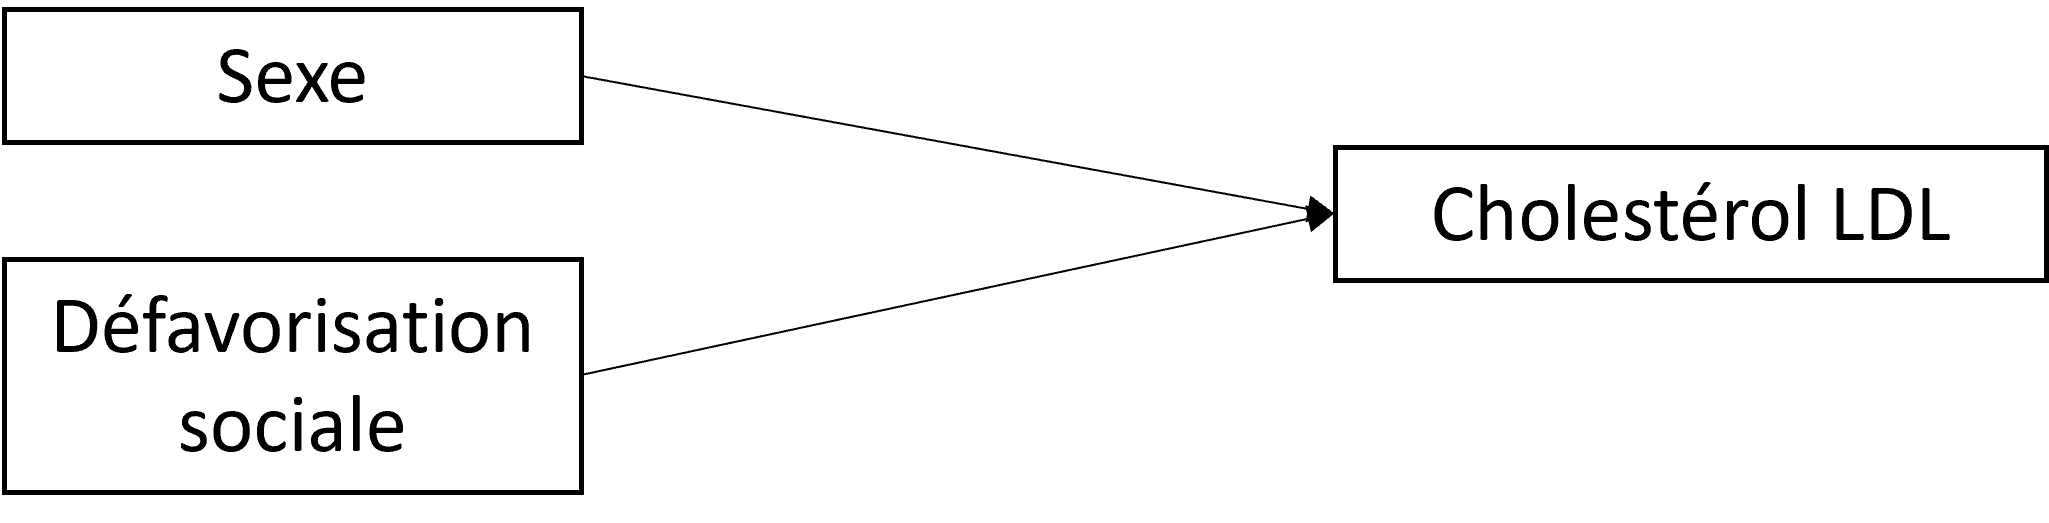
\includegraphics[width=0.5\textwidth,height=\textheight]{img/Image13.png}
\end{quote}

\textbf{Les estimands} étaient définis sur l'échelle additive par :

\begin{itemize}
\tightlist
\item
  La modification de l'effet du sexe en fonction par la défavorisation sociale précoce :

  \begin{itemize}
  \tightlist
  \item
    \(\small (Y_{s=1|d=0} - Y_{s=0|d=0}) - (Y_{s=1|d=1} - Y_{s=0|d=1})\)
  \item
    ou \(\small (Y_{s=1,d=0} - Y_{s=0,d=0}) - (Y_{s=1,d=1} - Y_{s=0,d=1})\)
  \end{itemize}
\item
  La modification de l'effet de la défavorisation sociale précoce par la sexe

  \begin{itemize}
  \tightlist
  \item
    \(\small (Y_{d=1|s=0} - Y_{d=0|s=0}) - (Y_{d=1|s=1} - Y_{d=0|s=1})\)
  \item
    ou \(\small (Y_{d=1,s=0} - Y_{d=0,s=0}) - (Y_{d=1,s=1} - Y_{d=0,s=1})\)
  \end{itemize}
\end{itemize}

Les deux formulations sont ici équivalentes car il n'y pas de facteurs de confusion, donc, par exemple, \(\small Y_{d=1|s=0} = Y_{s=0|d=1} = Y_{d=1,s=0}\)

\textbf{L'estimateur} :
Les effets ont été estimés par g-computation (\emph{standardisation par régression}) \citet{hernan2020causal}.
Des régressions linéaires ont été utilisées pour estimer les \emph{potential outcomes} pour chaque scénario, désignées par \(\small \overline{Q}(S, D) = E(Y|S, D)\).
A partir des fonctions \(\small \overline{Q}(S, D)\) estimées, nous avons prédit la valeur de l'outcome Y pour chaque individu i pour chaque scénario. Les valeurs moyennes de Y dans chaque scénario vont ensuite nous permettre d'estimer les estimands selon leurs définitions précisées ci-dessus.
Ces modèles\(\small \overline{Q}(S, D)\) vont comprendre 2 variables : le sexe et la défavorisation sociale précoce (il n'y a pas ici de facteurs de confusion).

\hypertarget{analyse-descriptive}{%
\section{Analyse descriptive}\label{analyse-descriptive}}

Dans cette population (N=17 272), il y avait 51,4\% d'hommes et 60,5\% de personnes ayant été précocement défavorisées.

On peut commencer par décrire les moyennes de cholestérol dans chaque catégorie de sexe et de défavorisation sociale :

\begin{table}
\centering
\begin{tabular}[t]{l|l|l}
\hline
Sexe & Défavorisation & Mean(Chol LDL)\\
\hline
Male & Non & 3.57\\
\hline
Male & Oui & 3.60\\
\hline
Female & Non & 3.24\\
\hline
Female & Oui & 3.37\\
\hline
\end{tabular}
\end{table}

\hypertarget{analyse-exploratoire}{%
\section{Analyse exploratoire}\label{analyse-exploratoire}}

La sortie d'une modèle linéaire simple serait :

\begin{Shaded}
\begin{Highlighting}[]
\CommentTok{\# Call:}
\CommentTok{\# lm(formula = t8\_ldl \textasciitilde{} as.factor(sex) + as.factor(soc\_group) + }
\CommentTok{\#     as.factor(sex) * as.factor(soc\_group), data = ba\_1)}
\CommentTok{\# }
\CommentTok{\# Coefficients:}
\CommentTok{\#                                             Estimate Std. Error t value Pr(\textgreater{}|t|)    }
\CommentTok{\# (Intercept)                                  3.24270    0.01594 203.475  \textless{} 2e{-}16 ***}
\CommentTok{\# as.factor(sex)1                              0.32553    0.02227  14.616  \textless{} 2e{-}16 ***}
\CommentTok{\# as.factor(soc\_group)2.Défav                  0.12614    0.02052   6.148 8.02e{-}10 ***}
\CommentTok{\# as.factor(sex)1:as.factor(soc\_group)2.Défav {-}0.09473    0.02863  {-}3.308 0.000941 ***}
\CommentTok{\# {-}{-}{-}}
\CommentTok{\# Signif. codes:  0 ‘***’ 0.001 ‘**’ 0.01 ‘*’ 0.05 ‘.’ 0.1 ‘ ’ 1}
\CommentTok{\# }
\end{Highlighting}
\end{Shaded}

On peut en déduire (échelle additive) que :

\begin{itemize}
\tightlist
\item
  L'effet du sexe (d'être homme plutot que femme) est :

  \begin{itemize}
  \tightlist
  \item
    Quand on est favorisé : \(\small DR(S|D=0) = +0.326\) mmol/L
  \item
    Quand on est défavorisé : \(\small DR(S|D=1) = 0.326 - 0.095 =\) +0.231 mmol/L
  \end{itemize}
\item
  L'effet de la défavorisation est :

  \begin{itemize}
  \tightlist
  \item
    Quand on est une femme : \(\small DR(D|S=0) = +0.126\) mmol/L
  \item
    Quand on est un homme : \(\small DR(D|S=1) = 0.126 - 0.095 =\) +0.031 mmol/L
  \end{itemize}
\item
  L'effet d'être un homme et défavorisé

  \begin{itemize}
  \tightlist
  \item
    plutot que femme et favorisé est
  \item
    \(\small DR(D,S) = 0.326 + 0.126 - 0.095 =\) +0.357 mmol/L
  \end{itemize}
\item
  \textbf{L'effet d'interaction/modification d'effet} est : \(\small AI = -0.095\) mmol/L
\end{itemize}

On pourrait aussi déduire :

\begin{itemize}
\tightlist
\item
  \(\small Y_{00} = 3.24\) mmol/L
\item
  \(\small Y_{10} = 3.243 + 0.326 =\) 3.57 mmol/L
\item
  \(\small Y_{01} = 3.243 + 0.126 =\) 3.37 mmol/L
\item
  \(\small Y_{11} = 3.243 + 0.326 + 0.126 - 0.095 =\) 3.6 mmol/L
\end{itemize}

\hypertarget{analyse-confirmatoire}{%
\section{Analyse confirmatoire}\label{analyse-confirmatoire}}

Si l'on utilise le \href{https://github.com/benoitlepage/MargIntTmle}{package proposé par B Lepage} pour réaliser cet analyse avec la TMLE (effets d'intéraction calculés à partir des paramètres d'une modèle structurel marginal estimé à l'aide du package R ltmle), les résultats sont :

\begin{table}
\centering
\begin{tabular}{l|l|l|l}
\hline
  & A2=0 & A2=1 & RD.A2|A1\\
\hline
A1=0 & \$p\_\{00\}\$=3.243 [3.213,3.273] & \$p\_\{01\}\$=3.369 [3.344,3.394] & 0.126 [0.087,0.165]\\
\hline
A1=1 & \$p\_\{10\}\$=3.568 [3.538,3.598] & \$p\_\{11\}\$=3.6 [3.574,3.625] & 0.031 [-0.008,0.071]\\
\hline
RD.A1|A2 & 0.326 [0.283,0.368] & 0.231 [0.195,0.267] & \\
\hline
\multicolumn{4}{l}{\textsuperscript{a} additive Interaction = -0.095 [-0.15;-0.039]}\\
\end{tabular}
\end{table}

On retrouve des résulats qui peuvent être intérprétés ainsi :

\begin{itemize}
\tightlist
\item
  l'effet d'être un homme (ou ``la différence H-F) est moins fort de additive Interaction = -0.095 {[}-0.15;-0.039{]} mmol/L lorsqu'on est défavorisé précocement
\item
  l'effet de la défavorisation est moins fort de additive Interaction = -0.095 {[}-0.15;-0.039{]} mmol/L chez les hommes
\end{itemize}

\begin{center}\rule{0.5\linewidth}{0.5pt}\end{center}

En réalité, on a réalisé cette analyse par g-computation (voir chapitre \ref{conf}) sur des données imputées et boostrappées (l'exemple ci-dessus a été réalisé sur une seule des bases bootstrappées, ce qui explique les différences), et les résultats, présentées selon les recommandations modifiées de Knol et VanderWeele, étaient:

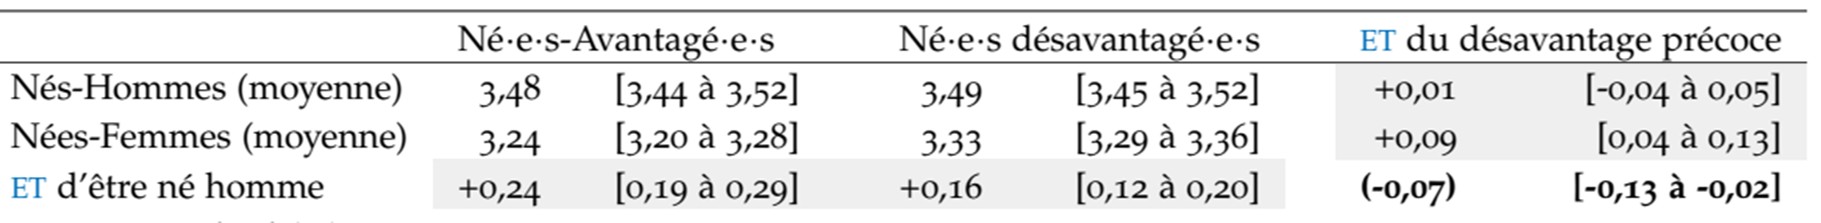
\includegraphics[width=1\textwidth,height=\textheight]{img/result_quanti.png}

\hypertarget{exemple-3---y-multinomial}{%
\chapter{Exemple 3 - Y multinomial}\label{exemple-3---y-multinomial}}

\hypertarget{exemple-4---x-quantitatif}{%
\chapter{Exemple 4 - X quantitatif}\label{exemple-4---x-quantitatif}}

Les articles qui se consacrent aux interactions présentent souvent des méthodes applicables lorsque les deux expositions X et V sont binaires. Or, en épidémiologie, les expositions peuvent aussi être continues et, si dichotomiser ces variables peut simplifier l'approche de l'interaction, cela conduit à une perte d'information qui n'est pas souhaitable et pose la question complexe du choix des seuils \citet{royston2006dichotomizing} \citet{knol2007estimating} \citet{cadarso2006effect}.

Nous présentons ici un exemple dans lequel l'une des expositions, l'âge, est analysée en tant que variable quantitative continue.

\hypertarget{formuler-les-objectifs-1}{%
\section{Formuler les objectifs}\label{formuler-les-objectifs-1}}

Dans cette étude fictive, on s'est intéressé à la consommation de cannabis : comment le fait d'avoir déjà fumé du cannabis Y varie avec l'âge A et le sexe S.

La démarche est explicative : on cherche à comprendre les mécanismes causaux de ce comportement de santé.

Ici, on adoptera une démarche d'analyse d'interaction \(\small do(S,A)\)

\hypertarget{stratuxe9gies-et-muxe9thodes-1}{%
\section{Stratégies et méthodes}\label{stratuxe9gies-et-muxe9thodes-1}}

\textbf{Le DAG} (sans les médiateurs) était :

\begin{quote}
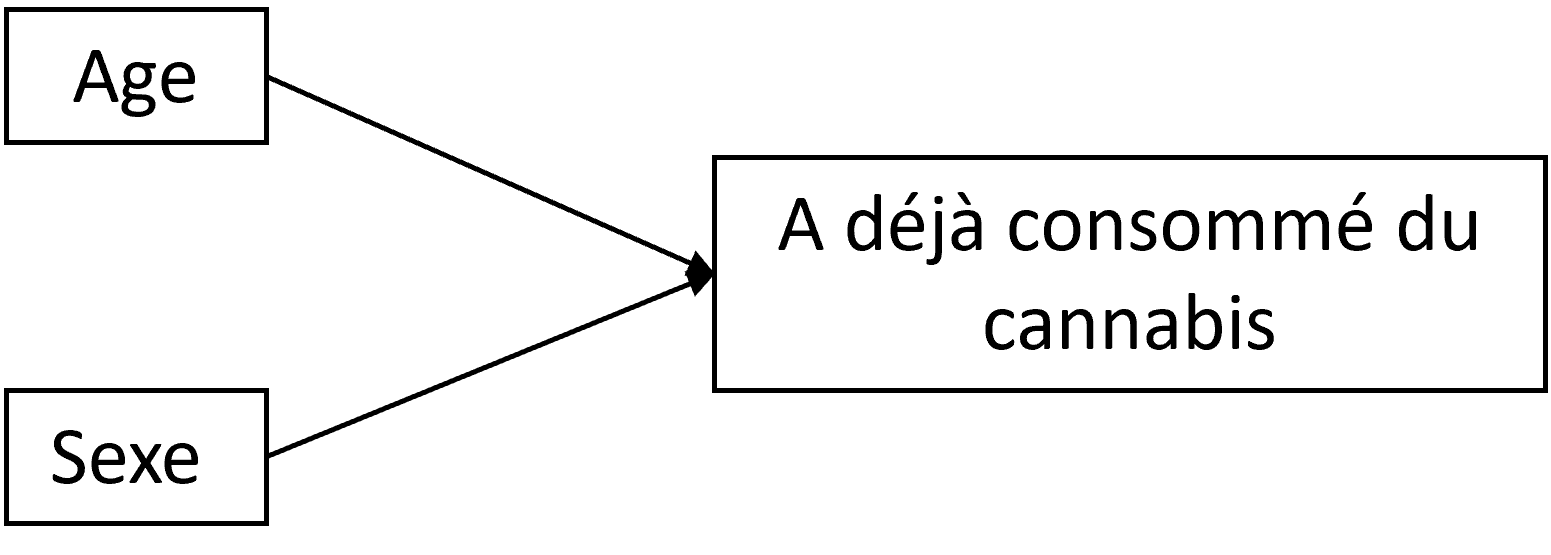
\includegraphics[width=0.5\textwidth,height=\textheight]{img/Image14.png}
\end{quote}

\textbf{Les estimands} était définis par :

\begin{itemize}
\tightlist
\item
  L'effet de l'âge (``avoir 10 ans de plus'') chez les hommes

  \begin{itemize}
  \tightlist
  \item
    \(\small DR = Y_{S=0,A=a+10} - Y_{S=0,A=a}\)
  \item
    \(\small RR = \frac{Y_{S=0,A=a+10}}{Y_{S=0,A=a}}\)
  \end{itemize}
\item
  L'effet de l'âge (``avoir 10 ans de plus'') chez les femmes :

  \begin{itemize}
  \tightlist
  \item
    \(\small DR = Y_{S=1,A=a+10} - Y_{S=1,A=a}\)
  \item
    \(\small RR = \frac{Y_{S=1,A=a+10}}{Y_{S=1,A=a}}\)
  \end{itemize}
\item
  L'effet d'interaction entre l'âge et le sexe (l'effet du sexe est-il différent en fonction de l'âge et l'effet de l'âge est-il différent en fonction du sexe ?)

  \begin{itemize}
  \tightlist
  \item
    sur l'échelle additive : \(\small AI = Y_{S=1,A=a+10} - Y_{S=0,A=a+10} - Y_{S=1,A=a} + Y_{S=0,A=a+10}\)
  \item
    sur l'échelle multiplicative : \(\small MI =\frac{Y_{S=1,A=a+10} \times Y_{S=0,A=a}}{Y_{S=1,A=a} \times Y_{S=0,A=a+10}}\)
  \end{itemize}
\end{itemize}

\hypertarget{analyse-descriptive-1}{%
\section{Analyse descriptive}\label{analyse-descriptive-1}}

Dans cette population (N=202 768), il y avait 53,7\% d'hommes et la moyenne d'âge était de 47,1 ans.

On peut commencer par décrire la proportion de personnes ayant déjà fumé du cannabis par sexe et classe d'âge :

\begin{table}
\centering
\begin{tabular}[t]{l|l|l}
\hline
Sexe & Age & P(Cannabis), \%\\
\hline
Male & 20- & 51,1\\
\hline
Male & ]20 à 40] & 66,3\\
\hline
Male & ]40 à 60] & 40,4\\
\hline
Male & 60+ & 12,1\\
\hline
Female & 20- & 44,2\\
\hline
Female & ]20 à 40] & 52,7\\
\hline
Female & ]40 à 60] & 26,7\\
\hline
Female & 60+ & 12,1\\
\hline
\end{tabular}
\end{table}

Il semble y avoir une interaction entre l'âge et le sexe sur la probabilité d'avoir déjà fumé du cannabis. Cependant, la relation entre l'âge et l'outcome ne semble pas linéaire, ce qui est confirmé graphiquement :

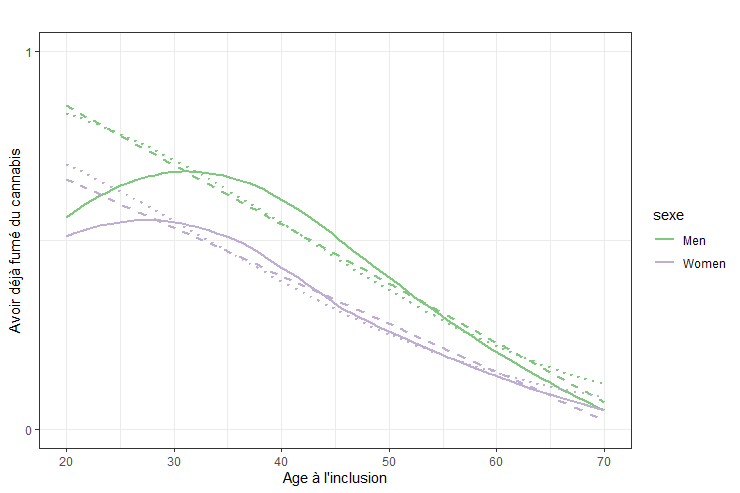
\includegraphics[width=0.8\textwidth,height=\textheight]{img/graph_Xquanti_1.png}

Pour simplifier les analyses, nous n'allons inclure que les plus de 30 ans (N = 177 940), pour lesquels la relation est linéaire :

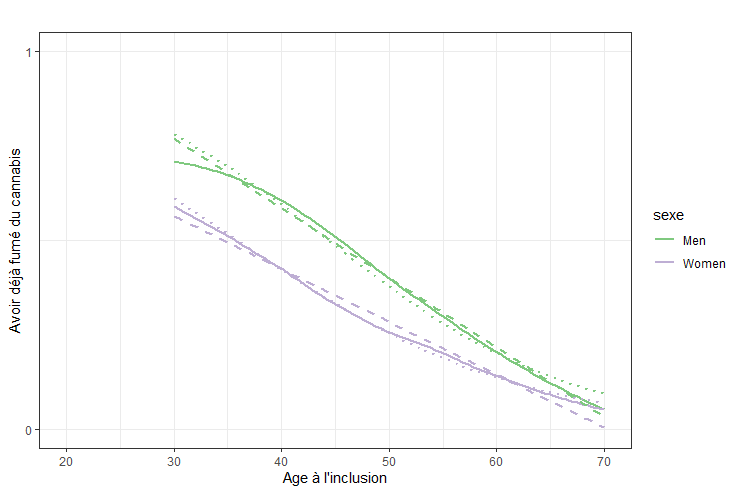
\includegraphics[width=0.8\textwidth,height=\textheight]{img/graph_Xquanti_2.png}

Le modèle de régression logistique (\(\cdot\cdot\cdot\)) semble être plus proche de la modélisation non paramétrique sur données observées (loess, -----) que la modélisation linaire (\(---\)) . D'ailleurs, le R² du modèle logistique est de 0,168 contre 0,139 pour le modèle linéaire.

\hypertarget{analyse-exploratoire-1}{%
\section{Analyse exploratoire}\label{analyse-exploratoire-1}}

\hypertarget{ruxe9gression-logistique-1}{%
\subsection{Régression logistique}\label{ruxe9gression-logistique-1}}

L'outcome étant binaire, il est plus classique d'utiliser un modèle logistique, dont les résultats seraient :

\begin{Shaded}
\begin{Highlighting}[]
\CommentTok{\# Call:}
\CommentTok{\# glm(formula = cannabis \textasciitilde{} sexe + age + sexe * age, family = binomial, }
\CommentTok{\#     data = data)}
\CommentTok{\# }
\CommentTok{\# Coefficients:}
\CommentTok{\#                 Estimate Std. Error z value Pr(\textgreater{}|z|)    }
\CommentTok{\# (Intercept)    3.9144609  0.0372560  105.07   \textless{}2e{-}16 ***}
\CommentTok{\# sexeWomen     {-}1.1644706  0.0511834  {-}22.75   \textless{}2e{-}16 ***}
\CommentTok{\# age           {-}0.0882928  0.0007566 {-}116.70   \textless{}2e{-}16 ***}
\CommentTok{\# sexeWomen:age  0.0117238  0.0010623   11.04   \textless{}2e{-}16 ***}
\CommentTok{\# {-}{-}{-}}
\CommentTok{\# Signif. codes:  0 ‘***’ 0.001 ‘**’ 0.01 ‘*’ 0.05 ‘.’ 0.1 ‘ ’ 1}
\end{Highlighting}
\end{Shaded}

Ce qui, en terme d'OR, donnerait :

\begin{Shaded}
\begin{Highlighting}[]
\CommentTok{\#                       OR      2.5 \%     97.5 \%}
\CommentTok{\# (Intercept)   50.1220409 46.5985990 53.9259952}
\CommentTok{\# sexeWomen      0.3120878  0.2822910  0.3450107}
\CommentTok{\# age            0.9154927  0.9141333  0.9168485}
\CommentTok{\# sexeWomen:age  1.0117927  1.0096884  1.0139018}
\end{Highlighting}
\end{Shaded}

Les modèles de régression logistique donnent des résulats sur l'échelle multiplicative :

\begin{itemize}
\tightlist
\item
  L'effet du sexe (d'être femme plutot que homme) est :

  \begin{itemize}
  \tightlist
  \item
    ``A 0 ans'' (à l'origine) : \(\small OR(S|A=0) = \times 0.31\)
  \item
    ``A 1 ans'' : \(\small OR(S|A=1) = exp(-1,164 + 0,012) \times\) 0.32
  \item
    A 40 ans (par exemple) : \(\small OR(S|A=40) = exp(-1,164 + 0,012 \times 40) = \times\) 0.5
  \end{itemize}
\item
  L'effet de l'age est :

  \begin{itemize}
  \tightlist
  \item
    Quand on est un homme : \(\small OR(A|S=0) = exp(-0,088\times 10 ) = \times\) 0.41 par 10 ans
  \item
    Quand on est une femme : \(\small OR(A|S=1) = exp(-0,088\times 10 + 0,012\times 10) = \times\) 0.47 par 10 ans
  \end{itemize}
\item
  L'effet d'être une femme et d'avoir 10 ans de plus

  \begin{itemize}
  \tightlist
  \item
    plutot que homme ``et 0 ans''
  \item
    \(\small OR(A,S) = exp(-1,164 -0,088\times 10 + 0,012\times 10) = \times\) 0.15
  \end{itemize}
\item
  \textbf{L'effet d'interaction/modification d'effet} est :

  \begin{itemize}
  \tightlist
  \item
    \(\small MI =\times 1,01\) sur 1 an
  \item
    \(\small MI_{10} = exp(0,012\times 10 ) = \times\) 1.13 sur 10 ans
  \end{itemize}
\item
  \textbf{Un effet d'interaction additif}

  \begin{itemize}
  \tightlist
  \item
    \(\small RERI_{OR} = OR_{11} - OR_{01} - OR_{10} + 1 =\) 0.047 pour 1 ans
  \item
    \(\small RERI_{OR,10} =\) 0.362
  \end{itemize}
\end{itemize}

On a donc une interaction multiplicative positive (MI\textgreater1) et significative et une interaction additive aussi positive (RERI \textgreater0).

\hypertarget{ruxe9gression-linuxe9aire}{%
\subsection{Régression linéaire}\label{ruxe9gression-linuxe9aire}}

La sortie d'une modèle linéaire simple serait :

\begin{Shaded}
\begin{Highlighting}[]
\CommentTok{\# }
\CommentTok{\# Call:}
\CommentTok{\# lm(formula = cannabis \textasciitilde{} sexe + age + sexe * age, data = data)}
\CommentTok{\# }
\CommentTok{\# Coefficients:}
\CommentTok{\#                 Estimate Std. Error t value Pr(\textgreater{}|t|)    }
\CommentTok{\# (Intercept)    1.3197103  0.0066820  197.50   \textless{}2e{-}16 ***}
\CommentTok{\# sexeWomen     {-}0.3373482  0.0091573  {-}36.84   \textless{}2e{-}16 ***}
\CommentTok{\# age           {-}0.0183730  0.0001294 {-}142.03   \textless{}2e{-}16 ***}
\CommentTok{\# sexeWomen:age  0.0044248  0.0001781   24.85   \textless{}2e{-}16 ***}
\CommentTok{\# Signif. codes:  0 ‘***’ 0.001 ‘**’ 0.01 ‘*’ 0.05 ‘.’ 0.1 ‘ ’ 1}
\end{Highlighting}
\end{Shaded}

On peut en déduire, ici sur une échelle additive, que :

\begin{itemize}
\tightlist
\item
  L'effet du sexe (d'être femme plutot que homme) est :

  \begin{itemize}
  \tightlist
  \item
    ``A 0 ans'' (à l'origine) : \(\small DR(S|A=0) = -33,73\)\%
  \item
    A 20 ans (par exemple) : \(\small DR(S|A=20) = -33,73 + 0,44 \times 20 =\) -24.93\%
  \item
    A 40 ans (par exemple) : \(\small DR(S|A=40) = -33,73 + 0,44 \times 40 =\) -16.13\%
  \item
    A 60 ans (par exemple) : \(\small DR(S|A=60) = -33,73 + 0,44 \times 60 =\) -7.33\%
  \end{itemize}
\item
  L'effet de l'age est :

  \begin{itemize}
  \tightlist
  \item
    Quand on est un homme : \(\small DR(A|S=0) = -1,84\times 10 =\) -18.4\% par 10 ans
  \item
    Quand on est une femme : \(\small DR(A|S=1) = -1,84\times 10 + 0.44\times 10 =\) -14 \% par année d'âge
  \end{itemize}
\item
  L'effet d'être une femme et d'avoir 10 ans de plus

  \begin{itemize}
  \tightlist
  \item
    plutot que homme et un certain âge
  \item
    \(\small DR(A,S) = -33,73 -1,84\times 10 + 0,44\times 10 =\) -47.73 \%
  \end{itemize}
\item
  \textbf{L'effet d'interaction/modification d'effet} est :

  \begin{itemize}
  \tightlist
  \item
    \(\small AI = +0.44\)`\%
  \item
    \(\small AI_{10} = +0.44\times 10 =\) 4.4\%
  \end{itemize}
\end{itemize}

On retrouve une interaction additive significative et positive. Les expositions ayant un effet négatif et l'effet d'interaction étant positif, cet effet est difficile à interpréter, mais on pourrait le formuler plus simplement en changeant la catégorie de référence du sexe de homme à femme.

Ainsi : globalement, la probabilité d'avoir déjà fumer du cannabis diminue avec l'âge chez les hommes (-1,8\% par an) et chez les femmes (-1,4\% par an). Cette probabilité est plus élevée chez les hommes (de 16\% par exemple à 40 ans), mais cet écart diminue avec l'âge, de 4,4\% tous les 10 ans.

\hypertarget{effets-marginaux}{%
\subsection{Effets marginaux}\label{effets-marginaux}}

A partir des modèles, on peut déduire les effets marginaux pour certaines catégories. Par exemple, avec le modèle logistique :

\begin{itemize}
\tightlist
\item
  \(\small Y_{S=0,A=30} = \frac{exp(3,914 - 0,088 \times 30)}{1+exp(3,914 - 0,088 \times 30)} =\) 78.1\%
\item
  \(\small Y_{S=0,A=50} = \frac{exp(3,914 - 0,088 \times 50)}{1+exp(3,914 - 0,088 \times 50)} =\) 38.1\%
\item
  \(\small Y_{S=1,A=30} = \frac{exp(3,914 - 1,164 - 0,088 \times 30 + 0,012 \times 30)}{1+exp(3,914 - 1,164 - 0,088 \times 30 + 0,012 \times 30)} =\) 61.5\%
\item
  \(\small Y_{S=1,A=50} = \frac{exp(3,914 - 1,164 - 0,088 \times 50 + 0,012 \times 50)}{1+exp(3,914 - 1,164 - 0,088 \times 50 + 0,012 \times 50)} =\) 25.9\%
\end{itemize}

Avec le modèle linéaire, on aurait :

\begin{itemize}
\tightlist
\item
  \(\small Y_{S=0,A=30} = 131,97 - 1,84 \times 30 =\) 76.8\%
\item
  \(\small Y_{S=0,A=50} = 131,97 - 1,84 \times 50 =\) 40\%
\item
  \(\small Y_{S=1,A=30} = 131,97 -33,73 - 1,84 \times 30 + 0,44 \times 30 =\) 56.2\%
\item
  \(\small Y_{S=1,A=50} = 131,97 -33,73 - 1,84 \times 50 + 0,44 \times 50 =\) 28.2\%
\end{itemize}

\hypertarget{analyse-confirmatoire-1}{%
\section{Analyse confirmatoire}\label{analyse-confirmatoire-1}}

Nous avons calculé les effets d'intérêt avec une méthode de modèle structurel marginal (Intervalles de confiance estimé par bootstrap, 200 répétitions), le modèle utilisé pour prédire les outcomes contrefactuels étaient un modèle de régression logistique.

Le code était :

\begin{Shaded}
\begin{Highlighting}[]
\NormalTok{     B}\OtherTok{=}\DecValTok{200}
     
\NormalTok{     simu.base }\OtherTok{\textless{}{-}} \FunctionTok{data.frame}\NormalTok{(}\AttributeTok{i.simu=}\FunctionTok{c}\NormalTok{(}\DecValTok{1}\SpecialCharTok{:}\NormalTok{B))}
     
     \ControlFlowTok{for}\NormalTok{ (i }\ControlFlowTok{in} \DecValTok{1}\SpecialCharTok{:}\NormalTok{B)\{ }
       \CommentTok{\# sample the indices 1 to n with replacement}
\NormalTok{       bootIndices }\OtherTok{\textless{}{-}} \FunctionTok{sample}\NormalTok{(}\DecValTok{1}\SpecialCharTok{:}\FunctionTok{nrow}\NormalTok{(data), }\AttributeTok{replace=}\NormalTok{T) ;    }\FunctionTok{set.seed}\NormalTok{(}\DecValTok{01062023}\SpecialCharTok{+}\NormalTok{i}\SpecialCharTok{*}\DecValTok{12}\NormalTok{)}
\NormalTok{       bootData }\OtherTok{\textless{}{-}}\NormalTok{ data[bootIndices,]}
       
       \CommentTok{\#modèle}
\NormalTok{       Q.model }\OtherTok{\textless{}{-}} \FunctionTok{glm}\NormalTok{(}\AttributeTok{data=}\NormalTok{bootData, }\AttributeTok{formula =}\NormalTok{ cannabis }\SpecialCharTok{\textasciitilde{}}\NormalTok{ sexe}\SpecialCharTok{+}
\NormalTok{                        age}\SpecialCharTok{+}\NormalTok{  sexe}\SpecialCharTok{*}\NormalTok{age,}\AttributeTok{family =}\NormalTok{ binomial)}
       
       \CommentTok{\# Scénarios \#}
\NormalTok{       data.S1 }\OtherTok{\textless{}{-}}\NormalTok{  data.S2 }\OtherTok{\textless{}{-}}\NormalTok{ predict\_data}
\NormalTok{       data.S1}\SpecialCharTok{$}\NormalTok{sexe }\OtherTok{\textless{}{-}} \StringTok{"Women"}
\NormalTok{       data.S2}\SpecialCharTok{$}\NormalTok{sexe }\OtherTok{\textless{}{-}} \StringTok{"Men"}
\NormalTok{       data.S1A30 }\OtherTok{\textless{}{-}}\NormalTok{  data.S1A40 }\OtherTok{\textless{}{-}}\NormalTok{ data.S1A50 }\OtherTok{\textless{}{-}}\NormalTok{ data.S1A60 }\OtherTok{\textless{}{-}}\NormalTok{ data.S1A70 }\OtherTok{\textless{}{-}}\NormalTok{ data.S1}
\NormalTok{       data.S1A35 }\OtherTok{\textless{}{-}}\NormalTok{  data.S1A45 }\OtherTok{\textless{}{-}}\NormalTok{ data.S1A55 }\OtherTok{\textless{}{-}}\NormalTok{ data.S1A65 }\OtherTok{\textless{}{-}}\NormalTok{ data.S1}
\NormalTok{       data.S2A30 }\OtherTok{\textless{}{-}}\NormalTok{  data.S2A40 }\OtherTok{\textless{}{-}}\NormalTok{ data.S2A50 }\OtherTok{\textless{}{-}}\NormalTok{ data.S2A60 }\OtherTok{\textless{}{-}}\NormalTok{ data.S2A70 }\OtherTok{\textless{}{-}}\NormalTok{ data.S2}
\NormalTok{       data.S2A35 }\OtherTok{\textless{}{-}}\NormalTok{  data.S2A45 }\OtherTok{\textless{}{-}}\NormalTok{ data.S2A55 }\OtherTok{\textless{}{-}}\NormalTok{ data.S2A65 }\OtherTok{\textless{}{-}}\NormalTok{ data.S2}
\NormalTok{       data.S1A30}\SpecialCharTok{$}\NormalTok{age }\OtherTok{\textless{}{-}}\NormalTok{ data.S2A30}\SpecialCharTok{$}\NormalTok{age }\OtherTok{\textless{}{-}} \DecValTok{30}
\NormalTok{       data.S1A35}\SpecialCharTok{$}\NormalTok{age }\OtherTok{\textless{}{-}}\NormalTok{ data.S2A35}\SpecialCharTok{$}\NormalTok{age }\OtherTok{\textless{}{-}} \DecValTok{35}
\NormalTok{       data.S1A40}\SpecialCharTok{$}\NormalTok{age }\OtherTok{\textless{}{-}}\NormalTok{ data.S2A40}\SpecialCharTok{$}\NormalTok{age }\OtherTok{\textless{}{-}} \DecValTok{40}
\NormalTok{       data.S1A45}\SpecialCharTok{$}\NormalTok{age }\OtherTok{\textless{}{-}}\NormalTok{ data.S2A45}\SpecialCharTok{$}\NormalTok{age }\OtherTok{\textless{}{-}} \DecValTok{45}
\NormalTok{       data.S1A50}\SpecialCharTok{$}\NormalTok{age }\OtherTok{\textless{}{-}}\NormalTok{ data.S2A50}\SpecialCharTok{$}\NormalTok{age }\OtherTok{\textless{}{-}} \DecValTok{50}
\NormalTok{       data.S1A55}\SpecialCharTok{$}\NormalTok{age }\OtherTok{\textless{}{-}}\NormalTok{ data.S2A55}\SpecialCharTok{$}\NormalTok{age }\OtherTok{\textless{}{-}} \DecValTok{55}
\NormalTok{       data.S1A60}\SpecialCharTok{$}\NormalTok{age }\OtherTok{\textless{}{-}}\NormalTok{ data.S2A60}\SpecialCharTok{$}\NormalTok{age }\OtherTok{\textless{}{-}} \DecValTok{60}
\NormalTok{       data.S1A65}\SpecialCharTok{$}\NormalTok{age }\OtherTok{\textless{}{-}}\NormalTok{ data.S2A65}\SpecialCharTok{$}\NormalTok{age }\OtherTok{\textless{}{-}} \DecValTok{65}
\NormalTok{       data.S1A70}\SpecialCharTok{$}\NormalTok{age }\OtherTok{\textless{}{-}}\NormalTok{ data.S2A70}\SpecialCharTok{$}\NormalTok{age }\OtherTok{\textless{}{-}} \DecValTok{70}
       
       
       \CommentTok{\# Y contrefactuel}
\NormalTok{       Y.S1A30.pred }\OtherTok{\textless{}{-}} \FunctionTok{predict}\NormalTok{(Q.model, }\AttributeTok{newdata =}\NormalTok{ data.S1A30, }\AttributeTok{type =} \StringTok{"response"}\NormalTok{)}
\NormalTok{       Y.S1A40.pred }\OtherTok{\textless{}{-}} \FunctionTok{predict}\NormalTok{(Q.model, }\AttributeTok{newdata =}\NormalTok{ data.S1A40, }\AttributeTok{type =} \StringTok{"response"}\NormalTok{)}
\NormalTok{       Y.S1A50.pred }\OtherTok{\textless{}{-}} \FunctionTok{predict}\NormalTok{(Q.model, }\AttributeTok{newdata =}\NormalTok{ data.S1A50, }\AttributeTok{type =} \StringTok{"response"}\NormalTok{)}
\NormalTok{       Y.S1A60.pred }\OtherTok{\textless{}{-}} \FunctionTok{predict}\NormalTok{(Q.model, }\AttributeTok{newdata =}\NormalTok{ data.S1A60, }\AttributeTok{type =} \StringTok{"response"}\NormalTok{)}
\NormalTok{       Y.S1A70.pred }\OtherTok{\textless{}{-}} \FunctionTok{predict}\NormalTok{(Q.model, }\AttributeTok{newdata =}\NormalTok{ data.S1A70, }\AttributeTok{type =} \StringTok{"response"}\NormalTok{)}
\NormalTok{       Y.S2A30.pred }\OtherTok{\textless{}{-}} \FunctionTok{predict}\NormalTok{(Q.model, }\AttributeTok{newdata =}\NormalTok{ data.S2A30, }\AttributeTok{type =} \StringTok{"response"}\NormalTok{)}
\NormalTok{       Y.S2A40.pred }\OtherTok{\textless{}{-}} \FunctionTok{predict}\NormalTok{(Q.model, }\AttributeTok{newdata =}\NormalTok{ data.S2A40, }\AttributeTok{type =} \StringTok{"response"}\NormalTok{)}
\NormalTok{       Y.S2A50.pred }\OtherTok{\textless{}{-}} \FunctionTok{predict}\NormalTok{(Q.model, }\AttributeTok{newdata =}\NormalTok{ data.S2A50, }\AttributeTok{type =} \StringTok{"response"}\NormalTok{)}
\NormalTok{       Y.S2A60.pred }\OtherTok{\textless{}{-}} \FunctionTok{predict}\NormalTok{(Q.model, }\AttributeTok{newdata =}\NormalTok{ data.S2A60, }\AttributeTok{type =} \StringTok{"response"}\NormalTok{)}
\NormalTok{       Y.S2A70.pred }\OtherTok{\textless{}{-}} \FunctionTok{predict}\NormalTok{(Q.model, }\AttributeTok{newdata =}\NormalTok{ data.S2A70, }\AttributeTok{type =} \StringTok{"response"}\NormalTok{)}
       
\NormalTok{       Y.S1A35.pred }\OtherTok{\textless{}{-}} \FunctionTok{predict}\NormalTok{(Q.model, }\AttributeTok{newdata =}\NormalTok{ data.S1A35, }\AttributeTok{type =} \StringTok{"response"}\NormalTok{)}
\NormalTok{       Y.S1A45.pred }\OtherTok{\textless{}{-}} \FunctionTok{predict}\NormalTok{(Q.model, }\AttributeTok{newdata =}\NormalTok{ data.S1A45, }\AttributeTok{type =} \StringTok{"response"}\NormalTok{)}
\NormalTok{       Y.S1A55.pred }\OtherTok{\textless{}{-}} \FunctionTok{predict}\NormalTok{(Q.model, }\AttributeTok{newdata =}\NormalTok{ data.S1A55, }\AttributeTok{type =} \StringTok{"response"}\NormalTok{)}
\NormalTok{       Y.S1A65.pred }\OtherTok{\textless{}{-}} \FunctionTok{predict}\NormalTok{(Q.model, }\AttributeTok{newdata =}\NormalTok{ data.S1A65, }\AttributeTok{type =} \StringTok{"response"}\NormalTok{)}
\NormalTok{       Y.S2A35.pred }\OtherTok{\textless{}{-}} \FunctionTok{predict}\NormalTok{(Q.model, }\AttributeTok{newdata =}\NormalTok{ data.S2A35, }\AttributeTok{type =} \StringTok{"response"}\NormalTok{)}
\NormalTok{       Y.S2A45.pred }\OtherTok{\textless{}{-}} \FunctionTok{predict}\NormalTok{(Q.model, }\AttributeTok{newdata =}\NormalTok{ data.S2A45, }\AttributeTok{type =} \StringTok{"response"}\NormalTok{)}
\NormalTok{       Y.S2A55.pred }\OtherTok{\textless{}{-}} \FunctionTok{predict}\NormalTok{(Q.model, }\AttributeTok{newdata =}\NormalTok{ data.S2A55, }\AttributeTok{type =} \StringTok{"response"}\NormalTok{)}
\NormalTok{       Y.S2A65.pred }\OtherTok{\textless{}{-}} \FunctionTok{predict}\NormalTok{(Q.model, }\AttributeTok{newdata =}\NormalTok{ data.S2A65, }\AttributeTok{type =} \StringTok{"response"}\NormalTok{)}

\NormalTok{       Y }\OtherTok{\textless{}{-}} \FunctionTok{c}\NormalTok{(Y.S1A30.pred, Y.S1A40.pred, Y.S1A50.pred, Y.S1A60.pred, Y.S1A70.pred,}
\NormalTok{              Y.S1A35.pred, Y.S1A45.pred, Y.S1A55.pred, Y.S1A65.pred,}
\NormalTok{              Y.S2A30.pred, Y.S2A40.pred, Y.S2A50.pred, Y.S2A60.pred, Y.S2A70.pred,}
\NormalTok{              Y.S2A35.pred, Y.S2A45.pred, Y.S2A55.pred, Y.S2A65.pred)}
       
     \CommentTok{\# On récupère les valeurs d\textquotesingle{}exposition qui ont servi dans les scénarios contrefactuels}
     \CommentTok{\# (garder le même ordre que pour les Y.A1.A2)}
       
\NormalTok{     X }\OtherTok{\textless{}{-}} \FunctionTok{rbind}\NormalTok{(}\FunctionTok{subset}\NormalTok{(data.S1A30, }\AttributeTok{select =} \FunctionTok{c}\NormalTok{(}\StringTok{"sexe"}\NormalTok{, }\StringTok{"age"}\NormalTok{)),}
                \FunctionTok{subset}\NormalTok{(data.S1A40, }\AttributeTok{select =} \FunctionTok{c}\NormalTok{(}\StringTok{"sexe"}\NormalTok{, }\StringTok{"age"}\NormalTok{)),}
                \FunctionTok{subset}\NormalTok{(data.S1A50, }\AttributeTok{select =} \FunctionTok{c}\NormalTok{(}\StringTok{"sexe"}\NormalTok{, }\StringTok{"age"}\NormalTok{)),}
                \FunctionTok{subset}\NormalTok{(data.S1A60, }\AttributeTok{select =} \FunctionTok{c}\NormalTok{(}\StringTok{"sexe"}\NormalTok{, }\StringTok{"age"}\NormalTok{)),}
                \FunctionTok{subset}\NormalTok{(data.S1A70, }\AttributeTok{select =} \FunctionTok{c}\NormalTok{(}\StringTok{"sexe"}\NormalTok{, }\StringTok{"age"}\NormalTok{)),}
                \FunctionTok{subset}\NormalTok{(data.S1A35, }\AttributeTok{select =} \FunctionTok{c}\NormalTok{(}\StringTok{"sexe"}\NormalTok{, }\StringTok{"age"}\NormalTok{)),}
                \FunctionTok{subset}\NormalTok{(data.S1A45, }\AttributeTok{select =} \FunctionTok{c}\NormalTok{(}\StringTok{"sexe"}\NormalTok{, }\StringTok{"age"}\NormalTok{)),}
                \FunctionTok{subset}\NormalTok{(data.S1A55, }\AttributeTok{select =} \FunctionTok{c}\NormalTok{(}\StringTok{"sexe"}\NormalTok{, }\StringTok{"age"}\NormalTok{)),}
                \FunctionTok{subset}\NormalTok{(data.S1A65, }\AttributeTok{select =} \FunctionTok{c}\NormalTok{(}\StringTok{"sexe"}\NormalTok{, }\StringTok{"age"}\NormalTok{)),}
                \FunctionTok{subset}\NormalTok{(data.S2A30, }\AttributeTok{select =} \FunctionTok{c}\NormalTok{(}\StringTok{"sexe"}\NormalTok{, }\StringTok{"age"}\NormalTok{)),}
                \FunctionTok{subset}\NormalTok{(data.S2A40, }\AttributeTok{select =} \FunctionTok{c}\NormalTok{(}\StringTok{"sexe"}\NormalTok{, }\StringTok{"age"}\NormalTok{)),}
                \FunctionTok{subset}\NormalTok{(data.S2A50, }\AttributeTok{select =} \FunctionTok{c}\NormalTok{(}\StringTok{"sexe"}\NormalTok{, }\StringTok{"age"}\NormalTok{)),}
                \FunctionTok{subset}\NormalTok{(data.S2A60, }\AttributeTok{select =} \FunctionTok{c}\NormalTok{(}\StringTok{"sexe"}\NormalTok{, }\StringTok{"age"}\NormalTok{)),}
                \FunctionTok{subset}\NormalTok{(data.S2A70, }\AttributeTok{select =} \FunctionTok{c}\NormalTok{(}\StringTok{"sexe"}\NormalTok{, }\StringTok{"age"}\NormalTok{)),}
                \FunctionTok{subset}\NormalTok{(data.S2A35, }\AttributeTok{select =} \FunctionTok{c}\NormalTok{(}\StringTok{"sexe"}\NormalTok{, }\StringTok{"age"}\NormalTok{)),}
                \FunctionTok{subset}\NormalTok{(data.S2A45, }\AttributeTok{select =} \FunctionTok{c}\NormalTok{(}\StringTok{"sexe"}\NormalTok{, }\StringTok{"age"}\NormalTok{)),}
                \FunctionTok{subset}\NormalTok{(data.S2A55, }\AttributeTok{select =} \FunctionTok{c}\NormalTok{(}\StringTok{"sexe"}\NormalTok{, }\StringTok{"age"}\NormalTok{)),}
                \FunctionTok{subset}\NormalTok{(data.S2A65, }\AttributeTok{select =} \FunctionTok{c}\NormalTok{(}\StringTok{"sexe"}\NormalTok{, }\StringTok{"age"}\NormalTok{)))}
     
     \DocumentationTok{\#\# Modèle structurel marginal}
        \CommentTok{\# logistique}
\NormalTok{         msm.glm }\OtherTok{\textless{}{-}} \FunctionTok{glm}\NormalTok{(Y }\SpecialCharTok{\textasciitilde{}}\NormalTok{ age }\SpecialCharTok{+}\NormalTok{ sexe }\SpecialCharTok{+}\NormalTok{ age}\SpecialCharTok{:}\NormalTok{sexe, }
                       \AttributeTok{data =} \FunctionTok{data.frame}\NormalTok{(Y,X), }
                       \AttributeTok{family =} \StringTok{"binomial"}\NormalTok{) }
        \CommentTok{\#linéaire pour l\textquotesingle{}interaction additive}
\NormalTok{         msm.lm }\OtherTok{\textless{}{-}} \FunctionTok{glm}\NormalTok{(Y }\SpecialCharTok{\textasciitilde{}}\NormalTok{ age }\SpecialCharTok{+}\NormalTok{ sexe }\SpecialCharTok{+}\NormalTok{ age}\SpecialCharTok{:}\NormalTok{sexe, }
                        \AttributeTok{data =} \FunctionTok{data.frame}\NormalTok{(Y,X), }
                        \AttributeTok{family =} \StringTok{"gaussian"}\NormalTok{) }

    \CommentTok{\# Tous les effets}
\NormalTok{         simu.base}\SpecialCharTok{$}\NormalTok{est.Y0\_30[simu.base}\SpecialCharTok{$}\NormalTok{i.simu}\SpecialCharTok{==}\NormalTok{i] }\OtherTok{=} \FunctionTok{round}\NormalTok{(}\FunctionTok{mean}\NormalTok{(Y.S2A30.pred),}\DecValTok{4}\NormalTok{)}
\NormalTok{         simu.base}\SpecialCharTok{$}\NormalTok{est.Y0\_40[simu.base}\SpecialCharTok{$}\NormalTok{i.simu}\SpecialCharTok{==}\NormalTok{i] }\OtherTok{=} \FunctionTok{round}\NormalTok{(}\FunctionTok{mean}\NormalTok{(Y.S2A40.pred),}\DecValTok{4}\NormalTok{)}
\NormalTok{         simu.base}\SpecialCharTok{$}\NormalTok{est.Y0\_50[simu.base}\SpecialCharTok{$}\NormalTok{i.simu}\SpecialCharTok{==}\NormalTok{i] }\OtherTok{=} \FunctionTok{round}\NormalTok{(}\FunctionTok{mean}\NormalTok{(Y.S2A50.pred),}\DecValTok{4}\NormalTok{)}
\NormalTok{         simu.base}\SpecialCharTok{$}\NormalTok{est.Y0\_60[simu.base}\SpecialCharTok{$}\NormalTok{i.simu}\SpecialCharTok{==}\NormalTok{i] }\OtherTok{=} \FunctionTok{round}\NormalTok{(}\FunctionTok{mean}\NormalTok{(Y.S2A60.pred),}\DecValTok{4}\NormalTok{)}
\NormalTok{         simu.base}\SpecialCharTok{$}\NormalTok{est.Y0\_70[simu.base}\SpecialCharTok{$}\NormalTok{i.simu}\SpecialCharTok{==}\NormalTok{i] }\OtherTok{=} \FunctionTok{round}\NormalTok{(}\FunctionTok{mean}\NormalTok{(Y.S2A70.pred),}\DecValTok{4}\NormalTok{)}
\NormalTok{         simu.base}\SpecialCharTok{$}\NormalTok{est.Y1\_30[simu.base}\SpecialCharTok{$}\NormalTok{i.simu}\SpecialCharTok{==}\NormalTok{i] }\OtherTok{=} \FunctionTok{round}\NormalTok{(}\FunctionTok{mean}\NormalTok{(Y.S1A30.pred),}\DecValTok{4}\NormalTok{)}
\NormalTok{         simu.base}\SpecialCharTok{$}\NormalTok{est.Y1\_40[simu.base}\SpecialCharTok{$}\NormalTok{i.simu}\SpecialCharTok{==}\NormalTok{i] }\OtherTok{=} \FunctionTok{round}\NormalTok{(}\FunctionTok{mean}\NormalTok{(Y.S1A40.pred),}\DecValTok{4}\NormalTok{)}
\NormalTok{         simu.base}\SpecialCharTok{$}\NormalTok{est.Y1\_50[simu.base}\SpecialCharTok{$}\NormalTok{i.simu}\SpecialCharTok{==}\NormalTok{i] }\OtherTok{=} \FunctionTok{round}\NormalTok{(}\FunctionTok{mean}\NormalTok{(Y.S1A50.pred),}\DecValTok{4}\NormalTok{)}
\NormalTok{         simu.base}\SpecialCharTok{$}\NormalTok{est.Y1\_60[simu.base}\SpecialCharTok{$}\NormalTok{i.simu}\SpecialCharTok{==}\NormalTok{i] }\OtherTok{=} \FunctionTok{round}\NormalTok{(}\FunctionTok{mean}\NormalTok{(Y.S1A60.pred),}\DecValTok{4}\NormalTok{)}
\NormalTok{         simu.base}\SpecialCharTok{$}\NormalTok{est.Y1\_70[simu.base}\SpecialCharTok{$}\NormalTok{i.simu}\SpecialCharTok{==}\NormalTok{i] }\OtherTok{=} \FunctionTok{round}\NormalTok{(}\FunctionTok{mean}\NormalTok{(Y.S1A70.pred),}\DecValTok{4}\NormalTok{)}
         
\NormalTok{         simu.base}\SpecialCharTok{$}\NormalTok{est.RD\_30[simu.base}\SpecialCharTok{$}\NormalTok{i.simu}\SpecialCharTok{==}\NormalTok{i] }\OtherTok{=} \FunctionTok{round}\NormalTok{(}\FunctionTok{mean}\NormalTok{(Y.S1A30.pred }\SpecialCharTok{{-}}\NormalTok{ Y.S2A30.pred),}\DecValTok{4}\NormalTok{)}
\NormalTok{         simu.base}\SpecialCharTok{$}\NormalTok{est.RD\_40[simu.base}\SpecialCharTok{$}\NormalTok{i.simu}\SpecialCharTok{==}\NormalTok{i] }\OtherTok{=} \FunctionTok{round}\NormalTok{(}\FunctionTok{mean}\NormalTok{(Y.S1A40.pred }\SpecialCharTok{{-}}\NormalTok{ Y.S2A40.pred),}\DecValTok{4}\NormalTok{)}
\NormalTok{         simu.base}\SpecialCharTok{$}\NormalTok{est.RD\_50[simu.base}\SpecialCharTok{$}\NormalTok{i.simu}\SpecialCharTok{==}\NormalTok{i] }\OtherTok{=} \FunctionTok{round}\NormalTok{(}\FunctionTok{mean}\NormalTok{(Y.S1A50.pred }\SpecialCharTok{{-}}\NormalTok{ Y.S2A50.pred),}\DecValTok{4}\NormalTok{)}
\NormalTok{         simu.base}\SpecialCharTok{$}\NormalTok{est.RD\_60[simu.base}\SpecialCharTok{$}\NormalTok{i.simu}\SpecialCharTok{==}\NormalTok{i] }\OtherTok{=} \FunctionTok{round}\NormalTok{(}\FunctionTok{mean}\NormalTok{(Y.S1A60.pred }\SpecialCharTok{{-}}\NormalTok{ Y.S2A60.pred),}\DecValTok{4}\NormalTok{)}
\NormalTok{         simu.base}\SpecialCharTok{$}\NormalTok{est.RD\_70[simu.base}\SpecialCharTok{$}\NormalTok{i.simu}\SpecialCharTok{==}\NormalTok{i] }\OtherTok{=} \FunctionTok{round}\NormalTok{(}\FunctionTok{mean}\NormalTok{(Y.S1A70.pred }\SpecialCharTok{{-}}\NormalTok{ Y.S2A70.pred),}\DecValTok{4}\NormalTok{)}
         
\NormalTok{         simu.base}\SpecialCharTok{$}\NormalTok{est.RR\_30[simu.base}\SpecialCharTok{$}\NormalTok{i.simu}\SpecialCharTok{==}\NormalTok{i] }\OtherTok{=} \FunctionTok{round}\NormalTok{(}\FunctionTok{mean}\NormalTok{(Y.S1A30.pred }\SpecialCharTok{/}\NormalTok{ Y.S2A30.pred),}\DecValTok{4}\NormalTok{)}
\NormalTok{         simu.base}\SpecialCharTok{$}\NormalTok{est.RR\_40[simu.base}\SpecialCharTok{$}\NormalTok{i.simu}\SpecialCharTok{==}\NormalTok{i] }\OtherTok{=} \FunctionTok{round}\NormalTok{(}\FunctionTok{mean}\NormalTok{(Y.S1A40.pred }\SpecialCharTok{/}\NormalTok{ Y.S2A40.pred),}\DecValTok{4}\NormalTok{)}
\NormalTok{         simu.base}\SpecialCharTok{$}\NormalTok{est.RR\_50[simu.base}\SpecialCharTok{$}\NormalTok{i.simu}\SpecialCharTok{==}\NormalTok{i] }\OtherTok{=} \FunctionTok{round}\NormalTok{(}\FunctionTok{mean}\NormalTok{(Y.S1A50.pred }\SpecialCharTok{/}\NormalTok{ Y.S2A50.pred),}\DecValTok{4}\NormalTok{)}
\NormalTok{         simu.base}\SpecialCharTok{$}\NormalTok{est.RR\_60[simu.base}\SpecialCharTok{$}\NormalTok{i.simu}\SpecialCharTok{==}\NormalTok{i] }\OtherTok{=} \FunctionTok{round}\NormalTok{(}\FunctionTok{mean}\NormalTok{(Y.S1A60.pred }\SpecialCharTok{/}\NormalTok{ Y.S2A60.pred),}\DecValTok{4}\NormalTok{)}
\NormalTok{         simu.base}\SpecialCharTok{$}\NormalTok{est.RR\_70[simu.base}\SpecialCharTok{$}\NormalTok{i.simu}\SpecialCharTok{==}\NormalTok{i] }\OtherTok{=} \FunctionTok{round}\NormalTok{(}\FunctionTok{mean}\NormalTok{(Y.S1A70.pred }\SpecialCharTok{/}\NormalTok{ Y.S2A70.pred),}\DecValTok{4}\NormalTok{)}
         
\NormalTok{         simu.base}\SpecialCharTok{$}\NormalTok{est.RD\_Sm[simu.base}\SpecialCharTok{$}\NormalTok{i.simu}\SpecialCharTok{==}\NormalTok{i] }\OtherTok{=} \FunctionTok{round}\NormalTok{(msm.lm}\SpecialCharTok{$}\NormalTok{coefficients[}\StringTok{"age"}\NormalTok{]}\SpecialCharTok{*}\DecValTok{10}\NormalTok{,}\DecValTok{4}\NormalTok{)}
\NormalTok{         simu.base}\SpecialCharTok{$}\NormalTok{est.RR\_Sm[simu.base}\SpecialCharTok{$}\NormalTok{i.simu}\SpecialCharTok{==}\NormalTok{i] }\OtherTok{=} \FunctionTok{round}\NormalTok{(}\FunctionTok{exp}\NormalTok{(msm.glm}\SpecialCharTok{$}\NormalTok{coefficients[}\StringTok{"age"}\NormalTok{]}\SpecialCharTok{*}\DecValTok{10}\NormalTok{),}\DecValTok{4}\NormalTok{)}
\NormalTok{         simu.base}\SpecialCharTok{$}\NormalTok{est.RD\_Sw[simu.base}\SpecialCharTok{$}\NormalTok{i.simu}\SpecialCharTok{==}\NormalTok{i] }\OtherTok{=} \FunctionTok{round}\NormalTok{(msm.lm}\SpecialCharTok{$}\NormalTok{coefficients[}\StringTok{"age"}\NormalTok{]}\SpecialCharTok{*}\DecValTok{10}\SpecialCharTok{+}\NormalTok{ msm.lm}\SpecialCharTok{$}\NormalTok{coefficients[}\StringTok{"age:sexeWomen"}\NormalTok{]}\SpecialCharTok{*}\DecValTok{10}\NormalTok{,}\DecValTok{4}\NormalTok{)}
\NormalTok{         simu.base}\SpecialCharTok{$}\NormalTok{est.RR\_Sw[simu.base}\SpecialCharTok{$}\NormalTok{i.simu}\SpecialCharTok{==}\NormalTok{i] }\OtherTok{=} \FunctionTok{round}\NormalTok{(}\FunctionTok{exp}\NormalTok{(msm.glm}\SpecialCharTok{$}\NormalTok{coefficients[}\StringTok{"age"}\NormalTok{]}\SpecialCharTok{*}\DecValTok{10} \SpecialCharTok{+}\NormalTok{ msm.glm}\SpecialCharTok{$}\NormalTok{coefficients[}\StringTok{"age:sexeWomen"}\NormalTok{]}\SpecialCharTok{*}\DecValTok{10}\NormalTok{),}\DecValTok{4}\NormalTok{)}
         
\NormalTok{         simu.base}\SpecialCharTok{$}\NormalTok{est.AI[simu.base}\SpecialCharTok{$}\NormalTok{i.simu}\SpecialCharTok{==}\NormalTok{i] }\OtherTok{=} \FunctionTok{round}\NormalTok{(msm.lm}\SpecialCharTok{$}\NormalTok{coefficients[}\StringTok{"age:sexeWomen"}\NormalTok{]}\SpecialCharTok{*}\DecValTok{10}\NormalTok{,}\DecValTok{4}\NormalTok{)}
\NormalTok{         simu.base}\SpecialCharTok{$}\NormalTok{est.MI[simu.base}\SpecialCharTok{$}\NormalTok{i.simu}\SpecialCharTok{==}\NormalTok{i] }\OtherTok{=} \FunctionTok{round}\NormalTok{(}\FunctionTok{exp}\NormalTok{(msm.lm}\SpecialCharTok{$}\NormalTok{coefficients[}\StringTok{"age:sexeWomen"}\NormalTok{]}\SpecialCharTok{*}\DecValTok{10}\NormalTok{),}\DecValTok{4}\NormalTok{)}
\NormalTok{         simu.base}\SpecialCharTok{$}\NormalTok{est.RERI[simu.base}\SpecialCharTok{$}\NormalTok{i.simu}\SpecialCharTok{==}\NormalTok{i] }\OtherTok{=} \FunctionTok{round}\NormalTok{(}\FunctionTok{exp}\NormalTok{(msm.glm}\SpecialCharTok{$}\NormalTok{coefficients[}\StringTok{"age"}\NormalTok{]}\SpecialCharTok{*}\DecValTok{10} \SpecialCharTok{+}\NormalTok{ msm.glm}\SpecialCharTok{$}\NormalTok{coefficients[}\StringTok{"sexeWomen"}\NormalTok{] }\SpecialCharTok{+}\NormalTok{ msm.glm}\SpecialCharTok{$}\NormalTok{coefficients[}\StringTok{"age:sexeWomen"}\NormalTok{]}\SpecialCharTok{*}\DecValTok{10}\NormalTok{) }\SpecialCharTok{{-}} 
                                               \FunctionTok{exp}\NormalTok{(msm.glm}\SpecialCharTok{$}\NormalTok{coefficients[}\StringTok{"age"}\NormalTok{]}\SpecialCharTok{*}\DecValTok{10} \SpecialCharTok{+}\NormalTok{ msm.glm}\SpecialCharTok{$}\NormalTok{coefficients[}\StringTok{"age:sexeWomen"}\NormalTok{]}\SpecialCharTok{*}\DecValTok{10}\NormalTok{) }\SpecialCharTok{{-}} 
                                               \FunctionTok{exp}\NormalTok{(msm.glm}\SpecialCharTok{$}\NormalTok{coefficients[}\StringTok{"sexeWomen"}\NormalTok{] }\SpecialCharTok{+}\NormalTok{ msm.glm}\SpecialCharTok{$}\NormalTok{coefficients[}\StringTok{"age:sexeWomen"}\NormalTok{]}\SpecialCharTok{*}\DecValTok{10}\NormalTok{) }\SpecialCharTok{+} \DecValTok{1}\NormalTok{, }\DecValTok{4}\NormalTok{) }
         
\NormalTok{         \}}
     
     
\NormalTok{     effect }\OtherTok{\textless{}{-}} \FunctionTok{round}\NormalTok{(}\FunctionTok{colMeans}\NormalTok{(simu.base),}\DecValTok{2}\NormalTok{)}
\NormalTok{     confint }\OtherTok{\textless{}{-}} \FunctionTok{apply}\NormalTok{(simu.base, }\DecValTok{2}\NormalTok{, }\ControlFlowTok{function}\NormalTok{(x) }\FunctionTok{round}\NormalTok{(}\FunctionTok{quantile}\NormalTok{(x,}\AttributeTok{probs =} \FunctionTok{c}\NormalTok{(}\FloatTok{0.025}\NormalTok{, }\FloatTok{0.975}\NormalTok{)),}\DecValTok{2}\NormalTok{))}
\NormalTok{     tab\_all }\OtherTok{\textless{}{-}} \FunctionTok{as.data.frame}\NormalTok{(}\FunctionTok{rbind}\NormalTok{(effect,confint))}
\end{Highlighting}
\end{Shaded}

Au final, les résultats étaient :

\begin{table}
\centering
\begin{tabular}{l|l|l|l|l}
\hline
  & Sex = Men & Sex = Women & RD within strata of Age & OR within strata of Age\\
\hline
Age = 30 & 0.61 [0.61 to 0.62] & 0.78 [0.78 to 0.78] & -0.17 [-0.18 to -0.16] & 0.78 [0.78 to 0.79]\\
\hline
Age = 40 & 0.42 [0.42 to 0.43] & 0.59 [0.59 to 0.6] & -0.17 [-0.18 to -0.17] & 0.71 [0.7 to 0.72]\\
\hline
Age = 50 & 0.25 [0.25 to 0.26] & 0.38 [0.37 to 0.38] & -0.12 [-0.13 to -0.12] & 0.67 [0.66 to 0.68]\\
\hline
Age = 60 & 0.14 [0.13 to 0.14] & 0.2 [0.2 to 0.2] & -0.06 [-0.07 to -0.06] & 0.68 [0.66 to 0.7]\\
\hline
Age = 70 & 0.07 [0.07 to 0.07] & 0.09 [0.09 to 0.1] & -0.03 [-0.03 to -0.02] & 0.73 [0.7 to 0.76]\\
\hline
RD (10 y) within strata of Sex & -0.18 [-0.18 to -0.18] & -0.14 [-0.14 to -0.14] & NA & NA\\
\hline
OR (10 y) within strata of Sex & 0.41 [0.41 to 0.42] & 0.46 [0.46 to 0.47] & NA & NA\\
\hline
\multicolumn{5}{l}{\textsuperscript{a} Additive interaction (10 years) =0.04 [0.04 to 0.04]}\\
\multicolumn{5}{l}{\textsuperscript{b} Multiplicative Interaction (10 years) =1.04 [1.04 to 1.05]}\\
\multicolumn{5}{l}{\textsuperscript{c} RERI (10 years) =0.33 [0.32 to 0.34]}\\
\end{tabular}
\end{table}

On retrouve :

\begin{itemize}
\tightlist
\item
  une interaction additive significative et positive : l'écart entre les hommes et les femmes diminue avec l'âge, de 4\% tous les 10 ans, ou l'effet d'avoir 10 ans est plus faible de 4\% chez les hommes par rapport au femmes. Le RERI est aussi positif et significatif (l'OR augmente de 33\% tous les 10 ans).
\item
  une interaction multiplicative significative et positive : l'effet d'être un homme plutôt qu'une femme sur le risque d'avoir consommer du cannabis est moins fort quand l'âge augmente, ou l'effet d'avoir 10 ans est multiplié par 1,04 chez les femmes par rapport aux hommes
\end{itemize}

\hypertarget{part-conclusion}{%
\part{Conclusion}\label{part-conclusion}}

\hypertarget{synthuxe8se-guxe9nuxe9rale}{%
\chapter{Synthèse générale}\label{synthuxe8se-guxe9nuxe9rale}}

La première étape importantes consiste à \textbf{définir précisément l'objectif}. Et, si l'on est dans une démarche explicative, d'inférence causale, il s'agit de définir si la mesure d'un effet d'interaction est nécessaire pour y répondre (identifier précisément l'effet que l'on cherche à estimer, ou \emph{estimand}).

Le fait de choisir une \textbf{démarche d'analyse d'interaction ou de modification d'effet} repose sur :

\begin{itemize}
\tightlist
\item
  la façon dont la question est posée (effet de X selon V ou effet conjoint de X et V),
\item
  sur les hypothèses causales formulées (scénarii \(\small do(X)\) ou \(\small do(X,V)\))
\item
  et donc sur les sets de facteurs de confusion à considérer (seulement sur \(\small X \rightarrow Y\) ou \(\small X.V \rightarrow Y\)).
\end{itemize}

Concernant le \textbf{choix de l'échelle}, idéalement, les interactions devraient être reportées sur les 2 échelles \citet{knol_recommendations_2012} \citet{vanderweele_tutorial_2014}. Cependant, l'échelle additive est plus appropriée pour évaluer l'utilité en santé publique \citet{vanderweele_tutorial_2014} \citet{knol_recommendations_2012}.

Concernant les paramètres,

\hypertarget{plusloin}{%
\chapter{Pour aller plus loin\ldots{}}\label{plusloin}}

\hypertarget{ajouter-de-la-complexituxe9}{%
\section{Ajouter de la complexité}\label{ajouter-de-la-complexituxe9}}

A1 et A2 sont rarement indépendants. Scénario plus probable :

\begin{quote}
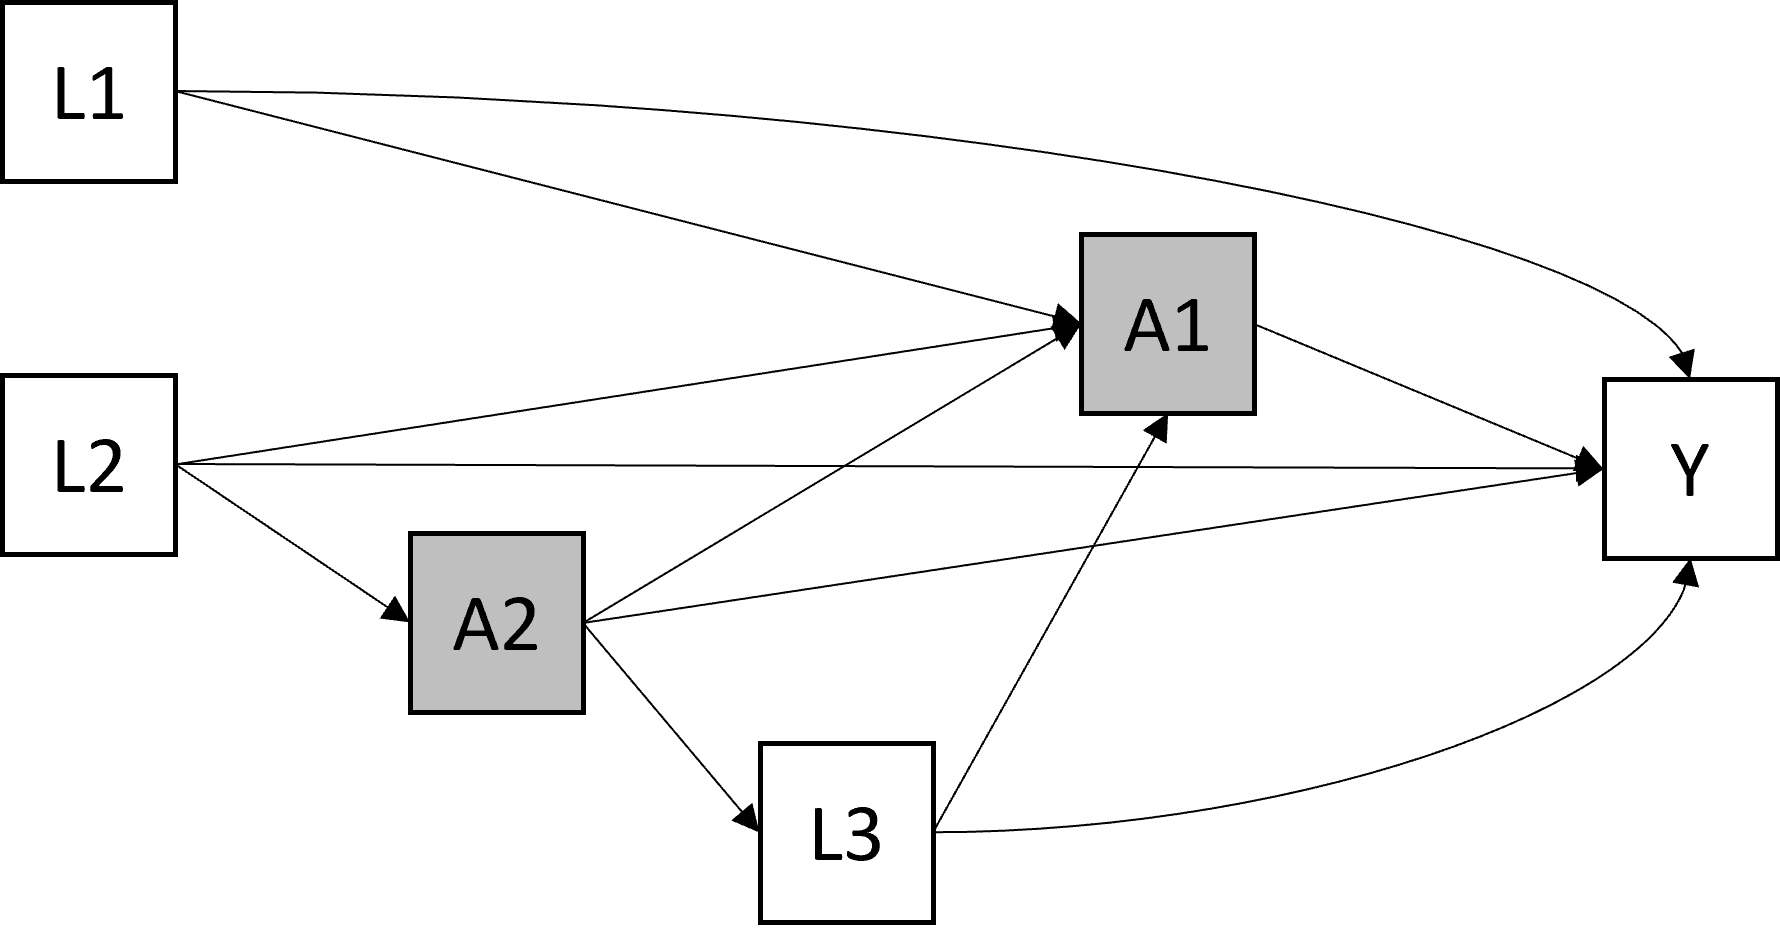
\includegraphics[width=0.5\textwidth,height=\textheight]{img/Image11.png}
\end{quote}

\hypertarget{interaction-avec-confusion-intermuxe9diaire}{%
\section{Interaction avec confusion intermédiaire}\label{interaction-avec-confusion-intermuxe9diaire}}

\hypertarget{interaction-et-muxe9diation}{%
\section{Interaction et médiation}\label{interaction-et-muxe9diation}}

\citet{vanderweele_three-way_2013}

\citet{vanderweele_unification_2014}

\hypertarget{ruxe9fuxe9rences}{%
\chapter{Références}\label{ruxe9fuxe9rences}}

  \bibliography{reference.bib}

\end{document}
